%%%%%%%%%%%%%%%%%%%%%%%%%%%%%%%%%%%%%%%%%%%%%%%%%%%%%%%%%%%%%%%%%%%%%%%%%%
%%
%% Toki Pona - lessons (English)
%% 
%%
%% apt-get install texlive-latex-base texlive-latex-extra texlive-luatex texlive-latex-extra texlive-pstricks rubber latex2html texlive-lang-german latex-xcolor
%% 
%%%%%%%%%%%%%%%%%%%%%%%%%%%%%%%%%%%%%%%%%%%%%%%%%%%%%%%%%%%%%%%%%%%%%%%%%%
\documentclass[a4paper, 10pt]{book} 
%\usepackage{ngerman}
\usepackage{ulem}
\usepackage{supertabular}
\usepackage[latin1]{inputenc}
% Indexverzeichnis erstellen:
\usepackage{makeidx}
\makeindex 
\usepackage{graphicx}
%%%%%%%%%%%%%%%%%%%%%%%%%%%%%%%%%%%%%%%%%%%%%%%%%%%%%%%%%%%%%%%%%%%%%%%%%%
% html is for the html tags 
\usepackage{html}
% hyperref is for the hyperlinks in PDF 
% and have to be the last packet
\usepackage{hyperref}
\usepackage{xcolor}
\hypersetup{%
	pdfauthor={ B. J. Knight, Robert Warnke},
	pdftitle={Toki Pona -- the language of good -- the simple way of life},
	pdfsubject={Toki Pona -- the language of good -- the simple way of life},
	pdfkeywords={Toki Pona, a akesi ala ale ali anpa ante anu awen e en ijo ike ilo insa jaki jan jelo jo kala kalama kama kasi ken kepeken kili kin kiwen ko kon kule kulupu kute la lape laso lawa  len lete li lili linja lipu loje lon luka lukin lupa ma mama mani meli mi mije moku moli monsi mu mun musi mute nanpa nasa nasin nena ni nimi noka o oko olin ona open pakala pali palisa pana pi pilin pimeja pini pipi poka poki pona sama seli selo seme sewi sijelo sike sin sina sinpin sitelen sona soweli suli suno supa suwi tan taso tawa telo tenpo toki tomo tu unpa uta utala walo wan waso wawa weka wile },
	colorlinks=true,
	urlcolor=blue,
	urlbordercolor=blue
}
%%%%%%%%%%%%%%%%%%%%%%%%%%%%%%%%%%%%%%%%%%%%%%%%%%%%%%%%%%%%%%%%%%%%%%%%%%
%%%%%%%%%%%%%%%%%%%%%%%%%%%%%%%%%%%%%%%%%%%%%%%%%%%%%%%%%%%%%%%%%%%%%%%%%%
%%%%%%%%%%%%%%%%%%%%%%%%%%%%%%%%%%%%%%%%%%%%%%%%%%%%%%%%%%%%%%%%%%%%%%%%%%
\makeindex
\begin{document}
%%%%%%%%%%%%%%%%%%%%%%%%%%%%%%%%%%%%%%%%%%%%%%%%%%%%%%%%%%%%%%%%%%%%%%%%%%
\setlength{\topmargin}{-19mm}
\setlength{\headheight}{5mm}
\setlength{\headsep}{10mm}
\setlength{\textheight}{245mm}
\setlength{\textwidth}{155mm}
\setlength{\oddsidemargin}{5mm}
\setlength{\evensidemargin}{-1mm}
\setlength{\footskip}{20mm}
\setlength{\parindent}{0mm}
\setlength{\parskip}{2.0ex plus 1.0ex minus 0.5ex}
\batchmode
%%%%%%%%%%%%%%%%%%%%%%%%%%%%%%%%%%%%%%%%%%%%%%%%%%%%%%%%%%%%%%%%%%%%%%%%%%
\title{
Toki Pona \\  \\ 
The Simplest Language in the World \\ 
Grammar and Vocabulary Lessons \\
}
\author{
Author of the original lessons: \\ B. J. Knight (jan Pije), USA \cite{www:Pije:01} \\  
\and
\LaTeX, Updates, Additions and \LaTeX layout: \\ Robert Warnke (jan Lope), Germany \cite{www:rowa:01} \\ 
\and
These lessons (first edition 2004) are based on the lessons of jan Pije (2003) and \\ 
the offical Toki Pona book (first English edition 2014) of Sonja Lang \cite{www:tokipona.org} 
}

%
\date
% \thanks{}
\today
\maketitle
\tableofcontents
%
%%%%%%%%%%%%%%%%%%%%%%%%%%%%%%%%%%%%%%%%%%%%%%%%%%%%%%%%%%%%%%%%%%%%%%%%%%
%%%%%%%%%%%%%%%%%%%%%%%%%%%%%%%%%%%%%%%%%%%%%%%%%%%%%%%%%%%%%%%%%%%%%%%%%%
\chapter{Lessons}
%%%%%%%%%%%%%%%%%%%%%%%%%%%%%%%%%%%%%%%%%%%%%%%%%%%%%%%%%%%%%%%%%%%%%%%%%%
%%%%%%%%%%%%%%%%%%%%%%%%%%%%%%%%%%%%%%%%%%%%%%%%%%%%%%%%%%%%%%%%%%%%%%%%%%
\section{Introduction}
%%%%%%%%%%%%%%%%%%%%%%%%%%%%%%%%%%%%%%%%%%%%%%%%%%%%%%%%%%%%%%%%%%%%%%%%%%
%
Sonja Lang created the language Toki Pona in the year 2001. 
Her aim was the minimalism. 
Toki Pona consists of only about 120 words, which are not altered. 
In accordance with the position in the sentence, the words can vary their significance. 
To describe more details you have to combine the words.

It is not the goal of Toki Pona to describe complex issues. 
Dissertations and scientific papers will never written in Toki Pona. 
Lawyers, bureaucrats, theologians and politicians are be warned of the side-effect of this language.

It is not he aim of Toki Pona to solve the communication problems in the world. 
But you can learn this language in a month. 
Toki Pona is easy in an intelligent way and yoga for the brain. 
People who hate nested subordinate clauses and commas will certainly have fun with Toki Pona.

Toki Pona has evolved since 2001. 
There are also slangs, which hinder the understanding. 
Therefore these lessons are based on the official Toki Pona book \cite{www:tokipona.org} by Sonja Lang (2014) and the updated tutorials from BJ Knight (jan Pije) \cite{www:Pije:01}.

So have fun with the lessons and learning of Toki Pona. 
For learning vocabulary helps Memrise \cite{www:memrise:01}. Related Links Toki Pona can be found on the website \cite{www:rowa:01}. 
A dictionary can be found here \cite{www:rowa:01}. 

You can use the tool \textit{Toki Pona Parser} (\cite{www:rowa:02}) for spelling, grammar check and ambiguity check of Toki Pona sentences 

Maybe only one natural language can be compared to Toki Pona. 
It is the language of the Pirahá (\cite{www:piraha:01}). 
For example this language has no recursion. 

\textit{toki pona li pona, tawa sina.}
%
%%%%%%%%%%%%%%%%%%%%%%%%%%%%%%%%%%%%%%%%%%%%%%%%%%%%%%%%%%%%%%%%%%%%%%%%%%
% eof

%%%%%%%%%%%%%%%%%%%%%%%%%%%%%%%%%%%%%%%%%%%%%%%%%%%%%%%%%%%%%%%%%%%%%%%%%%
\label{'pronunciation_alphabet'}
\section{Alphabet, Punctuation Marks}
%%%%%%%%%%%%%%%%%%%%%%%%%%%%%%%%%%%%%%%%%%%%%%%%%%%%%%%%%%%%%%%%%%%%%%%%%%
%
% There are \textbf{fourteen letters} in the Toki Pona alphabet.
%%%%%%%%%%%%%%%%%%%%%%%%%%%%%%%%%%%%%%%%%%%%%%%%%%%%%%%%%%%%%%%%%%%%%%%%%%
\subsection*{Consonants}
\index{consonant}
%%%%%%%%%%%%%%%%%%%%%%%%%%%%%%%%%%%%%%%%%%%%%%%%%%%%%%%%%%%%%%%%%%%%%%%%%%
%
Except for \textit{j}, all the consonants are pronounced like in English. 
\textit{j} is always pronounced just like the letter \textit{y}. 

\begin{supertabular}{p{2cm}|ll}
\textbf{letter}   &&    \textbf{pronounced as in} \\ % no-dictionary
k && \textbf{k}ill  \\ % no-dictionary
l && \textbf{l}et   \\ % no-dictionary
m && \textbf{m}et   \\ % no-dictionary
n && \textbf{n}et   \\ % no-dictionary
p && \textbf{p}it   \\ % no-dictionary
s && \textbf{s}ink  \\ % no-dictionary
t && \textbf{t}oo   \\ % no-dictionary
w && \textbf{w}et   \\ % no-dictionary
j && \textbf{y}et   \\ % no-dictionary
\end{supertabular} 

%%%%%%%%%%%%%%%%%%%%%%%%%%%%%%%%%%%%%%%%%%%%%%%%%%%%%%%%%%%%%%%%%%%%%%%%%%
\subsection*{Vowels}
\index{vowel}
%%%%%%%%%%%%%%%%%%%%%%%%%%%%%%%%%%%%%%%%%%%%%%%%%%%%%%%%%%%%%%%%%%%%%%%%%%
%
Toki Pona's vowels are quite unlike English's. 

Toki Pona's vowels are quite unlike English's. Whereas vowels in English are quite arbitrary and can be pronounced many different ways depending on the word, Toki Pona's vowels are all regular and never change pronunciation. 
If you're familiar with Italian, Spanish, Esperanto, or certain other languages, then your work is already done. The vowels are the same in Toki Pona as they are in these languages. 

\begin{supertabular}{p{2cm}|ll}
\textbf{letter}   &&    \textbf{pronounced as in} \\ % no-dictionary
a   &&    f\textbf{a}ther \\ % no-dictionary
e   &&    m\textbf{e}t    \\ % no-dictionary
i   &&    p\textbf{ee}l   \\ % no-dictionary
o   &&    m\textbf{o}re   \\ % no-dictionary
u   &&    f\textbf{oo}d   \\ % no-dictionary
\end{supertabular} 

%
%%%%%%%%%%%%%%%%%%%%%%%%%%%%%%%%%%%%%%%%%%%%%%%%%%%%%%%%%%%%%%%%%%%%%%%%%%
\subsection*{The More Advanced Stuff}
\index{lowercase letter}
\index{letter!lowercase}
\index{capital letter}
\index{letter!capital}
%%%%%%%%%%%%%%%%%%%%%%%%%%%%%%%%%%%%%%%%%%%%%%%%%%%%%%%%%%%%%%%%%%%%%%%%%%
%
All official Toki Pona words are never capitalized. 
They are lowercase even at the beginning of the sentence! 
The only time that capital letters are used is when you are using unofficial words, like the names of people or places or religions. 
%
%
%%%%%%%%%%%%%%%%%%%%%%%%%%%%%%%%%%%%%%%%%%%%%%%%%%%%%%%%%%%%%%%%%%%%%%%%%%
\subsection*{Special Characters}
\index{special character}
\index{character!special}
%%%%%%%%%%%%%%%%%%%%%%%%%%%%%%%%%%%%%%%%%%%%%%%%%%%%%%%%%%%%%%%%%%%%%%%%%%
%

\begin{supertabular}{p{2cm}|ll} 
\textbf{.} && \textit{separator}: A declarative sentence ends with a full stop. \\ % no-dictionary
\textbf{!} && \textit{separator}: An imperative or an interjection sentence ends with \\ &&  an exclamation mark. \\ % no-dictionary
\textbf{?} && \textit{separator}: An questions always ends in a question mark. \\ % no-dictionary
\textbf{:} && \textit{separator}: A colon is between an hint sentences and a sentences. \\  % no-dictionary
\textbf{,} && \textit{separator}: A comma is used after an 'o' to address people. \\ && Optionally, it can be inserted before a preposition. \\ % no-dictionary
\end{supertabular} \\

%
%%%%%%%%%%%%%%%%%%%%%%%%%%%%%%%%%%%%%%%%%%%%%%%%%%%%%%%%%%%%%%%%%%%%%%%%%%
\subsection*{Separators}
\index{separator}
%%%%%%%%%%%%%%%%%%%%%%%%%%%%%%%%%%%%%%%%%%%%%%%%%%%%%%%%%%%%%%%%%%%%%%%%%%
%
In these lessons, special characters are referred to as separators. 
Separators separate phrases from each other. 
For example, a dot separates a sentence from the next sentence. 
In Toki Pona also special words serve as separators. 
In other lessons these words are also called 'particles'.

%
%%%%%%%%%%%%%%%%%%%%%%%%%%%%%%%%%%%%%%%%%%%%%%%%%%%%%%%%%%%%%%%%%%%%%%%%%%
\subsection*{Types of Sentences}
%
\index{sentence!type}
\index{declarative sentence}
\index{interrogative sentence}
\index{question sentence}
\index{imperative sentence}
\index{exclamatory sentence}
\index{interjection sentence}
\index{headlines}
\index{title}
\index{punctuation mark}
%%%%%%%%%%%%%%%%%%%%%%%%%%%%%%%%%%%%%%%%%%%%%%%%%%%%%%%%%%%%%%%%%%%%%%%%%%
%
Toki Pona has how many languages, different types of sentences. 

Most sentences are declarative sentences and end with a period. 
Declarative sentences make statements or an assumptions. 

Question sentences are interrogative sentences that formulate a question. 
They end with a question mark. 

Imperative sentences are sentences that formulate a command. 
They end with an exclamation mark.

Exclamatory sentences (interjections) are sentences that express admiration or astonishment. 
This also includes greetings. 
They end with an exclamation mark or a period.

Headlines (titles) are usually not complete sentences and do not end with a punctuation mark.

Please always pay attention to correct punctuation marks. Wrong or missing
Punctuation marks impair the intelligibility.

%
\newpage
%%%%%%%%%%%%%%%%%%%%%%%%%%%%%%%%%%%%%%%%%%%%%%%%%%%%%%%%%%%%%%%%%%%%%%%%%%
\subsection*{Practice (Answers: Page~\pageref{'pronunciation_alphabet'})}
%%%%%%%%%%%%%%%%%%%%%%%%%%%%%%%%%%%%%%%%%%%%%%%%%%%%%%%%%%%%%%%%%%%%%%%%%%

Please write down your answers and check them afterwards. 

\begin{supertabular}{p{5cm}|ll}
What are separators? &&                                      \\ % no-dictionary
 && \\ % no-dictionary
Which phrase has no punctuation character at the end? &&     \\ % no-dictionary
 && \\ % no-dictionary
Which separator is at the end of a declarative sentence? &&  \\ % no-dictionary
 && \\ % no-dictionary
When are official \textit{toki pona} words capitalized? &&   \\ % no-dictionary
 && \\ % no-dictionary
What is usually not allowed before or after a separator? &&  \\ % no-dictionary

\end{supertabular} \\% no-dictionary
%
%%%%%%%%%%%%%%%%%%%%%%%%%%%%%%%%%%%%%%%%%%%%%%%%%%%%%%%%%%%%%%%%%%%%%%%%%%
% eof

%%%%%%%%%%%%%%%%%%%%%%%%%%%%%%%%%%%%%%%%%%%%%%%%%%%%%%%%%%%%%%%%%%%%%%%%%%
\section{Basic Sentences}
%%%%%%%%%%%%%%%%%%%%%%%%%%%%%%%%%%%%%%%%%%%%%%%%%%%%%%%%%%%%%%%%%%%%%%%%%%
\subsection*{Vocabulary}
%%%%%%%%%%%%%%%%%%%%%%%%%%%%%%%%%%%%%%%%%%%%%%%%%%%%%%%%%%%%%%%%%%%%%%%%%%
\index{\textit{jan}}
\index{\textit{mi}}
\index{\textit{moku}}
\index{\textit{sina}}
\index{\textit{suno}}
\index{\textit{telo}}
\index{\textit{pona}}
\index{\textit{suli}}
\index{\textit{li}}
\index{I}
\index{me}
\index{food}
\index{eat}
\index{drink}
\index{you}
\index{sun}
\index{light}
\index{water}
\index{liquid}
\index{good}
\index{simple}
\index{fix}
\index{repair}
\index{big}
\index{tall}
\index{long}
\index{important}
\begin{supertabular}{p{2,5cm}|ll}
\textbf{\dots jan} && \textit{adjective}: human, somebody's, personal, of people \\ % no-dictionary
\textbf{\dots jan} && \textit{adverb}: human, somebody's, personal, of people \\ % no-dictionary
\textbf{jan} && \textit{noun}: person, people, human, being, somebody, anybody \\ % no-dictionary
\textbf{jan (e \dots)} && \textit{verb transitive}: to personify, to humanize, to personalize \\ % no-dictionary
 && \\ % no-dictionary
\textbf{\dots li \dots} && \textit{separator}: A 'li' is between any subject except 'mi' and 'sina' and its verb. \\ && Don't use 'li' before or after an other separator. \\ % no-dictionary
 && \\ % no-dictionary
\textbf{mi} && \textit{personal pronoun}: I, we  \\ 
\textbf{\dots mi} && \textit{possessive pronoun}: my, our \\  
\textbf{\dots e mi} && \textit{reflexive pronoun}: myself, ourselves  \\ 
 && \\ % no-dictionary
\textbf{\dots moku} && \textit{adjective}: eating \\ % no-dictionary
\textbf{\dots moku} && \textit{adverb}: eating \\ % no-dictionary
\textbf{moku} && \textit{noun}: food, meal \\ % no-dictionary
\textbf{moku (e \dots)} && \textit{verb transitive}: to eat, to drink, to swallow, to ingest, to consume \\ % no-dictionary
 && \\ % no-dictionary
\textbf{ona} && \textit{personal pronoun}: she, he, it, they \\ % no-dictionary
\textbf{\dots ona} && \textit{possessive pronoun}: her, his, its \\  % no-dictionary
\textbf{\dots e ona} && \textit{reflexive pronoun}: himself, herself, itself, themselves \\  
 && \\ % no-dictionary 
\textbf{\dots pona} && \textit{adjective}: good, simple, positive, nice, correct, right \\ % no-dictionary
\textbf{\dots pona} && \textit{adverb}: good, simple, positive, nice, correct, right \\ % no-dictionary
\textbf{pona} && \textit{noun}: good, simplicity, positivity \\ % no-dictionary
\textbf{pona (e \dots)} && \textit{verb transitive}: to improve, to fix, to repair, to make good \\ % no-dictionary
 && \\ % no-dictionary
\textbf{sina} && \textit{personal pronoun}: you \\ % no-dictionary
\textbf{\dots sina} && \textit{possessive pronoun}: yours \\  % no-dictionary
\textbf{\dots e sina} && \textit{reflexive pronoun}: yourself, yourselves \\  
 && \\ % no-dictionary
\textbf{\dots suno} && \textit{adjective}: sunny, sunnily \\ % no-dictionary
\textbf{\dots suno} && \textit{adverb}: sunny, sunnily \\ % no-dictionary
\textbf{suno} && \textit{noun}: sun, light \\ % no-dictionary
\textbf{suno (e \dots)} && \textit{verb transitive}: to light, to illumine \\ % no-dictionary
 && \\ % no-dictionary
\textbf{\dots suli} && \textit{adjective}: big, tall, long, adult, important \\ % no-dictionary
\textbf{\dots suli} && \textit{adverb}: big, tall, long, adult, important \\ % no-dictionary
\textbf{suli} && \textit{noun}: size \\ % no-dictionary
\textbf{suli (e \dots)} && \textit{verb transitive}: to enlarge, to lengthen \\ % no-dictionary
 && \\ % no-dictionary
\textbf{\dots telo} && \textit{adjective}: wett, slobbery, moist, damp, humid, sticky, sweaty, dewy, drizzly \\ % no-dictionary
\textbf{\dots telo} && \textit{adverb}: wett, slobbery, moist, damp, humid, sticky, sweaty, dewy, drizzly \\ % no-dictionary
\textbf{telo} && \textit{noun}: water, liquid, juice, sauce \\ % no-dictionary
\textbf{telo (e \dots)} && \textit{verb transitive}: to water, to wash with water, to put water to, to melt, to liquify \\ % no-dictionary
 && \\ % no-dictionary
\textbf{'} && \textit{unofficial}: For clarification the missing verb 'to be' can be marked with an apostrophe.  \\ % no-dictionary
\end{supertabular} \\
%
\newpage
%%%%%%%%%%%%%%%%%%%%%%%%%%%%%%%%%%%%%%%%%%%%%%%%%%%%%%%%%%%%%%%%%%%%%%%%%%
\index{singular}
\index{plural}
\index{Tense}
\index{noun}
\index{pronoun}
\index{personal pronoun}
\index{possessive pronoun}
\index{reflexive pronoun}
\index{adjective}
\index{verb}
\subsection*{The Ambiguity of Toki Pona}
%%%%%%%%%%%%%%%%%%%%%%%%%%%%%%%%%%%%%%%%%%%%%%%%%%%%%%%%%%%%%%%%%%%%%%%%%%
%
Do you see how several of the words in the vocabulary have multiple meanings? 
For example, \textit{suli} can mean either 'long', 'tall', 'big', 'important' or 'the size'. 
By now, you might be wondering, 'What's going on? How can one word mean so many different things?' 

Welcome to the world of Toki Pona! The truth is that lots of words are like this in Toki Pona. 
Because the language has such a small vocabulary and is so basic, the ambiguity is inevitable. 
However, this vagueness is not necessarily a bad thing. Because of the vagueness, a speaker of Toki Pona is forced to focus on the very basic, unaltered aspect of things, rather than focusing on many minute details. 

Another way that Toki Pona is ambiguous is that it can not specify whether a word is singular or plural. 
For example, \textit{jan} can mean either 'person' or 'people'. 
If you've decided that Toki Pona is too arbitrary and that not having plurals is simply the final straw, don't be so hasty. 
Toki Pona is not the only language that doesn't specify whether a noun is plural or not. 
Japanese, for example, does the same thing. 

Toki Pona has no Tenses. 
The verbs don't change. 
If it's absolutely necessary, there are ways of saying that something happened in the past, present, or future. 

As you can see in the vocabulary list, most words can be used in different word types. 
They remain unchanged. 
The word part is derived from the position in the sentence. 
In this lesson, we will deal with nouns, pronouns, verbs, adjectives and a special separator. 

A noun is a word for a person, place or thing. 
An adjective is a word that describes a noun. 
A verb describes an action. 

Pronouns are proxies for different types of words. 
They are used in the same place as the word to be represented and have the same grammatical characteristics as this one.
Pronouns are not words of content, but they denote persons or things by referring to the context. 
Personal pronouns (I, you, \dots) represent nouns. 
Possessive pronouns (my, your, \dots) represent adjectives. 
In the next few lessons we will learn more about other types of pronouns. 

% 
%%%%%%%%%%%%%%%%%%%%%%%%%%%%%%%%%%%%%%%%%%%%%%%%%%%%%%%%%%%%%%%%%%%%%%%%%%
\index{\textit{mi}}
\index{\textit{sina}}
\index{\textit{mi}!subject}
\index{\textit{sina}!subject}
\index{subject}
\index{subject phrase}
\index{subject!\textit{mi}}
\index{subject!\textit{sina}}
\index{predicate}
\index{predicate phrase}
\index{verb!to be}
\index{be}
\label{'predicate'}
\subsection*{The Personal Pronouns \textit{mi} or \textit{sina} as Subject}
%%%%%%%%%%%%%%%%%%%%%%%%%%%%%%%%%%%%%%%%%%%%%%%%%%%%%%%%%%%%%%%%%%%%%%%%%%
%
With the pronoun \textit{mi} or the pronoun \textit{sina} at the beginning and a subsequent verb a simple sentence in toki pona is already complete. 
A declarative sentence ends with a full stop. 
Toki Pona has no nested subordinate clauses and nearly no commas. 

\begin{supertabular}{p{5,5cm}|ll}
mi moku. && I eat. \\
sina pona. && You fix. \\
\end{supertabular} 

In these sentences pronouns \textit{mi} and \textit{sina} are in each case the subject phrase. 
In Toki Pona, a subject phrase is always at the beginning of the sentence. 
In these examples, the subject phrases consist of only one subject (\textit{mi} or \textit{sina}).

The subject is the carrier of the action, process or state. 
It is the most important addition to the verb in the sentence, a complete sentence always contains a subject. 
You ask for the subject with whom or what.

The verbs \textit{moku} and \textit{pona} form the predicate phrase in these examples.  
The predicate is a core element in a sentence and is the statement of the sentence.
In most languages, a predicate is formed by a verb, but this is not mandatory in all languages. 
As we will soon see, in Toki Pona the predicate is not necessarily formed by a verb. 
The difference between verb and predicate is that verb designates a word part and predicate designates a grammatical function.
A predicate and possible objects form a predicate phrase. 
%
%%%%%%%%%%%%%%%%%%%%%%%%%%%%%%%%%%%%%%%%%%%%%%%%%%%%%%%%%%%%%%%%%%%%%%%%%%
\index{apostrophe}
\subsubsection*{The Lack of the verb 'to be'}
%%%%%%%%%%%%%%%%%%%%%%%%%%%%%%%%%%%%%%%%%%%%%%%%%%%%%%%%%%%%%%%%%%%%%%%%%%
%
One of the first principles you'll need to learn about Toki Pona is that there is no form of the verb 'to be' like there is in English. 
By the missing 'to be' the verb slot can be empty and after \textit{mi} or \textit{sina} can follow also a noun or adjective. 
In these lessons, the term' slot' is used to indicate a valid position of a word type in the sentence.

Regular sentences can also be formed in other languages without a verb appearing in them. 
Examples are Russian and Arabic. 
A noun then functions as a predicate noun or an adjective serves as predicate adjective.
But this noun or adjective does not become a verb. 
An empty verb slot cannot, however, form a predicate phrase on its own. 
A noun or adjective must follow. 
That is, directly after \textit{mi} or \textit{sina} the sentence cannot be finished yet.

The missing verb 'to be' or the empty verb-slot is marked with an apostrophe in these lessons. 

\begin{supertabular}{p{5cm}|ll}
mi moku. && I eat.  \\
mi ' moku. && I am food. \\  
sina pona. && You fix. \\
sina ' pona. && You are good. \\  
\end{supertabular} 

Because Toki Pona lacks 'to be', the exact meaning is lost. 
\textit{moku} in this sentence could be a verb, or it could be a noun; just as \textit{pona} could be an adjective or could be a verb. 
In situations such as these, the listener must rely on context. 
After all, how often do you hear someone say 'I am food.'? 
I hope not very often! You can be fairly certain that \textit{mi moku} means 'I'm eating'. 
%
%%%%%%%%%%%%%%%%%%%%%%%%%%%%%%%%%%%%%%%%%%%%%%%%%%%%%%%%%%%%%%%%%%%%%%%%%%
\index{\textit{li}}
\index{subject!\textit{mi}}
\index{subject!\textit{sina}}
\index{\textit{mi}!subject}
\index{\textit{sina}!subject}
\subsection*{The Separator \textit{li} }
%%%%%%%%%%%%%%%%%%%%%%%%%%%%%%%%%%%%%%%%%%%%%%%%%%%%%%%%%%%%%%%%%%%%%%%%%%
%
For sentences that don't use the personal pronouns \textit{mi} or \textit{sina} as the subject, there is one small catch that you'll have to learn. 
Look at how \textit{li} is used. 
\textit{li} is a grammatical word that separates the subject phrase from the predicate phrase. 
Th predicate marker \textit{li} is only used when the subject is not \textit{mi} or \textit{sina}. 
Although the separator \textit{li} might seem worthless right now, as you continue to learn Toki Pona you will see that some sentences could be very confusing if \textit{li} weren't there. 

\begin{supertabular}{p{5cm}|ll}
telo li pona. && Water is cleaning. \\
suno li suno. && The sun is shining. \\
moku li ' pona. && The food is good. \\ 
ona li ' moku. && It is food. \\
\end{supertabular} 

Because of the lacks of 'to be', after \textit{li} can not only be a verb, it can follow a noun or adjective as well. 
As already written, an empty verb slot cannot form a predicate phrase on its own. 
A noun or adjective must follow. 
That is, directly after \textit{li} the sentence can not yet be finished or an object can follow.
%
\newpage
%%%%%%%%%%%%%%%%%%%%%%%%%%%%%%%%%%%%%%%%%%%%%%%%%%%%%%%%%%%%%%%%%%%%%%%%%%
\subsection*{Practice 3 (Answers: Page~\pageref{'basic_sentences'})}
%%%%%%%%%%%%%%%%%%%%%%%%%%%%%%%%%%%%%%%%%%%%%%%%%%%%%%%%%%%%%%%%%%%%%%%%%%
%

Please write down your answers and check them afterwards. 

\begin{supertabular}{p{5cm}|ll}
What is a verb &&  \\ % no-dictionary
What is a noun? &&   \\ % no-dictionary
What is \textit{li} used for?  &&   \\ % no-dictionary
What does a personal pronoun replace? &&  \\ % no-dictionary
How to recognize nouns, pronouns, verbs and adjectives in \textit{toki pona}? &&  \\ % no-dictionary
What is a subject?  &&   \\ % no-dictionary
After which subject phrases is \textit{li} not used?  &&  \\ % no-dictionary
Where does the subject stand in the sentence?  &&    \\ % no-dictionary
Can an empty verb slot alone form a predicate? &&    \\ % no-dictionary
When can a verb slot be empty?  &&     \\ % no-dictionary
What is a predicate?  &&     \\ % no-dictionary
A complete sentence in \textit{toki pona} always contains\dots  &&     \\ % no-dictionary
What kinds of words can be used in \textit{toki pona} to form a predicate? &&   \\ % no-dictionary
What is an adjective?  &&    \\ % no-dictionary
Where are possible adjective slots?  &&    \\  % no-dictionary
Why can't a sentence be ended after \textit{li}? &&  \\ % no-dictionary
\end{supertabular} 

Try to translate these sentences. 
You can use the tool \textit{Toki Pona Parser} (\cite{www:rowa:02}) for spelling and grammar check. 

\begin{supertabular}{p{5cm}|ll}
People are good. && \\ % no-dictionary
I'm eating. &&  \\ % no-dictionary
You're tall. &&  \\ % no-dictionary
Water is simple. &&  \\ % no-dictionary
The lake is big. &&\\ % no-dictionary
 && \\ % no-dictionary
suno li ' suli. &&  \\% no-dictionary
mi ' suli. &&  \\% no-dictionary
jan li moku. &&  \\% no-dictionary
\end{supertabular} \\% no-dictionary
%
%%%%%%%%%%%%%%%%%%%%%%%%%%%%%%%%%%%%%%%%%%%%%%%%%%%%%%%%%%%%%%%%%%%%%%%%%%
% eof

%%%%%%%%%%%%%%%%%%%%%%%%%%%%%%%%%%%%%%%%%%%%%%%%%%%%%%%%%%%%%%%%%%%%%%%%%%
\section{Direct Objects}
%
%%%%%%%%%%%%%%%%%%%%%%%%%%%%%%%%%%%%%%%%%%%%%%%%%%%%%%%%%%%%%%%%%%%%%%%%%%
\subsection*{Vocabulary}
%%%%%%%%%%%%%%%%%%%%%%%%%%%%%%%%%%%%%%%%%%%%%%%%%%%%%%%%%%%%%%%%%%%%%%%%%%
%
\begin{supertabular}{p{2,5cm}|ll}
%
\index{e}
\textbf{\dots e \dots} && \textit{separator}: An 'e' introduces a direct object. \\ && Don't use 'e' before or after the other separators. \\ % no-dictionary
 && \\ % no-dictionary
%
\index{ijo}
\textbf{\dots ijo} && \textit{adjective}: of something \\ % no-dictionary
\textbf{\dots ijo} && \textit{adverb}: of something \\ % no-dictionary
\textbf{ijo} && \textit{noun}: thing, something, stuff, anything, object \\ % no-dictionary
\textbf{ijo (e \dots)} && \textit{verb transitive}: to objectify \\ % no-dictionary
 && \\ % no-dictionary
%
\index{ilo}
\textbf{\dots ilo} && \textit{adjective}: useful \\ % no-dictionary
\textbf{\dots ilo} && \textit{adverb}: usefully \\ % no-dictionary
\textbf{ilo} && \textit{noun}: tool, device, machine, thing used for a specific purpose \\ % no-dictionary
 && \\ % no-dictionary
%
\index{jo}
\textbf{\dots jo} && \textit{adjective}: private, personal \\ % no-dictionary
\textbf{jo} && \textit{noun}: having, possessions, content \\ % no-dictionary
\textbf{jo (e \dots)} && \textit{verb transitive}: to have, to contain \\ % no-dictionary
 && \\ % no-dictionary
%
\index{kili}
\textbf{\dots kili} && \textit{adjective}: fruity \\ % no-dictionary
\textbf{\dots kili} && \textit{adverb}: fruity \\ % no-dictionary
\textbf{kili} && \textit{noun}: fruit, pulpy vegetable, mushroom \\ % no-dictionary
 && \\ % no-dictionary
%
\index{lukin}
\textbf{\dots lukin} && \textit{adjective}: visual(ly) \\ % no-dictionary
\textbf{\dots lukin} && \textit{adverb}: visual(ly) \\ % no-dictionary
\textbf{lukin} && \textit{noun}: view, look, glance, sight, gaze, glimpse, seeing, vision \\ % no-dictionary
\textbf{lukin} && \textit{verb intransitive}: to look, to watch out, to pay attention \\ % no-dictionary
\textbf{lukin (e \dots)} && \textit{verb transitive}: to see, to look at, to watch, to read \\ % no-dictionary
\textbf{lukin \dots} && \textit{auxiliary verb}: to seek to, try to, look for \\ % no-dictionary
 && \\ % no-dictionary
%
\index{ma}
\textbf{\dots ma} && \textit{adjective}: countrified, outdoor, alfresco, open-air \\ % no-dictionary
\textbf{ma} && \textit{noun}: land, earth, country, (outdoor) area \\ % no-dictionary
 && \\ % no-dictionary
%
\index{pakala}
\textbf{\dots pakala} && \textit{adjective}: destroyed, ruined, demolished, shattered, wrecked \\ % no-dictionary
\textbf{\dots pakala} && \textit{adverb}: destroyed, ruined, demolished, shattered, wrecked \\ % no-dictionary
\textbf{pakala} && \textit{noun}: blunder, accident, mistake, destruction, damage, breaking \\ % no-dictionary
\textbf{pakala} && \textit{verb intransitive}: to screw up, to fall apart, to break \\ % no-dictionary
\textbf{pakala (e \dots)} && \textit{verb transitive}: to screw up, to ruin, to break, to hurt, to injure, to damage \\ % no-dictionary
 && \\ % no-dictionary
%
\index{unpa}
\textbf{\dots unpa} && \textit{adjective}: erotic, sexual \\ % no-dictionary
\textbf{\dots unpa} && \textit{adverb}: erotic, sexual \\ % no-dictionary
\textbf{unpa} && \textit{noun}: sex, sexuality \\ % no-dictionary
\textbf{unpa} && \textit{verb intransitive}: to have sex \\ % no-dictionary
\textbf{unpa (e \dots)} && \textit{verb transitive}: to have sex with, to sleep with, to fuck \\ % no-dictionary
 && \\ % no-dictionary
%
\index{wile}
%\textbf{\dots wile} && \textit{adjective}: necessary \\ % no-dictionary
%\textbf{\dots wile} && \textit{adverb}: necessary \\ % no-dictionary
\textbf{wile} && \textit{noun}: desire, need, will \\ % no-dictionary
\textbf{wile (e \dots)} && \textit{verb transitive}: to want, need, wish, have to, must, will, should \\ % no-dictionary
\textbf{wile \dots} && \textit{auxiliary verb}: to want, need, wish, have to, must, will, should \\ % no-dictionary
\end{supertabular} \\
%
\newpage
%%%%%%%%%%%%%%%%%%%%%%%%%%%%%%%%%%%%%%%%%%%%%%%%%%%%%%%%%%%%%%%%%%%%%%%%%%
\subsection*{Transitive Verbs, the Separator \textit{e} and Direct Objects}
%
\index{object!direct}
\index{verb!transitive}
\index{transitive verb}
\index{\textit{e}}
%%%%%%%%%%%%%%%%%%%%%%%%%%%%%%%%%%%%%%%%%%%%%%%%%%%%%%%%%%%%%%%%%%%%%%%%%%
%
We saw how phrases such as \textit{mi moku} could have two potential meanings. 
'I'm eating' or 'I am food'. 
There is one way to specify that you want to say. 

\begin{supertabular}{p{5,5cm}|ll}
mi moku e kili. && I eat fruit. \\
\end{supertabular} 

Also we discussed how \textit{sina pona}, like \textit{mi moku}, has two possible meanings. 
'You are good' or 'You're fixing'. 
Normally, it would mean 'You are good' simply because no one really says 'I'm fixing' without actually telling what it is that they are trying to fix. 

\begin{supertabular}{p{5,5cm}|ll}
ona li pona e ilo. && She's fixing the machine. \\
mi pona e ijo. && I'm fixing something. \\
\end{supertabular} 

Only a (composite) verb can stand in front of the \textit{e}. 
More specifically, it is a slot for a transitive verb. 
Transitive verbs are verbs after which a direct object (accusative object) can stand. 
A transitive verb does something to the direct object. 

The separator \textit{e} preface the direct object.
An object is an optional record supplement. 
A direct object is most strongly influenced by the action (i. e. the predicate).
Your can ask for direct object (accusative object) by' Who' or' What' (' What does she repair?'').
The direct object is part of the predicate phrase. 

In the direct object is the first slot after the separator \textit{e} always a noun or pronoun slot.
In the above examples the noun slots were filled with \textit{kili} and \textit{ijo}. 

%
%%%%%%%%%%%%%%%%%%%%%%%%%%%%%%%%%%%%%%%%%%%%%%%%%%%%%%%%%%%%%%%%%%%%%%%%%%
\subsection*{Reflexive Pronouns}
%
\index{reflexive pronoun}
\index{pronoun!reflexive}
\index{pronoun!personal}
\index{\textit{mi}!reflexive pronoun}
\index{\textit{sina}!reflexive pronoun}
\index{\textit{ona}!reflexive pronoun}
%%%%%%%%%%%%%%%%%%%%%%%%%%%%%%%%%%%%%%%%%%%%%%%%%%%%%%%%%%%%%%%%%%%%%%%%%%

A reflexive pronoun represents the subject in the direct object. 
So a slot for a reflective pronoun is located after the separator \textit{e}. 
In the following example, \textit{ona} is a reflexive pronoun, since it refers to the subject \textit{jan}. 

\begin{supertabular}{p{5,5cm}|ll}
jan li telo e ona. && A person washes himself. \\
\end{supertabular}

In this sentence the first \textit{mi} is a personal pronoun.
The \textit{mi} after the \textit{e} is a reflexive pronoun. 

\begin{supertabular}{p{5,5cm}|ll}
mi telo e mi. && I wash myself. \\
\end{supertabular}

Here a sentence with \textit{sina} as personal and reflective pronouns

\begin{supertabular}{p{5,5cm}|ll}
sina telo e sina. && You wash yourself. \\
\end{supertabular}

Here a sentence with \textit{ona} as personal and reflective pronouns

\begin{supertabular}{p{5,5cm}|ll}
ona telo e ona. && She washes herself. \\
\end{supertabular}

%%%%%%%%%%%%%%%%%%%%%%%%%%%%%%%%%%%%%%%%%%%%%%%%%%%%%%%%%%%%%%%%%%%%%%%%%%
% \newpage
\index{sentence!compound}
\subsection*{Compound Sentences}
%%%%%%%%%%%%%%%%%%%%%%%%%%%%%%%%%%%%%%%%%%%%%%%%%%%%%%%%%%%%%%%%%%%%%%%%%%
%
There are two ways to make compound sentences in Toki Pona; one way involves using \textit{li}, and the other way involves using \textit{e}. 
Since you've now studied both of these words, we'll cover how to use both of them to make compound sentences. 

%%%%%%%%%%%%%%%%%%%%%%%%%%%%%%%%%%%%%%%%%%%%%%%%%%%%%%%%%%%%%%%%%%%%%%%%%%
\index{predicate phrases¡several}
%
\label{'multiple_li'}
\subsubsection*{Several \textit{li} Separators for Several Predicate Phrases}
%%%%%%%%%%%%%%%%%%%%%%%%%%%%%%%%%%%%%%%%%%%%%%%%%%%%%%%%%%%%%%%%%%%%%%%%%%
%

It is possible to use the separator \textit{li} several times in a sentence. 
Each separator \textit{li} starts a new predicate phrase. 
This allows you to assign several actions or properties to one subject. 

\begin{supertabular}{p{5,5cm}|ll}
ona li ' pona li unpa. && He's awesome and has sex. \\
\end{supertabular} 

In the next example the separator \textit{li} is still omitted before \textit{moku} because the subject of the sentence is the personal pronoun \textit{mi}, we still use it before the second predicate, \textit{pakala}. 
Without the separator \textit{li} there, the sentence would be chaotic and confusing. 
Compound sentences with personal pronoun \textit{sina} as subject follow this same pattern. 

\begin{supertabular}{p{5,5cm}|ll}
mi moku li pakala. && I eat and destroy. \\
\end{supertabular} 

Predicate phrases are not nested. You can change the order. \\
ona li moku li ' pona. = ona li ' pona li moku. 

Each predicate phrase can of course contain direct objects. 

\begin{supertabular}{p{5,5cm}|ll}
mi moku e moku li lukin e ma. && I eat the food and look at the landscape. \\
\end{supertabular} 

The official Toki Pona book recommends to use only one predicate phrase for the personal pronouns \textit{mi} or \textit{sina} as subject. 
%
%%%%%%%%%%%%%%%%%%%%%%%%%%%%%%%%%%%%%%%%%%%%%%%%%%%%%%%%%%%%%%%%%%%%%%%%%%
\index{object!several}
\label{'multiple_e'}
\subsubsection*{Several \textit{e} Separators for Several direct Objects}
%%%%%%%%%%%%%%%%%%%%%%%%%%%%%%%%%%%%%%%%%%%%%%%%%%%%%%%%%%%%%%%%%%%%%%%%%%
%
For the other type of compound sentences, one predicate phrase has several direct objects. 
In other words, the action of a transitive verb refers to several things. 

\begin{supertabular}{p{5,5cm}|ll}
mi moku e kili e telo. && I eat/drink fruit and water. \\
mi wile lukin e ma e suno. && I want to see the land and the sun. \\
\end{supertabular}
 
\textit{e} phrases are not nested. You can change the order. \\
mi moku e moku e telo. = mi moku e telo e moku. 

We can combine several \textit{li} and \textit{e}.
We have two predicate phrases with two direct objects each. 
However, it is better to use several short sentences. 

\begin{supertabular}{p{5,5cm}|ll}
mi moku e kili e telo li lukin e ma e jan. I eat fruits and water and see land and people. \\
\end{supertabular} 

%
\newpage
%%%%%%%%%%%%%%%%%%%%%%%%%%%%%%%%%%%%%%%%%%%%%%%%%%%%%%%%%%%%%%%%%%%%%%%%%%
\subsection*{Practice (Answers: Page~\pageref{'direct_objects_compund_sentences'})}
%%%%%%%%%%%%%%%%%%%%%%%%%%%%%%%%%%%%%%%%%%%%%%%%%%%%%%%%%%%%%%%%%%%%%%%%%%
%
Please write down your answers and check them afterwards. 

\begin{supertabular}{p{5,5cm}|ll}
How to ask for the direct object? &&  \\ % no-dictionary
What word type has a predicate before the separator \textit{e}?  &&  \\ % no-dictionary
To which phrase in the sentence belongs a direct object? &&  \\ % no-dictionary
What kinds of words are possible after the separator \textit{e}?  &&  \\ % no-dictionary
What is a predicate noun?  &&  \\ % no-dictionary
Where are possible slots for reflexive pronouns? &&  \\ % no-dictionary
Is it possible to describe several properties of a subject with several \textit{e}? &&  \\ % no-dictionary
How can you create multiple predicate phrases in a sentence?  &&  \\ % no-dictionary
\end{supertabular} 

Try to translate these sentences. 
You can use the tool \textit{Toki Pona Parser} (\cite{www:rowa:02}) for spelling and grammar check. 

\begin{supertabular}{p{5,5cm}|ll}
I have a tool. &&  \\ % no-dictionary
She's eating fruit. &&  \\ % no-dictionary
Something is watching me. &&  \\ % no-dictionary
Pineapple is a food and is good. &&  \\ % no-dictionary
He washes himself. &&  \\ % & English - Toki Pona
  && \\ % no-dictionary
mi ' jan li ' suli. &&  \\ % no-dictionary
\end{supertabular} 
%%%%%%%%%%%%%%%%%%%%%%%%%%%%%%%%%%%%%%%%%%%%%%%%%%%%%%%%%%%%%%%%%%%%%%%%%%
% eof

%%%%%%%%%%%%%%%%%%%%%%%%%%%%%%%%%%%%%%%%%%%%%%%%%%%%%%%%%%%%%%%%%%%%%%%%%%
\section{Adverbs describe Verbs}
%%%%%%%%%%%%%%%%%%%%%%%%%%%%%%%%%%%%%%%%%%%%%%%%%%%%%%%%%%%%%%%%%%%%%%%%%%
% \index{\textit{ni}}
\index{\textit{ike}}
\index{\textit{jaki}}
\index{\textit{lawa}}         
% \index{\textit{len}}
\index{\textit{lili}}
\index{\textit{mute}}
% \index{\textit{nasa}}
% \index{\textit{seli}}
\index{\textit{sewi}}
\index{\textit{tomo}}
\index{\textit{utala}}
\index{complicated}
\index{evil}
\index{bad}
\index{trash}
\index{nasty}
\index{dirty}
\index{leading}
\index{little}
\index{a lot}
\index{many}
\index{weird}
\index{silly}
\index{stupid}
\index{crazy}
\index{drunk}
\index{strange}
\index{hot}
\index{warm}
\index{sky}
\index{superior}
\index{high}
\index{burn}
\subsection*{Vocabulary}
%%%%%%%%%%%%%%%%%%%%%%%%%%%%%%%%%%%%%%%%%%%%%%%%%%%%%%%%%%%%%%%%%%%%%%%%%%
\begin{supertabular}{p{2,5cm}|ll}
\textbf{\dots ike} && \textit{adjective}: bad, negative, wrong, evil, overly complex \\ % no-dictionary
\textbf{\dots ike} && \textit{adverb}: bad, negative, wrong, evil, overly complex \\ % no-dictionary
\textbf{ike} && \textit{noun}: negativity, badness, evil \\ % no-dictionary
\textbf{ike} && \textit{verb intransitive}: to be bad, to suck \\ % no-dictionary
\textbf{ike (e \dots)} && \textit{verb transitive}: to make bad, to worsen \\ % no-dictionary
 && \\ % no-dictionary
\textbf{\dots jaki} && \textit{adjective}: dirty, gross, filthy, obscene \\ % no-dictionary
\textbf{\dots jaki} && \textit{adverb}: dirty, gross, filthy \\ % no-dictionary
\textbf{jaki} && \textit{noun}: dirt, pollution, garbage, filth, feces \\ % no-dictionary
\textbf{jaki (e \dots)} && \textit{verb transitive}: to pollute, to dirty \\ % no-dictionary
 && \\ % no-dictionary
\textbf{\dots lawa} && \textit{adjective}: main, leading, in charge \\ % no-dictionary
\textbf{\dots lawa} && \textit{adverb}: main, leading, in charge \\ % no-dictionary
\textbf{lawa} && \textit{noun}: head, mind \\ % no-dictionary
\textbf{lawa (e \dots)} && \textit{verb transitive}: to lead, to control, to rule, to steer \\ % no-dictionary
 && \\ % no-dictionary
% \textbf{\dots len} && \textit{adjective}: dressed, clothed, costumed, dressed up \\ % no-dictionary
% \textbf{len} && \textit{noun}: clothing, cloth, fabric, network, internet \\ % no-dictionary
% \textbf{len (e \dots)} && \textit{verb transitive}: to wear, to be dressed, to dress \\ % no-dictionary
% && \\ % no-dictionary
\textbf{\dots lili} && \textit{adjective}: small, little, young, a bit, short, few, less \\ % no-dictionary
\textbf{\dots lili} && \textit{adverb}: small, little, young, a bit, short, few, less \\ % no-dictionary
\textbf{lili} && \textit{noun}: smallness, youth, immaturity \\ % no-dictionary
\textbf{lili (e \dots)} && \textit{verb transitive}: to reduce, to shorten, to shrink, to lessen \\ % no-dictionary
 && \\ % no-dictionary
\textbf{\dots mute} && \textit{adjective}: many, very, much, several, a lot, abundant, numerous, more \\ % no-dictionary
\textbf{\dots mute} && \textit{adverb}: many, very, much, several, a lot, abundant, numerous, more \\ % no-dictionary
\textbf{mute} && \textit{noun}: amount, quantity \\ % no-dictionary
\textbf{mute (e \dots)} && \textit{verb transitive}: to make many or much \\ % no-dictionary
 && \\ % no-dictionary
% \textbf{\dots nasa} && \textit{adjective}: silly, crazy, foolish, drunk, strange, stupid, weird \\ % no-dictionary
% \textbf{\dots nasa} && \textit{adverb}: silly, crazy, foolish, drunk, strange, stupid, weird \\ % no-dictionary
% \textbf{nasa} && \textit{noun}: stupidity, foolishness, silliness, nonsense, idiocy, obtuseness, muddler \\ % no-dictionary
% \textbf{nasa (e \dots)} && \textit{verb transitive}: to drive crazy, to make weird \\ % no-dictionary
% && \\ % no-dictionary
% \textbf{\dots ni} && \textit{adjective demonstrative pronoun}: this, that \\ % no-dictionary
% \textbf{ni} && \textit{noun demonstrative pronoun}: this, that \\ % no-dictionary
% && \\ % no-dictionary
% \textbf{\dots seli} && \textit{adjective}: hot, warm, cooked \\ % no-dictionary
% \textbf{\dots seli} && \textit{adverb}: hot, warm, cooked \\ % no-dictionary
% \textbf{seli} && \textit{noun}: fire, warmth, heat \\ % no-dictionary
% \textbf{seli (e \dots)} && \textit{verb transitive}: to heat, to warm up, to cook \\ % no-dictionary
%  && \\ % no-dictionary
\textbf{\dots sewi} && \textit{adjective}: superior, elevated, religious, formal \\ % no-dictionary
\textbf{\dots sewi} && \textit{adverb}: superior, elevated, religious, formal \\ % no-dictionary
\textbf{sewi} && \textit{noun}: high, up, above, top, over, on \\ % no-dictionary
\textbf{sewi} && \textit{verb intransitive}: to get up \\ % no-dictionary
\textbf{sewi (e \dots)} && \textit{verb transitive}: to lift \\ % no-dictionary
 && \\ % no-dictionary
\textbf{\dots tomo} && \textit{adjective}: urban, domestic, household \\ % no-dictionary
\textbf{\dots tomo} && \textit{adverb}: urban, domestic, household \\ % no-dictionary
\textbf{tomo} && \textit{noun}: indoor constructed space, e.g. house, home, room, building \\ % no-dictionary
\textbf{tomo (e \dots)} && \textit{verb transitive}: to build, to construct, to engineer \\ % no-dictionary
 && \\ % no-dictionary
\textbf{\dots utala} && \textit{adjective}: fighting \\ % no-dictionary
\textbf{\dots utala} && \textit{adverb}: fighting \\ % no-dictionary
\textbf{utala} && \textit{noun}: conflict, disharmony, fight, war, battle, attack, violence \\ % no-dictionary
\textbf{utala (e \dots)} && \textit{verb transitive}: to hit, to strike, to attack, to compete against \\ % no-dictionary
\end{supertabular} \\
% 

%%%%%%%%%%%%%%%%%%%%%%%%%%%%%%%%%%%%%%%%%%%%%%%%%%%%%%%%%%%%%%%%%%%%%%%%%%
\index{adverb}
\subsection*{Adverbs}
%%%%%%%%%%%%%%%%%%%%%%%%%%%%%%%%%%%%%%%%%%%%%%%%%%%%%%%%%%%%%%%%%%%%%%%%%%

Adverbs refer to the circumstances in which an action takes place. 
Since actions are described by verbs, adverbs describe verbs. 
For example, in the phrase 'You sing well.' the verb 'singing' is described in more detail with the adverb 'well'. 

In Toki Pona adverbs follow the verb they describe. 
Possible adverb slots are therefore only available after verbs.
Adverbs cannot therefore stand after nouns, adjectives, prepositions or separators. 

Since verbs belong to the predicate phrase, adverbs also belong to the predicate phrase.
In \textit{toki pona} a predicate phrase can contain a noun as predicate noun or an adjective as predicate adjective. 
In this case the verb slot is empty, so there are no adverb slots in such a predicate phrase. 

In this sentence the transitive verb \textit{lawa} with adverb \textit{pona} is described. 

\begin{supertabular}{p{5,5cm}|ll}
mi lawa pona e jan. && I lead people well. \\
\end{supertabular} 

In the following sentences adverbs describe \textit{ike}, \textit{sewi}, \textit{mute}, \textit{lili} the respective verbs \textit{utala}, \textit{lukin}, \textit{wile}, \textit{lukin}.

\begin{supertabular}{p{5,5cm}|ll}
mi utala ike. && I fight badly. \\
sina lukin sewi e suno. && You look up at the sun. \\
ona li wile mute e ni. && He wants that a lot. \\
mi lukin lili e ona. && I barely saw it. \\
\end{supertabular} 

You can use up to three adverbs after one verb. 
An adverb should not be used more than once. 

\begin{supertabular}{p{5,5cm}|ll}
ona li pona ike mute e ilo. && He was very bad at fixing the machine. \\
mi mute lukin mute e ma. && I'm visibly increasing the size of the country. \\
\end{supertabular}

%
%%%%%%%%%%%%%%%%%%%%%%%%%%%%%%%%%%%%%%%%%%%%%%%%%%%%%%%%%%%%%%%%%%%%%%%%%%
% \newpage
\subsection*{Practice (Answers: Page~\pageref{'adverbs'})}
%%%%%%%%%%%%%%%%%%%%%%%%%%%%%%%%%%%%%%%%%%%%%%%%%%%%%%%%%%%%%%%%%%%%%%%%%%

Please write down your answers and check them afterwards. 

\begin{supertabular}{p{5,5cm}|ll}
What are adverbs? &&  \\ % no-dictionary
Can an adverb be ranked according to a predicate noun? &&   \\ % no-dictionary
Where are slots for adverbs located? &&  \\ % no-dictionary
What kind of words describes an action? &&  \\ % no-dictionary
When does a predicate phrase contain slots for adverbs? &&  \\ % no-dictionary
\end{supertabular}

Try to translate these sentences. 
You can use the tool \textit{Toki Pona Parser} (\cite{www:rowa:02}) for spelling and grammar check. 

\begin{supertabular}{p{5,5cm}|ll}
jan li pona ilo e ilo. &&   \\ % & English - Toki Pona
sina lukin unpa mute e mi. &&    \\ % & English - Toki Pona
jaki li jaki lili e mi. &&   \\ % & English - Toki Pona
sina len nasa jaki e sina. &&   \\ % & English - Toki Pona
ilo li sewi sewi e sewi. &&   \\ % & English - Toki Pona
ona li lawa utala e utala. &&   \\ % & English - Toki Pona
 && \\ % no-dictionary
She increases the property very badly. &&   \\
I want to have a lot of sex with you. &&   \\
She was barely dressed. &&   \\
The sun shines warmly on the land. &&   \\
She's good. &&  \\
\end{supertabular} 


%%%%%%%%%%%%%%%%%%%%%%%%%%%%%%%%%%%%%%%%%%%%%%%%%%%%%%%%%%%%%%%%%%%%%%%%%%
% eof

%%%%%%%%%%%%%%%%%%%%%%%%%%%%%%%%%%%%%%%%%%%%%%%%%%%%%%%%%%%%%%%%%%%%%%%%%%
\section{Nouns, Adjectives, Pronouns}
%%%%%%%%%%%%%%%%%%%%%%%%%%%%%%%%%%%%%%%%%%%%%%%%%%%%%%%%%%%%%%%%%%%%%%%%%%
%
%%%%%%%%%%%%%%%%%%%%%%%%%%%%%%%%%%%%%%%%%%%%%%%%%%%%%%%%%%%%%%%%%%%%%%%%%%
\subsection*{Vocabulary}
%%%%%%%%%%%%%%%%%%%%%%%%%%%%%%%%%%%%%%%%%%%%%%%%%%%%%%%%%%%%%%%%%%%%%%%%%%
\begin{supertabular}{p{2,5cm}|ll}
%
\index{kama}
\textbf{\dots kama} && \textit{adjective}: coming, future \\ % no-dictionary
\textbf{\dots kama} && \textit{adverb}: coming, future \\ % no-dictionary
\textbf{kama} && \textit{noun}: event, happening, chance, arrival, beginning \\ % no-dictionary
\textbf{kama} && \textit{verb intransitive}: to come, to become, to arrive, to happen \\ % no-dictionary
\textbf{kama \dots} && \textit{auxiliary verb}: to become, to mange to \\ % no-dictionary
\textbf{kama (e \dots)} && \textit{verb transitive}: to bring about, to summon \\ % no-dictionary
kama \textbf{jo (e \dots)} && \textit{verb transitive}: to get \\ % no-dictionary
 && \\ % no-dictionary
%
\index{len}
\textbf{\dots len} && \textit{adjective}: dressed, clothed, costumed, dressed up \\ % no-dictionary
\textbf{len} && \textit{noun}: clothing, cloth, fabric, network, internet \\ % no-dictionary
\textbf{len (e \dots)} && \textit{verb transitive}: to wear, to be dressed, to dress \\ % no-dictionary
 && \\ % no-dictionary
%
\index{mama}
\textbf{\dots mama} && \textit{adjective}: of the parent, parental, maternal, fatherly, motherly, mumsy \\ % no-dictionary
\textbf{mama} && \textit{noun}: parent, mother, father \\ % no-dictionary
\textbf{mama (e \dots)} && \textit{verb transitive}: to mother sb., to wet-nurse, mothering \\ % no-dictionary
 && \\ % no-dictionary
%
\index{meli}
\textbf{\dots meli} && \textit{adjective}: female, feminine, womanly \\ % no-dictionary
\textbf{meli} && \textit{noun}: woman, female, girl, wife, girlfriend \\ % no-dictionary
 && \\ % no-dictionary
%
\index{mije}
\textbf{\dots mije} && \textit{adjective}: male, masculine, manly \\ % no-dictionary
\textbf{mije} && \textit{noun}: man, male, husband, boyfriend \\ % no-dictionary
 && \\ % no-dictionary
%
\index{nasa}
\textbf{\dots nasa} && \textit{adjective}: silly, crazy, foolish, drunk, strange, stupid, weird \\ % no-dictionary
\textbf{\dots nasa} && \textit{adverb}: silly, crazy, foolish, drunk, strange, stupid, weird \\ % no-dictionary
\textbf{nasa} && \textit{noun}: stupidity, foolishness, silliness, nonsense, idiocy, obtuseness, muddler \\ % no-dictionary
\textbf{nasa (e \dots)} && \textit{verb transitive}: to drive crazy, to make weird \\ % no-dictionary
 && \\ % no-dictionary
%
\index{ni}
\textbf{\dots ni} && \textit{adjective demonstrative pronoun}: this, that \\ % no-dictionary
\textbf{ni} && \textit{noun demonstrative pronoun}: this, that \\ % no-dictionary
 && \\ % no-dictionary
%
\index{seli}
\textbf{\dots seli} && \textit{adjective}: hot, warm, cooked \\ % no-dictionary
\textbf{\dots seli} && \textit{adverb}: hot, warm, cooked \\ % no-dictionary
\textbf{seli} && \textit{noun}: fire, warmth, heat \\ % no-dictionary
\textbf{seli (e \dots)} && \textit{verb transitive}: to heat, to warm up, to cook \\ % no-dictionary
 && \\ % no-dictionary
%
\index{toki}
\textbf{\dots toki} && \textit{adjective}: speaking, eloquent, linguistic, verbal, grammatical \\ % no-dictionary
\textbf{\dots toki} && \textit{adverb}: speaking, eloquent, linguistic, verbal, grammatical \\ % no-dictionary
\textbf{toki} && \textit{noun}: language, speech, tongue, lingo, jargon, \\ % no-dictionary
\textbf{toki} && \textit{verb intransitive}: to talk, to chat, to communicate \\ % no-dictionary
\textbf{toki (e \dots)} && \textit{verb transitive}: to speak, to talk, to say, to pronounce, to discourse \\ % no-dictionary
\end{supertabular} \\
% 
%%%%%%%%%%%%%%%%%%%%%%%%%%%%%%%%%%%%%%%%%%%%%%%%%%%%%%%%%%%%%%%%%%%%%%%%%%
\newpage
\index{adjective}
\index{noun!compound}
\index{adjective!predicate}
\index{predicate adjective}
%
\subsection*{Adjectives}
%%%%%%%%%%%%%%%%%%%%%%%%%%%%%%%%%%%%%%%%%%%%%%%%%%%%%%%%%%%%%%%%%%%%%%%%%%

We had already got to know predicate adjectives as part of a predicate phrase. 
A predicate adjective describes the noun of the subject phrase.
In this example, the predicate adjective \textit{pona} in the predicate phrase describes the noun \textit{jan} in the subject phrase.

\begin{supertabular}{p{5,5cm}|ll}
jan li ' pona. &&  The person is good. \\
\end{supertabular} 

Generally speaking, one can say that adjectives describe nouns. 
As in other languages, adjectives can also be written directly with the noun. 
In Toki Pona the adjectives come after the noun to be described are written. 
This is exactly the opposite in English, but in other languages, such as Italian, this is normal.
Possible adjective slots are therefore located directly after nouns slots and, as described above, predicate adjectives in the predicate phrase. 
Noun slots are possible at the beginning of a subject phrase, at the beginning of a predictive phrase as predicate phrases, and in object phrases. 
This means that adjective slots are possible in subject phrases and predictive phrases.
Adjectives are comparable with adverbs but in \textit{toki pona} some more complex.
The noun \textit{jan} is described here with the adjective \textit{pona}.

\begin{supertabular}{p{5,5cm}|ll}
jan pona && friend (good person) \\
\end{supertabular} 

A friend is nothing but a good person.
Since Toki Pona has a very small vocabulary, we often have to combine nouns with adjectives to say a certain term. 
Here are further examples. 

\begin{supertabular}{p{5,5cm}|ll}
jan pakala && an injured person, victim, etc. \\
ilo moku && an eating utensil (fork/spoon/knife) \\
\end{supertabular} 

\index{adjective!more than one}
You should not use more than three adjectives after a noun. 
One adjective should not be used more than once.

\begin{supertabular}{p{5,5cm}|ll}
jan utala && soldier  \\
jan utala nasa && stupid soldier  \\
jan utala nasa mute && many stupid soldiers  \\
\end{supertabular} 

As you might have noticed, \textit{mute} as adjectives come at the end of the phrase. 
The reason for this is that the phrases build as you go along, so the adjectives must be put into an organized, logical order. 
Notice the differences in these two phrases.

\begin{supertabular}{p{5,5cm}|ll}
jan utala nasa && stupid soldier  \\
jan nasa utala && fighting fool \\
\end{supertabular}

Here are some handy noun adjective combinations using words that you've already learned and that are fairly common.

\begin{supertabular}{p{5,5cm}|ll}
ike lukin && ugly  \\
pona lukin && pretty, attractive \\
jan ni li pona lukin && That person is pretty. \\
jan ike && enemy \\
jan lawa && leader \\
jan lili && child \\
jan sewi && saint, God, Flying Spaghetti Monster \\
jan suli && adult \\
jan unpa && lover, prostitute \\
ma telo && mud, swamp \\
ma tomo && city, town \\
mi mute && we, us \\
ona mute && they, them \\
telo nasa && alcohol, beer, wine \\
tomo telo && restroom \\
ilo suno && flashlight \\ 
\end{supertabular} 

Several predicate adjectives are also possible. 
However, it is usually not possible to distinguish between a predicate noun at the first position in the predicate phrase and a predicate adjective. 
While \textit{mute} in this example can only be an adjective, \textit{pona} can be an adjective or a noun. 

\begin{supertabular}{p{5,5cm}|ll}
jan li ' pona mute. &&  Man is very good. / The human being is the many good things. \\
\end{supertabular} 

%%%%%%%%%%%%%%%%%%%%%%%%%%%%%%%%%%%%%%%%%%%%%%%%%%%%%%%%%%%%%%%%%%%%%%%%%%
\index{gender}
\subsubsection*{Gender}
%%%%%%%%%%%%%%%%%%%%%%%%%%%%%%%%%%%%%%%%%%%%%%%%%%%%%%%%%%%%%%%%%%%%%%%%%%
%
Toki Pona doesn't have any grammatical gender like in most Western languages.  
However, some words in Toki Pona (such as \textit{mama}) don't tell you which gender a person is, and so we use \textit{mije} and \textit{meli} to distinguish. 

\begin{supertabular}{p{5,5cm}|ll}
mama && a parent in general (mother or father) \\
mama meli && mother \\
mama mije && father \\
\end{supertabular} 

%
%%%%%%%%%%%%%%%%%%%%%%%%%%%%%%%%%%%%%%%%%%%%%%%%%%%%%%%%%%%%%%%%%%%%%%%%%%
\index{possessive pronouns}
\index{pronoun!possessive}
\subsection*{Possessive Pronouns}
%%%%%%%%%%%%%%%%%%%%%%%%%%%%%%%%%%%%%%%%%%%%%%%%%%%%%%%%%%%%%%%%%%%%%%%%%%

A possessive pronoun expresses a property or affiliation and is placed after the corresponding (composite) noun. 
This means that for a noun with adjectives, the possessive pronoun is placed after the adjectives. 
For a noun without adjectives, the possessive pronoun is located after the noun.
In these examples are \textit{mi}, \textit{sina} and \textit{ona} possessive pronouns. 

\begin{supertabular}{p{5,5cm}|ll}
tomo pona mi && my nice house \\
ma sina && your country \\
telo ona && his/her/its water \\
\end{supertabular} 

%
%%%%%%%%%%%%%%%%%%%%%%%%%%%%%%%%%%%%%%%%%%%%%%%%%%%%%%%%%%%%%%%%%%%%%%%%%%
\index{demonstrative pronoun}
\index{pronoun!demonstrative}
\subsection*{The Demonstrative Pronoun \textit{ni}}
%%%%%%%%%%%%%%%%%%%%%%%%%%%%%%%%%%%%%%%%%%%%%%%%%%%%%%%%%%%%%%%%%%%%%%%%%%
%

The demonstrative pronoun is a kind of word with which the speaker refers to an  item of conversation. 
The demonstrative pronoun \textit{ni} can be used both like an adjective and like a noun.  
A slot for an adjective demonstrative pronoun is therefore possible after a noun. 

\begin{supertabular}{p{5,5cm}|ll}
jan ni li pona. && This bloke is good. \\
jan li lukin e ijo ni. && The guy's looking at this thing. \\
\end{supertabular}

A noun demonstrative pronoun is used instead of the noun. 
Slots for noun demonstrative pronouns therefore correspond to the positions of noun slots in the sentence. 

\begin{supertabular}{p{5,5cm}|ll}
ni li pona... && This is good. \\
jan li lukin e ni. && The guy looks at that one. \\
\end{supertabular}

%%%%%%%%%%%%%%%%%%%%%%%%%%%%%%%%%%%%%%%%%%%%%%%%%%%%%%%%%%%%%%%%%%%%%%%%%%
\newpage
\subsection*{Practice (Answers: Page~\pageref{'adjectives'})}
%%%%%%%%%%%%%%%%%%%%%%%%%%%%%%%%%%%%%%%%%%%%%%%%%%%%%%%%%%%%%%%%%%%%%%%%%%

Please write down your answers and check them afterwards. 

\begin{supertabular}{p{5,5cm}|ll}
What does a possessive pronoun replace? &&  \\ % no-dictionary
What types of demonstrative pronouns are there? &&  \\ % no-dictionary
What is more complex in Toki Pona: adjectives or adverbs? &&  \\ % no-dictionary
By what kind of words are nouns described? &&   \\ % no-dictionary
What is the difference between adverbs and adjectives? &&  \\ % no-dictionary
Where are adjective slots located? &&  \\ % no-dictionary
Can an adjective follow a predicate noun? &&  \\ % no-dictionary
\end{supertabular}

See how well you can read the following poem. 

\begin{supertabular}{p{5,5cm}|ll}
mi jo e kili. && \\ % no-dictionary
ona li ' pona li ' lili. && \\ % no-dictionary
mi moku lili e kili lili. && \\ % no-dictionary
\end{supertabular} 

Try to translate these sentences. 
You can use the tool \textit{Toki Pona Parser} (\cite{www:rowa:02}) for spelling and grammar check. 

\begin{supertabular}{p{5,5cm}|ll}
The leader drank dirty water. &&   \\ % no-dictionary
I need a fork.   &&   \\ % no-dictionary
An enemy is attacking them.   &&   \\ % no-dictionary
That bad person has strange clothes.   &&  \\  % no-dictionary
We drank a lot of vodka.   &&   \\ % no-dictionary
Children watch adults.   &&   \\ % no-dictionary
 && \\ % no-dictionary
mi lukin e ni. &&  \\ % no-dictionary
mi lukin sewi e tomo suli.  &&    \\ % no-dictionary
seli suno li seli e tomo mi.  &&   \\ % no-dictionary
jan lili li wile e telo kili.  &&  \\ % no-dictionary
ona mute li nasa e jan suli. * &&  \\ % no-dictionary
mi kama e pakala. &&  \\ % no-dictionary
\end{supertabular} 

* Notice how even though \textit{nasa} is typically an adjective, it is used as a verb here. 
%%%%%%%%%%%%%%%%%%%%%%%%%%%%%%%%%%%%%%%%%%%%%%%%%%%%%%%%%%%%%%%%%%%%%%%%%%
% eof

%%%%%%%%%%%%%%%%%%%%%%%%%%%%%%%%%%%%%%%%%%%%%%%%%%%%%%%%%%%%%%%%%%%%%%%%%%
\section{Indirect Objects}
%%%%%%%%%%%%%%%%%%%%%%%%%%%%%%%%%%%%%%%%%%%%%%%%%%%%%%%%%%%%%%%%%%%%%%%%%%
%
%%%%%%%%%%%%%%%%%%%%%%%%%%%%%%%%%%%%%%%%%%%%%%%%%%%%%%%%%%%%%%%%%%%%%%%%%%
\subsection*{Vocabulary}
%%%%%%%%%%%%%%%%%%%%%%%%%%%%%%%%%%%%%%%%%%%%%%%%%%%%%%%%%%%%%%%%%%%%%%%%%%
\begin{supertabular}{p{2,5cm}|ll}
%
\index{kepeken}
\textbf{kepeken} && \textit{noun}: use, usage, tool \\ % no-dictionary
\textbf{\dots , kepeken \dots} && \textit{preposition}: with, using \\ % no-dictionary
\textbf{kepeken} && \textit{verb intransitive}: to use \\ % no-dictionary
% \textbf{kepeken \dots} && \textit{auxiliary verb}: to use \\ % no-dictionary
 && \\ % no-dictionary
%
\index{kiwen}
\textbf{\dots kiwen} && \textit{adjective}: hard, solid, stone-like, made of stone or metal \\ % no-dictionary
\textbf{\dots kiwen} && \textit{adverb}: hard, solid, stone-like, made of stone or metal \\ % no-dictionary
\textbf{kiwen} && \textit{noun}: hard thing, rock, stone, metal, mineral, clay \\ % no-dictionary
\textbf{kiwen (e \dots)} && \textit{verb transitive}: to solidify, to harden, to petrify, to fossilize \\ % no-dictionary
 && \\ % no-dictionary
%
\index{kon}
\textbf{\dots kon} && \textit{adjective}: air-like, ethereal, gaseous \\ % no-dictionary
\textbf{\dots kon} && \textit{adverb}: air-like, ethereal, gaseous \\ % no-dictionary
\textbf{kon} && \textit{noun}: air, wind, smell, soul \\ % no-dictionary
\textbf{kon} && \textit{verb intransitive:}: to breathe \\ % no-dictionary
\textbf{kon (e \dots)} && \textit{verb transitive}: to blow away something, to puff away something \\ % no-dictionary
 && \\ % no-dictionary
%
\index{lon}
\textbf{\dots lon} && \textit{adjective}: true, existing, correct, real, genuine \\ % no-dictionary
\textbf{lon} && \textit{noun}: existence, being, presence \\ % no-dictionary
\textbf{\dots , lon \dots} && \textit{preposition}: be (located) in/at/on \\ % no-dictionary
\textbf{lon} && \textit{verb intransitive}: to be there, to be present, to be real/true, to exist \\ % no-dictionary
\textbf{lon (e \dots)} && \textit{verb transitive}: to give birth, to create \\ % no-dictionary
 && \\ % no-dictionary
%
\index{pana}
\textbf{\dots pana} && \textit{adjective}: generous \\ % no-dictionary
\textbf{pana} && \textit{noun}: giving, transfer, exchange \\ % no-dictionary
\textbf{pana (e \dots)} && \textit{verb transitive}: to give, to put, to send, to place, to release, to emit, to cause \\ % no-dictionary
 && \\ % no-dictionary
%
\index{poki}
\textbf{poki} && \textit{noun}: container, box, bowl, cup, glass \\ % no-dictionary
\textbf{poki (e \dots)} && \textit{verb transitive}: to box up, to put in, to can, to bottle \\ % no-dictionary
 && \\ % no-dictionary
%
\index{tawa} 
\textbf{\dots tawa} && \textit{adjective}: moving, mobile \\ % no-dictionary
\textbf{\dots tawa} && \textit{adverb}: moving, mobile \\ % no-dictionary
\textbf{tawa} && \textit{noun}: movement, transportation \\ % no-dictionary
\textbf{\dots , tawa \dots} && \textit{preposition}: to, in order to, towards, for, until \\ % no-dictionary
\textbf{tawa} && \textit{verb intransitive}: to walk, to travel, to move, to leave, to visit \\ % no-dictionary
\textbf{tawa (e \dots)} && \textit{verb transitive}: to move, to displace \\ % no-dictionary
\end{supertabular} \\
%
%%%%%%%%%%%%%%%%%%%%%%%%%%%%%%%%%%%%%%%%%%%%%%%%%%%%%%%%%%%%%%%%%%%%%%%%%%
\newpage{}
%
\subsection*{Indirect Objects and Intransitive Verbs}
%
\index{Object!indirect}
\index{verb!intransitive}
\index{predicate phrase}
%%%%%%%%%%%%%%%%%%%%%%%%%%%%%%%%%%%%%%%%%%%%%%%%%%%%%%%%%%%%%%%%%%%%%%%%%%
%
We've already learned about direct objects. 
A direct object is most strongly influenced by the action (i. e. the transitive verb). 
Your can ask for direct object (accusative object) by 'Who' or 'What' ('What does she repair?').
But, in the sentence, 'I am in the house.' is 'in the house' an indirect object because you can't ask for it by 'Who' or 'What'.
It is also not directly influenced by the predicate. 
A indirect object is part of the predicate phrase also. 
In the indirect object is the first slot always a noun or pronoun slot.
After that, optional slots for adjectives, possessive pronouns and demonstrative pronouns are possible. 

We've already learned transitive verbs. 
A transitive verb does something to the direct object. 
On the other hand, verbs that do not affect an object are called intransitive verbs. 
An intransitive verb is followed by either no object or an indirect object. 
In the sentences, 'I am.' and 'I am in the house.' is 'am' an intransitive verb. 
There is no \textit{e} between intrasitive verb and indirect object.

%%%%%%%%%%%%%%%%%%%%%%%%%%%%%%%%%%%%%%%%%%%%%%%%%%%%%%%%%%%%%%%%%%%%%%%%%%
\index{\textit{lon}!intransitive verb}
%%%%%%%%%%%%%%%%%%%%%%%%%%%%%%%%%%%%%%%%%%%%%%%%%%%%%%%%%%%%%%%%%%%%%%%%%%
%
The intransitive verb \textit{lon} means 'to be there' or 'to exist'.
Since there is no other predicate before \textit{lon} there must be a verb \textit{lon}. 

\begin{supertabular}{p{5,5cm}|ll}
suno li lon sewi. && The sun is in the sky. \\
kili li lon poki. && The fruit is in the basket. \\
mi lon tomo. && I'm in the house. \\
\end{supertabular} 

%%%%%%%%%%%%%%%%%%%%%%%%%%%%%%%%%%%%%%%%%%%%%%%%%%%%%%%%%%%%%%%%%%%%%%%%%%
\index{\textit{kepeken}!intransitive verb}
%
The intransitive verb \textit{kepeken} means 'to use'.
 
\begin{supertabular}{p{5,5cm}|ll}
mi kepeken ilo. && I'm using tools. \\
sina wile kepeken ilo. && You have to use tools. \\
mi kepeken poki ni. && I'm using that cup. \\
\end{supertabular} 

In some other lessons the transitive verb \textit{kepeken} is used.
This is surely because with 'What' you can ask for the object after \textit{kepken}. 
As however the object is not directly influenced by the verb \textit{kepeken}, it is an indirect object and \textit{kepeken} an intransitive verb. 

%%%%%%%%%%%%%%%%%%%%%%%%%%%%%%%%%%%%%%%%%%%%%%%%%%%%%%%%%%%%%%%%%%%%%%%%%%
\index{\textit{kon}!intransitive verb}
%
The intransitive verb \textit{kon} means 'to breathe'.

\begin{supertabular}{p{5,5cm}|ll}
jan ni li kon ike. && This person is breathing badly. \\
\end{supertabular}

In contrast, the transitive verb \textit{kon} means 'to blow away something'. 

\begin{supertabular}{p{5,5cm}|ll}
mi kon e ilo suno. && I blow out the candle. \\
\end{supertabular}

%%%%%%%%%%%%%%%%%%%%%%%%%%%%%%%%%%%%%%%%%%%%%%%%%%%%%%%%%%%%%%%%%%%%%%%%%%
\index{\textit{kama}!intransitive verb}
%
The intransitive verb \textit{kama} means 'to come' or 'to arrive'.

\begin{supertabular}{p{5,5cm}|ll}
pona li kama. && The good will come. \\
\end{supertabular}

%%%%%%%%%%%%%%%%%%%%%%%%%%%%%%%%%%%%%%%%%%%%%%%%%%%%%%%%%%%%%%%%%%%%%%%%%%
\index{\textit{pakala}!intransitive verb}
%
The intransitive verb \textit{pakala} means 'to screw up', 'to fall apart' or 'to break'. 

\begin{supertabular}{p{5,5cm}|ll}
tomo ni li pakala. && This house is falling apart. \\	
\end{supertabular}

%%%%%%%%%%%%%%%%%%%%%%%%%%%%%%%%%%%%%%%%%%%%%%%%%%%%%%%%%%%%%%%%%%%%%%%%%%
\index{\textit{sewi}!intransitive verb}
%
The intransitive verb \textit{sewi} means 'to get up'.

\begin{supertabular}{p{5,5cm}|ll}
mi sewi. &&  I get up. \\	
\end{supertabular}

%
%
%%%%%%%%%%%%%%%%%%%%%%%%%%%%%%%%%%%%%%%%%%%%%%%%%%%%%%%%%%%%%%%%%%%%%%%%%%
\newpage
%
\subsection*{Intransitive Verbs, Adverbs and Auxiliary Verbs}
%
\index{adverb}
\index{auxiliary verb}
\index{verb!auxiliary}
%

We have learned that a verb can be modified by an adverb.
This of course also applies to intransitive verbs. 
In this example, the adverb \textit{mute} modifies the intransitive verb \textit{lon.}

\begin{supertabular}{p{5,5cm}|ll}
mi lon mute tomo. && I'm often in the house. \\
\end{supertabular} 

An intransitive verb can of course be preceded by an auxiliary verb.

\begin{supertabular}{p{5,5cm}|ll}
mi wile lon tomo. && I want to be in the house. \\
\end{supertabular} 

%
%%%%%%%%%%%%%%%%%%%%%%%%%%%%%%%%%%%%%%%%%%%%%%%%%%%%%%%%%%%%%%%%%%%%%%%%%%
\newpage
%
\subsection*{Practice (Answers: Page~\pageref{'indirect_objects'})}
%%%%%%%%%%%%%%%%%%%%%%%%%%%%%%%%%%%%%%%%%%%%%%%%%%%%%%%%%%%%%%%%%%%%%%%%%%
%
Please write down your answers and check them afterwards. 

\begin{supertabular}{p{5,5cm}|ll}
How you can not ask for an indirect object? &&  \\ % no-dictionary
Which object type is strongly influenced by the predicate? &&   \\ % no-dictionary
Which phrase in the sentence does the indirect object belong to? &&  \\ % no-dictionary
What slot is in the first position in an indirect object? &&  \\ % no-dictionary
What do you call verbs that don't affect an object? &&  \\ % no-dictionary
What stands in front of an indirect object in Toki Pona? &&  \\ % no-dictionary
Where is a slot for an adjective demonstrative pronoun possible? &&  \\ % no-dictionary
Where's an auxiliary verb slot? &&  \\ % no-dictionary
\end{supertabular}

Try to translate these sentences. 
You can use the tool \textit{Toki Pona Parser} (\cite{www:rowa:02}) for spelling and grammar check. 

\begin{supertabular}{p{5,5cm}|ll}
This is for my friend.  &&  \\ % no-dictionary
The tools are in the container.  && \\ % no-dictionary
That bottle is in the dirt.  &&  \\ % no-dictionary
They are arguing. &&  \\ % no-dictionary
The woman gave birth to her child. &&  \\ % no-dictionary
\end{supertabular} 

%
%%%%%%%%%%%%%%%%%%%%%%%%%%%%%%%%%%%%%%%%%%%%%%%%%%%%%%%%%%%%%%%%%%%%%%%%%%
% eof

%%%%%%%%%%%%%%%%%%%%%%%%%%%%%%%%%%%%%%%%%%%%%%%%%%%%%%%%%%%%%%%%%%%%%%%%%%
\section{Prepositional Objects}
%%%%%%%%%%%%%%%%%%%%%%%%%%%%%%%%%%%%%%%%%%%%%%%%%%%%%%%%%%%%%%%%%%%%%%%%%%
%
\subsection*{Vocabulary}
%%%%%%%%%%%%%%%%%%%%%%%%%%%%%%%%%%%%%%%%%%%%%%%%%%%%%%%%%%%%%%%%%%%%%%%%%%
%
\begin{supertabular}{p{2,5cm}|ll}
%
\index{ali}
\textbf{\dots ali} && \textit{adjective}: all, every, complete, whole \\ % no-dictionary
\textbf{\dots ali} && \textit{adverb}: always, forever, evermore, eternally \\ % no-dictionary
\textbf{ali} && \textit{noun}: everything, anything, life, the universe \\ % no-dictionary
 && \\ % no-dictionary
%
\index{pipi}
\textbf{pipi} && \textit{noun}: bug, insect, spider \\ % no-dictionary
 && \\ % no-dictionary
%
\index{sama}
\textbf{\dots sama} && \textit{adjective}: same, similar, equal, of equal status or position \\ % no-dictionary
\textbf{\dots sama} && \textit{adverb}: just as, equally, exactly the same, just the same, similarly \\ % no-dictionary
\textbf{sama} && \textit{noun}: equality, parity, equity, identity, par, sameness \\ % no-dictionary
\textbf{\dots , sama \dots} && \textit{preposition}: like, as, seem \\ % no-dictionary
\textbf{sama (e \dots)} && \textit{verb transitive}: to equate, to make equal, to make similar to \\ % no-dictionary
 && \\ % no-dictionary
%
\index{sona}
\textbf{\dots sona} && \textit{adjective}: knowing, cognizant, shrewd \\ % no-dictionary
\textbf{sona} && \textit{noun}: knowledge, wisdom, intelligence, understanding \\ % no-dictionary
\textbf{sona} && \textit{verb intransitive}: to know, to understand \\ % no-dictionary
\textbf{sona (e \dots)} && \textit{verb transitive}: to know, to understand, to know how to \\ % no-dictionary
kama \textbf{sona (e \dots)} && \textit{transitives Verb}: to learn, to study \\ % no-dictionary
\textbf{sona \dots} && \textit{auxiliary verb}: to know how to \\ % no-dictionary
 && \\ % no-dictionary
%
\index{tan}
\textbf{\dots tan} && \textit{adjective}: causal \\ % no-dictionary
\textbf{tan} && \textit{noun}: origin, cause \\ % no-dictionary
\textbf{\dots , tan \dots} && \textit{preposition}: from, by, because of, since \\ % no-dictionary
\textbf{tan} && \textit{verb intransitive}: to come from, originate from, come out of \\ % no-dictionary
\end{supertabular}
%
%%%%%%%%%%%%%%%%%%%%%%%%%%%%%%%%%%%%%%%%%%%%%%%%%%%%%%%%%%%%%%%%%%%%%%%%%%
\newpage
%
\subsection*{Prepositional Objekts and Prepositions}
%
\index{Object!prepositional}
\index{prepositional object}
\index{preposition}
%%%%%%%%%%%%%%%%%%%%%%%%%%%%%%%%%%%%%%%%%%%%%%%%%%%%%%%%%%%%%%%%%%%%%%%%%%
%
The third object class in \textit{toki pona} is the prepositional object. 
A prepositional object begins with a preposition. 
A preposition describes a relationship between other words in a sentence and stand in front of nouns or pronouns. 
It is closely connected to the verb. 
The preposition determines the case. 
The question of the prepositional object depends on the preposition used. 
In Toki Pona is a slot for prepositions only at the beginning of a prepositional object. 
It is recommended that you put a comma before a preposition.

In the prepositional object is the first slot after the preposition always a noun or pronoun slot.
After that, optional slots for adjectives, possessive pronouns and demonstrative pronouns are possible. 
In Toki Pona there is an optional prepositional object at the end of a sentence. 
Possible direct or indirect objects are always in front of a prepositional object. 
Like the other object types, a prepositional object is an optional part of a predicate phrase. 

%%%%%%%%%%%%%%%%%%%%%%%%%%%%%%%%%%%%%%%%%%%%%%%%%%%%%%%%%%%%%%%%%%%%%%%%%%
\index{\textit{kepeken}!preposition}

The preposition \textit{kepeken} means 'with' or 'using'.

\begin{supertabular}{p{5,5cm}|ll}
mi moku, kepeken ilo moku. && I eat using a fork/spoon/ \\ && any type of eating utensil. \\
mi lukin, kepeken ilo suno. && I look using a flashlight.  \\
\end{supertabular} 

%
%%%%%%%%%%%%%%%%%%%%%%%%%%%%%%%%%%%%%%%%%%%%%%%%%%%%%%%%%%%%%%%%%%%%%%%%%%
\index{colon}
\index{\textit{lon}!preposition}
\index{\textit{wile}!verb}
\index{\textit{wile}!auxiliary verb}
\index{\textit{ni}}
%%%%%%%%%%%%%%%%%%%%%%%%%%%%%%%%%%%%%%%%%%%%%%%%%%%%%%%%%%%%%%%%%%%%%%%%%%
%
The preposition \textit{lon} means 'be (located) in/at/on'.

\begin{supertabular}{p{5,5cm}|ll}
mi moku, lon tomo. && I eat in the house. \\
mi telo e mi, lon tomo telo. && I bathe myself in the restroom. \\
\end{supertabular} 

Since there is both preposition \textit{lon} and the intransitive verb \textit{lon}, the statement of the following sentences may be confusing.

\begin{supertabular}{p{5,5cm}|ll}
mi wile lon tomo. && I want to be at home. / I want in a house. \\
\end{supertabular} 

%
The sentence has at least two possible translations. 
The first translation states that the speaker wishes he were at home. 
The second translation states that the speaker wants to do something in a house. 
After a comma here only the preposition \textit{lon} is possible.

\begin{supertabular}{p{5,5cm}|ll}
mi wile, lon tomo. && I want in a house. \\
\end{supertabular}

When you say, 'I want to be home.' you have to divide the sentence with a colon into two sentences.

\begin{supertabular}{p{5,5cm}|ll}
mi wile e ni: mi lon tomo. && I want this: I'm at home. \\
\end{supertabular} 

Toki Pona often uses this \textit{e ni:} trick. 
Before and after the colon has to be complete sentences. 
Toki Pona has no nested subordinate clauses.

\begin{supertabular}{p{5,5cm}|ll}
sina toki e ni, tawa mi: sina moku. && You told me that you are eating. \\
\end{supertabular} 

%%%%%%%%%%%%%%%%%%%%%%%%%%%%%%%%%%%%%%%%%%%%%%%%%%%%%%%%%%%%%%%%%%%%%%%%%%
\index{\textit{tawa}!preposition}
\index{\textit{tawa}!verb}
\index{\textit{tawa}!adjective}
%
In the last sentence there is the preposition \textit{tawa} after the comma. 

\begin{supertabular}{p{5,5cm}|ll}
mi toki, tawa sina. && I talk to you. \\
ona li lawa e jan, tawa ma pona. && He led people to the good land. \\
ona li kama, tawa ma mi. && He's coming to my country. \\
\end{supertabular} 

In the following sentences the first \textit{tawa} is an intransitive verb.
The second \textit{tawa} is a preposition and initiates the prepositional object. 

\begin{supertabular}{p{5,5cm}|ll}
mi tawa, tawa tomo mi. && I'm going to my house. \\
ona mute li tawa, tawa utala. && They're going to the war. \\
sina wile tawa, tawa telo suli. && You want to go to the ocean. \\
ona li tawa, tawa sewi kiwen. && She's going up the rock. \\
\end{supertabular} 

In the following sentences the first \textit{tawa} is an transitive verb.
The second \textit{tawa} is a preposition.

\begin{supertabular}{p{5,5cm}|ll}
mi tawa e mi, tawa tomo mi. && I'm moving myself to my house. \\
mi tawa e kiwen, tawa sewi. && I'm moving the rock to the peak. \\
\end{supertabular} 

\index{\textit{pona}}
\index{\textit{ike}}
%
In Toki Pona, to say that you (don't) like something, we have pattern, and the pattern use \textit{tawa} as a preposition. 
This is done according to the pattern 'it is good to me' or 'it is bad to me'. 

\begin{supertabular}{p{5,5cm}|ll}
ni li ' pona, tawa mi. && That is good to me. / I like that. \\
ni li ' ike, tawa mi && That is bad to me. / I don't like that. \\
kili li ' pona, tawa mi. && I like fruit. \\
toki li ' pona, tawa mi. && I like talking. / I like languages. \\
utala li ' ike, tawa mi. && I don't like wars. \\
telo suli li ' ike, tawa mi. && I don't like the ocean. \\
pipi li ' ike, tawa mi. && I hate spiders. \\
ali li ' pona, tawa mi. && Everything's fine to me.  \\
ma ali li ' pona, tawa mi. && All nations are good to me.. \\
\end{supertabular} 

%
\index{clauses}
%
Toki Pona does not use clauses. 
So for example, if you wanted to say 'I like watching the countryside,' it's best to split this into two sentences.

\begin{supertabular}{p{5,5cm}|ll}
mi lukin e ma. ni li ' pona, tawa mi. && I'm watching the countryside. This is good to me.\\
\end{supertabular} 

Of course, you could choose to say this same sentence using other techniques. 

\begin{supertabular}{p{5,5cm}|ll}
ma li pona lukin. && The countryside is good to look at. \\
\end{supertabular} 

%
The preposition \textit{tawa} can also mean 'for'.
 
\begin{supertabular}{p{5,5cm}|ll}
mi pona e tomo, tawa jan pakala. && I fixed the house for the disabled man. \\
\end{supertabular} 

\index{\textit{tawa}!adjective}
% 
There are ambiguities since \textit{tawa} can also be used as an adjective. 
\textit{tawa} is used as an adjective to make the phrase we use for 'car', 'boat' or 'airplane'.

\begin{supertabular}{p{5,5cm}|ll}
tomo tawa && car (moving construction) \\
tomo tawa telo && boat, ship \\
tomo tawa kon && airplane, helicopter \\
\end{supertabular} 
%

Consider the following sentence.

\begin{supertabular}{p{5,5cm}|ll}
mi pana e tomo tawa sina. && ? \\   % no-dictionary
\end{supertabular} 

After 'mi pana e tomo', both an adjective slot and a preposition slot are possible. 

With the adjective \textit{tawa} the sentence means 'I gave your car.'. 
With the preposition \textit{tawa}, however, the sentence means 'I gave the house to you.'. 
You can insert a comma before \textit{tawa} to force only a slot for preposition. 
It is better to split the sentence. 

\begin{supertabular}{p{5,5cm}|ll}
mi jo e tomo tawa sina. mi pana e ni tawa sina. && I have your car. I give it to you. \\
ni li tomo. mi pana e ni tawa sina. && This is a house. I give it to you. \\
\end{supertabular} 

%
%%%%%%%%%%%%%%%%%%%%%%%%%%%%%%%%%%%%%%%%%%%%%%%%%%%%%%%%%%%%%%%%%%%%%%%%%%
\index{\textit{kama}!intransitive verb}
%
In this set the intransitive verb \textit{kama} and die preposition \textit{tawa} is used. 

\begin{supertabular}{p{5,5cm}|ll}
ona li kama, tawa tomo mi. && He came to my house. \\
\end{supertabular} 

%
%%%%%%%%%%%%%%%%%%%%%%%%%%%%%%%%%%%%%%%%%%%%%%%%%%%%%%%%%%%%%%%%%%%%%%%%%%
\index{\textit{sama}!preposition}
\index{\textit{sama}!adjective}
%
The preposition \textit{sama} means 'like', 'as' or 'seem'.

\begin{supertabular}{p{5,5cm}|ll}
ona li lukin, sama pipi. && He looks like a bug. \\
\end{supertabular} 

On the other hand, directly after the separator \textit{li} no preposition can follow. 
There would be no predicate. 
The adjective \textit{sama} is used here as a predicate adjective. 

\begin{supertabular}{p{5,5cm}|ll}
jan ni li ' sama mi. && That person is like me. \\
\end{supertabular} 

%
%%%%%%%%%%%%%%%%%%%%%%%%%%%%%%%%%%%%%%%%%%%%%%%%%%%%%%%%%%%%%%%%%%%%%%%%%%
\index{\textit{tan}!preposition}

The preposition \textit{tan} menas 'from', 'by', 'because of' or 'since'.

\begin{supertabular}{p{5,5cm}|ll}
mi moku, tan ni: mi wile moku. &&  I eat because I'm hungry. \\
\end{supertabular} 

%
%%%%%%%%%%%%%%%%%%%%%%%%%%%%%%%%%%%%%%%%%%%%%%%%%%%%%%%%%%%%%%%%%%%%%%%%%%
\subsection*{Indirect Objects vs. Prepositional Objects}
%
\index{object!indirect vs. prepositional}
\index{indirect object!vs. prepositional object}
\index{prepositional object!vs. indirect object}
\index{inttransitive verb!and auxiliary verb}
\index{auxiliary verb!and inttransitive verb}
\index{\textit{kepeken}!preposition}
\index{\textit{kepeken}!intransitive verb}
%%%%%%%%%%%%%%%%%%%%%%%%%%%%%%%%%%%%%%%%%%%%%%%%%%%%%%%%%%%%%%%%%%%%%%%%%%
%

Neither indirect objects nor prepositional objects are directly influenced by the predicate. 
Prepositional objects are therefore a special form of indirect objects. 
In the following example the indirect object \textit{ilo ni} is used with the intrasitive verb \textit{kepeken}.

\begin{supertabular}{p{5,5cm}|ll}
mi pona e tomo tawa. mi kepeken ilo ni. && I repair the car. I use this tool. \\
\end{supertabular} 

It is possible to formulate the statement shorter and more clearly, if th preposition \textit{kepken} the prepositional object \textit{ilo ni} introduces. 

\begin{supertabular}{p{5,5cm}|ll}
mi pona e tomo tawa, kepeken ilo ni. && I repair the car with this tool. \\
\end{supertabular} 

However, if one absolutely wants to use this tool, one must use the intransitive verb \textit{kepeken}. 
Auxiliary verbs can only be used with verbs and not with prepositions. 
Before the intransitive verb \textit{kepeken} auxiliary verb \textit{wile} is used here. 

\begin{supertabular}{p{5,5cm}|ll}
mi pona e tomo tawa. mi wile kepeken ilo ni. && I repair the car. I want to use this tool. \\
\end{supertabular} 

%
\index{\textit{tawa}!preposition}
\index{\textit{tawa}!intransitive verb}
\index{\textit{tawa}!transitive verb}
%
In other lessons the intransitive verb \textit{tawa} is used.

\begin{supertabular}{p{5,5cm}|ll}
mi tawa sina. && I'll go to you. \\ % no-dictionary
\end{supertabular} 

This sentence is ambiguous. 
After \textit{mi} here both a noun (predicate noun) and an adjective slot (predicate adjective) is possible. 

\begin{supertabular}{p{5,5cm}|ll}
mi tawa sina. && I am your movement. \\ % no-dictionary
\end{supertabular} 

It is better to use a prepositional object.
If, as recommended in these lessons, a comma is placed before the preposition, the sentence becomes clearer.

\begin{supertabular}{p{5,5cm}|ll}
mi tawa, tawa sina. && I'll go to you. \\ 
\end{supertabular} 

On closer inspection it is noticeable that \textit{tawa} here is no intransitive verb at all.
It is also possible to formulate the sentence with the reflexive pronoun \textit{mi} as a direct object. 
The first \textit{tawa} is here a transitive verb. 
The second \textit{tawa} is a preposition. 

\begin{supertabular}{p{5,5cm}|ll}
mi tawa e mi, tawa sina. && I move towards you. \\ % no-dictionary
\end{supertabular} 

%
%%%%%%%%%%%%%%%%%%%%%%%%%%%%%%%%%%%%%%%%%%%%%%%%%%%%%%%%%%%%%%%%%%%%%%%%%%
\newpage
%
\subsection*{Practice (Answers: Page~\pageref{'prepositional_objects'})}
%%%%%%%%%%%%%%%%%%%%%%%%%%%%%%%%%%%%%%%%%%%%%%%%%%%%%%%%%%%%%%%%%%%%%%%%%%
%
Please write down your answers and check them afterwards. 

\begin{supertabular}{p{5,5cm}|ll}
What is closely related to a preposition?  &&  \\ % no-dictionary
Which phrase in the sentence does the prepositional object belong to?  &&   \\ % no-dictionary
Where are preposition slots located?  &&   \\ % no-dictionary
At which position in the sentence can a prepositional object be located? &&  \\ % no-dictionary
Which separators can be used to form composite sentences?  &&   \\ % no-dictionary
Which slots are possible in the second position in the prepositional object?  &&   \\ % no-dictionary
\end{supertabular}

Try to translate these sentences. 
You can use the tool \textit{Toki Pona Parser} (\cite{www:rowa:02}) for spelling and grammar check. 

\begin{supertabular}{p{5,5cm}|ll}
I fixed the flashlight using a small tool.  &&  \\  % no-dictionary
I like Toki Pona.  &&  \\  % no-dictionary
We gave them food.  &&  \\ % no-dictionary
I want to go to his house using my car.  &&  \\  % no-dictionary
People look like ants. && \\ % no-dictionary
\end{supertabular}

\begin{supertabular}{p{5,5cm}|ll}
sina wile kama, tawa tomo toki.  &&  \\ % no-dictionary
jan li toki, kepeken toki pona, lon tomo toki.  &&  \\ % no-dictionary
mi tawa, tawa tomo toki. ona li ' pona, tawa mi.  &&  \\ % no-dictionary
sina kama jo e jan pona, lon ni.  &&  \\ % no-dictionary
sama li ' ike. &&  \\ % no-dictionary
mi sona e tan. &&  \\ % no-dictionary
\end{supertabular} 

%
%%%%%%%%%%%%%%%%%%%%%%%%%%%%%%%%%%%%%%%%%%%%%%%%%%%%%%%%%%%%%%%%%%%%%%%%%%
% eof

%%%%%%%%%%%%%%%%%%%%%%%%%%%%%%%%%%%%%%%%%%%%%%%%%%%%%%%%%%%%%%%%%%%%%%%%%%
\section{Spatial Nouns}
%%%%%%%%%%%%%%%%%%%%%%%%%%%%%%%%%%%%%%%%%%%%%%%%%%%%%%%%%%%%%%%%%%%%%%%%%%
\index{preposition}
\subsection*{Vocabulary}
%%%%%%%%%%%%%%%%%%%%%%%%%%%%%%%%%%%%%%%%%%%%%%%%%%%%%%%%%%%%%%%%%%%%%%%%%%
%
% \index{\textit{kan}}
\index{\textit{sama}}
\index{\textit{tan}}
\index{\textit{anpa}} 
\index{\textit{insa}}
\index{\textit{monsi}}
\index{\textit{poka}}
\index{\textit{sewi}}
\index{\textit{pipi}}
\index{with}
\index{among}
\index{company of}
\index{same}
\index{similar}
\index{reason}
\index{cause}
\index{because of}
\index{ground}
\index{low}
\index{deep}
\index{lower}
\index{defeat}
\index{inside}
\index{stomach}
\index{rear}
\index{back}
\index{behind}
\index{side}
\index{hip}
\index{nearby}
\index{high}
\index{above}
\index{roof}
\index{top}
\index{sky}
\index{\textit{sona}}
\begin{supertabular}{p{2,5cm}|ll}
\textbf{\dots sama} && \textit{adjective}: same, similar, equal, of equal status or position \\ % no-dictionary
\textbf{\dots sama} && \textit{adverb}: just as, equally, exactly the same, just the same, similarly \\ % no-dictionary
\textbf{sama} && \textit{noun}: equality, parity, equity, identity, par, sameness \\ % no-dictionary
\textbf{\dots , sama \dots} && \textit{preposition}: like, as, seem \\ % no-dictionary
\textbf{sama (e \dots)} && \textit{verb transitive}: to equate, to make equal, to make similar to \\ % no-dictionary
 && \\ % no-dictionary
\textbf{\dots tan} && \textit{adjective}: causal \\ % no-dictionary
\textbf{tan} && \textit{noun}: origin, cause \\ % no-dictionary
\textbf{\dots , tan \dots} && \textit{preposition}: from, by, because of, since \\ % no-dictionary
\textbf{tan} && \textit{verb intransitive}: to come from, originate from, come out of \\ % no-dictionary
 && \\ % no-dictionary
\textbf{\dots sona} && \textit{adjective}: knowing, cognizant, shrewd \\ % no-dictionary
\textbf{sona} && \textit{noun}: knowledge, wisdom, intelligence, understanding \\ % no-dictionary
\textbf{sona} && \textit{verb intransitive}: to know, to understand \\ % no-dictionary
\textbf{sona (e \dots)} && \textit{verb transitive}: to know, to understand, to know how to \\ % no-dictionary
kama \textbf{sona (e \dots)} && \textit{transitives Verb}: to learn, to study \\ % no-dictionary
\textbf{sona \dots} && \textit{auxiliary verb}: to know how to \\ % no-dictionary
 && \\ % no-dictionary
\textbf{\dots anpa} && \textit{adjective}: low, lower, bottom, down \\ % no-dictionary
\textbf{\dots anpa} && \textit{adverb}: downstairs, below, deep, low, deeply \\ % no-dictionary
\textbf{anpa} && \textit{noun}: bottom, lower part, under, below, floor, beneath \\ % no-dictionary
\textbf{anpa} && \textit{verb intransitive}: to prostrate oneself \\ % no-dictionary
\textbf{anpa (e \dots)} && \textit{verb transitive}: to defeat, to beat, to vanquish, to conquer, to enslave \\ % no-dictionary
 && \\ % no-dictionary
\textbf{\dots insa} && \textit{adjective}: inner, internal \\ % no-dictionary
\textbf{insa} && \textit{noun}: inside, inner world, centre, stomach \\ % no-dictionary
 && \\ % no-dictionary
\textbf{\dots monsi} && \textit{adjective}: back, rear \\ % no-dictionary
\textbf{monsi} && \textit{noun}: back, rear end, butt, behind \\ % no-dictionary
 && \\ % no-dictionary
\textbf{\dots poka} && \textit{adjective}: neighbouring \\ % no-dictionary
\textbf{poka} && \textit{noun}: side, hip, next to \\ % no-dictionary
% \textbf{\dots , poka \dots} && \textit{preposition}: in the accompaniment of, with \\ % no-dictionary
 && \\ % no-dictionary
\textbf{\dots sewi} && \textit{adjective}: superior, elevated, religious, formal \\ % no-dictionary
\textbf{\dots sewi} && \textit{adverb}: superior, elevated, religious, formal \\ % no-dictionary
\textbf{sewi} && \textit{noun}: high, up, above, top, over, on \\ % no-dictionary
\textbf{sewi} && \textit{verb intransitive}: to get up \\ % no-dictionary
\textbf{sewi (e \dots)} && \textit{verb transitive}: to lift \\ % no-dictionary
 && \\ % no-dictionary
\textbf{\dots noka} && \textit{adjective}: foot-, lower, bottom \\  % no-dictionary
\textbf{ \dots noka } && \textit{adverb}: on foot \\  % no-dictionary
\textbf{noka} && \textit{noun}: leg, foot; organ of locomotion; bottom, lower part \\ % no-dictionary
 && \\ % no-dictionary
\textbf{\dots sinpin} && \textit{adjective}: facial, frontal, anterior, vertical \\ % no-dictionary
\textbf{sinpin} && \textit{noun}: face, foremost, front, wall, chest, torso \\ % no-dictionary
 && \\ % no-dictionary
\textbf{pipi} && \textit{noun}: bug, insect, spider \\ % no-dictionary
\end{supertabular} \\
%
%%%%%%%%%%%%%%%%%%%%%%%%%%%%%%%%%%%%%%%%%%%%%%%%%%%%%%%%%%%%%%%%%%%%%%%%%%
% \newpage
\index{\textit{sama}}
\subsection*{\textit{sama}}
\index{\textit{sama}!preposition}
\index{\textit{sama}!noun}
\index{\textit{sama}!adjective}
%%%%%%%%%%%%%%%%%%%%%%%%%%%%%%%%%%%%%%%%%%%%%%%%%%%%%%%%%%%%%%%%%%%%%%%%%%
% This word can be used for several different parts of speech, but I don't think that it's too difficult to understand. 
%
\textbf{\textit{sama} as a preposition} 

\begin{supertabular}{p{5,5cm}|ll}
ona li lukin, sama pipi. && He looks like a bug. \\
\end{supertabular} 

\textbf{\textit{sama} as a noun}

\begin{supertabular}{p{5,5cm}|ll}
sama li ' ike. && Equality is bad. \\
\end{supertabular} 

\textbf{\textit{sama} as an adjective}

\begin{supertabular}{p{5,5cm}|ll}
jan ni li ' sama mi. && That person is like me. \\
\end{supertabular} 
%
%%%%%%%%%%%%%%%%%%%%%%%%%%%%%%%%%%%%%%%%%%%%%%%%%%%%%%%%%%%%%%%%%%%%%%%%%%
\index{\textit{tan}!preposition}
\index{preposition!\textit{tan}}
\subsection*{tan}
%%%%%%%%%%%%%%%%%%%%%%%%%%%%%%%%%%%%%%%%%%%%%%%%%%%%%%%%%%%%%%%%%%%%%%%%%%
\textbf{\textit{tan} as a preposition} 

\begin{supertabular}{p{5,5cm}|ll}
mi moku, tan ni: mi wile moku. &&  I eat because I'm hungry. \\
% mi tan ma ike.   &&       I'm from a bad country. \\
\end{supertabular} 

\textbf{\textit{tan} as a noun}

\begin{supertabular}{p{5,5cm}|ll}
mi sona e tan. && I know the reason. / I know why. \\
\end{supertabular} 
%
%
\index{\textit{tan}!noun}
\index{noun!\textit{tan}}

When used as a noun, \textit{tan} means cause or reason. 
That can be helpful when you want to translate a sentence such as 'I don't know why'. 
However, you have to rephrase that sentence a little.
%
%%%%%%%%%%%%%%%%%%%%%%%%%%%%%%%%%%%%%%%%%%%%%%%%%%%%%%%%%%%%%%%%%%%%%%%%%%
%

\subsection*{\textit{anpa}}
%%%%%%%%%%%%%%%%%%%%%%%%%%%%%%%%%%%%%%%%%%%%%%%%%%%%%%%%%%%%%%%%%%%%%%%%%%
%
\index{\textit{anpa}!verb}
\index{verb!\textit{anpa}}
\index{defeat}
\textbf{\textit{anpa} as a verb} \\
\begin{supertabular}{p{5,5cm}|ll}
mi anpa e jan utala. && I defeated the warrior. \\
\end{supertabular} 
%
%%%%%%%%%%%%%%%%%%%%%%%%%%%%%%%%%%%%%%%%%%%%%%%%%%%%%%%%%%%%%%%%%%%%%%%%%%
%
\index{\textit{poka}}
\index{\textit{poka}!\textit{noun}}
\index{\textit{noun}!\textit{poka}}
\subsection*{\textit{poka}}
\textbf{\textit{poka} as a noun} \\
\begin{supertabular}{p{5,5cm}|ll}
poka telo && water side, the beach \\
\end{supertabular} 

\textbf{\textit{poka} as an adjective} \\
\begin{supertabular}{p{5,5cm}|ll}
jan poka && neighbor, someone who is beside you \\
\end{supertabular} 
%




















%
%%%%%%%%%%%%%%%%%%%%%%%%%%%%%%%%%%%%%%%%%%%%%%%%%%%%%%%%%%%%%%%%%%%%%%%%%%
\newpage
\index{spatial noun}
\index{\textit{anpa}}
\index{\textit{insa}}
\index{\textit{monsi}}
\index{\textit{poka}}
\index{\textit{sewi}}
\index{\textit{noka}}
\index{\textit{poka}}
\index{\textit{sinpin}}
\index{\textit{anpa}!\textit{noun}}
\index{\textit{insa}!\textit{noun}}
\index{\textit{monsi}!\textit{noun}}
\index{\textit{sewi}!\textit{noun}}
\index{\textit{noka}!spatial noun}
\index{\textit{poka}!spatial noun}
\index{\textit{sinpin}!spatial noun}
\index{\textit{noun}!\textit{anpa}}
\index{\textit{noun}!\textit{insa}}
\index{\textit{noun}!\textit{monsi}}
\index{\textit{noun}!\textit{sewi}}
\index{\textit{noun}!\textit{noka}}
\index{\textit{noun}!\textit{poka}}
\index{\textit{noun}!\textit{sinpin}}
\subsection*{The Spatial Nouns \textit{anpa}, \textit{insa}, \textit{monsi}, \textit{noka}, \textit{poka}, \textit{sewi} and \textit{sinpin}}
%%%%%%%%%%%%%%%%%%%%%%%%%%%%%%%%%%%%%%%%%%%%%%%%%%%%%%%%%%%%%%%%%%%%%%%%%%
%
Although you might be tempted to use these words as prepositions, but they are not. 
But they are nouns to describe a place.
They are often used with the in transitive verb \textit{lon}. 

\begin{supertabular}{p{5,5cm}|ll}
pipi li lon anpa mi.       && The bug is underneath me. \\
telo suli li lon monsi mi. && The sea is behind me.  \\
moku li lon insa mi.       && Food is inside me. \\
ma li lon noka mi.         && Land is under my feet. \\
mi moku, lon poka sina.    && I'm eating beside [or with] you. \\
ona li lon sewi mi.        && He is in my above, i.e. he is above me. \\
tomo li lon sinpin mi.     && The house is in front of me. \\
\end{supertabular} 
%
%
%%%%%%%%%%%%%%%%%%%%%%%%%%%%%%%%%%%%%%%%%%%%%%%%%%%%%%%%%%%%%%%%%%%%%%%%%%
% \newpage
\subsection*{Practice (Answers: Page~\pageref{'other_prepositions'})}
%%%%%%%%%%%%%%%%%%%%%%%%%%%%%%%%%%%%%%%%%%%%%%%%%%%%%%%%%%%%%%%%%%%%%%%%%%
%
Please write down your answers and check them afterwards. 

Try to translate these sentences. 
You can use the tool \textit{Toki Pona Parser} (\cite{www:rowa:02}) for spelling and grammar check. 

\begin{supertabular}{p{5,5cm}|ll}
My friend is beside me. && \\ % no-dictionary
The sun is above me. && \\ % no-dictionary
The land is beneath me. && \\ % no-dictionary
Bad things are behind me. && \\ % no-dictionary
I'm okay because I'm alive. * && \\ % no-dictionary
I look at the land with you. && \\ % no-dictionary
People look like ants. && \\ % no-dictionary
 && \\ % no-dictionary
poka mi li ' pakala. && \\ % no-dictionary
mi kepeken poki li kepeken ilo moku. && \\ % no-dictionary
jan li lon insa tomo. && \\ % no-dictionary
\end{supertabular} 

* \textit{lon} as a verb by itself means to exist, to be real, etc. 
% 
%%%%%%%%%%%%%%%%%%%%%%%%%%%%%%%%%%%%%%%%%%%%%%%%%%%%%%%%%%%%%%%%%%%%%%%%%%
% eof

%%%%%%%%%%%%%%%%%%%%%%%%%%%%%%%%%%%%%%%%%%%%%%%%%%%%%%%%%%%%%%%%%%%%%%%%%%
\section{Negation, Yes/No Questions}
%%%%%%%%%%%%%%%%%%%%%%%%%%%%%%%%%%%%%%%%%%%%%%%%%%%%%%%%%%%%%%%%%%%%%%%%%%
\subsection*{Vocabulary}
%%%%%%%%%%%%%%%%%%%%%%%%%%%%%%%%%%%%%%%%%%%%%%%%%%%%%%%%%%%%%%%%%%%%%%%%%%
%
\begin{supertabular}{p{2,5cm}|ll}
%
\index{ala}
\textbf{\dots ala} && \textit{adjective}: no, not, none, un- \\ % no-dictionary
\textbf{\dots ala} && \textit{adverb}: don't \\ % no-dictionary
\textbf{ala} && \textit{noun}: nothing, negation, zero \\ % no-dictionary
 && \\ % no-dictionary
%
\index{ken}
\textbf{ken} && \textit{noun}: possibility, ability, power to do things, permission \\ % no-dictionary
\textbf{ken} && \textit{verb intransitive}: can, is able to, is allowed to, may, is possible \\ % no-dictionary
\textbf{ken \dots} && \textit{auxiliary verb}: to can, may \\ % no-dictionary
\textbf{ken (e \dots)} && \textit{verb transitive}: to make possible, to enable, to allow, to permit \\ % no-dictionary
 && \\ % no-dictionary
%
\index{lape}
\textbf{\dots lape} && \textit{adjective}: sleeping, of sleep, dormant \\ % no-dictionary
\textbf{\dots lape} && \textit{adverb}: asleep \\ % no-dictionary
\textbf{lape} && \textit{noun}: sleep, rest \\ % no-dictionary
\textbf{lape} && \textit{verb intransitive}: to sleep, to rest \\ % no-dictionary
\textbf{lape (e \dots)} && \textit{verb transitive}: to knock out \\ % no-dictionary
 && \\ % no-dictionary
%
\index{musi}
\textbf{\dots musi} && \textit{adjective}: artful, fun, recreational \\ % no-dictionary
\textbf{\dots musi} && \textit{adverb}: cheerfully \\ % no-dictionary
\textbf{musi} && \textit{noun}: fun, playing, game, recreation, art, entertainment \\ % no-dictionary
\textbf{musi} && \textit{verb intransitive}: to play, to have fun \\ % no-dictionary
\textbf{musi (e \dots)} && \textit{verb transitive}: to amuse, to entertain \\ % no-dictionary
 && \\ % no-dictionary
%
\index{pali}
\textbf{\dots pali} && \textit{adjective}: active, work-related, operating, working \\ % no-dictionary
\textbf{\dots pali} && \textit{adverb}: actively, briskly \\ % no-dictionary
\textbf{pali} && \textit{noun}: activity, work, deed, project \\ % no-dictionary
\textbf{pali} && \textit{verb intransitive}: to act, to work, to function \\ % no-dictionary
\textbf{pali (e \dots)} && \textit{verb transitive}: to do, to make, to build, to create \\ % no-dictionary
 && \\ % no-dictionary
%
\index{wawa} 
\textbf{\dots wawa} && \textit{adjective}: energetic, strong, fierce, intense, sure, confident \\ % no-dictionary
\textbf{\dots wawa} && \textit{adverb}: strongly, powerfully \\ % no-dictionary
\textbf{wawa} && \textit{noun}: energy, strength, power \\ % no-dictionary
\textbf{wawa (e \dots)} && \textit{verb transitive}: to strengthen, to energize, to empower \\ % no-dictionary
\end{supertabular} \\
%
%%%%%%%%%%%%%%%%%%%%%%%%%%%%%%%%%%%%%%%%%%%%%%%%%%%%%%%%%%%%%%%%%%%%%%%%%%
\newpage
%
\subsection*{Negation}
%
\index{negation}
\index{\textit{ala}!negation}
%%%%%%%%%%%%%%%%%%%%%%%%%%%%%%%%%%%%%%%%%%%%%%%%%%%%%%%%%%%%%%%%%%%%%%%%%%
%
\subsubsection*{\textit{ala} as an Adverb}
%
\index{\textit{ala}!adverb}
%%%%%%%%%%%%%%%%%%%%%%%%%%%%%%%%%%%%%%%%%%%%%%%%%%%%%%%%%%%%%%%%%%%%%%%%%%
%
In English, you make a verb negative by adding 'not' in front of the verb.
In Toki Pona you put the adverb \textit{ala} after the verb. 

\index{lazy}
\begin{supertabular}{p{5,5cm}|ll}
mi lape ala. && I'm not sleeping. \\ 
mi musi ala. && I'm not having fun. / I'm bored. \\
mi wawa ala. && I'm not strong. / I'm weak. \\
mi wile ala tawa musi. && I don't want to dance. \\
tawa musi && dance (move entertainingly) \\
mi wile ala pali. && I'm lazy. \\
\end{supertabular} 

%
%%%%%%%%%%%%%%%%%%%%%%%%%%%%%%%%%%%%%%%%%%%%%%%%%%%%%%%%%%%%%%%%%%%%%%%%%%
\subsubsection*{\textit{ala} as an Adjective}
%
\index{\textit{ala}!adjective}
%%%%%%%%%%%%%%%%%%%%%%%%%%%%%%%%%%%%%%%%%%%%%%%%%%%%%%%%%%%%%%%%%%%%%%%%%%
%
\begin{supertabular}{p{5,5cm}|ll}
jan ala li toki. && Nobody is talking. \\
\end{supertabular} 

Do not use the adjective \textit{ala} with the noun \textit{ijo}. 

%
%%%%%%%%%%%%%%%%%%%%%%%%%%%%%%%%%%%%%%%%%%%%%%%%%%%%%%%%%%%%%%%%%%%%%%%%%%
\subsubsection*{\textit{ala} as a Noun}
%
\index{\textit{ala}!noun}
%%%%%%%%%%%%%%%%%%%%%%%%%%%%%%%%%%%%%%%%%%%%%%%%%%%%%%%%%%%%%%%%%%%%%%%%%%
%

If \textit{ala} is used as a noun, one does not need \textit{ijo}.

\begin{supertabular}{p{5,5cm}|ll}
ala li ' jaki. && Nothing is dirty. \\
\end{supertabular} 

%
%%%%%%%%%%%%%%%%%%%%%%%%%%%%%%%%%%%%%%%%%%%%%%%%%%%%%%%%%%%%%%%%%%%%%%%%%%
% \newpage
\subsection*{Yes/No Questions with a verb and the adverb \textit{ala}}
%
\index{question!yes,no}
\index{yes,no!question}
%%%%%%%%%%%%%%%%%%%%%%%%%%%%%%%%%%%%%%%%%%%%%%%%%%%%%%%%%%%%%%%%%%%%%%%%%%

To make yes/no questions with a verb, you say the verb, then the adverb \textit{ala}, then repeat the verb. 
An questions always ends in a question mark.

\begin{supertabular}{p{5,5cm}|ll}
ona li lon ala lon tomo? && Is he in the house? \\
ona li tawa ala tawa, tawa ma ike? && Did he go to the evil land? \\
sina pana ala pana e moku tawa jan lili? && Did you give food to the child? \\
pipi li moku ala moku e kili? && Are the bugs eating the fruit? \\
ona li mama ala mama? && Does she mother (someone)? \\
\end{supertabular} 

%%%%%%%%%%%%%%%%%%%%%%%%%%%%%%%%%%%%%%%%%%%%%%%%%%%%%%%%%%%%%%%%%%%%%%%%%%
\subsection*{Yes/No Questions with an auxiliary verb and the adverb \textit{ala}}
%%%%%%%%%%%%%%%%%%%%%%%%%%%%%%%%%%%%%%%%%%%%%%%%%%%%%%%%%%%%%%%%%%%%%%%%%%
%
To make yes/no questions with an auxiliary verb, you say the auxiliary verb, then the adverb \textit{ala}, then repeat the auxiliary verb. 

\begin{supertabular}{p{5,5cm}|ll}
sina wile ala wile moku? && Do you want to eat? \\ 
sina ken ala ken lape? && Can you sleep? \\
sina kama ala kama jo e pali ni? && Did you get this job?
\end{supertabular} 
%
%%%%%%%%%%%%%%%%%%%%%%%%%%%%%%%%%%%%%%%%%%%%%%%%%%%%%%%%%%%%%%%%%%%%%%%%%%
\subsection*{Yes/No Answering}
%
\index{answering!yes,no}
\index{yes}
\index{no}
%%%%%%%%%%%%%%%%%%%%%%%%%%%%%%%%%%%%%%%%%%%%%%%%%%%%%%%%%%%%%%%%%%%%%%%%%%

If you want to say 'yes', you simply repeat the verb or the auxiliary verb of the sentence. 
If you want to say 'no', you repeat the verb or the auxiliary verb and add the adverb \textit{ala}} after it. 

\begin{supertabular}{p{5,5cm}|ll}
sina wile ala wile moku? && Do you want to eat? \\ 
wile && Yes \\ % no-dictionary
wile ala && No \\ % no-dictionary
% && \\ % no-dictionary
sina lukin ala lukin e kiwen? && Do you see the rock? \\ 
lukin && Yes \\ % no-dictionary
lukin ala && No \\ % no-dictionary
% && \\ % no-dictionary
sina sona ala sona e toki mi? && Do you understand what I'm saying? \\ 
sona && Yes \\ % no-dictionary
sona ala && No \\ % no-dictionary
\end{supertabular}  


%%%%%%%%%%%%%%%%%%%%%%%%%%%%%%%%%%%%%%%%%%%%%%%%%%%%%%%%%%%%%%%%%%%%%%%%%%
% 
\subsection*{Problems with missing word for 'be'}
%%%%%%%%%%%%%%%%%%%%%%%%%%%%%%%%%%%%%%%%%%%%%%%%%%%%%%%%%%%%%%%%%%%%%%%%%%

We had already learned the difference between verb and predicate (see page~\pageref{'predicate'}). 
Since Toki Pona lacks the verb 'be', sentences without verb are possible. 
Then nouns serve as predicate nouns or adjectives as predicate adjectives. 
Yes/No questions with the adverb \textit{ala} are only possible with a verb. 
You cannot write the missing verb 'be', then \textit{ala} and then again write the missing verb 'be'.
For example 'Is she a mother?' can't be formulated that way. 

\begin{supertabular}{p{5,5cm}|ll}
ona li ' ala ' mama? && wrong \\ % no-dictionary
\end{supertabular} 

Yes or no answers are also not possible if no verb there. 

\begin{supertabular}{p{5,5cm}|ll}
' . && wrong \\\ % no-dictionary
' ala. && wrong \\\ % no-dictionary
\end{supertabular} 

We will later learn how to formulate yes/no questions with predicate nouns and predicate adjectives.
%
%%%%%%%%%%%%%%%%%%%%%%%%%%%%%%%%%%%%%%%%%%%%%%%%%%%%%%%%%%%%%%%%%%%%%%%%%%
\newpage
%
\subsection*{Practice (Answers: Page~\pageref{'negation_yes_no_questions'})}
%%%%%%%%%%%%%%%%%%%%%%%%%%%%%%%%%%%%%%%%%%%%%%%%%%%%%%%%%%%%%%%%%%%%%%%%%%
%
Please write down your answers and check them afterwards. 

\begin{supertabular}{p{5,5cm}|ll}
Which separator is at the end of a question? &&  \\ % no-dictionary
How is a yes/no question formulated in Toki Pona? &&   \\ % no-dictionary
What is to be considered for a predicate without a verb? &&   \\ % no-dictionary
How is a verb negated in Toki Pona? &&  \\ % no-dictionary
How do you answer in Toki Pona negative to a yes/no question? &&  \\ % no-dictionary
How do you answer positively to a yes/no question in Toki Pona? &&  \\ % no-dictionary
\end{supertabular} 

Try to translate these sentences. 
You can use the tool \textit{Toki Pona Parser} (\cite{www:rowa:02}) for spelling and grammar check. 

\begin{supertabular}{p{5,5cm}|ll}
You have to tell me why. *  &&   \\ % no-dictionary
Is a bug beside me?  &&    \\ % no-dictionary
I can't sleep.  &&    \\ % no-dictionary
I don't want to talk to you.  &&    \\ % no-dictionary
He didn't go to the lake.   &&   \\ % no-dictionary
 && \\ % no-dictionary
sina wile ala wile pali? wile ala.  &&    \\ % no-dictionary
jan utala li seli ala seli e tomo?   &&   \\ % no-dictionary
jan lili li ken ala moku e telo nasa.   &&   \\ % no-dictionary
sina kepeken ala kepeken ni?  &&    \\ % no-dictionary
sina ken ala ken kama?   &&   \\ % no-dictionary
sina pona ala pona? &&   \\ % no-dictionary
\end{supertabular} 

* Think: 'You have to tell the reason to me.' 
%%%%%%%%%%%%%%%%%%%%%%%%%%%%%%%%%%%%%%%%%%%%%%%%%%%%%%%%%%%%%%%%%%%%%%%%%%
% eof

%%%%%%%%%%%%%%%%%%%%%%%%%%%%%%%%%%%%%%%%%%%%%%%%%%%%%%%%%%%%%%%%%%%%%%%%%%
\section{Unofficial Words}
\label{'unofficial_words'}
%
%%%%%%%%%%%%%%%%%%%%%%%%%%%%%%%%%%%%%%%%%%%%%%%%%%%%%%%%%%%%%%%%%%%%%%%%%%
\subsection*{Continents}
%%%%%%%%%%%%%%%%%%%%%%%%%%%%%%%%%%%%%%%%%%%%%%%%%%%%%%%%%%%%%%%%%%%%%%%%%%
%
\begin{supertabular}{p{4,5cm}|ll}
ma Amelika && the Americas \\
ma Amelika lete && North America \\
ma Amelika seli && South America \\
ma Antasika && Antarctica \\
ma Apika && Africa \\
ma Asija && Asia \\
ma Elopa && Europe \\
\end{supertabular}
%
%%%%%%%%%%%%%%%%%%%%%%%%%%%%%%%%%%%%%%%%%%%%%%%%%%%%%%%%%%%%%%%%%%%%%%%%%%
\subsection*{Countries and National Languages}
%%%%%%%%%%%%%%%%%%%%%%%%%%%%%%%%%%%%%%%%%%%%%%%%%%%%%%%%%%%%%%%%%%%%%%%%%%
%
\begin{supertabular}{p{4,5cm}|ll}
Akanisan && Afghanistan \\
*Alan && Ireland, Irish Gaelic \\
Alensina && Argentina \\
*Anku && Korea, Korean \\
Antola && Andorra \\
*Awisi && Haiti, Haitian Creole \\
Ekato && Ecuador \\
*Elena && Greece, Greek \\
*Epanja && Spain, Spanish \\
*Esi && Estonia, Estonian \\
*Esuka && Basque Country, Basque \\
Ilakija && Iraq \\
*Ilan && Iran, Persian \\
*Inli && England, English \\
*Intonesija && Indonesia, Indonesian \\
Isale && Israel \\
*Isilan && Iceland, Icelandic \\
*Italija && Italy, Italian \\
Jamanija && Yemen \\
*Kalalinuna && Greenland, Greenlandic \\
Kana && Ghana	 \\
Kanata && Canada	 \\
*Kanse && France, French	 \\
Katala && Qatar	 \\
*Katelo && Georgia, Georgian \\
Katemala && Guatemala \\
Kenata && Grenada \\
Kepeka && Quebec \\
Keposi && Cyprus \\
Kilipasi && Kiribati \\
*Kinla && Wales, Welsh \\
Konko (pi ma tomo Kinsasa) && Congo, Dem. Rep. \\
Konko (pi ma tomo Pasawi) && Congo, P. Rep. \\
Kosalika && Costa Rica \\
Kosiwa && C�te d'Ivoire \\
Kupa && Cuba \\
*Kusala && Gujarat, Gujarati \\
Kuwasi && Kuweit \\
Lanka && Sri Lanka \\
*Lesi && Brittany, Breton \\
Lipija && Libya \\
Lisensan && Liechtenstein \\
*Lomani && Romania, Romanian \\
*Losi && Russia, Russian \\
*Lowasi && Croatia, Croatian \\
*Lowenki && Slovakia, Slovak \\
*Lowensina && Slovenia, Slovenian \\
Lunpan && Lebanon \\
*Lusepu && Luxemburg \\
Luwanta && Rwanda \\
*Maketonija && Macedonia \\
*Malakasi && Madagascar, Malagasy \\
*Malasija && Malaysia, Malay \\
Malawi && Malawi \\
Mali && Mali \\
Malipe && Morocco \\
*Masija && Hungary, Hungarian \\
Masu && Egypt \\
Mesiko && Mexico \\
Mewika && USA, American \\
Mijama && Myanmar	 \\
Motowa && Moldova	 \\
Mulitanija && Mauritania \\
Namipija && Namibia \\
Naselija && Nigeria \\
*Netelan && Netherlands, Dutch \\
*Nijon && Japan, Japanese \\
Nise && Niger \\
*Nosiki && Norway, Norwegian Bokm�l \\
Nusilan && New Zealand \\
Ontula && Honduras \\
Osalasi && Austria \\
Oselija && Australia \\
Pakisan && Pakistan \\
Palakawi && Paraguay \\
Palani && Bahrein \\
Palata && India \\
Panama && Panama \\
*Panla && Bangladesh, Bengali \\
Papeto && Barbados \\
Papuwanijukini && Papua New Guinea \\
Pasila && Brasil \\
Pawama && Bahamas \\
*Pelalusi && Belarus, Belarussian \\
Pelu && Peru \\
Pemuta && Bermuda \\
Penesuwela && Venezuela \\
Penin && Benin \\
Pesije && Belgium \\
*Pilipina && Philipines, Tagalog \\
Pilisin && Palestine \\
Pisi && Fiji \\
Piten && Britain, UK \\
*Pokasi && Bulgaria, Bulgarian \\
*Posan && Bosnia and Herzegovina, Bosnian \\
*Posuka && Poland, Polish \\
*Potuke && Portugal, Portugese \\
Samalino && San Marino \\
*Sameka && Jamaica, Jamaican Patoi \\
Samowa && Samoa \\
Sasali && Algeria \\
*Sawa && Java, Javanese \\
*Sawasi && Swaziland \\
*Seki && Czech (Republic) \\
Seneka && Senegal \\
Setapika && South Africa \\
Sile && Chile \\
Sinita && Trinidad and Tobago \\
Sipusi && Djibouti \\
*Sonko && China, Chinese \\
*Sopisi && Serbia, Serbian \\
*Sukosi && Scotland, Scots \\
Sulija && Syria \\
*Sumi && Finland, Finnish \\
Sutan && Sudan \\
Suwasi && Switzerland, Swiss \\
*Tansi && Denmark, Danish \\
*Tawi && Thailand, Thai \\
Toko && Togo \\
Tominika && Dominican Republic \\
*Tona && Tonga, Tongan \\
*Tosi && Germany, German \\
*Tuki && Turkey, Turkish \\
Tunisi && Tunisia \\
Tuwalu && Tuvalu \\
Ukanta && Uganda \\
*Ukawina && Ukraine, Ukrainian \\
Ulukawi && Uruguay \\
Uman && Oman \\
Utun && Jordan \\
Wanuwatu && Vanuatu \\
Wasikano && Vatican \\
*Wensa && Sweden, Swedish \\
*Wije && Vietnam, Vietnamese
\end{supertabular}

If a nation has a * beside it, that means that the word can also be used to describe that nation's language.
%
%%%%%%%%%%%%%%%%%%%%%%%%%%%%%%%%%%%%%%%%%%%%%%%%%%%%%%%%%%%%%%%%%%%%%%%%%%
\newpage
\subsection*{Other Languages}
%%%%%%%%%%%%%%%%%%%%%%%%%%%%%%%%%%%%%%%%%%%%%%%%%%%%%%%%%%%%%%%%%%%%%%%%%%
%
These are languages which don't belong to a specific nation, and so they can't be named after the country that they developed from.

\begin{supertabular}{p{4,5cm}|ll}
toki Alapi && Arabic \\
toki Apikan && Afrikaans \\
toki Awasa && Hausa \\
toki Epelanto && Esperanto \\
toki Ewantalu && Ewantal \\
toki Inli pona && Basic English \\
toki Insi && Hindi \\
toki Intelinka && Interlingua \\
toki Inu && Inupiaq, Inuktitut, Eskimo \\
toki Ipo && Igbo \\
toki Ito && Ido \\
toki Iwisi && Hebrew \\
toki Jolupa && Yoruba \\
toki Kalike && Scots Gaelic \\
toki Kantun && Cantonese \\
toki Kisawili && Swahili \\
toki Kuwenja && Quenya, Elvish \\
toki Lolan && Loglan	 \\
toki Loma && Latin \\
toki Losupan && Lojban \\
toki Lunasimi && Quechua \\
toki Malasi && Marathi \\
toki Nosiki sin && 	Norwegian Nynorsk \\
toki Olapu && Volap�k \\
toki Pansapi && Punjabi \\
toki Pasiki && Fyksian \\
toki Pasuto && Pashto \\
toki Pitaha && Pirah� \\
toki pona && Toki Pona \\
toki Sami && Laplander \\
toki Sankitu && Sanskrit \\
toki Sinan && Klingon \\
toki Tamasiko && Berber, Tamazight \\
toki Tami && Tamil \\
toki Teluku && Telugu \\
toki Utu && Urdu \\
\end{supertabular}
%
%%%%%%%%%%%%%%%%%%%%%%%%%%%%%%%%%%%%%%%%%%%%%%%%%%%%%%%%%%%%%%%%%%%%%%%%%%
\subsection*{Religions}
%%%%%%%%%%%%%%%%%%%%%%%%%%%%%%%%%%%%%%%%%%%%%%%%%%%%%%%%%%%%%%%%%%%%%%%%%%
%
\begin{supertabular}{p{4,5cm}|ll}
nasin sewi Jawatu && Judaism \\
nasin sewi Kolisu && Christianity \\
nasin pona Latapali && Rastafarianism \\
nasin pona && Taoism \\
nasin sewi Puta && Buddhism \\
nasin sewi Silami && Islam \\
\end{supertabular}
%
%%%%%%%%%%%%%%%%%%%%%%%%%%%%%%%%%%%%%%%%%%%%%%%%%%%%%%%%%%%%%%%%%%%%%%%%%%
% eof

%%%%%%%%%%%%%%%%%%%%%%%%%%%%%%%%%%%%%%%%%%%%%%%%%%%%%%%%%%%%%%%%%%%%%%%%%%
\section{Addressing People, Interjections, Commands} 
%%%%%%%%%%%%%%%%%%%%%%%%%%%%%%%%%%%%%%%%%%%%%%%%%%%%%%%%%%%%%%%%%%%%%%%%%%
%
%%%%%%%%%%%%%%%%%%%%%%%%%%%%%%%%%%%%%%%%%%%%%%%%%%%%%%%%%%%%%%%%%%%%%%%%%%
\subsection*{Vocabulary}
%%%%%%%%%%%%%%%%%%%%%%%%%%%%%%%%%%%%%%%%%%%%%%%%%%%%%%%%%%%%%%%%%%%%%%%%%%
%
\begin{supertabular}{p{2,5cm}|ll}
%
\index{a}
\textbf{a} && \textit{interjection}: ah, ha, uh, oh, ooh, aw, well (emotion word) \\ % no-dictionary
\textbf{a a a!} && \textit{interjection}: laugh \\ % no-dictionary
 && \\ % no-dictionary
%
\index{awen}
\textbf{\dots awen} && \textit{adjective}: remaining, stationary, permanent, sedentary \\ % no-dictionary
\textbf{\dots awen} && \textit{adverb}: still, yet \\ % no-dictionary
\textbf{awen} && \textit{noun}: inertia, continuity, continuum, stay \\ % no-dictionary
\textbf{awen} && \textit{verb intransitive}: to stay, to wait,to remain \\ % no-dictionary
\textbf{awen (e \dots)} && \textit{verb transitive}: to keep \\ % no-dictionary
 && \\ % no-dictionary
%
\index{mu}
\textbf{\dots mu} && \textit{adjective}: animal nois- \\ % no-dictionary
\textbf{\dots mu} && \textit{adverb}: animal nois- \\ % no-dictionary
\textbf{mu!} && \textit{interjection}: woof! meow! moo! etc. (cute animal noise) \\ % no-dictionary
\textbf{mu} && \textit{noun}: animal noise \\ % no-dictionary
\textbf{mu} && \textit{verb intransitive}: to communicate animally \\ % no-dictionary
\textbf{mu (e \dots)} && \textit{verb transitive}: to make animal noise \\ % no-dictionary
 && \\ % no-dictionary
%
\index{o}
\textbf{o!} && \textit{interjection}: hey! (calling somebody's attention) \\ % no-dictionary
\textbf{\dots o, \dots} && \textit{interjection}: adressing people \\ % no-dictionary
\textbf{o \dots !} && \textit{subject}: An 'o' is used for imperative (commands). 'o' is the subject.  \\ % no-dictionary
\textbf{\dots o \dots !} && \textit{separator}: An 'o' is used for imperative (commands): 'o' replace 'li'. \\ % no-dictionary
 && \\ % no-dictionary
%
\index{pu}
\textbf{\dots pu} && \textit{adjective}: buying and interacting with the official Toki Pona book \\ 
\textbf{pu} && \textit{noun}: buying and interacting with the official Toki Pona book \\ 
\textbf{pu \dots} && \textit{auxiliary verb}: to buying and interacting with the official Toki Pona book \\ 
\textbf{pu} && \textit{verb intransitive}:  to buy and to read (the official Toki Pona book) \\
\textbf{pu (e \dots)} && \textit{verb transitive}: to apply (the official Toki Pona book) to \dots \\
 && \\ % no-dictionary
%
\index{ala!interjection}
\textbf{ala!} && \textit{interjection}: no! \\ % no-dictionary
 && \\ % no-dictionary
%
\index{ike!interjection}
\textbf{ike!} && \textit{interjection}: oh dear! woe! alas! \\ % no-dictionary
 && \\ % no-dictionary
%
\index{jaki!interjection}
\textbf{jaki!} && \textit{interjection}: ew! yuck! \\ % no-dictionary
 && \\ % no-dictionary
%
\index{pakala!interjection}
\textbf{pakala!} && \textit{interjection}: damn! fuck! \\ % no-dictionary
 && \\ % no-dictionary
%
\index{pona!interjection}
\textbf{pona!} && \textit{interjection}: great! good! thanks! OK! cool! yay! \\ % no-dictionary
 && \\ % no-dictionary
%
\index{toki!interjection}
\textbf{toki!} && \textit{interjection}: hello, hi, good morning, \\ % no-dictionary
\end{supertabular} \\
%
%


%%%%%%%%%%%%%%%%%%%%%%%%%%%%%%%%%%%%%%%%%%%%%%%%%%%%%%%%%%%%%%%%%%%%%%%%%%
\newpage
%
\subsection*{Vocativ (Addressing People)}
%
\index{vocativ}
\index{\textit{o}!vocativ}
\index{addressing people}
\index{attention}
%%%%%%%%%%%%%%%%%%%%%%%%%%%%%%%%%%%%%%%%%%%%%%%%%%%%%%%%%%%%%%%%%%%%%%%%%%
%
Sometimes you need to get a person's attention before you can talk to him. 
When you want to address someone like that before saying the sentence, you just follow this same pattern. 
\textit{jan} (name) \textit{o,} (sentence). 
Note the comma behind the interjection word \textit{o}. 

\begin{supertabular}{p{5,5cm}|ll}
jan Ken o, pipi li lon len sina. && Ken, a bug is on your shirt. \\
jan Keli o, sina ' pona lukin. && Kelly, you are pretty. \\
jan Mawen o, sina wile ala wile moku? && Marvin, are you hungry? \\
jan Tepani o, sina ' ike, tawa mi. && Steffany, I don't like you. \\
\end{supertabular} 
%
%%%%%%%%%%%%%%%%%%%%%%%%%%%%%%%%%%%%%%%%%%%%%%%%%%%%%%%%%%%%%%%%%%%%%%%%%%
\subsection*{Commands}
%
\index{imperativ}
\index{command}
\index{\textit{o}!command}
\index{\textit{o}!imperativ}
\index{\textit{o}!vocativ}
\index{\textit{o}!subject}
\index{\textit{o}!interjection}
\index{\textit{o}!separator}
\index{subject!\textit{o}}
\index{exclamation mark}
%%%%%%%%%%%%%%%%%%%%%%%%%%%%%%%%%%%%%%%%%%%%%%%%%%%%%%%%%%%%%%%%%%%%%%%%%%
%

The command form (imperative) is introduced with \textit{o} and ends with an exclamation mark.
The interjection word \textit{o} is the subject here.

\begin{supertabular}{p{5,5cm}|ll}
o pali! && Work! \\
o awen! && Wait! \\
o ' pona! && Be good! \\
o lukin e ni! && Watch this! \\
o tawa, tawa ma tomo, lon poka jan pona sina! && Go to the city with your friend! \\
\end{supertabular} 

We've learned how to address people and how to make commands; now let's put these two concepts together. 
Suppose you want to address someone and tell them to do something. 
Notice how one of the \textit{o}'s got dropped, as did the comma. 

\begin{supertabular}{p{5,5cm}|ll}
jan San o, ...  && John, ... \\ % no-dictionary
 ... o tawa tomo sina! && ... go to your house! \\ % no-dictionary
jan San o tawa tomo sina!  && John, go to your house! \\
 && \\ % no-dictionary
jan Ta o toki ala, tawa mi! && Todd, don't talk to me! \\
jan Sesi o moku e kili ni! && Jessie, eat this fruit!. \\
\end{supertabular} 

The separator \textit{o} replaces the separator \textit{li}. 
After the personal pronouns \textit{mi} and \textit{sina} also the separator \textit{o} is used. 

\begin{supertabular}{p{5,5cm}|ll}
sina o telo e sina! && Wash yourself! \\
\end{supertabular} 

This structure can also be used to make sentences like 'Let's go'.

\begin{supertabular}{p{5,5cm}|ll}
mi mute o tawa! && Let's go. \\
mi mute o ' musi! && Let's have fun. \\
\end{supertabular} 
%
%%%%%%%%%%%%%%%%%%%%%%%%%%%%%%%%%%%%%%%%%%%%%%%%%%%%%%%%%%%%%%%%%%%%%%%%%%
\subsection*{Interjections}
%
\index{interjection}
\index{laughter}
\inde{animal!noise}
\index{exclamation mark}
\index{\textit{a}}
%%%%%%%%%%%%%%%%%%%%%%%%%%%%%%%%%%%%%%%%%%%%%%%%%%%%%%%%%%%%%%%%%%%%%%%%%%
%
An interjection sentence makes conveys excitement.
Interjections sentences often consist only of a noun or an interjection word, e. g. \textit{a}, and end with an exclamation mark.

\begin{supertabular}{p{5,5cm}|ll}
jan Lisa o, toki! && Hello Lisa! \\
pona! && Yay! Good! Hoorah! \\
ike! && Oh no! Uh! oh! Alas! \\
pakala! && F-ck! D-mn! \\
% mu! && Meow! Woof! Grrr! Moo! (sounds made by animals) \\
a! && Ooh, Ahh! Unh! Oh! \\
a a a! && Hahaha! (laughter) \\
\end{supertabular} 

The interjection word \textit{a} adds emotion or stress. 
It can be used at the end of a sentence.
Use the Interjektion-Word \textit{a} sparingly!

\begin{supertabular}{p{5,5cm}|ll}
sina ' suli a! && You are so tall! \\
\end{supertabular} 

The interjection words \textit{o} and \textit{a} only used when the person makes you feel really emotional. 
For example, if you haven't seen a person for a long time or if you have sex and you still speak perfect Toki Pona. 

\begin{supertabular}{p{5,5cm}|ll}
jan Epi o a! && Oh Abbie! \\
\end{supertabular} 

%%%%%%%%%%%%%%%%%%%%%%%%%%%%%%%%%%%%%%%%%%%%%%%%%%%%%%%%%%%%%%%%%%%%%%%%%%
%
\subsection*{Salutations}
%
\index{salutation}
\index{interjection!salutation}
\index{exclamation mark}
%%%%%%%%%%%%%%%%%%%%%%%%%%%%%%%%%%%%%%%%%%%%%%%%%%%%%%%%%%%%%%%%%%%%%%%%%%
%
The second group of interjections are kind like salutations.
They usually consist of a noun, an optional adjective and an exclamation mark. 

\begin{supertabular}{p{5,5cm}|ll}
toki! && Hello!, Hi! \\
suno pona! && Good sun! Good day! \\
lape pona! && Sleep well! Have a good night! \\
moku pona! && Good food! Enjoy your meal! \\
mi tawa && I'm going. Bye! \\
tawa pona! && (in reply) Go well! Good bye! \\
kama pona! && Come well! Welcome! \\
musi pona! && Good fun! Have fun! \\
\end{supertabular}  

They can also consist of a complete sentence with an exclamation mark.

\begin{supertabular}{p{5,5cm}|ll}
jan Lisa o, toki! && Hello Lisa! \\
mi tawa && I'm going. Bye! \\
\end{supertabular}

%
%
%
%%%%%%%%%%%%%%%%%%%%%%%%%%%%%%%%%%%%%%%%%%%%%%%%%%%%%%%%%%%%%%%%%%%%%%%%%%
%
\subsection*{Animal Sounds and Communication}
%
\index{animal sounds}

%%%%%%%%%%%%%%%%%%%%%%%%%%%%%%%%%%%%%%%%%%%%%%%%%%%%%%%%%%%%%%%%%%%%%%%%%%
%
%%%%%%%%%%%%%%%%%%%%%%%%%%%%%%%%%%%%%%%%%%%%%%%%%%%%%%%%%%%%%%%%%%%%%%%%%%
\subsubsection*{The Noun \textit{mu}}
\index{mu!noun}

\begin{supertabular}{p{5,5cm}|ll}
mu ni li ' ike a! && That barking is terrible! \\
% mu! mu! mu! && Wow! Wow! Wow! \\
\end{supertabular} 

%
%%%%%%%%%%%%%%%%%%%%%%%%%%%%%%%%%%%%%%%%%%%%%%%%%%%%%%%%%%%%%%%%%%%%%%%%%%
\subsubsection*{The Adjective  \textit{mu}}
\index{mu!adjective}

\begin{supertabular}{p{5,5cm}|ll}
kalama mu ni li ' pona, tawa mi. && I like this animal sound.\\
\end{supertabular} 

%
%%%%%%%%%%%%%%%%%%%%%%%%%%%%%%%%%%%%%%%%%%%%%%%%%%%%%%%%%%%%%%%%%%%%%%%%%%
\subsubsection*{The Transitive Verb \textit{mu}}
\index{mu!verb}

\begin{supertabular}{p{5,5cm}|ll}
pipi li mu e kalama. && The cicadas are chirping noises.  \\
\end{supertabular} 

%
%%%%%%%%%%%%%%%%%%%%%%%%%%%%%%%%%%%%%%%%%%%%%%%%%%%%%%%%%%%%%%%%%%%%%%%%%%
\subsubsection*{The Intransitive Verb \textit{mu}}
\index{mu!verb}

\begin{supertabular}{p{5,5cm}|ll}
pipi li mu, tawa ona. && The beetles communicate with each other. \\
\end{supertabular} 

%
%%%%%%%%%%%%%%%%%%%%%%%%%%%%%%%%%%%%%%%%%%%%%%%%%%%%%%%%%%%%%%%%%%%%%%%%%%
\subsubsection*{The Adverb \textit{mu}}
\index{mu!adverb}

\begin{supertabular}{p{5,5cm}|ll}
sina toki mu e ni. && You say that beastly. \\
\end{supertabular} 

%
%
%
%
%%%%%%%%%%%%%%%%%%%%%%%%%%%%%%%%%%%%%%%%%%%%%%%%%%%%%%%%%%%%%%%%%%%%%%%%%%
\newpage
%
\subsection*{Practice (Answers: Page~\pageref{'commands_interjections'})}
%%%%%%%%%%%%%%%%%%%%%%%%%%%%%%%%%%%%%%%%%%%%%%%%%%%%%%%%%%%%%%%%%%%%%%%%%%
%
Please write down your answers and check them afterwards. 

\begin{supertabular}{p{5,5cm}|ll}
Which separator ends a command sentence (imperative)? &&  \\ % no-dictionary
What is the subject of the command form if no one is addressed directly? &&  \\ % no-dictionary
How do you address people by name? &&  \\ % no-dictionary
What do injections consist of? &&  \\ % no-dictionary
Which separator stands bevor  the predicate if someone is directly addressed in a command? &&  \\ % no-dictionary
Which separator ends an interjection (exclamation)? &&  \\ % no-dictionary
\end{supertabular}

Try to translate these sentences. 
You can use the tool \textit{Toki Pona Parser} (\cite{www:rowa:02}) for spelling and grammar check. 

\begin{supertabular}{p{5,5cm}|ll}
Go!  &&  \\ % no-dictionary
Mama, wait.  &&  \\ % no-dictionary
Hahaha! That's funny.  &&  \\ % no-dictionary
F-ck! &&  \\ % no-dictionary
Bye!  &&  \\ % no-dictionary
\end{supertabular}

\begin{supertabular}{p{5,5cm}|ll}
mu!  &&  \\ % no-dictionary
o tawa musi, lon poka mi!  &&  \\ % no-dictionary
tawa pona!  &&  \\ % no-dictionary
o pu! &&  \\ % no-dictionary
\end{supertabular} 

%
%%%%%%%%%%%%%%%%%%%%%%%%%%%%%%%%%%%%%%%%%%%%%%%%%%%%%%%%%%%%%%%%%%%%%%%%%%
% eof

%%%%%%%%%%%%%%%%%%%%%%%%%%%%%%%%%%%%%%%%%%%%%%%%%%%%%%%%%%%%%%%%%%%%%%%%%%
\section{Questions}
%%%%%%%%%%%%%%%%%%%%%%%%%%%%%%%%%%%%%%%%%%%%%%%%%%%%%%%%%%%%%%%%%%%%%%%%%%
\subsection*{Vocabulary}
%%%%%%%%%%%%%%%%%%%%%%%%%%%%%%%%%%%%%%%%%%%%%%%%%%%%%%%%%%%%%%%%%%%%%%%%%%
%
\begin{supertabular}{p{2,5cm}|ll}
%
\index{olin}
\textbf{\dots olin} && \textit{adjective}: love \\ % no-dictionary
\textbf{olin} && \textit{noun}: love \\ % no-dictionary
\textbf{olin (e \dots)} && \textit{verb transitive}: to love (a person) \\ % no-dictionary
 && \\ % no-dictionary
%
\index{seme}
\textbf{seme} && \textit{question pronoun}: what, which, wh- (question word) \\ % no-dictionary
 && \\ % no-dictionary
%
\index{sin}
\textbf{\dots sin} && \textit{adjective}: new, fresh, another, more \\ % no-dictionary
\textbf{ \dots sin } && \textit{adverb}: regenerative \\ % no-dictionary
\textbf{sin} && \textit{noun}: news, novelty, innovation, newness, new release \\ % no-dictionary
\textbf{sin (e \dots)} && \textit{verb transitive}: to renew, to renovate, to freshen \\ % no-dictionary 
 && \\ % no-dictionary
%
\index{supa}
\textbf{\dots supa} && \textit{adjective}: flat, shallow, flat-bottomed, horizontal \\ % no-dictionary
\textbf{supa} && \textit{noun}: horizontal surface, e.g furniture, table, chair, pillow, floor \\ % no-dictionary
 && \\ % no-dictionary
%
\index{suwi}
\textbf{\dots suwi} && \textit{adjective}: sweet, cute \\ % no-dictionary
\textbf{suwi} && \textit{noun}: candy, sweet food \\ % no-dictionary
\textbf{suwi (e \dots)} && \textit{verb transitive}: to sweeten \\ % no-dictionary
\end{supertabular} \\
%
%%%%%%%%%%%%%%%%%%%%%%%%%%%%%%%%%%%%%%%%%%%%%%%%%%%%%%%%%%%%%%%%%%%%%%%%%%
\newpage
%
\subsection*{The Question Pronoun \textit{seme}}
%
\index{\textit{seme}}
\index{question!\textit{seme}}
\index{what!subject}
\index{subject!what}
\index{question pronoun}
\index{pronoun!question}
\index{interrogative pronoun}
\index{pronoun!interrogative}
\index{question mark}
%%%%%%%%%%%%%%%%%%%%%%%%%%%%%%%%%%%%%%%%%%%%%%%%%%%%%%%%%%%%%%%%%%%%%%%%%%
%
We talked about how to ask questions that can be answered with a 'yes' or 'no'. 
However, we didn't talk about questions that require more in-depth answers. 
Well, to ask questions like these in Toki Pona, we have to use the question pronoun (interrogative pronoun) \textit{seme}. 
As you know, pronouns are proxies for different types of words.
The question pronoun \textit{seme} replaced the word or the part of a sentence which is inquired.
Depending on in what slot(s) \textit{seme} is used, it can represent different kinds of words or parts of sentences. 
Separators cannot be represented by a question pronoun \textit{seme}. 
At a question with \textit{seme} the sequence of word slots does not change. 
%
%%%%%%%%%%%%%%%%%%%%%%%%%%%%%%%%%%%%%%%%%%%%%%%%%%%%%%%%%%%%%%%%%%%%%%%%%%
\subsubsection*{Pardon?}
%
\index{pardon}
%%%%%%%%%%%%%%%%%%%%%%%%%%%%%%%%%%%%%%%%%%%%%%%%%%%%%%%%%%%%%%%%%%%%%%%%%%
%
If with the question pronoun \textit{seme} a complete question is made, nothing was understood. 

\begin{supertabular}{p{5,5cm}|ll}
seme? && Pardon? \\
\end{supertabular} 
%
%%%%%%%%%%%%%%%%%%%%%%%%%%%%%%%%%%%%%%%%%%%%%%%%%%%%%%%%%%%%%%%%%%%%%%%%%%
\subsubsection*{Who/What -- Subject}
%%%%%%%%%%%%%%%%%%%%%%%%%%%%%%%%%%%%%%%%%%%%%%%%%%%%%%%%%%%%%%%%%%%%%%%%%%
%
At questions who or what the subject is, in its place the question pronoun \textit{seme} is put in the sentence.
As you know this is the first position in the sentence. 

\begin{supertabular}{p{5,5cm}|ll}
seme li utala e sina? && Who/What attacked you? \\
seme li moku e kili mi? && Who/What is eating my fruit? \\
seme li lon poka mi? && Who/What is beside me? \\
seme li lon tomo mi? && Who/What is in my house? \\
seme li ' pona, tawa sina? && Who/What do you like? \\ 
\end{supertabular} 
%
%%%%%%%%%%%%%%%%%%%%%%%%%%%%%%%%%%%%%%%%%%%%%%%%%%%%%%%%%%%%%%%%%%%%%%%%%%
\subsubsection*{What / Where -- direct Object}
%
\index{where!object}
\index{what!object}
\index{object!what}
\index{object!where}
%%%%%%%%%%%%%%%%%%%%%%%%%%%%%%%%%%%%%%%%%%%%%%%%%%%%%%%%%%%%%%%%%%%%%%%%%%
%
At questions on direct object (recipient of action) the question pronoun \textit{seme} is used at the position of the direct object.
To simplify matters, we are taking a step-by-step approach.
Here's a statement:

\begin{supertabular}{p{5,5cm}|ll}
sina lukin e pipi. && You're watching a bug. \\
\end{supertabular} 

Now we're going to turn that sentence into a question. 

\begin{supertabular}{p{5,5cm}|ll}
sina lukin e seme? && What are you watching? \\
\end{supertabular} 

Here the question pronoun \textit{seme} represents the noun \textit{pipi}. 
The word order of the sentence does not change even when the sentence is a question. 

\begin{supertabular}{p{5,5cm}|ll}
sina pakala e seme? && What did you hurt? \\
ona li jo e seme? && What does he have? \\
\end{supertabular} 
%
%%%%%%%%%%%%%%%%%%%%%%%%%%%%%%%%%%%%%%%%%%%%%%%%%%%%%%%%%%%%%%%%%%%%%%%%%%
\subsubsection*{What -- Indirect Object}
%
\index{was!indirect Objekt}
\index{indirect Objekt!was}
\index{Objekt!was}
%%%%%%%%%%%%%%%%%%%%%%%%%%%%%%%%%%%%%%%%%%%%%%%%%%%%%%%%%%%%%%%%%%%%%%%%%%

If the question pronoun \textit{seme} is used after an intransitive verb, one asks for an indirect object. 

\begin{supertabular}{p{5,5cm}|ll}
sina kepeken seme? && What are you using? \\
\end{supertabular} 
%
%%%%%%%%%%%%%%%%%%%%%%%%%%%%%%%%%%%%%%%%%%%%%%%%%%%%%%%%%%%%%%%%%%%%%%%%%%
% \newpage
%
\subsubsection*{What -- Prepositional Object}

\index{what!prepositional object}
\index{prepositional object!what}
\index{object!what}
%%%%%%%%%%%%%%%%%%%%%%%%%%%%%%%%%%%%%%%%%%%%%%%%%%%%%%%%%%%%%%%%%%%%%%%%%%
%
If the question pronoun \textit{seme} is set after a preposition, a question (what) is possible for the prepositional object. \\

\begin{supertabular}{p{5,5cm}|ll}
sina pali e ni, kepeken seme? &&  What did you use to work on this? \\
\end{supertabular} 

%
%%%%%%%%%%%%%%%%%%%%%%%%%%%%%%%%%%%%%%%%%%%%%%%%%%%%%%%%%%%%%%%%%%%%%%%%%%
\subsubsection*{How}
%
\index{how}
%%%%%%%%%%%%%%%%%%%%%%%%%%%%%%%%%%%%%%%%%%%%%%%%%%%%%%%%%%%%%%%%%%%%%%%%%%
%
If the question pronoun \textit{seme} is in a prepositional object after the preposition \textit{kepeken} and the noun \textit{nasin}, then arises a how-question.

\begin{supertabular}{p{5,5cm}|ll}
sina pali e ni, kepeken nasin seme? && How did you make this? \\
\end{supertabular}  

%
%%%%%%%%%%%%%%%%%%%%%%%%%%%%%%%%%%%%%%%%%%%%%%%%%%%%%%%%%%%%%%%%%%%%%%%%%%
\subsubsection*{Why}
%
\index{why}
%%%%%%%%%%%%%%%%%%%%%%%%%%%%%%%%%%%%%%%%%%%%%%%%%%%%%%%%%%%%%%%%%%%%%%%%%%
%
The preposition \textit{tan} and the question pronoun \textit{seme} are used to formulate' why'. 
Both words form a prepositional object here.

\begin{supertabular}{p{5,5cm}|ll}
sina kama, tan seme? && Why did you come? \\
\end{supertabular} 

%%%%%%%%%%%%%%%%%%%%%%%%%%%%%%%%%%%%%%%%%%%%%%%%%%%%%%%%%%%%%%%%%%%%%%%%%%
\subsubsection*{Who(m)}
%
\index{who}
\index{whom}
%%%%%%%%%%%%%%%%%%%%%%%%%%%%%%%%%%%%%%%%%%%%%%%%%%%%%%%%%%%%%%%%%%%%%%%%%%
%
At questions on one person the question pronoun \textit{seme} represents an adjective after the noun \textit{jan}. 

\begin{supertabular}{p{5,5cm}|ll}
jan seme li moku? && Who is eating? \\
jan seme li tawa, lon poka sina? && Who went with you? \\
sina lukin e jan seme? && Whom did you see? \\
sina toki, tawa jan seme? && Whom are you talking to? \\
\end{supertabular} 
%
%%%%%%%%%%%%%%%%%%%%%%%%%%%%%%%%%%%%%%%%%%%%%%%%%%%%%%%%%%%%%%%%%%%%%%%%%%
\subsubsection*{Which}
%
\index{which}
%%%%%%%%%%%%%%%%%%%%%%%%%%%%%%%%%%%%%%%%%%%%%%%%%%%%%%%%%%%%%%%%%%%%%%%%%%
%
At questions on things the question pronoun \textit{seme} represents adjective after the corresponding noun. 

\begin{supertabular}{p{5,5cm}|ll}
ma seme li ' pona, tawa sina? && Which countries do you like? \\
sina kama, tan ma seme? && Which country do you come from? \\ 
\end{supertabular} 

The only reason that this concept might seem difficult is because you're tempted to move the word orders around, because many languages (including English) do it. 
One neat little trick you can do to check a translation is to think of the question as a plain statement, and then replace the question pronoun \textit{seme} with the pronoun \textit{ni}. 

%
%
%
%
%%%%%%%%%%%%%%%%%%%%%%%%%%%%%%%%%%%%%%%%%%%%%%%%%%%%%%%%%%%%%%%%%%%%%%%%%%
\newpage
\subsection*{Miscellaneous}
%%%%%%%%%%%%%%%%%%%%%%%%%%%%%%%%%%%%%%%%%%%%%%%%%%%%%%%%%%%%%%%%%%%%%%%%%%
%
%%%%%%%%%%%%%%%%%%%%%%%%%%%%%%%%%%%%%%%%%%%%%%%%%%%%%%%%%%%%%%%%%%%%%%%%%%
\subsubsection*{The Noun \textit{supa}}
%
\index{\textit{supa}!noun}
%%%%%%%%%%%%%%%%%%%%%%%%%%%%%%%%%%%%%%%%%%%%%%%%%%%%%%%%%%%%%%%%%%%%%%%%%%
%
\textit{supa} means any type of horizontal surface or furniture. 

\begin{supertabular}{p{5,5cm}|ll}
supa  && table, chair, sofa, ...  \\
supa lape &&  bed \\
\end{supertabular} 

%
%%%%%%%%%%%%%%%%%%%%%%%%%%%%%%%%%%%%%%%%%%%%%%%%%%%%%%%%%%%%%%%%%%%%%%%%%%
\subsubsection*{The Noun \textit{suwi}}
%
\index{\textit{suwi}!noun}
%%%%%%%%%%%%%%%%%%%%%%%%%%%%%%%%%%%%%%%%%%%%%%%%%%%%%%%%%%%%%%%%%%%%%%%%%%

The noun \textit{suwi} means  'candy' or some other type of sweet food. 

\begin{supertabular}{p{5,5cm}|ll}
mi wile e suwi! && I want a cookie! \\
\end{supertabular} 

%
%%%%%%%%%%%%%%%%%%%%%%%%%%%%%%%%%%%%%%%%%%%%%%%%%%%%%%%%%%%%%%%%%%%%%%%%%%
\subsubsection*{The Adjective \textit{suwi}}
%
\index{\textit{suwi}!adjective}
%%%%%%%%%%%%%%%%%%%%%%%%%%%%%%%%%%%%%%%%%%%%%%%%%%%%%%%%%%%%%%%%%%%%%%%%%%

The adjective \textit{suwi} means 'sweet' or 'cute'.
It don't mean that it's sexy, attractive, or anything like that. 

\begin{supertabular}{p{5,5cm}|ll}
jan lili sina li ' suwi. && Your baby is cute. \\
telo kili ni li ' suwi. && This fruit drink is sweet. \\
\end{supertabular} 

%
%%%%%%%%%%%%%%%%%%%%%%%%%%%%%%%%%%%%%%%%%%%%%%%%%%%%%%%%%%%%%%%%%%%%%%%%%%
\subsubsection*{The Adjective  \textit{sin}}
%
\index{\textit{sin}!adjective}
%%%%%%%%%%%%%%%%%%%%%%%%%%%%%%%%%%%%%%%%%%%%%%%%%%%%%%%%%%%%%%%%%%%%%%%%%%
%
The adjective \textit{sin} means 'another' or 'more'. 

\begin{supertabular}{p{5,5cm}|ll}
jan sin li kama. && More people are coming. \\
mi wile e suwi sin! && I want another/more cookie(s)! \\
\end{supertabular} 

%
%%%%%%%%%%%%%%%%%%%%%%%%%%%%%%%%%%%%%%%%%%%%%%%%%%%%%%%%%%%%%%%%%%%%%%%%%%
\subsubsection*{The Noun \textit{olin}}
%
\index{\textit{olin}!noun}
%%%%%%%%%%%%%%%%%%%%%%%%%%%%%%%%%%%%%%%%%%%%%%%%%%%%%%%%%%%%%%%%%%%%%%%%%%
%
The noun \textit{olin} means' the love' (to) a person. 

\begin{supertabular}{p{5,5cm}|ll}
olin sina li ' pona, tawa mi. && Your love is good for me.  \\
\end{supertabular} 

%
%%%%%%%%%%%%%%%%%%%%%%%%%%%%%%%%%%%%%%%%%%%%%%%%%%%%%%%%%%%%%%%%%%%%%%%%%%
\subsubsection*{The Adjective \textit{olin}}
%
\index{\textit{olin}!adjective}
%%%%%%%%%%%%%%%%%%%%%%%%%%%%%%%%%%%%%%%%%%%%%%%%%%%%%%%%%%%%%%%%%%%%%%%%%%
%

\begin{supertabular}{p{5,5cm}|ll}
meli olin ona li ' pona lukin.  && His wife is pretty. \\
\end{supertabular} 

%
%%%%%%%%%%%%%%%%%%%%%%%%%%%%%%%%%%%%%%%%%%%%%%%%%%%%%%%%%%%%%%%%%%%%%%%%%%
\subsubsection*{The Transitive Verb \textit{olin}}
%
\index{\textit{olin}!verb}
%%%%%%%%%%%%%%%%%%%%%%%%%%%%%%%%%%%%%%%%%%%%%%%%%%%%%%%%%%%%%%%%%%%%%%%%%%
%

The transitive verb \textit{olin} means 'to love'. 
However, it only refers to affectionate love, like loving people. 
For example, you might \textit{olin} your girlfriend or your parents.

\begin{supertabular}{p{5,5cm}|ll}
mi olin e sina. && I love you. \\
\end{supertabular}  
 
You can't \textit{olin} things or objects. 
Then the familiar pattern is used:

\begin{supertabular}{p{5,5cm}|ll}
ni li pona tawa mi. && I like this.\\
\end{supertabular} 

%
%
%
%%%%%%%%%%%%%%%%%%%%%%%%%%%%%%%%%%%%%%%%%%%%%%%%%%%%%%%%%%%%%%%%%%%%%%%%%%
\newpage
%
\subsection*{Practice (Answers: Page~\pageref{'questions_using_seme'})}
%%%%%%%%%%%%%%%%%%%%%%%%%%%%%%%%%%%%%%%%%%%%%%%%%%%%%%%%%%%%%%%%%%%%%%%%%%
%
Please write down your answers and check them afterwards. 

\begin{supertabular}{p{5,5cm}|ll}
How does the sentence structure change for a question in \textit{toki pona}? &&  \\ % no-dictionary
What kind of word has the word \textit{seme}? &&  \\ % no-dictionary
What is a reflexive pronoun? &&  \\ % no-dictionary
What can represent the word \textit{seme}? &&   \\ % no-dictionary
How do you ask for a person (who, whom)? &&  \\ % no-dictionary
How is a Why question asked? &&  \\ % no-dictionary
How do you ask for an indirect object? &&  \\ % no-dictionary
How to ask for a prepositional object? &&  \\ % no-dictionary
Are there nested subordinate clauses in \textit{toki pona}? && \\ % no-dictionary
\end{supertabular}

Try to translate these sentences. 
You can use the tool \textit{Toki Pona Parser} (\cite{www:rowa:02}) for spelling and grammar check. 

\begin{supertabular}{p{5,5cm}|ll}
What do you want to do? &&   \\ % no-dictionary
Who loves you? &&   \\ % no-dictionary
Does it sweeten?  &&  \\ % no-dictionary
I'm going to bed. && \\  % no-dictionary
Are more people coming? &&  \\  % no-dictionary
Give me a lollipop! && \\   % no-dictionary
Who's there? &&   \\ % no-dictionary
Which bug hurt you?  &&  \\ % no-dictionary
He loves to eat. * &&  \\ % no-dictionary
Pardon? &&  \\ % & English - Toki Pona
This is mine.  &&   \\ % & English - Toki Pona
\end{supertabular}

\begin{supertabular}{p{5,5cm}|ll}
jan Ken o, mi olin e sina.  && \\  % no-dictionary
ni li ' jan seme?  && \\  % no-dictionary
sina lon seme?   && \\  % no-dictionary
mi lon tan seme?  && \\  % no-dictionary
jan seme li ' meli sina?   && \\    % no-dictionary
sina tawa ma tomo, tan seme?    && \\   % no-dictionary
sina wile tawa, tawa  ma seme?      && \\  % no-dictionary
\end{supertabular} 

* Think carefully! This one is tricky. 

%%%%%%%%%%%%%%%%%%%%%%%%%%%%%%%%%%%%%%%%%%%%%%%%%%%%%%%%%%%%%%%%%%%%%%%%%%
\section{Compound Nouns}
%%%%%%%%%%%%%%%%%%%%%%%%%%%%%%%%%%%%%%%%%%%%%%%%%%%%%%%%%%%%%%%%%%%%%%%%%%
%
%%%%%%%%%%%%%%%%%%%%%%%%%%%%%%%%%%%%%%%%%%%%%%%%%%%%%%%%%%%%%%%%%%%%%%%%%%
\subsection*{Vocabulary}
%%%%%%%%%%%%%%%%%%%%%%%%%%%%%%%%%%%%%%%%%%%%%%%%%%%%%%%%%%%%%%%%%%%%%%%%%%
%
\begin{supertabular}{p{2,5cm}|ll}
%
\index{kalama}
\textbf{\dots kalama} && \textit{adjective}: noisy, loud, rowdy \\ % no-dictionary
\textbf{kalama} && \textit{noun}: sound, noise, voice \\ 
\textbf{kalama} && \textit{verb intransitive}: to make noise \\ % no-dictionary
\textbf{kalama (e \dots)} && \textit{verb transitive}: to sound, to ring, to play (an instrument) \\ % no-dictionary
 && \\ % no-dictionary
%
\index{kulupu}
\textbf{\dots kulupu} && \textit{adjective}: communal, shared, public, of the society \\ % no-dictionary
\textbf{kulupu} && \textit{noun}: group, community, society, company, people \\ % no-dictionary
\textbf{kulupu (e \dots)} && \textit{verb transitive}: to assemble, to call together, to convene \\ % no-dictionary
 && \\ % no-dictionary
%
\index{pi}
\textbf{\dots pi \dots } && \textit{separator}: 'pi' is used to build complex compound nouns. \\ && 'pi' separates a (pro)noun from another (pro)noun that has at least one adjective. \\ && After 'pi' could only be a noun or pronoun. \\ && Don't use 'pi' before or after \\ && the other separators 'e', 'la', 'li', 'o', '.', '!', '?', ':'.  \\ % no-dictionary 
\end{supertabular} \\
%
%%%%%%%%%%%%%%%%%%%%%%%%%%%%%%%%%%%%%%%%%%%%%%%%%%%%%%%%%%%%%%%%%%%%%%%%%%
\newpage
%
\subsection*{The Separator \textit{pi}}
%
\index{\textit{pi}}
\index{noun!compound}
\index{compound noun}
%%%%%%%%%%%%%%%%%%%%%%%%%%%%%%%%%%%%%%%%%%%%%%%%%%%%%%%%%%%%%%%%%%%%%%%%%%

So far we have learned how to combine a single noun with adjectives. 
Adjectives stand after the noun. 
This is exactly the opposite of the English language.
These possibilities are not sufficient for many terms. 
The English language knows compound nouns consisting of several nouns. 
In \textit{toki pona} this is also possible. 
It is possible to combine several nouns including their adjectives. 
However, the order is exactly the opposite here as in the English language. 
The main noun in English is at the end of the compound noun. 
For example the compound noun 'toothbrush'. Here 'brush' is the main noun. 
After all, it is a brush and not a tooth. 

In \textit{toki pona} the main noun is at the beginning.
This is followed by the supplementary nouns and their adjectives. 
The separator \textit{pi} serves to separate these supplementary nouns and to mark them as nouns. 
After the separator \textit{pi} must follow at least two words. 
For example \textit{pi} + noun + adjective or \textit{pi} + pronoun + adjective. 
That is, after the separator \textit{pi} only a noun or pronoun slot is possible. 

The separator \textit{pi} must not stand together with the separators \textit{li} or \textit{e}.
%
%%%%%%%%%%%%%%%%%%%%%%%%%%%%%%%%%%%%%%%%%%%%%%%%%%%%%%%%%%%%%%%%%%%%%%%%%%
\subsubsection*{General examples} 
%%%%%%%%%%%%%%%%%%%%%%%%%%%%%%%%%%%%%%%%%%%%%%%%%%%%%%%%%%%%%%%%%%%%%%%%%%
%
Now, you might remember that \textit{tomo telo} ('water room') is used to mean 'restroom'. 
You should also recall that \textit{nasa} means 'crazy', 'silly', 'stupid', and so on. 
Now, let's look at this sentence.

\begin{supertabular}{p{5,5cm}|ll}
mi tawa, tawa tomo telo nasa. && I went to the crazy restroom. \\ % no-dictionary
\end{supertabular}  

Okay, I think you'll agree with me when I say that that is just plain weird. 
It makes me think about some creepy restroom with neon lights lining the floor and a strobe light in every toilet stall. 
Now, the person who said this sentence had actually been trying to say that he had gone to a bar. 
As you probably recall, \textit{telo nasa} is used to mean 'alcohol'. 
So, a \textit{tomo} with \textit{telo nasa} would be a 'bar'. 
The only problem is that you can't fit \textit{tomo} and \textit{telo nasa} together, because it will mean 'crazy restroom,' as you just studied. 
The only way to fix this problem is to use the separator \textit{pi}.

\begin{supertabular}{p{5,5cm}|ll}
mi tawa, tawa tomo pi telo nasa. && I went to the pub. \\ 
\end{supertabular}  

We're going to go over a bunch of examples using \textit{pi}; but, you need to be familiar with some of the compound noun combinations that we've learned. 

\begin{supertabular}{p{5,5cm}|ll}
jan pi ma tomo && a city-dweller \\
kulupu pi toki pona && the Toki Pona community \\
nasin pi toki pona && the ideology behind Toki Pona \\
jan lawa pi jan utala && commander, general \\
jan lawa pi tomo tawa kon && a pilot \\
jan pi nasin sewi Kolisu && a Christian \\
jan pi pona lukin && an attractive person \\
jan pi ike lukin && an ugly person \\
jan utala pi ma Losi li ike, tawa ma ali. && Soldiers of Russia are bad for the world. \\
\end{supertabular} 

%
%%%%%%%%%%%%%%%%%%%%%%%%%%%%%%%%%%%%%%%%%%%%%%%%%%%%%%%%%%%%%%%%%%%%%%%%%%
\newpage
%
\subsubsection*{Possessives}
\index{possessive}
\index{property}
\index{ownership}
%%%%%%%%%%%%%%%%%%%%%%%%%%%%%%%%%%%%%%%%%%%%%%%%%%%%%%%%%%%%%%%%%%%%%%%%%%

In Toki Pona also compound nouns are used to identify property. 
If you wanted to say 'my house' you say \textit{tomo mi}. 
Similarly, 'your house' is \textit{tomo sina}. 
If you want to name a specific person who owns the house, you have to use the separator \textit{pi}. 

\begin{supertabular}{p{5,5cm}|ll}
tomo pi jan Lisa && Lisa's house \\
kili pi jan Susan && Susan's fruit \\
ma pi jan Keli && Keli's country \\
len pi jan Lisa && Lisa's clothes \\
\end{supertabular}  

Also, if you want to use the plural pronouns you have to use the separator \textit{pi}.

\begin{supertabular}{p{5,5cm}|ll}
nimi pi mi mute && our names \\
tomo pi ona mute && their house \\
\end{supertabular}  
%
%%%%%%%%%%%%%%%%%%%%%%%%%%%%%%%%%%%%%%%%%%%%%%%%%%%%%%%%%%%%%%%%%%%%%%%%%%
\subsubsection*{Opposites}
%
\index{opposite}
\index{negation}
\index{antonym}
\index{\textit{ala}!adjective}
%%%%%%%%%%%%%%%%%%%%%%%%%%%%%%%%%%%%%%%%%%%%%%%%%%%%%%%%%%%%%%%%%%%%%%%%%%

Composite nouns are also used to formulate the opposite of a word or group of words. 
The separator \textit{pi}, the word or group of words and the adjective \textit{ala} is used. 
This could change the word type. 
In the first examples \textit{wawa} is a adjectiv. 
But after the separator \textit{pi} only a noun or pronoun slot is possible.
So \textit{wawa} can only be a noun here.

\begin{supertabular}{p{5,5cm}|ll}
jan wawa && a strong person \\
jan pi wawa ala && a person with weakness, a weak person \\
jan wawa ala && No strong people. \\ 
\end{supertabular}  

%
%%%%%%%%%%%%%%%%%%%%%%%%%%%%%%%%%%%%%%%%%%%%%%%%%%%%%%%%%%%%%%%%%%%%%%%%%%
\subsubsection*{Whose} 
%
\index{whose}
%%%%%%%%%%%%%%%%%%%%%%%%%%%%%%%%%%%%%%%%%%%%%%%%%%%%%%%%%%%%%%%%%%%%%%%%%%

A compound noun is also used for questions of ownership. 
In this case after the separator \textit{pi} follows a noun \textit{jan} and the question pronoun \textit{seme} as representative of adjective. 

\begin{supertabular}{p{5,5cm}|ll}
ni li tomo pi jan seme? && Whose house is this? \\
\end{supertabular}

%
%%%%%%%%%%%%%%%%%%%%%%%%%%%%%%%%%%%%%%%%%%%%%%%%%%%%%%%%%%%%%%%%%%%%%%%%%%
\subsubsection*{Several \textit{pi} Phrases for one Compound Noun} 
%
\index{pi!several}
%%%%%%%%%%%%%%%%%%%%%%%%%%%%%%%%%%%%%%%%%%%%%%%%%%%%%%%%%%%%%%%%%%%%%%%%%%

The English language knows compound nouns consisting of more than two nouns. 
For example, the word 'open source software'.  
Here too, the last noun is the main noun. 
After all, it is software. 

In \textit{toki pona} several \textit{pi} phrases for a main noun are possible. 
This is similar to the other separators \textit{li} and \textit{e}. 
(Multiple predicate phrases (\textit{li}) belong to one subject. 
Several direct objects (\textit{e}) belong to one predicate.
Accordingly, all further \textit{pi} phrases are associated with the first noun. 
So \textit{pi} phrases are not nested. 
You can change the order. 
However you should avoid several \textit{pi} phrases if you can. 
In the next lesson we will learn a way to avoid several \textit{pi} phrases.

\begin{supertabular}{p{5,5cm}|ll}
kulupu pi kalama musi pi ma Inli li pona. &&  The English rock band is good. \\ 
kulupu pi ma Inli pi kalama musi li pona. &&  The English rock band is good. \\ 
\end{supertabular}

% 
%%%%%%%%%%%%%%%%%%%%%%%%%%%%%%%%%%%%%%%%%%%%%%%%%%%%%%%%%%%%%%%%%%%%%%%%%%
\newpage
%
\subsubsection*{Common mistakes with \textit{pi}}
\label{'mistakes_with_pi'}
%
%%%%%%%%%%%%%%%%%%%%%%%%%%%%%%%%%%%%%%%%%%%%%%%%%%%%%%%%%%%%%%%%%%%%%%%%%%

After the separator \textit{pi} have to be at least two words. 
The word immediately after the separator \textit{pi} is a noun or pronoun, followed by an adjectiv.

\begin{supertabular}{p{5,5cm}|ll}
jan \sout{pi wawa} pi pona mute li kama. && Wrong! \\ % no-dictionary
\end{supertabular}

The \textit{pi} before \textit{wawawa} is wrong. 
Right is: 

\begin{supertabular}{p{5,5cm}|ll}
jan wawa pi pona mute li kama. && A strong, very good man is coming. \\ 
\end{supertabular}

\index{\textit{tan}!preposition}
Another mistake is that people use the Separator \textit{pi} when they should use the preposition \textit{tan}. 

\begin{supertabular}{p{5,5cm}|ll}
mi kama, tan ma Mewika. && I come from America. \\
\end{supertabular}  

Do not separate adjectives, numbers or verbs by \textit{pi}.

At the beginning the separator \textit{pi} is unfamiliar. 
But it helps to understand a sentence. \\
A \textit{pi} shows that after the \textit{pi} can only be a noun or pronoun.

%
%%%%%%%%%%%%%%%%%%%%%%%%%%%%%%%%%%%%%%%%%%%%%%%%%%%%%%%%%%%%%%%%%%%%%%%%%%
\newpage
\subsection*{Miscellaneous}
%%%%%%%%%%%%%%%%%%%%%%%%%%%%%%%%%%%%%%%%%%%%%%%%%%%%%%%%%%%%%%%%%%%%%%%%%%
%
%%%%%%%%%%%%%%%%%%%%%%%%%%%%%%%%%%%%%%%%%%%%%%%%%%%%%%%%%%%%%%%%%%%%%%%%%%
\subsubsection*{The Noun \textit{kalama}}
%
\index{\textit{kalama}!noun}
%%%%%%%%%%%%%%%%%%%%%%%%%%%%%%%%%%%%%%%%%%%%%%%%%%%%%%%%%%%%%%%%%%%%%%%%%%
%
The noun \textit{kalama} ('sound' or 'noise') is usually combined with the adjectiv \textit{musi}. 

\begin{supertabular}{p{5,5cm}|ll}
kalama musi && music, song \\
kalama musi li ' pona, tawa mi. && I like music. \\
\end{supertabular}  

The noun \textit{kalama} and the adjective \textit{musi} precedes the names of specific songs. 

\begin{supertabular}{p{5,5cm}|ll}
kalama musi 'Jingle Bells' li ' pona, tawa mi. && I like the song 'Jingle Bells'. \\
\end{supertabular}  

And we can use the separator \textit{pi} to talk about music by a certain group or artist. 

\begin{supertabular}{p{5,5cm}|ll}
kalama musi pi jan Elton-John li ' nasa. && Elton John's music is odd. \\
\end{supertabular}  


%%%%%%%%%%%%%%%%%%%%%%%%%%%%%%%%%%%%%%%%%%%%%%%%%%%%%%%%%%%%%%%%%%%%%%%%%%
\subsubsection*{The Noun \textit{kalama}}
%
\index{\textit{kalama}!noun}
%%%%%%%%%%%%%%%%%%%%%%%%%%%%%%%%%%%%%%%%%%%%%%%%%%%%%%%%%%%%%%%%%%%%%%%%%%
%
%%%%%%%%%%%%%%%%%%%%%%%%%%%%%%%%%%%%%%%%%%%%%%%%%%%%%%%%%%%%%%%%%%%%%%%%%%
\subsubsection*{The Intransitive Verb \textit{kalama}}
%
\index{\textit{kalama}!verb}
%%%%%%%%%%%%%%%%%%%%%%%%%%%%%%%%%%%%%%%%%%%%%%%%%%%%%%%%%%%%%%%%%%%%%%%%%%
%

The intransitive Verb \textit{kalama} means 'to make noise'.

\begin{supertabular}{p{5,5cm}|ll}
o kalama ala! && Don't make noise! \\
\end{supertabular}  

%
%%%%%%%%%%%%%%%%%%%%%%%%%%%%%%%%%%%%%%%%%%%%%%%%%%%%%%%%%%%%%%%%%%%%%%%%%%
\subsubsection*{The Transitive Verb \textit{kalama}}
%
\index{\textit{kalama}!verb}
%%%%%%%%%%%%%%%%%%%%%%%%%%%%%%%%%%%%%%%%%%%%%%%%%%%%%%%%%%%%%%%%%%%%%%%%%%
%

The transitive Verb \textit{kalama} means 'to sound', 'to ring' or 'to play (an instrument)'.

\begin{supertabular}{p{5,5cm}|ll}
mi kalama e kalama musi, kepeken ilo. && I make music with an instrument. \\
\end{supertabular} 

%
%
%
%
%%%%%%%%%%%%%%%%%%%%%%%%%%%%%%%%%%%%%%%%%%%%%%%%%%%%%%%%%%%%%%%%%%%%%%%%%%
\newpage
%
\subsection*{Practice (Answers: Page~\pageref{'pi'})}
%%%%%%%%%%%%%%%%%%%%%%%%%%%%%%%%%%%%%%%%%%%%%%%%%%%%%%%%%%%%%%%%%%%%%%%%%%
%
Please write down your answers and check them afterwards. 

\begin{supertabular}{p{5,5cm}|ll}
Can the separator \textit{pi} be used to separate adjectives? &&  \\ % no-dictionary
Where is the main noun in \textit{toki pona} of a compound noun? && \\ % no-dictionary
How many words must at least be between the separator \textit{pi} and the next separator? &&  \\ % no-dictionary
Where can adjective slots after the separator \textit{pi} be located? &&  \\ % no-dictionary
How do you ask for the owner of an item? &&  \\ % no-dictionary
\end{supertabular}

Try to translate these sentences. 
You can use the tool \textit{Toki Pona Parser} (\cite{www:rowa:02}) for spelling and grammar check. 

\begin{supertabular}{p{5,5cm}|ll}
Keli's child is funny.    \\ % no-dictionary
I am a Toki Ponan.   \\  % no-dictionary
He is a good musician.   \\  % no-dictionary
The captain of the ship is eating.    \\ % no-dictionary
Meow.    \\ % no-dictionary
Enya's music is good.    \\ % no-dictionary
Which people of this group are important?    \\ % no-dictionary
Our house is messed up.    \\ % no-dictionary
How did she make that?    \\ % no-dictionary
I look at the land with my friend. && \\ % no-dictionary
Whom did you go with? &&  \\  % no-dictionary
\end{supertabular}

\begin{supertabular}{p{5,5cm}|ll}
pipi pi ma mama mi li ' lili.  \\ % no-dictionary
kili pi jan Linta li ' ike.    \\ % no-dictionary
len pi jan Susan li ' jaki.    \\ % no-dictionary
mi sona ala e nimi pi ona mute.    \\ % no-dictionary
mi wile toki meli.    \\ % no-dictionary
sina pakala e ilo, kepeken nasin seme?    \\ % no-dictionary
jan Wasintan [Washington] li ' jan lawa pona pi ma Mewika.  \\   % no-dictionary
wile pi jan ike li pakala e ijo.    \\ % no-dictionary
\end{supertabular}  
%%%%%%%%%%%%%%%%%%%%%%%%%%%%%%%%%%%%%%%%%%%%%%%%%%%%%%%%%%%%%%%%%%%%%%%%%%
% eof

%%%%%%%%%%%%%%%%%%%%%%%%%%%%%%%%%%%%%%%%%%%%%%%%%%%%%%%%%%%%%%%%%%%%%%%%%%
\section{Conjunctions and Temperature}
%%%%%%%%%%%%%%%%%%%%%%%%%%%%%%%%%%%%%%%%%%%%%%%%%%%%%%%%%%%%%%%%%%%%%%%%%%
%
%%%%%%%%%%%%%%%%%%%%%%%%%%%%%%%%%%%%%%%%%%%%%%%%%%%%%%%%%%%%%%%%%%%%%%%%%%
\subsection*{Vocabulary}
%%%%%%%%%%%%%%%%%%%%%%%%%%%%%%%%%%%%%%%%%%%%%%%%%%%%%%%%%%%%%%%%%%%%%%%%%%
%
\begin{supertabular}{p{2,5cm}|ll}
%
\index{ante}
\textbf{\dots ante} && \textit{adjective}: different, dissimilar, changed, other, unequal, differential \\ % no-dictionary
\textbf{ante} && \textit{noun}: difference, distinction, differential, variation, variance, disagreement \\ % no-dictionary
\textbf{ante (e \dots)} && \textit{verb transitive}: to change, to alter, to modify \\ % no-dictionary
 && \\ % no-dictionary
%
\index{anu}
\textbf{\dots anu \dots} && \textit{conjunction}: or (used for decision questions) \\ % no-dictionary
 && \\ % no-dictionary
%
\index{en}
\textbf{\dots en \dots} && \textit{conjunction}: and (used to coordinate head nouns) \\ % no-dictionary
 && \\ % no-dictionary
%
\index{kin}
\textbf{\dots kin} && \textit{adjective}: indeed, still, too \\ && kin can be the very last word in an adjective group. \\ % no-dictionary
\textbf{\dots kin} && \textit{adverb}: actually, indeed, in fact, really, objectively, \\ && kin can be the very last word in an adverb group. \\% no-dictionary
\textbf{kin} && \textit{noun}: reality, fact \\  % no-dictionary
\textbf{kin!} && \textit{interjection}: really! \\ % no-dictionary
 && \\ % no-dictionary
%
\index{lete}
\textbf{\dots lete} && \textit{adjective}: cold, cool, uncooked, raw, perishing \\ % no-dictionary
\textbf{\dots lete} && \textit{adverb}: bleakly \\ % no-dictionary
\textbf{lete} && \textit{noun}: cold, chill, bleakness \\ % no-dictionary
\textbf{lete (e \dots)} && \textit{verb transitive}: to cool down, to chill \\ % no-dictionary
 && \\ % no-dictionary
%
\index{lipu}
\textbf{\dots lipu} && \textit{adjective}: book-, paper-, card-, ticket-, sheet-, page,- \\ % no-dictionary
\textbf{lipu} && \textit{noun}: paper, book, card, ticket, sheet, (web-)page, list ; flat and bendable thing \\ % no-dictionary
 && \\ % no-dictionary
%
\index{mani}
\textbf{\dots mani} && \textit{adjective}: financial, financially, monetary, pecuniary \\ % no-dictionary
\textbf{\dots mani} && \textit{adverb}: financially \\ % no-dictionary
\textbf{mani} && \textit{noun}: money, material wealth, currency, dollar, capital \\ % no-dictionary
%
\index{pilin}
\textbf{\dots pilin} && \textit{adjective}: sensitive, feeling, empathic \\ % no-dictionary
\textbf{\dots pilin} && \textit{adverb}: perceptively \\ % no-dictionary
\textbf{pilin} && \textit{noun}: feelings, emotion, feel, think, sense, touch, \\ % no-dictionary
\textbf{pilin} && \textit{verb intransitive}: to feel, to sense \\ % no-dictionary
\textbf{pilin (e \dots)} && \textit{verb transitive}: to feel, to think, to touch, to fumble, to fiddle \\ % no-dictionary
 && \\ % no-dictionary
%
\index{taso}
\textbf{\dots taso} && \textit{adjective}: only, sole \\ % no-dictionary
\textbf{\dots taso} && \textit{adverb}: only, just, merely, simply, solely, singly \\ % no-dictionary
\textbf{\dots taso \dots} && \textit{conjunction}: but, however \\ % no-dictionary
 && \\ % no-dictionary
%
\end{supertabular} \\
%
%%%%%%%%%%%%%%%%%%%%%%%%%%%%%%%%%%%%%%%%%%%%%%%%%%%%%%%%%%%%%%%%%%%%%%%%%%
\newpage
%%%%%%%%%%%%%%%%%%%%%%%%%%%%%%%%%%%%%%%%%%%%%%%%%%%%%%%%%%%%%%%%%%%%%%%%%%
\subsection*{Conjunctions}
%
\index{conjunction}
%%%%%%%%%%%%%%%%%%%%%%%%%%%%%%%%%%%%%%%%%%%%%%%%%%%%%%%%%%%%%%%%%%%%%%%%%%
%
Conjunctions connect words and phrases. 
Conjunctions have similar tasks to prepositions.
Unlike prepositions, conjunctions do not cause cases.
In \textit{toki pona} there are conjunctions \textit{anu} (or),  \textit{en} (and) and \textit{taso} (but, however).

%
%%%%%%%%%%%%%%%%%%%%%%%%%%%%%%%%%%%%%%%%%%%%%%%%%%%%%%%%%%%%%%%%%%%%%%%%%%
\subsubsection*{Alternative-questions with the Conjunction \textit{anu}}
%
\index{\textit{anu}}
\index{question!choice}
\index{choice}
%%%%%%%%%%%%%%%%%%%%%%%%%%%%%%%%%%%%%%%%%%%%%%%%%%%%%%%%%%%%%%%%%%%%%%%%%%
%
The conjunction \textit{anu} is used to make alternative-questions. 
The alternative-question is the combination of two (or rarely more) choices. 
In the following questions there is a choice between two subjects. 
Between these subjects there is the conjunction \textit{anu}. 

\begin{supertabular}{p{5,5cm}|ll}
jan Susan anu jan Lisa li moku e suwi?  && Susan or Lisa ate the cookies? \\
ona anu jan ante li ' ike? && Is he bad, or is it the \\ && other person who's bad? \\
\end{supertabular} 

In the following question the decision is made between two direct objects. 

\begin{supertabular}{p{5,5cm}|ll}
sina jo e kili anu telo nasa? && Do you have the fruit, \\ && or is it the wine that you have? \\
\end{supertabular} 

In the following question, the decision is made between two prepositional objects. 
The preposition is only used once. 

\begin{supertabular}{p{5,5cm}|ll}
sina toki, tawa mi anu ona? && Are you talking to me, \\ && or are you talking to him? \\
\end{supertabular} 

%
%%%%%%%%%%%%%%%%%%%%%%%%%%%%%%%%%%%%%%%%%%%%%%%%%%%%%%%%%%%%%%%%%%%%%%%%%%
\subsubsection*{Answer-Questions with the conjunction \textit{anu}}
%
\index{answer-question}
\index{question!answer-}
\index{what!or what}
\index{or what}
%%%%%%%%%%%%%%%%%%%%%%%%%%%%%%%%%%%%%%%%%%%%%%%%%%%%%%%%%%%%%%%%%%%%%%%%%%
%
In answer-questions is the answer already included in the question. 
A confirmation or denial is expected as an answer.
In English there is the saying '... or what?' or '... isn't it?'. 
In Toki Pona answer questions are formed by adding the conjunction \textit{anu} and the question pronoun \textit{seme} after the statement.

\begin{supertabular}{p{5,5cm}|ll}
sina kama anu seme? && Are you coming or what? \\ 
sina wile moku anu seme? && Do you want to eat or what? \\
sina wile e mani anu seme? && Do you want the money or what? \\
\end{supertabular} 

%
%%%%%%%%%%%%%%%%%%%%%%%%%%%%%%%%%%%%%%%%%%%%%%%%%%%%%%%%%%%%%%%%%%%%%%%%%%
\subsubsection*{Yes/No questions with predicate nouns or predicate adjectives}
%
\index{yes/no question!predicate noun}
\index{yes/no question!predicate adjective}
\index{predicate noun!yes/no question}
\index{predicate adjective!yes/no question}
%%%%%%%%%%%%%%%%%%%%%%%%%%%%%%%%%%%%%%%%%%%%%%%%%%%%%%%%%%%%%%%%%%%%%%%%%%
%
We had learned that yes/no questions with the adverb \textit{ala} require a verb. 
That there is no verb in Toki Pona, the verb slot can remain empty. 
The predicate is then formed by a predicate adjective or predicate adjective.
Yes/no questions with the adverb \textit{ala} are not possible. 
To form yes/no questions with predicate nouns or predicate adjectives \textit{anu seme} is used. 
A answer-question is therefore formulated.

\begin{supertabular}{p{5,5cm}|ll}
sina ' pona anu seme? && Are you OK (or what)? \\
ona li ' mama anu seme? && Is she a mother (or what)? \\
\end{supertabular} 

%
%%%%%%%%%%%%%%%%%%%%%%%%%%%%%%%%%%%%%%%%%%%%%%%%%%%%%%%%%%%%%%%%%%%%%%%%%%
\subsubsection*{Declarative Sentences with the Conjunction \textit{anu}}
%
\index{declarative sentence!\textit{anu}}
\index{sentence!\textit{anu}}
\index{\textit{anu}!in a declarative sentence}
%%%%%%%%%%%%%%%%%%%%%%%%%%%%%%%%%%%%%%%%%%%%%%%%%%%%%%%%%%%%%%%%%%%%%%%%%%

The conjunction \textit{anu} can be used in declarative sentences also.

\begin{supertabular}{p{5,5cm}|ll}
mi lukin e mije anu meli. && I see a man or a women. \\ 
\end{supertabular} 

%
%%%%%%%%%%%%%%%%%%%%%%%%%%%%%%%%%%%%%%%%%%%%%%%%%%%%%%%%%%%%%%%%%%%%%%%%%%
\subsubsection*{The Conjunction \textit{en} Connects Nouns and Pronouns}
%
\index{\textit{en}}
\index{sentence!compound}
\index{connected!objects}
\index{object!connected}
\index{\textit{li}!multiple}
\index{\textit{e}!multiple}
\index{\textit{pi}!avoid multiple}
%%%%%%%%%%%%%%%%%%%%%%%%%%%%%%%%%%%%%%%%%%%%%%%%%%%%%%%%%%%%%%%%%%%%%%%%%%
%
The conjunction \textit{en} is used to connect two (composite) nouns or pronouns. 
In the following examples, one subject is formed in each case.

\begin{supertabular}{p{5,5cm}|ll}
mi en sina li ' jan pona. && You and I are friends. \\
jan lili en jan suli li toki. && The child and the adult are talking. \\
kalama musi en meli li ' pona, tawa mi. && I like music and girls. \\
\end{supertabular} 

The conjunction \textit{en} can be used with the separator \textit{pi} to form complex compound nouns. 
With \textit{en} you can avoid several \textit{pi} phrases.
Such complex nouns are unknown in many languages. 
In the first sentence \textit{jan lili pi jan Ken en jan Lisa} is one complex noun. 

\begin{supertabular}{p{5,5cm}|ll}
jan lili pi jan Ken en jan Lisa li ' suwi. && Ken and Lisa's baby is sweet. \\
tomo pi jan Keli en mije ona li suli. && The house of Keli and her boyfriend is big. \\
\end{supertabular} 
%

Note that \textit{en} is not used to connect two whole sentences, even though this is common in English. 
Instead, use the multiple-\textit{li} technique  (Page~\pageref{'multiple_li'}) or split the sentence into two sentences. 

Also note that \textit{en} is not intended to connect two direct objects.} 
For that, use the multiple-\textit{e} technique (Page~\pageref{'multiple_e'). 

%
%%%%%%%%%%%%%%%%%%%%%%%%%%%%%%%%%%%%%%%%%%%%%%%%%%%%%%%%%%%%%%%%%%%%%%%%%%
\subsubsection*{The Conjunction \textit{taso} }
%
\index{\textit{taso}!conjunction}
%%%%%%%%%%%%%%%%%%%%%%%%%%%%%%%%%%%%%%%%%%%%%%%%%%%%%%%%%%%%%%%%%%%%%%%%%%
%
If you use the conjunction \textit{taso} at the beginning of a sentence you refer to the previous sentence. 
Separate these sentences not with a comma, but with a full stop.
Also do not use a comma after the conjunction \textit{taso}. 
This mistake is usually made by people who are native English speakers. 

\begin{supertabular}{p{5,5cm}|ll}
mi wile moku. taso mi jo ala e moku. && I want to eat. But I don't have food. \\ 
mi wile lukin e tomo mi. taso mi lon ma ante. && I want to see my house. But I'm in a different country. \\ 
mi ' pona. taso meli mi li ' pakala. && I'm okay. But my girlfriend is injured. \\
\end{supertabular} 

%
%
%
%%%%%%%%%%%%%%%%%%%%%%%%%%%%%%%%%%%%%%%%%%%%%%%%%%%%%%%%%%%%%%%%%%%%%%%%%%
\subsection*{Miscellaneous}
%
%
%%%%%%%%%%%%%%%%%%%%%%%%%%%%%%%%%%%%%%%%%%%%%%%%%%%%%%%%%%%%%%%%%%%%%%%%%%
\subsubsection*{The Adjective \textit{taso}}
%
\index{\textit{taso}!adjective}
%%%%%%%%%%%%%%%%%%%%%%%%%%%%%%%%%%%%%%%%%%%%%%%%%%%%%%%%%%%%%%%%%%%%%%%%%%
%
\begin{supertabular}{p{5,5cm}|ll}
jan Lisa taso li kama. && Only Lisa came. \\
mi sona e ni taso. && I know only that. (That's all I know.) \\
\end{supertabular} 
%
%%%%%%%%%%%%%%%%%%%%%%%%%%%%%%%%%%%%%%%%%%%%%%%%%%%%%%%%%%%%%%%%%%%%%%%%%%
\subsubsection*{The Adverb \textit{taso}}
%
\index{\textit{taso}!adverb}
%%%%%%%%%%%%%%%%%%%%%%%%%%%%%%%%%%%%%%%%%%%%%%%%%%%%%%%%%%%%%%%%%%%%%%%%%%
%
\begin{supertabular}{p{5,5cm}|ll}
mi musi taso. && I'm just joking. \\
mi pali taso. && I just work. (All I ever do is work.) \\ 
mi lukin taso e meli ni! && I only looked at that girl!  \\
\end{supertabular} 

%
%%%%%%%%%%%%%%%%%%%%%%%%%%%%%%%%%%%%%%%%%%%%%%%%%%%%%%%%%%%%%%%%%%%%%%%%%%
\subsection*{The Noun \textit{kin}}
%
\index{\textit{kin}!noun}
%%%%%%%%%%%%%%%%%%%%%%%%%%%%%%%%%%%%%%%%%%%%%%%%%%%%%%%%%%%%%%%%%%%%%%%%%%
%

\begin{supertabular}{p{5,5cm}|ll}
kin ni li kama, tawa suno. && This fact comes to light. 
\end{supertabular} 

%
%%%%%%%%%%%%%%%%%%%%%%%%%%%%%%%%%%%%%%%%%%%%%%%%%%%%%%%%%%%%%%%%%%%%%%%%%%
\subsection*{The Adjective \textit{kin}}
%
\index{\textit{kin}!adjective}
%%%%%%%%%%%%%%%%%%%%%%%%%%%%%%%%%%%%%%%%%%%%%%%%%%%%%%%%%%%%%%%%%%%%%%%%%%
%
The adjective \textit{kin} is at the end of an adjective group and emphasizes it.

\begin{supertabular}{p{5,5cm}|ll}
jan pona mi kin li lon ni. && My good friend is here. \\
\end{supertabular} 

%%%%%%%%%%%%%%%%%%%%%%%%%%%%%%%%%%%%%%%%%%%%%%%%%%%%%%%%%%%%%%%%%%%%%%%%%%
\subsection*{The Adverb \textit{kin}}
%
\index{\textit{kin}!adverb}
%%%%%%%%%%%%%%%%%%%%%%%%%%%%%%%%%%%%%%%%%%%%%%%%%%%%%%%%%%%%%%%%%%%%%%%%%%
%

The adverb \textit{kin} is at the end of an adverb group and emphasizes it.

\begin{supertabular}{p{5,5cm}|ll}
A: mi tawa, tawa ma Elopa. && I went to Europe. \\
mi tawa kin e mi, tawa ma Elopa. && I went to Europe too. \\
A: mi mute o tawa. && Let's go. \\
B: mi ken ala. mi moku kin e moku. && I can't. I'm still eating the food. \\
A: a! sina lukin ala lukin e ijo nasa ni? && Whoa! Do you see that weird thing? \\
B: mi lukin kin e ona. && I see it indeed. \\
\end{supertabular} 

%
%
%
%%%%%%%%%%%%%%%%%%%%%%%%%%%%%%%%%%%%%%%%%%%%%%%%%%%%%%%%%%%%%%%%%%%%%%%%%%
% \newpage
%
\subsection*{Temperatures}
%
\index{temperature}
\index{\textit{seli}}
\index{\textit{lete}}
\index{\textit{pilin}}
%%%%%%%%%%%%%%%%%%%%%%%%%%%%%%%%%%%%%%%%%%%%%%%%%%%%%%%%%%%%%%%%%%%%%%%%%%
%
As nouns \textit{seli} mean 'heat' and \textit{lete} 'cold'. 
The adjectives \textit{lilili} and \textit{mute} relativize these nouns. 
We can use these words to express weather temperatures. 
\textit{lon} is here an intransitive verb. 

\begin{supertabular}{p{5,5cm}|ll}
seli li lon. && It's hot. \\
lete li lon. && It's cold. \\
seli mute li lon. && It's very hot. \\
seli lili li lon. && It's warm. \\
lete mute li lon. && It's very cold. \\
lete lili li lon. && It's cool. \\
\end{supertabular} 

%
%%%%%%%%%%%%%%%%%%%%%%%%%%%%%%%%%%%%%%%%%%%%%%%%%%%%%%%%%%%%%%%%%%%%%%%%%%
\subsection*{The Intransitive Verb \textit{pilin}}
%
\index{\textit{pilin}!verb}
%%%%%%%%%%%%%%%%%%%%%%%%%%%%%%%%%%%%%%%%%%%%%%%%%%%%%%%%%%%%%%%%%%%%%%%%%%

If one wants to describe the temperature of an object, one uses \textit{seli} or \textit{lete} as predicate nouns. 

\begin{supertabular}{p{5,5cm}|ll}
ilo ni li ' lete mute , tawa mi.  && This axe feels very cold. \\
ni li ' seli lili, tawa mi. && This feels warm. \\
\end{supertabular} 

When one freezes or sweats, one says this with the intransitive verb \textit{pilin} and the adverbs \textit{seli} and \textit{lete}.

\begin{supertabular}{p{5,5cm}|ll}
mi pilin lete mute. && I'm very cold. \\
\end{supertabular}

The intransitive verb \textit{pilin} can generally describe feelings of a person or an animal. 

\begin{supertabular}{p{5,5cm}|ll}
mi pilin pona. && I feel good. / I feel happy. \\
mi pilin ike. && I feel bad. / I feel sad. \\
sina pilin seme? && How do you feel? \\ 
\end{supertabular} 

%
%%%%%%%%%%%%%%%%%%%%%%%%%%%%%%%%%%%%%%%%%%%%%%%%%%%%%%%%%%%%%%%%%%%%%%%%%%
\subsection*{The Transitive Verb \textit{pilin}}
%
\index{\textit{pilin}!verb}
%%%%%%%%%%%%%%%%%%%%%%%%%%%%%%%%%%%%%%%%%%%%%%%%%%%%%%%%%%%%%%%%%%%%%%%%%%

The transitive \textit{pilin} means 'to think'.

\begin{supertabular}{p{5,5cm}|ll}
mi pilin e ni: sina ike. && I think this: You're bad. \\ 
sina pilin e seme? && What are you thinking? \\
mi pilin e ijo. && I'm thinking (about) something. \\
mi pilin e meli ni. && I'm thinking about that woman. \\
\end{supertabular} 
%
%
% 
%%%%%%%%%%%%%%%%%%%%%%%%%%%%%%%%%%%%%%%%%%%%%%%%%%%%%%%%%%%%%%%%%%%%%%%%%%
\newpage
%
\subsection*{Practice (Answers: Page~\pageref{'conjunctions_temperature'})}
%%%%%%%%%%%%%%%%%%%%%%%%%%%%%%%%%%%%%%%%%%%%%%%%%%%%%%%%%%%%%%%%%%%%%%%%%%
%
Please write down your answers and check them afterwards. 

\begin{supertabular}{p{5,5cm}|ll}
What are conjunctions? &&  \\ % no-dictionary
What is an answer-question? &&  \\ % no-dictionary
What is the difference between conjunctions and prepositions? &&  \\ % no-dictionary
How is an answer-question formed in \textit{toki pona}? &&  \\ % no-dictionary
Is there a comma before or after the conjunction \textit{taso}? &&  \\ % no-dictionary
What are alternative-questions? &&   \\ % no-dictionary
What connects the conjunction \textit{taso}? &&   \\ % no-dictionary
What connects the conjunction \textit{en}? &&  \\ % no-dictionary
How is an alternative-question formed in \textit{toki pona}? &&  \\ % no-dictionary
How is a yes/no-question with predicate nouns or predicate adjectives formed in \textit{toki pona}? &&  \\ % no-dictionary
\end{supertabular}

Try to translate these sentences. 
You can use the tool \textit{Toki Pona Parser} (\cite{www:rowa:02}) for spelling and grammar check. 


\begin{supertabular}{p{5,5cm}|ll}
Do you want to come or what?    \\ % no-dictionary
Do you want food, or do you want water?    \\ % no-dictionary
I still want to go to my house.    \\ % no-dictionary
This paper feels cold.    \\ % no-dictionary
I like currency of other nations.   \\  % no-dictionary
I want to go, but I can't.    \\ % no-dictionary
I'm alone. *  \\ % no-dictionary
Do you like me?   &&   \\ % no-dictionary
This lake is cold. &&  \\ % & English - Toki Pona
\end{supertabular}

\begin{supertabular}{p{5,5cm}|ll}
mi olin kin e sina.    \\ % no-dictionary
mi pilin e ni: ona li jo ala e mani.    \\ % no-dictionary
mi wile lukin e ma ante.    \\ % no-dictionary
mi wile ala e ijo. mi lukin taso.    \\ % no-dictionary
mi pilin lete.    \\ % no-dictionary
sina wile toki, tawa mije anu meli?    \\ % no-dictionary
\end{supertabular} 

* Think: 'Only I am present.'
%
%%%%%%%%%%%%%%%%%%%%%%%%%%%%%%%%%%%%%%%%%%%%%%%%%%%%%%%%%%%%%%%%%%%%%%%%%%
% eof

%%%%%%%%%%%%%%%%%%%%%%%%%%%%%%%%%%%%%%%%%%%%%%%%%%%%%%%%%%%%%%%%%%%%%%%%%%
\section{Colors}
%%%%%%%%%%%%%%%%%%%%%%%%%%%%%%%%%%%%%%%%%%%%%%%%%%%%%%%%%%%%%%%%%%%%%%%%%%
%
%%%%%%%%%%%%%%%%%%%%%%%%%%%%%%%%%%%%%%%%%%%%%%%%%%%%%%%%%%%%%%%%%%%%%%%%%%
\subsection*{Vocabulary}
%%%%%%%%%%%%%%%%%%%%%%%%%%%%%%%%%%%%%%%%%%%%%%%%%%%%%%%%%%%%%%%%%%%%%%%%%%
%
\index{\textit{jelo}}
\index{\textit{kule}}
\index{\textit{laso}}
\index{\textit{loje}}
\index{\textit{pimeja}}
\index{\textit{sitelen}}
\index{\textit{walo}}
\index{yellow}
\index{paint}
\index{color}
\index{blue}
\index{red}
\index{black}
\index{dark}
\index{picture}
\index{image}
\index{draw}
\index{write}
\index{white}
\begin{supertabular}{p{2,5cm}|ll}
\textbf{\dots kule} && \textit{adjective}: colourful, pigmented, painted \\ % no-dictionary
\textbf{kule} && \textit{noun}: color, colour, paint, ink, dye, hue \\ % no-dictionary
\textbf{kule (e \dots)} && \textit{verb transitive}: to paint, to color \\ % no-dictionary
 && \\ % no-dictionary
\textbf{\dots sitelen} && \textit{adjective}: figurative, pictorial, metaphorical, metaphorisch \\ % no-dictionary
\textbf{\dots sitelen} && \textit{adverb}: pictorially \\ % no-dictionary
\textbf{sitelen} && \textit{noun}: picture, image, representation, symbol, mark, writing \\ % no-dictionary
\textbf{sitelen (e \dots)} && \textit{verb transitive}: to draw, to write \\ % no-dictionary
 && \\ % no-dictionary
\textbf{\dots jelo} && \textit{adjective}: yellowish, yellowy \\ % no-dictionary
\textbf{jelo} && \textit{noun}: yellow, light green \\ % no-dictionary
 && \\ % no-dictionary
\textbf{\dots laso} && \textit{adjective}: bluish, bluey \\ % no-dictionary
\textbf{laso} && \textit{noun}: blue, blue-green \\ % no-dictionary
 && \\ % no-dictionary
\textbf{\dots loje} && \textit{adjective}: reddish, ruddy, pink, pinkish, gingery \\ % no-dictionary
\textbf{loje} && \textit{noun}: red \\ % no-dictionary
 && \\ % no-dictionary
\textbf{\dots pimeja} && \textit{adjective}: black, dark \\ % no-dictionary
\textbf{pimeja} && \textit{noun}: darkness, shadows \\ % no-dictionary
\textbf{pimeja (e \dots)} && \textit{verb transitive}: to darken \\ % no-dictionary
 && \\ % no-dictionary
\textbf{\dots walo} && \textit{adjective}: white, whitish, light-coloured, pale \\ % no-dictionary
\textbf{walo} && \textit{noun}: white thing or part, whiteness, lightness \\ % no-dictionary
\textbf{walo (e \dots)} && \textit{verb transitive}: to whiten, to whitewash \\ % no-dictionary
\end{supertabular} \\
%
\newpage
%%%%%%%%%%%%%%%%%%%%%%%%%%%%%%%%%%%%%%%%%%%%%%%%%%%%%%%%%%%%%%%%%%%%%%%%%%
\index{color}
\index{color!combination}
\index{purple}
\index{green}
\index{grey}
\subsection*{Color combinations}
\subsubsection*{jelo, laso, loje, pimeja and walo as adjectives}

%%%%%%%%%%%%%%%%%%%%%%%%%%%%%%%%%%%%%%%%%%%%%%%%%%%%%%%%%%%%%%%%%%%%%%%%%%
%
You can mix different colors. 
Toki Pona is about simplicity, so keep it basic. 

\begin{supertabular}{p{5,5cm}|ll}
laso loje && purple (reddish blue) \\
laso jelo && green (yellowish blue) \\
loje jelo && orange (yellowish red) \\
loje walo && pink (whitish red) \\
walo pimeja && grey (dark white) \\
\end{supertabular} 

Keep in mind that colors by themselves can't really follow any sort of logical pattern, so you're free to mix them around as you like. 

\begin{supertabular}{p{5,5cm}|ll}
laso loje / loje laso && reddish blue (purple \\
laso jelo / jelo laso && yellowish blue (green) \\
\end{supertabular} 
%
%% \includegraphics[scale=0.5]{sikekule3.png}
%
%%%%%%%%%%%%%%%%%%%%%%%%%%%%%%%%%%%%%%%%%%%%%%%%%%%%%%%%%%%%%%%%%%%%%%%%%%
\index{color!\textit{pi}}
\index{color!\textit{en}}
\index{\textit{pi}!color}
\index{\textit{en}!color}
\index{color!separate}
\subsubsection*{Using colors with \textit{pi}}
%%%%%%%%%%%%%%%%%%%%%%%%%%%%%%%%%%%%%%%%%%%%%%%%%%%%%%%%%%%%%%%%%%%%%%%%%%
%
Suppose that you have a shirt that have pattern with different colors (red and blue). 
However, you can't call it \textit{len loje laso}, because that means 'purple shirt'. 
So, we have to use \textit{en} to separate the two colors, and then we have to use \textit{pi} to show that the even though there are two different colors, they both modify the word 'shirt'.
\textit{loje} and \textit{laso} are nouns here. 

\begin{supertabular}{p{5,5cm}|ll}
len pi loje en laso && shirt of red and blue \\
\end{supertabular} 
%
%%%%%%%%%%%%%%%%%%%%%%%%%%%%%%%%%%%%%%%%%%%%%%%%%%%%%%%%%%%%%%%%%%%%%%%%%%
\index{\textit{kule}!\textit{seme}}
\index{what!color}
\index{color!what}
\subsection*{\textit{kule}}
%%%%%%%%%%%%%%%%%%%%%%%%%%%%%%%%%%%%%%%%%%%%%%%%%%%%%%%%%%%%%%%%%%%%%%%%%%
%
\index{\textit{kule}!noun}
\index{noun!\textit{kule}}
\textbf{\textit{kule} as a noun} \\
\begin{supertabular}{p{5,5cm}|ll}
ni li ' kule seme? && What color is that? \\
\end{supertabular} 

\index{\textit{kule}!verb}
\index{verb!\textit{kule}}
\index{paint}
\textbf{\textit{kule} as a verb} \\
\begin{supertabular}{p{5,5cm}|ll}
mi kule e lipu && I'm coloring the paper. \\
\end{supertabular} 
%
%%%%%%%%%%%%%%%%%%%%%%%%%%%%%%%%%%%%%%%%%%%%%%%%%%%%%%%%%%%%%%%%%%%%%%%%%%
% \newpage
\subsection*{Miscellaneous}
\subsubsection*{sitelen}
%%%%%%%%%%%%%%%%%%%%%%%%%%%%%%%%%%%%%%%%%%%%%%%%%%%%%%%%%%%%%%%%%%%%%%%%%%
%
\index{\textit{sitelen}}
\index{picture}
\index{image}
\index{draw}
\index{write}
\index{write}
\index{picture!motion}
\index{motion picture}
\index{movie}
\index{TV show}
\index{show!TV}
\index{map}
\index{\textit{sitelen}!\textit{ma}}
\index{\textit{ma}!\textit{sitelen}}
% The word for today's miscellaneous section is \textit{sitelen}. 
sitelen as a noun means 'picture' or 'image'. 
As a verb, it means to 'draw' or to 'write'. 
\textit{sitelen} is most useful for the compound nouns that you can make with it. 
% \textit{sitelen tawa} ('motion picture') is used to mean either a 'movie' or a 'TV show'. 

\begin{supertabular}{p{5,5cm}|ll}
sitelen tawa  && movie, TV show \\
sitelen tawa 'Fahrenheit 9/11' li pona, tawa mi. && I like the movie 'Fahrenheit 9/11'. \\
sitelen tawa 'Bowling for Columbine' li pona kin. && The movie 'Bowling for Columbine' is also good. \\
sitelen ma && map \\
o pana e sitelen ma, tawa mi. && Give me the map. \\
\end{supertabular} 
%
%%%%%%%%%%%%%%%%%%%%%%%%%%%%%%%%%%%%%%%%%%%%%%%%%%%%%%%%%%%%%%%%%%%%%%%%%%
\newpage
\subsection*{Practice (Answers: Page~\pageref{'colors'})}
%%%%%%%%%%%%%%%%%%%%%%%%%%%%%%%%%%%%%%%%%%%%%%%%%%%%%%%%%%%%%%%%%%%%%%%%%%
%
Please write down your answers and check them afterwards. 

Try to translate these sentences. 
You can use the tool \textit{Toki Pona Parser} (\cite{www:rowa:02}) for spelling and grammar check. 

\begin{supertabular}{p{5,5cm}|ll}
I don't see the blue bag. &&   \\ % no-dictionary
A little green person came from the sky. &&   \\ % no-dictionary
I like the color purple.  &&  \\ % no-dictionary
The sky is blue. &&   \\ % no-dictionary
Look at that red bug.  &&  \\ % no-dictionary
I want the map.  &&  \\ % no-dictionary
Do you watch The X-Files? &&  \\  % no-dictionary
Which color do you like?* &&  \\  % no-dictionary
 && \\ % no-dictionary
suno li ' jelo. &&   \\ % no-dictionary
telo suli li ' laso.  &&  \\ % no-dictionary
mi wile moku e kili loje.  &&  \\ % no-dictionary
ona li kule e tomo tawa. &&   \\ % no-dictionary
\end{supertabular} 

* Think: 'Which color is good for you?' 

And now try reading this Toki Pona poem. 

\begin{supertabular}{p{5,5cm}|ll}
ma mi li ' pimeja. && \\ % no-dictionary
kalama ala li lon && \\ % no-dictionary
mi lape. mi sona. && \\ % no-dictionary
\end{supertabular} 
%%%%%%%%%%%%%%%%%%%%%%%%%%%%%%%%%%%%%%%%%%%%%%%%%%%%%%%%%%%%%%%%%%%%%%%%%%
% eof

%%%%%%%%%%%%%%%%%%%%%%%%%%%%%%%%%%%%%%%%%%%%%%%%%%%%%%%%%%%%%%%%%%%%%%%%%%
\section{Living Things}
%%%%%%%%%%%%%%%%%%%%%%%%%%%%%%%%%%%%%%%%%%%%%%%%%%%%%%%%%%%%%%%%%%%%%%%%%%
%
%%%%%%%%%%%%%%%%%%%%%%%%%%%%%%%%%%%%%%%%%%%%%%%%%%%%%%%%%%%%%%%%%%%%%%%%%%
\subsection*{Vocabulary}
%%%%%%%%%%%%%%%%%%%%%%%%%%%%%%%%%%%%%%%%%%%%%%%%%%%%%%%%%%%%%%%%%%%%%%%%%%
%
\index{\textit{akesi}}
\index{\textit{kala}}
\index{\textit{kasi}}
\index{\textit{pipi}}
\index{\textit{moli}}
\index{\textit{soweli}}
\index{\textit{waso}}
\index{\textit{alasa}}
\index{\textit{pan}}
\index{\textit{namako}}
\index{bat}
\index{amphibian}
\index{reptile}
\index{animal!live in water}
\index{fish}
\index{plant}
\index{bug}
\index{death}
\index{die}
\index{kill}
\index{mammal}
\index{bird}
\index{hunt}
\index{gather}
\index{spice}
\index{barley}
\index{maize}
\index{rice}
\begin{supertabular}{p{2,5cm}|ll}
\textbf{\dots soweli} && \textit{adjective}: animal \\ % no-dictionary
\textbf{soweli} && \textit{noun}: animal, especially land mammal, lovable animal, beast \\ % no-dictionary
 && \\ % no-dictionary
\textbf{\dots waso} && \textit{adjective}: bird- \\ % no-dictionary
\textbf{waso} && \textit{noun}: bird, bat; flying creature, winged animal \\ % no-dictionary
 && \\ % no-dictionary
\textbf{\dots akesi} && \textit{adjective}: amphibian-, reptilian-, slimy \\ % no-dictionary
\textbf{akesi} && \textit{noun}: reptile, amphibian; non-cute animal \\ % no-dictionary
 && \\ % no-dictionary
\textbf{\dots kala} && \textit{adjective}: fish- \\ % no-dictionary
\textbf{kala} && \textit{noun}: fish, marine animal, sea creature \\ % no-dictionary
 && \\ % no-dictionary
\textbf{\dots kasi} && \textit{adjective}: vegetable, vegetal, biological, biologic, leafy \\ % no-dictionary
\textbf{kasi} && \textit{noun}: plant, vegetation, herb, leaf \\ % no-dictionary
\textbf{kasi} && \textit{verb intransitive}: to grow \\ % no-dictionary
\textbf{kasi (e \dots)} && \textit{verb transitive}: to plant, to grow \\ % no-dictionary
 && \\ % no-dictionary
\textbf{\dots moli} && \textit{adjective}: dead, dying, fatal, deadly, lethal, mortal, deathly, killing \\ % no-dictionary
\textbf{\dots moli} && \textit{adverb}: mortally \\ % no-dictionary
\textbf{moli} && \textit{noun}: death, decease \\ % no-dictionary
\textbf{moli} && \textit{verb intransitive}: to die, to be dead \\ % no-dictionary
\textbf{moli (e \dots)} && \textit{verb transitive}: to kill \\ % no-dictionary
kama \textbf{moli} && \textit{intransitives Verb}: dieing \\ % no-dictionary
 && \\ % no-dictionary
\textbf{\dots alasa} && \textit{adjective}: hunting-, -hunting, hunting \\ % no-dictionary
\textbf{alasa} && \textit{noun}: hunting \\ % no-dictionary
\textbf{alasa (e \dots)} && \textit{verb transitive}: to hunt, to forage \\ % no-dictionary
 && \\ % no-dictionary
\textbf{\dots namako} && \textit{adjective}: spicy, piquant \\ 
\textbf{namako} && \textit{noun}: spice, something extra, food additive, accessory \\ % no-dictionary
\textbf{namako (e \dots)} && \textit{verb transitive}: to spice, to flavor, to decorate \\ % no-dictionary
 && \\ % no-dictionary
\textbf{pan} && \textit{noun}: cereal, grain; barley, corn, oat, rice, wheat; bread, pasta \\ % no-dictionary
\textbf{pan (e \dots)} && \textit{verb transitive}: to sow \\ % no-dictionary
 && \\ % no-dictionary
\textbf{\dots monsuta} && \textit{adjective}: fearful, afraid \\ % no-dictionary
\textbf{monsuta} && \textit{noun}: monster, monstrosity, fearful thing, fright, mythical creatures, fear \\ % no-dictionary
\end{supertabular} \\
%
%%%%%%%%%%%%%%%%%%%%%%%%%%%%%%%%%%%%%%%%%%%%%%%%%%%%%%%%%%%%%%%%%%%%%%%%%%
\subsection*{Ambiguity of Names of Living Things}
%%%%%%%%%%%%%%%%%%%%%%%%%%%%%%%%%%%%%%%%%%%%%%%%%%%%%%%%%%%%%%%%%%%%%%%%%%
\index{\textit{soweli}}
\index{mammal}
\index{beef}
\index{pork}
\index{meat}
\subsubsection*{\textit{soweli}}
%%%%%%%%%%%%%%%%%%%%%%%%%%%%%%%%%%%%%%%%%%%%%%%%%%%%%%%%%%%%%%%%%%%%%%%%%%
%
\textit{soweli} is basically for all types of mammals. 
If you're eating meat that comes from a \textit{soweli} (such as beef or pork), it is still called \textit{soweli}. 

\begin{supertabular}{p{5,5cm}|ll}
soweli ni li ' pona moku. && This cow is good to eat. \\
\end{supertabular} 
%
%%%%%%%%%%%%%%%%%%%%%%%%%%%%%%%%%%%%%%%%%%%%%%%%%%%%%%%%%%%%%%%%%%%%%%%%%%
\index{\textit{waso}}
\index{bird}
\index{bat}
\index{flying animal}
\subsubsection*{\textit{waso}}
%%%%%%%%%%%%%%%%%%%%%%%%%%%%%%%%%%%%%%%%%%%%%%%%%%%%%%%%%%%%%%%%%%%%%%%%%%
%
\textit{waso} includes all birds and flying animals. 

\begin{supertabular}{p{5,5cm}|ll}
mi wile moku e waso. && I want to eat chicken. \\
\end{supertabular} 
%
%%%%%%%%%%%%%%%%%%%%%%%%%%%%%%%%%%%%%%%%%%%%%%%%%%%%%%%%%%%%%%%%%%%%%%%%%%
%
\index{\textit{akesi}}
\index{reptile}
\index{amphibian}
\index{monster}
\index{dinosaur}
\index{gecko}
\index{lizard}
\index{alligator}
\index{snake}
\index{iguana}
\index{turtle}
\subsubsection*{\textit{akesi}}
%%%%%%%%%%%%%%%%%%%%%%%%%%%%%%%%%%%%%%%%%%%%%%%%%%%%%%%%%%%%%%%%%%%%%%%%%%
%
\textit{akesi} covers all of the reptiles, amphibians, dinosaurs and monsters.

\begin{supertabular}{p{5,5cm}|ll}
akesi pi telo moli && venomous snakes, poisonous frogs \\
\end{supertabular} 
%
%%%%%%%%%%%%%%%%%%%%%%%%%%%%%%%%%%%%%%%%%%%%%%%%%%%%%%%%%%%%%%%%%%%%%%%%%%
\index{\textit{kala}}
\index{fish}
\index{mermaid}
\subsubsection*{\textit{kala}}
%%%%%%%%%%%%%%%%%%%%%%%%%%%%%%%%%%%%%%%%%%%%%%%%%%%%%%%%%%%%%%%%%%%%%%%%%%
%
\textit{kala} is used to talk about fish and other animals that live in water. 
Also, \textit{kala} can be used as an adjective. 

\begin{supertabular}{p{5,5cm}|ll}
jan kala && mermaid. \\
\end{supertabular} 
%
%%%%%%%%%%%%%%%%%%%%%%%%%%%%%%%%%%%%%%%%%%%%%%%%%%%%%%%%%%%%%%%%%%%%%%%%%%
\index{\textit{pipi}}
\index{bug}
\index{spider}
\index{ant}
\index{roach}
\subsubsection*{\textit{pipi}}
%%%%%%%%%%%%%%%%%%%%%%%%%%%%%%%%%%%%%%%%%%%%%%%%%%%%%%%%%%%%%%%%%%%%%%%%%%
%
\textit{pipi} is used for all types of bugs (spiders, ants, roaches, butterflies, ...). 
%
%%%%%%%%%%%%%%%%%%%%%%%%%%%%%%%%%%%%%%%%%%%%%%%%%%%%%%%%%%%%%%%%%%%%%%%%%%
% \newpage
\index{\textit{kasi}}
\index{tree}
\index{fungi}
\index{leaf}
\index{flower}
\index{hemp}
\index{shrub}
\index{weed}
\index{grass}
\index{forest}
\index{jungle}
\subsubsection*{\textit{kasi}}
%%%%%%%%%%%%%%%%%%%%%%%%%%%%%%%%%%%%%%%%%%%%%%%%%%%%%%%%%%%%%%%%%%%%%%%%%%
%
\textit{kasi} is used to talk about all plants and plant-like things. 

\begin{supertabular}{p{5,5cm}|ll}
kasi kule && flower \\
kasi suli && trees, big shrubs \\
kasi anpa && grass \\
ma kasi && forest, jungle \\
kasi nasa / kasi sona && hemp  \\
\end{supertabular} 
%
%%%%%%%%%%%%%%%%%%%%%%%%%%%%%%%%%%%%%%%%%%%%%%%%%%%%%%%%%%%%%%%%%%%%%%%%%%
\index{\textit{pan}}
\index{\textit{namako}}
\subsubsection*{\textit{pan} and \textit{namako}}
%%%%%%%%%%%%%%%%%%%%%%%%%%%%%%%%%%%%%%%%%%%%%%%%%%%%%%%%%%%%%%%%%%%%%%%%%%
\begin{supertabular}{p{5,5cm}|ll}
pan ni li ' moku ike. && This pasta is unappetizing. \\
o pana e namako, tawa mi. &&   Give me some spice. \\
\end{supertabular} 
%
%%%%%%%%%%%%%%%%%%%%%%%%%%%%%%%%%%%%%%%%%%%%%%%%%%%%%%%%%%%%%%%%%%%%%%%%%%
\index{\textit{moli}}
\index{dead}
\index{dying}
\index{\textit{kama}!\textit{moli}}
\index{\textit{moli}!\textit{kama}}
\subsubsection*{\textit{moli}}
%%%%%%%%%%%%%%%%%%%%%%%%%%%%%%%%%%%%%%%%%%%%%%%%%%%%%%%%%%%%%%%%%%%%%%%%%%
%
It can be used to say that something is dead, dying or killing.

\begin{supertabular}{p{5,5cm}|ll}
pipi li ' moli. && The bug is dead. \\
soweli li kama moli. && The cheetah is dying. \\
jan li moli e waso. && The person killed the bird. \\
\end{supertabular} 
%
%%%%%%%%%%%%%%%%%%%%%%%%%%%%%%%%%%%%%%%%%%%%%%%%%%%%%%%%%%%%%%%%%%%%%%%%%%
\index{\textit{alasa}}
\subsubsection*{\textit{alasa}}
%%%%%%%%%%%%%%%%%%%%%%%%%%%%%%%%%%%%%%%%%%%%%%%%%%%%%%%%%%%%%%%%%%%%%%%%%%
\begin{supertabular}{p{5,5cm}|ll}
jan li alasa e soweli. && Somebody hunt a buffalo. \\
jan alasa pona li ' wawa. && A good hunter is strong. \\
\end{supertabular}

%%%%%%%%%%%%%%%%%%%%%%%%%%%%%%%%%%%%%%%%%%%%%%%%%%%%%%%%%%%%%%%%%%%%%%%%%%
\index{\textit{monsuta}}
\subsubsection*{\textit{monsuta}}
%%%%%%%%%%%%%%%%%%%%%%%%%%%%%%%%%%%%%%%%%%%%%%%%%%%%%%%%%%%%%%%%%%%%%%%%%%
\begin{supertabular}{p{5,5cm}|ll}
monsuta waso pi pan linja li pali e ali. &&  The Flying Spaghetti Monster has created the world. \\
\end{supertabular}

%%%%%%%%%%%%%%%%%%%%%%%%%%%%%%%%%%%%%%%%%%%%%%%%%%%%%%%%%%%%%%%%%%%%%%%%%%
\newpage
\subsection*{Practice (Answers: Page~\pageref{'living_things'})}
%%%%%%%%%%%%%%%%%%%%%%%%%%%%%%%%%%%%%%%%%%%%%%%%%%%%%%%%%%%%%%%%%%%%%%%%%%
%
Please write down your answers and check them afterwards. 

Try to translate these sentences. 
You can use the tool \textit{Toki Pona Parser} (\cite{www:rowa:02}) for spelling and grammar check. 

\begin{supertabular}{p{5,5cm}|ll}
I want a puppy. &&   \\ % no-dictionary
Ahh! The dinosaur wants to eat me!  &&  \\ % no-dictionary
The mosquito bit me.  &&  \\ % no-dictionary
Cows say moo.  &&  \\ % no-dictionary
Birds fly in air. * &&  \\ % no-dictionary
Let's eat fish.  &&  \\ % no-dictionary
Flowers are pretty. ** &&  \\ % no-dictionary
I like plants. &&   \\ % no-dictionary
 && \\ % no-dictionary
mama ona li kepeken kasi nasa.  &&  \\ % no-dictionary
akesi li pana e telo moli. &&  \\  % no-dictionary
pipi li moku e kasi.  &&  \\ % no-dictionary
soweli mi li kama moli.  &&  \\ % no-dictionary
jan Pawe o, mi wile ala moli. && \\   % no-dictionary
mi lon ma kasi. &&   \\ % no-dictionary
\end{supertabular} 

* Think: 'Birds go in air.' \\
** Think: 'Colorful plants are good to see.' 
%%%%%%%%%%%%%%%%%%%%%%%%%%%%%%%%%%%%%%%%%%%%%%%%%%%%%%%%%%%%%%%%%%%%%%%%%%
% eof

%%%%%%%%%%%%%%%%%%%%%%%%%%%%%%%%%%%%%%%%%%%%%%%%%%%%%%%%%%%%%%%%%%%%%%%%%%
\section{The Body}
%
%%%%%%%%%%%%%%%%%%%%%%%%%%%%%%%%%%%%%%%%%%%%%%%%%%%%%%%%%%%%%%%%%%%%%%%%%%
\subsection*{Vocabulary}
%%%%%%%%%%%%%%%%%%%%%%%%%%%%%%%%%%%%%%%%%%%%%%%%%%%%%%%%%%%%%%%%%%%%%%%%%%
%
\begin{supertabular}{p{2,5cm}|ll}
%
\index{ko}
\textbf{ko} && \textit{noun}: semi-solid or squishy substance; clay, dough, glue, paste, powder, gum \\ % no-dictionary
\textbf{ko (e \dots)} && \textit{verb transitive}: to squash, to pulverize \\ % no-dictionary
 && \\ % no-dictionary
%
\index{kute}
\textbf{\dots kute} && \textit{adjective}: auditory, hearing \\ % no-dictionary
\textbf{kute} && \textit{noun}: hearing, ear \\ % no-dictionary
\textbf{kute (e \dots)} && \textit{verb transitive}: to hear, to listen, \\ % no-dictionary
 && \\ % no-dictionary
%
\index{linja}
\textbf{\dots linja} && \textit{adjective}: elongated, oblong, long \\ % no-dictionary
\textbf{linja} && \textit{noun}: long and flexible thing; string, rope, hair, thread, cord, chain, line, yarn \\ % no-dictionary
 && \\ % no-dictionary
%
\index{luka}
\textbf{\dots luka} && \textit{adjective}: tangible, palpable \\ % no-dictionary
\textbf{luka} && \textit{noun}: arm, hand, tacticle organ \\ % no-dictionary
 && \\ % no-dictionary
%
\index{lupa}
\textbf{\dots lupa} && \textit{adjective}:) hole-, holey, full of holes \\ % no-dictionary
\textbf{lupa} && \textit{noun}: hole, orifice, door, window \\ % no-dictionary
\textbf{lupa (e \dots)} && \textit{verb transitive}: to pierce, to stab, to perforate \\ % no-dictionary
 && \\ % no-dictionary
%
\index{nena}
\textbf{\dots nena} && \textit{adjective}: hilly, undulating, mountainous, hunchbacked, humpbacked, bumpy \\ % no-dictionary
\textbf{nena} && \textit{noun}: bump, hill, extrusion, button, mountain, nose, protuberance \\ % no-dictionary
 && \\ % no-dictionary
%
\index{oko}
\textbf{\dots oko} && \textit{adjective}: optical, eye- \\ % no-dictionary
\textbf{oko} && \textit{noun}: eye \\ % no-dictionary
 && \\ % no-dictionary
%
\index{palisa}
\textbf{\dots palisa} && \textit{adjective}: long \\ % no-dictionary
\textbf{palisa} && \textit{noun}: long hard thing; branch, rod, stick, pointy thing \\ % no-dictionary
\textbf{palisa (e \dots)} && \textit{verb transitive}: to stretch, to beat, to poke, to stab, to sexually arouse \\ % no-dictionary
 && \\ % no-dictionary
%
\index{selo}
\textbf{selo} && \textit{noun}: skin, outer form, bark, peel, shell, skin, boundary, shape \\ % no-dictionary
\textbf{selo (e \dots)} && \textit{verb transitive}: to shelter, to protect, to guard \\ % no-dictionary
 && \\ % no-dictionary
%
\index{sijelo}
\textbf{\dots sijelo} && \textit{adjective}: physical, bodily, corporal, corporeal, material, carnal \\ % no-dictionary
\textbf{\dots sijelo} && \textit{adverb}: physically, bodily \\ % no-dictionary
\textbf{sijelo} && \textit{noun}: body (of person or animal), physical state, torso \\ % no-dictionary
\textbf{sijelo (e \dots)} && \textit{verb transitive}: to heal, to heal up, to cure \\ % no-dictionary
 && \\ % no-dictionary
%
\index{sike}
\textbf{\dots sike} && \textit{adjective}: round, cyclical, of one year \\ % no-dictionary
\textbf{\dots sike} && \textit{adverb}: rotated \\ % no-dictionary
\textbf{sike} && \textit{noun}: circle, ball, cycle, sphere, wheel; round or circular thing \\ % no-dictionary
\textbf{sike (e \dots)} && \textit{verb transitive}: to orbit, to circle, to revolve, to circle around, to rotate \\ % no-dictionary
 && \\ % no-dictionary
%
\index{uta}
\textbf{\dots uta} && \textit{adjective}: oral \\ % no-dictionary
\textbf{\dots uta} && \textit{adverb}: orally \\ % no-dictionary
\textbf{uta} && \textit{noun}: mouth, lips, oral cavity, jaw, beak \\ % no-dictionary
\textbf{uta (e \dots)} && \textit{verb transitive}: to kiss, to osculate, to oral stimulate, to suck \\ % no-dictionary


\end{supertabular} \\
%
%%%%%%%%%%%%%%%%%%%%%%%%%%%%%%%%%%%%%%%%%%%%%%%%%%%%%%%%%%%%%%%%%%%%%%%%%%
\newpage
%
\subsection*{Body Parts}
%%%%%%%%%%%%%%%%%%%%%%%%%%%%%%%%%%%%%%%%%%%%%%%%%%%%%%%%%%%%%%%%%%%%%%%%%%
%
All the words that you see above in the vocabulary list are used to make the name of a body part. However, some of the words have other uses as well. 
%

\begin{supertabular}{p{5,5cm}|ll}
oko && eye \\
nena kute && ear \\
nena kon && nose \\ 
uta && mouth �\\
ijo uta walo && teeth \\
linja lawa && hair (of head) \\
lawa && head \\
anpa lawa && neck (bottom of head) \\
luka && hand, arm \\
len luka && gloves, mittens \\
poka && hip \\
noka && leg, foot \\
len noka && shoe, pants \\
sinpin && chest, abdomen, face \\
nena sike meli && female breasts \\
lupa meli && vagina \\
palisa mije && penis \\
sike mije && man's testicles \\
monsi && a person's back \\ 
selo && skin \\
\end{supertabular} 
%
%
%%%%%%%%%%%%%%%%%%%%%%%%%%%%%%%%%%%%%%%%%%%%%%%%%%%%%%%%%%%%%%%%%%%%%%%%%%
% \newpage
%
\subsection*{Bodily Fluids and Wastes}
%
\index{\textit{ko}}
%%%%%%%%%%%%%%%%%%%%%%%%%%%%%%%%%%%%%%%%%%%%%%%%%%%%%%%%%%%%%%%%%%%%%%%%%%
%
\begin{supertabular}{p{5,5cm}|ll}
telo walo mije && The fluid that a man releases during \textit{unpa}. \\
telo sijelo loje && blood (red bodily fluid) \\ 
telo jelo && urine (yellow fluid) \\
mi pana e telo jelo. && I peed. \\
ko jaki && feces \\
mi pana e ko jaki. && I crapped. \\
\end{supertabular} 

\textit{ko} is not used very much at all, except to say \textit{ko jaki}. 
However, you can say 'porridge' by saying \textit{ko moku}.

%%%%%%%%%%%%%%%%%%%%%%%%%%%%%%%%%%%%%%%%%%%%%%%%%%%%%%%%%%%%%%%%%%%%%%%%%%
%
\subsection*{kute}
\index{\textit{kute}}
%%%%%%%%%%%%%%%%%%%%%%%%%%%%%%%%%%%%%%%%%%%%%%%%%%%%%%%%%%%%%%%%%%%%%%%%%%

\textbf{\textit{kute} can also be used a verb} \\ 
\begin{supertabular}{p{5,5cm}|ll}
mi kute e toki sina. && I hear your talking. \\ 
mi kute e kalama musi. && I'm listening to music. \\
\end{supertabular} 

%%%%%%%%%%%%%%%%%%%%%%%%%%%%%%%%%%%%%%%%%%%%%%%%%%%%%%%%%%%%%%%%%%%%%%%%%%
%
\subsection*{A Song}
%
%%%%%%%%%%%%%%%%%%%%%%%%%%%%%%%%%%%%%%%%%%%%%%%%%%%%%%%%%%%%%%%%%%%%%%%%%%

Here the version of 'Heads, shoulders, knees and toes' translated in Toki Pona from jan Mali and used in her nice video Toki Pona lessons \cite{www:astrodonunt:02}}.
As you can see these are not exact grammar sentences because it is lyric.

lawa, sewi luka, palisa noka, palisa noka \\
lawa, sewi luka, palisa noka, palisa noka \\
en oko en nena kute en uta en nena kon \\
lawa, sewi luka, palisa noka, palisa noka \\

%
%%%%%%%%%%%%%%%%%%%%%%%%%%%%%%%%%%%%%%%%%%%%%%%%%%%%%%%%%%%%%%%%%%%%%%%%%%
\newpage
%
\subsection*{Practice (Answers: Page~\pageref{'the_body'})}
%
%%%%%%%%%%%%%%%%%%%%%%%%%%%%%%%%%%%%%%%%%%%%%%%%%%%%%%%%%%%%%%%%%%%%%%%%%%

Please write down your answers and check them afterwards. 

Try to translate these sentences. 
You can use the tool \textit{Toki Pona Parser} (\cite{www:rowa:02}) for spelling and grammar check. 

\begin{supertabular}{p{5,5cm}|ll}
Kiss me. *  && \\ % no-dictionary
I need to pee. &&  \\ % no-dictionary
My hair is wet. && \\ % no-dictionary
Something is in my eye.  &&  \\ % no-dictionary
I can't hear your talking. &&  \\ % no-dictionary
I need to crap.  &&  \\ % no-dictionary
That hole is big. &&   \\ % no-dictionary
Is it a chain? &&  \\ % no-dictionary
 && \\ % no-dictionary
selo pi jelo en laso pi akesi lili li ' pona, tawa mi. && \\ % no-dictionary
a! telo sijelo loje li kama, tan nena kute mi!  &&  \\ % no-dictionary
selo mi li wile e ni: mi pilin e ona. ** &&   \\ % no-dictionary
o pilin e nena. &&   \\ % no-dictionary
o moli e pipi, kepeken palisa.  &&  \\ % no-dictionary
luka mi li ' jaki. mi wile telo e ona. &&   \\ % no-dictionary
o pana e sike, tawa mi. &&   \\ % no-dictionary
mi pilin e seli sijelo sina. &&    \\ % no-dictionary
ona li selo ala selo? &&  \\ % no-dictionary
\end{supertabular} 

* We sorta have an idiom for this. 
Think: 'Touch my mouth using your mouth.' \\
** This sentence is sorta idiomatic. 
Look at the answer if you can't figure it out. 
%
%%%%%%%%%%%%%%%%%%%%%%%%%%%%%%%%%%%%%%%%%%%%%%%%%%%%%%%%%%%%%%%%%%%%%%%%%%
% eof


%%%%%%%%%%%%%%%%%%%%%%%%%%%%%%%%%%%%%%%%%%%%%%%%%%%%%%%%%%%%%%%%%%%%%%%%%%
\section{Numbers}
%
%%%%%%%%%%%%%%%%%%%%%%%%%%%%%%%%%%%%%%%%%%%%%%%%%%%%%%%%%%%%%%%%%%%%%%%%%%
\subsection*{Vocabulary}
%%%%%%%%%%%%%%%%%%%%%%%%%%%%%%%%%%%%%%%%%%%%%%%%%%%%%%%%%%%%%%%%%%%%%%%%%%
%
\index{\textit{ala}}
\index{\textit{wan}}
\index{\textit{tu}}
\index{\textit{luka}}
\index{\textit{nanpa}}
\index{\textit{weka}}
\index{\textit{mute}}
\index{\textit{ali}}
\index{esun}
\index{5}
\index{2}
\index{1}
\index{0}
\index{eliminate}
\index{remove}
\index{away}
\index{number}
\index{five}
\index{divide}
\index{two}
\index{unite}
\index{one}
\index{marketplace}
\index{store}
\index{20}
\index{100}
\begin{supertabular}{p{2,5cm}|ll}
\textbf{\dots ala} && \textit{adjective numeral}: 0 \\ % no-dictionary
 && \\ % no-dictionary
\textbf{\dots wan} && \textit{adjective numeral}: 1 \\ % no-dictionary
\textbf{wan} && \textit{noun}: unit, element, particle, part, piece \\ % no-dictionary
\textbf{wan (e \dots)} && \textit{verb transitive}: to unite, to make one \\ % no-dictionary
 && \\ % no-dictionary
\textbf{\dots tu} && \textit{adjective numeral}: 2 \\ % no-dictionary
\textbf{tu} && \textit{noun}: duo, pair \\ % no-dictionary
\textbf{tu (e \dots)} && \textit{verb transitive}: to divide, to double, to separate, to cut in two \\ % no-dictionary
 && \\ % no-dictionary
\textbf{\dots luka} && \textit{adjective numeral}: 5 \\ % no-dictionary
 && \\ % no-dictionary
\textbf{\dots mute} && \textit{adjective numeral}: 20 (official Toki Pona book) \\ % no-dictionary
 && \\ % no-dictionary
\textbf{\dots ale} && \textit{adjective numeral}: 100 (official Toki Pona book) \\ % no-dictionary
 && \\ % no-dictionary
\textbf{nanpa \dots} && \textit{adjective numeral}: To build ordinal numbers. \\ % no-dictionary
\textbf{nanpa} && \textit{noun}: number, numeral \\ % no-dictionary
\textbf{nanpa (e \dots)} && \textit{verb transitive}: to count, to reckon,  to number \\ % no-dictionary
 && \\ % no-dictionary
\textbf{\dots weka} && \textit{adjective}: absent, away, ignored \\ % no-dictionary
\textbf{weka} && \textit{noun}: absence \\ % no-dictionary
\textbf{weka (e \dots)} && \textit{verb transitive}: to remove, to eliminate, to throw away, to get rid of \\ % no-dictionary
 && \\ % no-dictionary 
\textbf{\dots esun} && \textit{adjective}: marketable, for sale, salable, deductible \\  % no-dictionary
\textbf{esun} && \textit{noun}: market, shop, fair, bazaar, business, transaction \\ % no-dictionary
\textbf{esun (e \dots)} && \textit{verb transitive}: to buy, to sell, to barter, to swap \\ % no-dictionary
 && \\ % no-dictionary
\textbf{\#} && \textit{unofficial}: Number sign  \\ % no-dictionary
\end{supertabular} \\
%
%%%%%%%%%%%%%%%%%%%%%%%%%%%%%%%%%%%%%%%%%%%%%%%%%%%%%%%%%%%%%%%%%%%%%%%%%%
\subsection*{Use Numbers Sparingly!}
%%%%%%%%%%%%%%%%%%%%%%%%%%%%%%%%%%%%%%%%%%%%%%%%%%%%%%%%%%%%%%%%%%%%%%%%%%
%
The method that you're about to learn for making higher numbers should be avoided as much as possible. 
%
%%%%%%%%%%%%%%%%%%%%%%%%%%%%%%%%%%%%%%%%%%%%%%%%%%%%%%%%%%%%%%%%%%%%%%%%%%
\index{number!cardinal}
\index{number!higher}
\subsection*{Cardinal Numbers}
%%%%%%%%%%%%%%%%%%%%%%%%%%%%%%%%%%%%%%%%%%%%%%%%%%%%%%%%%%%%%%%%%%%%%%%%%%
%
There are only few number words in Toki Pona.
When we need to make higher numbers, we combine these numbers together. 

\begin{supertabular}{p{5,5cm}|ll}
wan && 1 \\ 
tu  && 2 \\ 
tu wan && 2 + 1 = 3 \\
tu tu && 2 + 2 = 4 \\
luka && 5 \\
luka wan && 5 + 1 = 6 \\
luka tu && 5 + 2 = 7 \\
luka tu wan && 5 + 2 + 1 = 8 \\
luka tu tu && 5 + 2 + 2 = 9 \\
luka luka && 5 + 5 = 10 \\
luka luka wan && 5 + 5 + 1 = 11 \\
luka luka tu && 5 + 5 + 2 = 12 \\
luka luka tu wan && 5 + 5 + 2 + 1 = 13 \\
luka luka tu tu && 5 + 5 + 2 + 2 = 14 \\
luka luka luka && 5 + 5 + 5 = 15 \\
mute wan && 20 + 1 = 21 (Is rarely used.) \\
ali tu && 100 + 2 = 102 (Is rarely used.) \\
\end{supertabular} 

\index{adjective!numbers}
\index{number!adjective}
These numbers are added onto nouns just like \textbf{adjectives}. 
When used together with other adjectives, numbers are inserted at the end.
Only pronouns can used after numbers.
You can insert unofficially a \# before numbers. 

\begin{supertabular}{p{5,5cm}|ll}
jan \# \textbf{luka tu} && 7 people \\
jan lili \# \textbf{tu wan} && 3 children \\
\end{supertabular} 

As you can see, it can get very confusing if you want to talk about numbers higher than 14 or so.
However, Toki Pona is simply not intended for such high numbers. 
It is a simple language. 
%
%%%%%%%%%%%%%%%%%%%%%%%%%%%%%%%%%%%%%%%%%%%%%%%%%%%%%%%%%%%%%%%%%%%%%%%%%%
\newpage
\index{\textit{mute}}
\subsection*{Use \textit{mute}. Conserve the Numbers.}
%%%%%%%%%%%%%%%%%%%%%%%%%%%%%%%%%%%%%%%%%%%%%%%%%%%%%%%%%%%%%%%%%%%%%%%%%%
%
Okay, so it's a bad idea to use the numbers when you don't absolutely need them. 
So, instead, we use \textit{mute} for any number higher than two.

\begin{supertabular}{p{5,5cm}|ll}
jan \textbf{mute} li kama. && Many people came. \\
\end{supertabular} 

Of course, this is still pretty vague. 
\textit{mute} in the above sentence could mean 3 or it could mean 3 000. 
Fortunately, \textit{mute} is just an adjective, and so we can attach other adjectives after it. 
We have learned that you should not repeat a word. \textit{mute} and \textit{lili} are exceptions some people repeat it up to three times to represent higher numbers. 
This is not a good style. 
Better is to use \textit{mute kin}. 

\index{\textit{lili}!\textit{mute}}
\index{\textit{mute}!\textit{lili}}
\index{\textit{mute}!\textit{mute}}
\index{\textit{mute}!\textit{kin}}
\index{\textit{lili}!\textit{kin}}
\begin{supertabular}{p{5,5cm}|ll}
jan \textbf{mute kin} li kama! && Many, many, many people are coming! \\
\end{supertabular} 

\index{\textit{lili}!\textit{mute}}
\index{\textit{mute}!\textit{lili}}
More than likely, that sentence is saying that at least a thousand people are coming.  
Now suppose that you had more than two people but still not very many. 
Let's say that the number is around 4 or 5. Here's how you'd say that. 

\begin{supertabular}{p{5,5cm}|ll}
jan \textbf{mute lili} li kama. && A small amount (of) people are coming. \\
\end{supertabular} 
%
%%%%%%%%%%%%%%%%%%%%%%%%%%%%%%%%%%%%%%%%%%%%%%%%%%%%%%%%%%%%%%%%%%%%%%%%%%
\index{number!ordinal}
\subsection*{Ordinal Numbers}
%%%%%%%%%%%%%%%%%%%%%%%%%%%%%%%%%%%%%%%%%%%%%%%%%%%%%%%%%%%%%%%%%%%%%%%%%%
%
If you understood how the cardinal numbers work, the ordinal numbers only require one more step. 
Like I said, if you understood the cardinal numbers, it's easy because you just stick \textit{nanpa} in between the noun and the number. 

\begin{supertabular}{p{5,5cm}|ll}
jan \textbf{nanpa} tu tu && 4th person \\
ni li jan lili ona \textbf{nanpa} tu. && This is her second child. \\
meli mi \textbf{nanpa} wan li ' nasa. && My first girlfriend was crazy. \\
\end{supertabular} 
%
%%%%%%%%%%%%%%%%%%%%%%%%%%%%%%%%%%%%%%%%%%%%%%%%%%%%%%%%%%%%%%%%%%%%%%%%%%
\index{\textit{wan}!other uses}
\index{\textit{tu}!other uses}
\index{verb!\textit{wan}}
\index{verb!\textit{tu}}
\subsection*{Other Uses of \textit{wan} and \textit{tu}}
%%%%%%%%%%%%%%%%%%%%%%%%%%%%%%%%%%%%%%%%%%%%%%%%%%%%%%%%%%%%%%%%%%%%%%%%%%
%
\index{unite}
\textit{wan} can be used as a \textbf{verb}. 
It means "\textbf{to unite}". 

\index{marry}
\index{wedding}
\begin{supertabular}{p{5,5cm}|ll}
mi en meli mi li ' \textbf{wan}. && My girlfriend and I got married. \\
jan pali pi ma ali o wan! && Proletarians of all countries, unite! \\

\end{supertabular} 

\textbf{\textit{tu}} used as a \textbf{verb} means "\textbf{to split}" or "\textbf{to divide}". 

\index{split}
\begin{supertabular}{p{5,5cm}|ll}
o \textbf{tu} e palisa ni. && Split this stick.  \\
\end{supertabular} 

%%%%%%%%%%%%%%%%%%%%%%%%%%%%%%%%%%%%%%%%%%%%%%%%%%%%%%%%%%%%%%%%%%%%%%%%%%
\index{The Meaning of Life}
\index{42}
\subsection*{The Meaning of Life}
%%%%%%%%%%%%%%%%%%%%%%%%%%%%%%%%%%%%%%%%%%%%%%%%%%%%%%%%%%%%%%%%%%%%%%%%%%

\begin{supertabular}{p{5,5cm}|ll}
ali li ' seme? &&  The Ultimate Question of Life, the Universe and Everything. \\
ni li ' \textbf{mute mute tu}.  && The answer is 42. \\
\end{supertabular} 

%
%%%%%%%%%%%%%%%%%%%%%%%%%%%%%%%%%%%%%%%%%%%%%%%%%%%%%%%%%%%%%%%%%%%%%%%%%%
\newpage
\subsection*{Miscellaneous}
%%%%%%%%%%%%%%%%%%%%%%%%%%%%%%%%%%%%%%%%%%%%%%%%%%%%%%%%%%%%%%%%%%%%%%%%%%
%
\index{\textit{weka}}
\index{get rid of}
\index{remove}
\index{undress}
Today's word is \textit{weka}. 
As a verb, it just means "to get rid of", "to remove", etc. 

\begin{supertabular}{p{5,5cm}|ll}
o \textbf{weka} e len sina. && Remove your clothes. \\
o \textbf{weka} e jan lili, tan ni. && Remove the kid from here \\ 
ona li wile ala kute e ni. && He shouldn't hear this. \\ 
\end{supertabular} 

\index{\textit{weka}!adjective}
\index{\textit{weka}!adverb}
\index{adjective!\textit{weka}}
\index{adverb!\textit{weka}}
\textit{weka} is also used very often as an \textbf{adjective} and an \textbf{adverb}. 

\begin{supertabular}{p{5,5cm}|ll}
mi ' \textbf{weka}. && I was away. \\
mi wile tawa \textbf{weka}. && I want to leave. \\
\end{supertabular} 

\index{far}
\index{distant}
It can also be used to mean the equivalent of "\textbf{far}" or "\textbf{distant}". 

\begin{supertabular}{p{5,5cm}|ll}
tomo mi li ' \textbf{weka}, tan ni. && My house is away from here. \\
ma Elopa li ' \textbf{weka}, tan ma Mewika. && Europe is away from the USA. \\
\end{supertabular} 

\index{closeby}
And add \textbf{\textit{ala}} to mean that it's somewhere \textbf{closeby}. 

\begin{supertabular}{p{5,5cm}|ll}
ma Mewika li ' \textbf{weka ala}, tan ma Kupa. && The USA is not away from Cuba. \\
\end{supertabular} 

\index{\textit{esun}}
\index{supermarket}
\index{store}
\subsubsection*{\textit{esun}}

\begin{supertabular}{p{5,5cm}|ll}
mi nanpa e mani mi, lon esun suli. && I count my money at a supermarket. \\
\end{supertabular}
%
%%%%%%%%%%%%%%%%%%%%%%%%%%%%%%%%%%%%%%%%%%%%%%%%%%%%%%%%%%%%%%%%%%%%%%%%%%
\subsection*{Practice 16 (Answers: Page~\pageref{'numbers'})}
%%%%%%%%%%%%%%%%%%%%%%%%%%%%%%%%%%%%%%%%%%%%%%%%%%%%%%%%%%%%%%%%%%%%%%%%%%
%
Try translating these sentences.

\begin{supertabular}{p{5,5cm}|ll}
I saw three birds.    \\ % no-dictionary
Many people are coming. \\   % no-dictionary
The first person is here. \\   % no-dictionary
I own two cars.   \\ % no-dictionary
Some (but not a lot) of people are coming. \\  % no-dictionary  
Unite!    \\ % no-dictionary
 && \\ % no-dictionary
mi weka e ijo tu ni.   \\ % no-dictionary
o tu.   \\ % no-dictionary
mi lukin e soweli luka. \\   % no-dictionary 
mi ' weka.   \\ % no-dictionary
\end{supertabular}
%%%%%%%%%%%%%%%%%%%%%%%%%%%%%%%%%%%%%%%%%%%%%%%%%%%%%%%%%%%%%%%%%%%%%%%%%%
% eof

%%%%%%%%%%%%%%%%%%%%%%%%%%%%%%%%%%%%%%%%%%%%%%%%%%%%%%%%%%%%%%%%%%%%%%%%%%
\section{la}
%%%%%%%%%%%%%%%%%%%%%%%%%%%%%%%%%%%%%%%%%%%%%%%%%%%%%%%%%%%%%%%%%%%%%%%%%%
%
%%%%%%%%%%%%%%%%%%%%%%%%%%%%%%%%%%%%%%%%%%%%%%%%%%%%%%%%%%%%%%%%%%%%%%%%%%
\subsection*{Vocabulary}
%%%%%%%%%%%%%%%%%%%%%%%%%%%%%%%%%%%%%%%%%%%%%%%%%%%%%%%%%%%%%%%%%%%%%%%%%%
%
\index{\textit{la}}
\index{\textit{mun}}
\index{\textit{open}}
\index{\textit{pini}}
\index{\textit{tenpo}}
\index{\textit{kipisi}}
\index{separate!adverb}
\index{adverb!separate}
\index{moon}
\index{lunar}
\index{open}
\index{begin}
\index{turn on}
\index{end}
\index{stop}
\index{turn off}
\index{time}
\index{cut}
\begin{supertabular}{p{5,5cm}|ll}
la && separates adverb of context from sentence \\
mun && moon, lunar  \\
open && to open, to begin, to turn on \\
pini && end; to end, to stop, to turn off \\
tenpo && time \\
kipisi &&  to cut \\
\end{supertabular} 
%
%%%%%%%%%%%%%%%%%%%%%%%%%%%%%%%%%%%%%%%%%%%%%%%%%%%%%%%%%%%%%%%%%%%%%%%%%%
\index{\textit{la}}
\subsection*{\textit{la}}
%%%%%%%%%%%%%%%%%%%%%%%%%%%%%%%%%%%%%%%%%%%%%%%%%%%%%%%%%%%%%%%%%%%%%%%%%%
%
%%%%%%%%%%%%%%%%%%%%%%%%%%%%%%%%%%%%%%%%%%%%%%%%%%%%%%%%%%%%%%%%%%%%%%%%%%
\index{maybe}
\index{\textit{la}!\textit{ken}}
\index{\textit{ken}!\textit{la}}
\subsubsection*{\textit{la} Preceded by a Single Word}
%%%%%%%%%%%%%%%%%%%%%%%%%%%%%%%%%%%%%%%%%%%%%%%%%%%%%%%%%%%%%%%%%%%%%%%%%%
%
Let's look at a regular sentence and the same sentence with a \textit{la} phrase attached. 

\begin{supertabular}{p{5,5cm}|ll}
ilo li pakala. && The tool is broken. \\
\textbf{ken la} ilo li pakala. && \textbf{Maybe} the tool is broken. \\
\end{supertabular} 

\textit{la} phrases come at the beginning of the sentence. 
The word or phrase that will affect the sentence comes first, then \textit{la}, and then finally comes the main sentence. 
I wish I could logically explain why \textbf{\textit{ken}}, when it comes before \textit{la}, means "\textbf{maybe}". 
However, there's not really a good explanation. 

\begin{supertabular}{p{5,5cm}|ll}
\textbf{ken la} jan Lisa li jo e ona. && \textbf{Maybe} Lisa has it. \\
\textbf{ken la} ona li lape. && \textbf{Maybe} he's alseep. \\
\textbf{ken la} mi ken tawa ma Elopa. && \textbf{Maybe} I can go to Europe. \\
\end{supertabular} 
%
%%%%%%%%%%%%%%%%%%%%%%%%%%%%%%%%%%%%%%%%%%%%%%%%%%%%%%%%%%%%%%%%%%%%%%%%%%
\index{\textit{la}!time}
\index{time!\textit{la}}
\index{\textit{la}!\textit{tenpo}}
\index{\textit{tenpo}!\textit{la}}
\subsubsection*{Time and \textit{la}}
%%%%%%%%%%%%%%%%%%%%%%%%%%%%%%%%%%%%%%%%%%%%%%%%%%%%%%%%%%%%%%%%%%%%%%%%%%
%
Before we can actually learn how to use \textit{tenpo} with \textit{la}, we need to learn about \textit{tenpo} first. 
It acts just like any other noun. 

\index{day}
\index{night}
\index{present}
\index{today}
\index{tonight}
\index{future}
\index{soon}
\index{past}
\index{yesterday}
\index{last night}
\index{night!last}
\index{tomorrow}
\index{often}
\begin{supertabular}{p{5,5cm}|ll}
tenpo suno && day (sun time) \\
tenpo pimeja && night (dark time) \\
tenpo ni && the present (this time) \\
tenpo suno ni && today (this sun time) \\
tenpo pimeja ni && tonight (this dark time) \\
tenpo kama && the future (coming time) \\
tenpo kama lili && soon (little coming time) \\
tenpo pini && the past (past time) \\
tenpo suno pini && yesterday (past sun time) \\
tenpo pimeja pini && last night (past dark time) \\
tenpo suno kama && tomorrow (coming sun time) \\
tenpo mute && often (many times) \\
\end{supertabular} 

Now, you can stick these phrases before \textit{la} to tell \textbf{when something happened}. 

\index{drunk}
\begin{supertabular}{p{5,5cm}|ll}
\textbf{tenpo} pini \textbf{la} mi weka. && In the past, I was away. \\
\textbf{tenpo} ni \textbf{la} mi lon. && At this time, I am here. \\
\textbf{tenpo} kama \textbf{la} mi lape. && In the future, I'll sleep. \\
\textbf{tenpo} pimeja pini \textbf{la} mi kama nasa. && Last night, I became drunk. \\
\end{supertabular} 

\index{age}
\index{old}
\index{how!old}
\index{year}
\index{birthday}
We also use a \textit{tenpo la} phrase to talk about age. 

\begin{supertabular}{p{5,5cm}|ll}
tenpo pi mute seme la sina sike e suno? && How old are you? \\
\end{supertabular} 

Birthdays come once a year, and each time you have a birthday, you have gone around the sun one complete time. 
\textbf{To answer} and tell someone how old you are, just replace the \textit{pi mute seme} with your age.

\begin{supertabular}{p{5,5cm}|ll}
\textbf{tenpo} tu tu \textbf{la} mi sike e suno. && Four times (\textit{la}) I circled the sun. \\
\end{supertabular} 
%
%%%%%%%%%%%%%%%%%%%%%%%%%%%%%%%%%%%%%%%%%%%%%%%%%%%%%%%%%%%%%%%%%%%%%%%%%%
\index{if!\textit{la}}
\index{when!\textit{la}}
\index{\textit{la}!if}
\index{\textit{la}!when}
\subsubsection*{Expressing if/when with \textit{la}}
%%%%%%%%%%%%%%%%%%%%%%%%%%%%%%%%%%%%%%%%%%%%%%%%%%%%%%%%%%%%%%%%%%%%%%%%%%
%
\begin{supertabular}{p{5,5cm}|ll}
mama mi li moli \textbf{la} mi pilin ike. && My parents die, I feel bad. \\
\end{supertabular} 

In casual English, we'd translate this as "If my parents were to die, I'd be sad." 
All \textit{la} phrases follow the same order as that example. 
If you like formulas and patterns, here's a good way to think about it. 

\begin{supertabular}{p{5,5cm}|ll}
1 la 2. && If/when 1 happens, then 2 happens also. \\  % no-dictionary
\end{supertabular} 

\begin{supertabular}{p{5,5cm}|ll}
mi lape \textbf{la} ali li pona. && When I'm asleep, everything is good. \\
sina moku e telo nasa \textbf{la} sina nasa. && If you drink beer, you'll be silly. \\
sina moli \textbf{la} sina ken ala toki. && If you are dead, you can't speak. \\
mi pali mute \textbf{la} mi pilin ike. && When I work a lot, I feel bad. \\
\end{supertabular} 

It is possible to use la two times in a sentence. But please not more than two. 

\begin{supertabular}{p{5,5cm}|ll}
ken \textbf{la} tenpo pimeja \textbf{la} ni li pona. && Maybe in the night it will be ok. \\  
\end{supertabular} 

\textit{la} is a word to separate phrases. Commas together with \textit{la} are neither necessary nor useful. 

%
%%%%%%%%%%%%%%%%%%%%%%%%%%%%%%%%%%%%%%%%%%%%%%%%%%%%%%%%%%%%%%%%%%%%%%%%%%
\index{comparative}
\index{superlative}
\index{adjective!comparative}
\index{adjective!superlative}
\subsection*{Miscellaneous}
%%%%%%%%%%%%%%%%%%%%%%%%%%%%%%%%%%%%%%%%%%%%%%%%%%%%%%%%%%%%%%%%%%%%%%%%%%
\subsubsection*{comparative and superlative} 
%%%%%%%%%%%%%%%%%%%%%%%%%%%%%%%%%%%%%%%%%%%%%%%%%%%%%%%%%%%%%%%%%%%%%%%%%%
%
Now to use this concept in Toki Pona, \textbf{you have to split your idea up into two separate sentences}. 
Here's how you'd say "Lisa is better than Susan."

\begin{supertabular}{p{5,5cm}|ll}
jan Lisa li pona mute. ...  && Lisa is very good. ... \\ % no-dictionary
... jan Susan li pona lili. && ... Susan is a little good. \\ % no-dictionary
\end{supertabular} 

Make sense? 
You say that one thing is very much of something, while you use another object as the basis for comparison and say that it's only a little bit of something. 

\begin{supertabular}{p{5,5cm}|ll}
mi suli mute. sina suli lili. && I'm bigger than you. \\
mi moku mute. sina moku lili. && I eat more than you. \\
\end{supertabular} 
%
%%%%%%%%%%%%%%%%%%%%%%%%%%%%%%%%%%%%%%%%%%%%%%%%%%%%%%%%%%%%%%%%%%%%%%%%%%
\index{headlines}
\subsubsection*{Headlines} 
%%%%%%%%%%%%%%%%%%%%%%%%%%%%%%%%%%%%%%%%%%%%%%%%%%%%%%%%%%%%%%%%%%%%%%%%%%
%
Headings can be incomplete sentences and do not end with a punctuation mark.

\textit{tenpo mun nanpa luka luka wan} \\
tenpo ni li ike kin, lon ma Tosi. \\
suno li suli lili kin. \\ 
telo li kama, lon sewi. \\
kasi li moli. \\
waso li tawa. \\
tenpo seli o kama! 

%%%%%%%%%%%%%%%%%%%%%%%%%%%%%%%%%%%%%%%%%%%%%%%%%%%%%%%%%%%%%%%%%%%%%%%%%%
\newpage
\subsection*{Practice 17 (Answers: Page~\pageref{'la'})}
%%%%%%%%%%%%%%%%%%%%%%%%%%%%%%%%%%%%%%%%%%%%%%%%%%%%%%%%%%%%%%%%%%%%%%%%%%
%
Try translating these sentences.

\begin{supertabular}{p{5,5cm}|ll}
   Maybe Susan will come.  && \\ % no-dictionary
   Last night I watched X-Files.  &&   \\ % no-dictionary
   If the enemy comes, burn these papers.  &&   \\ % no-dictionary
   Maybe he's in school.  &&   \\ % no-dictionary
   I have to work tomorrow.  &&   \\ % no-dictionary
   When it's hot, I sweat. *  &&  \\ % no-dictionary
   Open the door.   &&  \\ % no-dictionary
   The moon is big tonight.   &&  \\ % no-dictionary
 && \\ % no-dictionary
   ken la jan lili li wile moku e telo.  &&   \\ % no-dictionary
   tenpo ali la o kama sona!   &&  \\ % no-dictionary
   sina sona e toki ni la sina sona e toki pona!   &&  \\ % no-dictionary
\end{supertabular}

* Think: "Heat is present, I emit fluid from my skin."
%%%%%%%%%%%%%%%%%%%%%%%%%%%%%%%%%%%%%%%%%%%%%%%%%%%%%%%%%%%%%%%%%%%%%%%%%%
% eof

%%%%%%%%%%%%%%%%%%%%%%%%%%%%%%%%%%%%%%%%%%%%%%%%%%%%%%%%%%%%%%%%%%%%%%%%%%%
\section{Common Mistakes}
%%%%%%%%%%%%%%%%%%%%%%%%%%%%%%%%%%%%%%%%%%%%%%%%%%%%%%%%%%%%%%%%%%%%%%%%%%
%
%%%%%%%%%%%%%%%%%%%%%%%%%%%%%%%%%%%%%%%%%%%%%%%%%%%%%%%%%%%%%%%%%%%%%%%%%%
\subsection*{Common Mistakes}
%%%%%%%%%%%%%%%%%%%%%%%%%%%%%%%%%%%%%%%%%%%%%%%%%%%%%%%%%%%%%%%%%%%%%%%%%%
%

%
%%%%%%%%%%%%%%%%%%%%%%%%%%%%%%%%%%%%%%%%%%%%%%%%%%%%%%%%%%%%%%%%%%%%%%%%%%
% eof

%%%%%%%%%%%%%%%%%%%%%%%%%%%%%%%%%%%%%%%%%%%%%%%%%%%%%%%%%%%%%%%%%%%%%%%%%%%%
\section{Tricky Things}

Words are accented on the first syllable.

\begin{supertabular}{p{5,5cm}|ll}
Toki Pona && toki pona \\ % & English - Toki Pona
hello && toki! \\ % & English - Toki Pona
good-bye && mi tawa (said by person leaving); tawa pona (said by person staying) \\ % & English - Toki Pona
thank you && pona \\ % & English - Toki Pona
that one && ni \\ % & English - Toki Pona
how much? && mute seme? \\ % & English - Toki Pona
English && toki Inli \\ % & English - Toki Pona
yes && lon \\ % & English - Toki Pona
no && lon ala \\ % & English - Toki Pona
generic toast && telo nasa pona! \\ % & English - Toki Pona
Do you speak English? && sina sona ala sona e toki Inli? \\ % & English - Toki Pona
\end{supertabular} 





We use \textit{pona moku} to mean "tasty" or "delicious", by the way. 

\subsubsection*{Using \textit{lon} as an action verb}

What you are about to learn is a minor detail and is rarely used in Toki Pona. 
It's also going to use some vocabulary that we haven't learned yet. 
Unless you're just highly interested, you should probably skip this section and come back later if you want to, because this feature is not very important at all. 

... So you're still here? Good! 
Firstly, we need to cover two vocabulary words. 
\textit{lape} (sleep), \textit{pini} (stop, end). 
These words will be covered in later lessons, so you don't have to memorize them now if you do not wish to, but they are necessary for what you are about to learn. 
Now, with this new vocabulary, you can talk about waking someone up.

\begin{supertabular}{p{5,5cm}|ll}
mi pini e lape sina. && I ended your sleep. \\ && I woke you up. \\
\end{supertabular} 

That is plain enough. 
However, you can also express this using lon.

\begin{supertabular}{p{5,5cm}|ll}
mi \textbf{lon} e sina. && I made you aware of reality. \\  && I forced you to be to present and alert. \\
\end{supertabular} 

Note, however, that you could not say, "\textit{sina lon e mi}" ("You woke me up"). 
The person who was sleeping was in his own private existance of sleep. 
When he woke up, he would not feel that he had brought into reality because, to him, sleep was the reality. 
He was simply moved from one existance to another one. 
"\textit{mi lon e sina}" only works because, to the waker, it seems as if the sleeper is not present in the waker's reality; the sleeper seems absent, and so waking him up brings him back to reality. 
Make sense? 

If you didn't quite understand that, don't worry. 
It's a very minor diversion included for anyone who happens to be interested. 
For most situations, it'd be best to use the \textit{pini e lape} phrase. 

\subsection*{\textit{ali} and \textit{ale}}

\begin{supertabular}{p{5,5cm}|ll}
ale / ali && everything, all \\
\end{supertabular}  

Before we learn how to use this word, I suppose you're wondering why there are two words that mean the exact same thing. 
Well, the explanation involves phonetics. 
The word \textit{ali} has been created fairly recently. 
Before it, there was only \textit{ale}. 
However, as you might have already noticed, the words \textit{ale} and \textit{ala} are very close in pronunciation. 
It's easy to confuse these two words in your head, and it's also easy to hear the word wrong when it is spoken aloud. 
People became more concerned that \textit{ala} and \textit{ale} could be confused too easily, and so \underline{Marraskuu}, the creator of Toki Pona, suggested the word \textit{ali}. 
It means the exact same thing as \textit{ale}; however, it's separated from \textit{ala} more and is easier to differentiate. 
Both \textit{ale} and \textit{ali} will exist until it seems that one has become more popular than the other. 
You can use whichever word you like more; however, I personally prefer \textit{ali} and so I'll use it in these lessons. 
So, anyhow, now let's talk about how to use this word. 

%%%%%%%%%%%%%%%%%%%%%%%%%%%%%%%%%%%%%%%%%%%%%%%%%%%%%%%%%%%%%%%%%%%%%%%%%%
% eof

%%%%%%%%%%%%%%%%%%%%%%%%%%%%%%%%%%%%%%%%%%%%%%%%%%%%%%%%%%%%%%%%%%%%%%%%%%
\section{Conclusion}
%%%%%%%%%%%%%%%%%%%%%%%%%%%%%%%%%%%%%%%%%%%%%%%%%%%%%%%%%%%%%%%%%%%%%%%%%%
%

tenpo ni la sina sona e toki pona. 
toki pona li pona anu seme?
mi wile e ni: ona li pona tawa sina.

tenpo ni la sina ken pali. 
o pana e sona pi toki pona tawa jan ante.  
o toki kepeken toki pona! 
mi wile e ni: jan mute li sona e ona. 

o pona!

%%%%%%%%%%%%%%%%%%%%%%%%%%%%%%%%%%%%%%%%%%%%%%%%%%%%%%%%%%%%%%%%%%%%%%%%%%
% eof

%%%%%%%%%%%%%%%%%%%%%%%%%%%%%%%%%%%%%%%%%%%%%%%%%%%%%%%%%%%%%%%%%%%%%%%%%%
%%%%%%%%%%%%%%%%%%%%%%%%%%%%%%%%%%%%%%%%%%%%%%%%%%%%%%%%%%%%%%%%%%%%%%%%%%
\section{Answers}
%%%%%%%%%%%%%%%%%%%%%%%%%%%%%%%%%%%%%%%%%%%%%%%%%%%%%%%%%%%%%%%%%%%%%%%%%%
% \textbf{Introduction} \\
% --
%%%%%%%%%%%%%%%%%%%%%%%%%%%%%%%%%%%%%%%%%%%%%%%%%%%%%%%%%%%%%%%%%%%%%%%%%%
% \textbf{Pronunciation and the Alphabet} \\
%--

%%%%%%%%%%%%%%%%%%%%%%%%%%%%%%%%%%%%%%%%%%%%%%%%%%%%%%%%%%%%%%%%%%%%%%%%%%
\textbf{Pronunciation, Alphabet and Punctuation Marks} 
\label{'pronunciation_alphabet'}

\begin{supertabular}{p{5,5cm}|ll}
What are separators? && Separators separate phrases from each other.  \\ % no-dictionary
Which phrase has no punctuation character at the end? && A heading (headline) has no punctuation character at the end. \\ % no-dictionary
Which separator is at the end of a declarative sentence? && A full stop. \\ % no-dictionary
When are official \textit{toki pona} words capitalized? && Never. \\ % no-dictionary
What is usually not allowed before or after a separator? && Another separator. \\ % no-dictionary
\end{supertabular} 

%%%%%%%%%%%%%%%%%%%%%%%%%%%%%%%%%%%%%%%%%%%%%%%%%%%%%%%%%%%%%%%%%%%%%%%%%%
\textbf{Basic Sentences with or without the Separator \textit{li}} 
\label{'basic_sentences'}

\begin{supertabular}{p{5,5cm}|ll}
What is a verb && A verb describes an action. \\ % no-dictionary
What is a noun? &&  A noun is a word for a person, place or thing. \\ % no-dictionary
What is \textit{li} used for?  &&  It separates the subject phrase from the predicate phrase.  \\ % no-dictionary
What does a personal pronoun replace? && It replaces a noun. \\ % no-dictionary
How to recognize nouns, pronouns, verbs and adjectives in \textit{toki pona}? && At their position in the sentence. \\ % no-dictionary
What is a subject?  &&   The subject is the carrier of the action, process or state. \\ % no-dictionary
After which subject phrases is \textit{li} not used?  &&   It is only used if the subject phrase is not \textit{mi} or \textit{sina}. \\ % no-dictionary
Where does the subject stand in the sentence?  &&  In Toki Pona it is always at the beginning of the sentence. \\ % no-dictionary
Can an empty verb slot alone form a predicate? && No!  \\ % no-dictionary
When can a verb slot be empty?  &&   If the predicate is formed by a noun or adjective.  \\ % no-dictionary
What is a predicate?  &&   It is a core element in a sentence and the statement of the sentence. \\ % no-dictionary
A complete sentence in \textit{toki pona} always contains\dots  &&  a subject and a predicate phrase.  \\ % no-dictionary
What kinds of words can be used in \textit{toki pona} to form a predicate? && Verbs, nouns or adjectives.  \\ % no-dictionary
What is an adjective?  &&  An adjective is a word that describes a noun.  \\ % no-dictionary
Where are possible adjective slots?  &&  After a noun, after a pronoun and according to \textit{li}. \\  % no-dictionary
Why can't a sentence be ended after \textit{li}? && Because then the predicate is missing. \\ % no-dictionary
\end{supertabular} 

\begin{supertabular}{p{5,5cm}|ll}
People are good. && jan li ' pona. \\ % & English - Toki Pona
I'm eating. && mi moku. \\ % & English - Toki Pona
You're tall. && sina ' suli. \\ % & English - Toki Pona
Water is simple. && telo li ' pona. \\ % & English - Toki Pona
The lake is big. && telo li ' suli. \\ % & English - Toki Pona
 && \\ % no-dictionary
suno li ' suli. && The sun is big. \\
mi ' suli. && I'm important. / I'm fat. \\
jan li moku. && Somebody is eating. \\
\end{supertabular} 

%%%%%%%%%%%%%%%%%%%%%%%%%%%%%%%%%%%%%%%%%%%%%%%%%%%%%%%%%%%%%%%%%%%%%%%%%%
\textbf{Direct Objects, the Separator \textit{e}, Compound Sentences} 
\label{'direct_objects_compund_sentences'}

\begin{supertabular}{p{5,5cm}|ll}
How to ask for the direct object? && With 'whom' or' what'. \\ % no-dictionary
What word type has a predicate before the separator \textit{e}?  && It is always a transitive verb. \\ % no-dictionary
To which phrase in the sentence belongs a direct object? && To the predicate phrase. \\ % no-dictionary
What kinds of words are possible after the separator \textit{e}?  && A noun or pronoun. \\ % no-dictionary
What is a predicate noun?  && A noun used as a predicate. \\ % no-dictionary
Where are possible slots for reflexive pronouns? && After the separator \textit{e}. \\ % no-dictionary
What is an auxiliary verb used for?  && It complements the main verb.  \\ % no-dictionary
Which phrase in the sentence can contain an auxiliary verb? && An auxiliary verb belongs to the predicate phrase.  \\ % no-dictionary
Is it possible to describe several properties of a subject with several \textit{e}? && No, because \textit{e} comes after a transitive verb. \\ % no-dictionary
How can you create multiple predicate phrases in a sentence?  && With several separators \textit{li}. \\ % no-dictionary
\end{supertabular} 

\begin{supertabular}{p{5,5cm}|ll}
I have a tool. && mi jo e ilo. \\ % & English - Toki Pona
She's eating fruit. && ona li moku e kili. \\ % & English - Toki Pona
Something is watching me. && ijo li lukin e mi. \\ % & English - Toki Pona
He wants to destroy the tool. && ona li wile pakala e ilo. \\ % & English - Toki Pona
Pineapple is a food and is good. && kili li ' moku li ' pona. \\ % & English - Toki Pona
She is thirsty. && ona li wile moku e telo. \\ % & English - Toki Pona
He washes himself. && ona li telo e ona.  \\ % & English - Toki Pona
 && \\ % no-dictionary
mi wile unpa e ona. && I want to have sex with him/her.  \\
jan li wile jo e ma. && People want to own land. \\
mi ' jan li ' suli. && I am somebody and am important. \\
\end{supertabular} 


%%%%%%%%%%%%%%%%%%%%%%%%%%%%%%%%%%%%%%%%%%%%%%%%%%%%%%%%%%%%%%%%%%%%%%%%%%
\textbf{Adverbs describe Verbs} 
\label{'adverbs'}

\begin{supertabular}{p{5,5cm}|ll}
What are adverbs? && Adverbs describe an action (verb). \\ % no-dictionary
Can an adverb be ranked according to a predicate noun? && No, this is not possible.  \\ % no-dictionary
Where are slots for adverbs located? && Only after verbs. \\ % no-dictionary
What kind of words describes an action? && Verbs. \\ % no-dictionary
When does a predicate phrase contain slots for adverbs? && If the predicate phrase contains a verb. \\ % no-dictionary
\end{supertabular} 

\begin{supertabular}{p{5,5cm}|ll}
jan li pona ilo e ilo. && The guy improve useful the tool. \\ % & English - Toki Pona
sina lukin unpa mute e mi. && You're looking at me very sexy.   \\ % & English - Toki Pona
jaki li jaki lili e mi. && The garbage dirtys me something. \\ % & English - Toki Pona
sina len nasa jaki e sina. && You dress disgustingly silly. \\ % & English - Toki Pona
ilo li sewi sewi e sewi. && The machine raises up the roof. \\ % & English - Toki Pona
ona li lawa utala e utala. && He leads fightingly the battle. \\ % & English - Toki Pona
 && \\ % no-dictionary
She increases the property very badly. && ona li mute ike mute e jo. \\
I want to have a lot of sex with you. && mi wile unpa mute e sina. \\
She was barely dressed. && ona li len lili e ona. \\
The sun shines warmly on the land. && suno li suno seli e ma. \\
She's good. && ona li ' pona. \\
\end{supertabular} 

%%%%%%%%%%%%%%%%%%%%%%%%%%%%%%%%%%%%%%%%%%%%%%%%%%%%%%%%%%%%%%%%%%%%%%%%%%
\textbf{Adjectives describe Nouns} 
\label{'adjectives'}

\begin{supertabular}{p{5,5cm}|ll}
What does a possessive pronoun replace? && It replaces a adjective. \\ % no-dictionary
What types of demonstrative pronouns are there? && Adjective and noun demonstrative pronouns.  \\ % no-dictionary
What is more complex in Toki Pona: adjectives or adverbs? && adjectives.  \\ % no-dictionary
By what kind of words are nouns described? && By adjectives.  \\ % no-dictionary
What is the difference between adverbs and adjectives? && Adverbs describe verbs and adjectives describe nouns. \\ % no-dictionary
Where are adjective slots located? && Only after nouns and as a predicate adjective in a predicate phrase. \\ % no-dictionary
Can an adjective follow a predicate noun? && Yes, since a predicate noun is a noun.  \\ % no-dictionary
\end{supertabular} 

\begin{supertabular}{p{5,5cm}|ll}
mi jo e kili.  &&  I have a fruit. \\
ona li ' pona li ' lili. && It is good and is small. \\
mi moku lili e kili lili.  && I nibble (eat a little) the small fruit. \\
 && \\ % no-dictionary
The leader drank dirty water.  && jan lawa li moku e telo jaki. \\ % & English - Toki Pona
I need a fork.  && mi wile e ilo moku. \\ % & English - Toki Pona
An enemy is attacking them. && jan ike li utala e ona mute. \\ % & English - Toki Pona
That bad person has strange clothes.  && jan ike ni li jo e len nasa. \\ % & English - Toki Pona
We drank a lot of vodka.  && mi mute li moku e telo nasa mute. \\ % & English - Toki Pona
Children watch adults.  && jan lili li lukin e jan suli. \\ % & English - Toki Pona
 && \\ % no-dictionary
mi lukin e ni. && I am looking at that. \\ 
mi lukin sewi e tomo suli.  && I am looking up at the big building. \\
seli suno li seli e tomo mi.  && The sun's warmth heats my home.  \\
jan lili li wile e telo kili.  && Children want fruit juice. \\
ona mute li nasa e jan suli.  && They drove the adults crazy. \\
\end{supertabular} 

%%%%%%%%%%%%%%%%%%%%%%%%%%%%%%%%%%%%%%%%%%%%%%%%%%%%%%%%%%%%%%%%%%%%%%%%%%
\textbf{Prepositions I} 
\label{'prepositions01'}

\begin{supertabular}{p{5,5cm}|ll}
I fixed the flashlight using a small tool.  && mi pona e ilo suno, kepeken ilo lili. \\ % & English - Toki Pona
I like Toki Pona.  && toki pona li ' pona, tawa mi. \\ % & English - Toki Pona
We gave them food.  && mi mute li pana e moku, tawa ona mute. \\ % & English - Toki Pona
This is for my friend.  && ni li tawa jan pona mi. \\ % & English - Toki Pona
The tools are in the container.  && ilo li lon poki. \\ % & English - Toki Pona
That bottle is in the dirt.  && poki ni li lon jaki. \\ % & English - Toki Pona
I want to go to his house using my car.  && mi wile tawa tomo ona, kepeken tomo tawa mi. \\ % & English - Toki Pona
They are arguing. && ona mute li utala toki. \\ % & English - Toki Pona
sina wile kama, tawa tomo toki.  && You should come to the chat room. \\
jan li toki, kepeken toki pona lon tomo toki.  && People talk in/using Toki Pona in the chat room. \\
mi tawa tomo toki. ona li ' pona, tawa mi.  && I go the chat room. It is good for me. \\
                                         && I like to go to the chat room. \\ % no-dictionary
sina kama jo e jan pona, lon ni.  && You will get friends there. \\
\end{supertabular} 

%%%%%%%%%%%%%%%%%%%%%%%%%%%%%%%%%%%%%%%%%%%%%%%%%%%%%%%%%%%%%%%%%%%%%%%%%%
\textbf{Spatial Nouns} 
\label{'other_prepositions'}

\begin{supertabular}{p{5,5cm}|ll}
My friend is beside me. && jan pona mi li lon poka mi. \\ % & English - Toki Pona
The sun is above me. && suno li lon sewi mi. \\ % & English - Toki Pona
The land is beneath me. && ma li lon anpa mi. \\ % & English - Toki Pona
Bad things are behind me. && ijo ike li lon monsi mi. \\ % & English - Toki Pona
I'm okay because I'm alive. && mi ' pona, tan ni: mi lon. \\ % & English - Toki Pona
I look at the land with you.  && mi lukin e ma, lon poka sina. \\ % & English - Toki Pona
People look like ants.  && jan li lukin, sama pipi. \\ % & English - Toki Pona
poka mi li ' pakala.  && My hip hurts. \\
mi kepeken poki li kepeken ilo moku.  && I'm using a bowl and a spoon. \\
jan li lon insa tomo.  && Somebody's inside the house. \\
\end{supertabular} 

%%%%%%%%%%%%%%%%%%%%%%%%%%%%%%%%%%%%%%%%%%%%%%%%%%%%%%%%%%%%%%%%%%%%%%%%%%
\textbf{Negation Yes/No Questions} 
\label{'negation_yes_no_questions'}

\begin{supertabular}{p{5,5cm}|ll}
You have to tell me why.  && sina wile toki e tan, tawa mi. \\ % & English - Toki Pona
Is a bug beside me?  && pipi li lon ala lon poka mi? \\ % & English - Toki Pona
I can't sleep.  && mi ken ala lape. \\ % & English - Toki Pona
I don't want to talk to you.  && mi wile ala toki, tawa sina. \\ % & English - Toki Pona
He didn't go to the lake.  && ona li tawa ala, tawa telo. \\ % & English - Toki Pona
sina wile ala wile pali? wile ala.  && Do you want to work? No. \\
jan utala li seli ala seli e tomo?  && Is the warrior burning the house? \\
jan lili li ken ala moku e telo nasa.  && Children can't drink beer. \\
sina kepeken ala kepeken ni?  && Are you using that? \\
sina ken ala ken kama?  && Can you come? \\
sina pona ala pona? && Do you fix (something)? \\
\end{supertabular} 

%%%%%%%%%%%%%%%%%%%%%%%%%%%%%%%%%%%%%%%%%%%%%%%%%%%%%%%%%%%%%%%%%%%%%%%%%%
\textbf{Gender, Unofficial Words, ...} 
\label{'gender_unofficial_words_etc'}

\begin{supertabular}{p{5,5cm}|ll}
Susan is crazy.  && jan Susan li ' nasa. \\ % & English - Toki Pona
Go!  && o tawa! \\ % & English - Toki Pona
Mama, wait.  && mama meli o awen! \\ % & English - Toki Pona
I come from Europe. && mi kama, tan ma Elopa. \\ % & English - Toki Pona
Hahaha! That's funny.  && a a a! ni li ' musi. \\ % & English - Toki Pona
My name is Ken.  && mi ' jan Ken. / nimi mi li Ken. \\ % & English - Toki Pona
Hello, Lisa.  && jan Lisa o, toki! \\ % & English - Toki Pona
F-ck! && pakala! \\ % & English - Toki Pona
I want to go to Australia. && mi wile tawa, tawa ma Oselija. \\  % & English - Toki Pona
Bye!  && mi tawa!  \\ % & English - Toki Pona
mu!  && meow, woof, moo, etc. \\
mi wile kama sona e toki Inli.  && I want to learn English. \\
jan Ana o pana e moku, tawa mi!  && Ana, give me food. \\
o tawa musi, lon poka mi!  && Dance with me! \\
jan Mose o lawa e mi mute, tawa ma pona!  && Moses, lead us to the good land. \\
tawa pona!  && Good bye (spoken by the person who's staying) \\
\end{supertabular} 

%%%%%%%%%%%%%%%%%%%%%%%%%%%%%%%%%%%%%%%%%%%%%%%%%%%%%%%%%%%%%%%%%%%%%%%%%%
\textbf{Questions using the question pronoun seme} 
\label{'questions_using_seme'}

\begin{supertabular}{p{5,5cm}|ll}
What do you want to do?  && sina wile pali e seme? \\ % & English - Toki Pona
Who loves you?  && jan seme li olin e sina? \\ % & English - Toki Pona
Does it sweeten? && ni li suwi ala suwi? \\ % & English - Toki Pona
I'm going to bed.  && mi tawa supa lape. \\ % & English - Toki Pona
Are more people coming?  && jan sin li kama ala kama? \\ % & English - Toki Pona
Give me a lollipop!  && o pana e suwi, tawa mi! \\ % & English - Toki Pona
Who's there?  && jan seme li lon? / jan seme li lon ni? \\ % & English - Toki Pona
Which bug hurt you?  && pipi seme li pakala e sina? \\ % & English - Toki Pona
He loves to eat.  && moku li pona, tawa ona. \\ % & English - Toki Pona
jan Ken o, mi olin e sina.  && Ken, I love you. \\
ni li ' jan seme?  && Who is that? \\
sina lon seme?  && Where are you? \\ 
                &&   (lit: You in what?) \\ % no-dictionary
mi lon, tan seme?  && Why am I here? \\ 
                &&   (lit: I exist because-of what?) \\ % no-dictionary
jan seme li ' meli sina?  && Who is your girlfriend/wife? \\
sina tawa ma tomo, tan seme?  && Why did you go to the city? \\
sina wile tawa, tawa ma seme?  && What place do you want to go to? \\
\end{supertabular} 

%%%%%%%%%%%%%%%%%%%%%%%%%%%%%%%%%%%%%%%%%%%%%%%%%%%%%%%%%%%%%%%%%%%%%%%%%%
\textbf{Compound Nouns with the Separator \textit{pi}} 
\label{'pi'}

\begin{supertabular}{p{5,5cm}|ll}
Keli's child is funny.  && jan lili pi jan Keli li ' musi. \\ % & English - Toki Pona
I am a Toki Ponan.  && mi ' jan pi toki pona. \\ % & English - Toki Pona
He is a good musician.  && ona li ' jan pona pi kalama musi. \\ % & English - Toki Pona
The captain of the ship is eating.  && jan lawa pi tomo tawa telo li moku. \\ % & English - Toki Pona
Meow.  && mu! \\ % & English - Toki Pona
Enya's music is good.  && kalama musi pi jan Enja li ' pona. \\ % & English - Toki Pona
Which people of this group are important?  && jan seme pi kulupu ni li suli? \\ % & English - Toki Pona
Our house is messed up.  && tomo pi mi mute li ' pakala. \\ % & English - Toki Pona
How did she make that?  && ona li pali e ni, kepeken nasin seme? \\ % & English - Toki Pona
I look at the land with my friend.  && mi lukin e ma, lon poka pi jan pona mi. \\ % & English - Toki Pona
Whom did you go with?  && sina tawa, lon poka pi jan seme? \\ % & English - Toki Pona
pipi pi ma mama mi li ' lili. && The insects of my homeland are small. \\
kili pi jan Linta li ' ike.  && Linda's fruit is bad. \\
len pi jan Susan li ' jaki.  && Susan's clothes are dirty. \\
mi sona ala e nimi pi ona mute.  && I don't know their names. \\
mi wile toki meli.  && I want to talk about girls. \\
sina pakala e ilo, kepeken nasin seme?  && How did you break the tool? \\
jan Wasintan [Washington] li ' jan lawa pona pi ma Mewika.  && Washington was a good leader of America. \\
wile pi jan ike li pakala e ijo.  && The desires of evil people mess things up. \\
\end{supertabular}  

%%%%%%%%%%%%%%%%%%%%%%%%%%%%%%%%%%%%%%%%%%%%%%%%%%%%%%%%%%%%%%%%%%%%%%%%%%
\textbf{Conjunctions \textit{kin} Temperature} 
\label{'conjunctions_temperature'}

\begin{supertabular}{p{5,5cm}|ll}
Do you want to come or what?  && sina wile kama anu seme? \\ % & English - Toki Pona
Do you want food, or do you want water?  && sina wile e moku anu telo? \\ % & English - Toki Pona
I still want to go to my house.  && mi wile kin tawa, tawa tomo mi. \\ % & English - Toki Pona
This paper feels cold.  && lipu ni li ' lete pilin. \\ % & English - Toki Pona
I like currency of other nations.  && mani pi ma ante li ' pona, tawa mi. \\ % & English - Toki Pona
I want to go, but I can't.  && mi wile tawa. taso mi ken ala. \\ % & English - Toki Pona
I'm alone.  && mi taso li lon. \\ % & English - Toki Pona
Do you like me?  && mi ' pona, tawa sina anu seme? \\ % & English - Toki Pona
mi olin kin e sina.  && I still love you. / I love you too.\\
mi pilin e ni: ona li jo ala e mani.  && I think that he doesn't have money. \\
mi wile lukin e ma ante.  && I want to see other countries. \\
mi wile ala e ijo. mi lukin taso.  && I don't want anything. I'm just looking. \\
mi pilin lete.  && I'm cold. \\
 &&   (lit. "I feel cold.") \\ % no-dictionary
sina wile toki, tawa mije anu meli?  && Do you want to talk a male, or a female? \\
\end{supertabular} 
\newpage
%%%%%%%%%%%%%%%%%%%%%%%%%%%%%%%%%%%%%%%%%%%%%%%%%%%%%%%%%%%%%%%%%%%%%%%%%%
\textbf{Colors} 
\label{'colors'}

\begin{supertabular}{p{5,5cm}|ll}
I don't see the blue bag.  && mi lukin ala e poki laso. \\ % & English - Toki Pona
A little green person came from the sky.  && jan laso jelo lili li kama, tan sewi. / \\ % & English - Toki Pona
A little green person came from the sky.  && jan jelo laso lili li kama, tan sewi. \\  % & English - Toki Pona
I like the color purple.  && kule loje laso li ' pona, tawa mi. / \\ % & English - Toki Pona
I like the color purple.  && kule laso loje li ' pona, tawa mi. \\ % & English - Toki Pona
The sky is blue.  && sewi li ' laso. \\ % & English - Toki Pona
Look at that red bug.  && o lukin e pipi loje ni!  \\ % & English - Toki Pona
I want the map.  && mi wile e sitelen ma. \\ % & English - Toki Pona
Do you watch The X-Files?  && sina lukin ala lukin e sitelen tawa X-Files? \\ % & English - Toki Pona
Which color do you like?  && kule seme li ' pona, tawa sina? \\ % & English - Toki Pona
suno li ' jelo.  && The sun is yellow. \\
telo suli li ' laso.  && The big water [ocean] is blue. \\
mi wile moku e kili loje.  && I want to eat a red fruit. \\
ona li kule e tomo tawa.  && He's painting the car. \\
ma mi li ' pimeja. && My land is dark. \\
kalama ala li lon && No sound exists.\\
mi lape. mi sona. && I sleep. I know. \\
\end{supertabular} 

%%%%%%%%%%%%%%%%%%%%%%%%%%%%%%%%%%%%%%%%%%%%%%%%%%%%%%%%%%%%%%%%%%%%%%%%%%
\textbf{Living Things} 
\label{'living_things'}

\begin{supertabular}{p{5,5cm}|ll}
I want a puppy.  && mi wile e soweli lili. \\ % & English - Toki Pona
Ahh! The dinosaur wants to eat me!  && a! akesi li wile moku e mi! \\ % & English - Toki Pona
The mosquito bit me.  && pipi li moku e mi.  \\ % & English - Toki Pona
Cows say moo.  && soweli li toki e mu. \\ % & English - Toki Pona
Birds fly in air.  && waso li tawa, lon kon. \\ % & English - Toki Pona
Let's eat fish.  && mi mute o moku e kala! \\ % & English - Toki Pona
Flowers are pretty.  && kasi kule li ' pona lukin. \\ % & English - Toki Pona
I like plants.  && kasi li ' pona, tawa mi. \\
mama ona li kepeken kasi nasa.  && His mother used pot. \\
akesi li pana e telo moli.  && The snake emitted venom ("deadly fluid"). \\
pipi li moku e kasi.  && Bugs eat plants. \\
soweli mi li kama moli.  && My dog is dying. \\
jan Pawe o, mi wile ala moli.  && Forrest, I don't want to die. \\
mi lon ma kasi.  && I'm in the forest. \\
\end{supertabular} 

%%%%%%%%%%%%%%%%%%%%%%%%%%%%%%%%%%%%%%%%%%%%%%%%%%%%%%%%%%%%%%%%%%%%%%%%%%
\textbf{The Body} 
\label{'the_body'}

\begin{supertabular}{p{5,5cm}|ll}
Kiss me.  && o pilin e uta mi, kepeken uta sina! \\ % & English - Toki Pona
I need to pee.  && mi wile pana e telo jelo. \\ % & English - Toki Pona
My hair is wet.  && linja mi li ' telo. \\ % & English - Toki Pona
Something is in my eye.  && ijo li lon oko mi. \\ % & English - Toki Pona
I can't hear your talking.  && mi ken ala kute e toki sina. \\ % & English - Toki Pona
I need to crap.  && mi wile pana e ko jaki. \\ % & English - Toki Pona
That hole is big.  && lupa ni li ' suli. \\ % & English - Toki Pona
a! telo sijelo loje li kama tan nena kute mi!  && Ahh! Blood is coming from my ear! \\
selo mi li wile e ni: mi pilin e ona.  && My skin wants this: I touch it. \\
   && This is how we say that our skin itches. \\  % no-dictionary
o pilin e nena.  && Touch the button. \\
o moli e pipi, kepeken palisa.  && Kill the roach with the stick. \\
luka mi li ' jaki. mi wile telo e ona.  && My hands are dirty. I want to wash them. \\
o pana e sike, tawa mi.  && Give the ball to me. \\
mi pilin e seli sijelo sina.  && I feel your bodily warmth. \\
\end{supertabular} 
%
\newpage
%%%%%%%%%%%%%%%%%%%%%%%%%%%%%%%%%%%%%%%%%%%%%%%%%%%%%%%%%%%%%%%%%%%%%%%%%%
\textbf{Numbers} 
\label{'numbers'}

\begin{supertabular}{p{5,5cm}|ll}
I saw three birds.  && mi lukin e waso tu wan. \\ % & English - Toki Pona
Many people are coming.  && jan mute li kama. \\ % & English - Toki Pona
The first person is here.  && jan pi nanpa wan li lon. \\ % & English - Toki Pona
I own two cars.  && mi jo e tomo tawa tu. \\ % & English - Toki Pona
Some (but not a lot) of people are coming.  && jan mute lili li kama. \\ % & English - Toki Pona
Unite!  && o wan! \\ % & English - Toki Pona
mi weka e ijo tu ni.  && I got rid of those two things. \\
o tu.  && Break up. Split apart. \\
mi lukin e soweli luka.  && I saw five mammals. \\
mi ' weka.  && I was away. \\
\end{supertabular} 

%%%%%%%%%%%%%%%%%%%%%%%%%%%%%%%%%%%%%%%%%%%%%%%%%%%%%%%%%%%%%%%%%%%%%%%%%%
\textbf{Conditional Sentences with the Separator \textit{la}} 
\label{'la'}

\begin{supertabular}{p{5,5cm}|ll}
Maybe Susan will come.  && ken la jan Susan li kama. \\ % & English - Toki Pona
Last night I watched X-Files.  && tenpo pimeja pini la mi lukin e sitelen tawa X-Files. \\ % & English - Toki Pona
If the enemy comes, burn these papers.  && jan ike li kama la o seli e lipu ni! \\ % & English - Toki Pona
Maybe he's in school.  && ken la ona li lon tomo sona. \\ % & English - Toki Pona
I have to work tomorrow.  && tenpo suno kama la mi wile pali. \\ % & English - Toki Pona
When it's hot, I sweat.  && seli li lon la mi pana e telo, tan selo mi. \\ % & English - Toki Pona
Open the door.  && o open e lupa! \\ % & English - Toki Pona
The moon is big tonight.  && tenpo pimeja ni la mun li ' suli. \\ % & English - Toki Pona
ken la jan lili li wile moku e telo.  && Maybe the baby is thirsty. \\
tenpo ali la o kama sona!  && Always learn!  \\
sina sona e toki ni la sina sona e toki pona!  && Figure this one out for yourself. :o) \\
\end{supertabular}  
%%%%%%%%%%%%%%%%%%%%%%%%%%%%%%%%%%%%%%%%%%%%%%%%%%%%%%%%%%%%%%%%%%%%%%%%%%
%\textbf{Conclusion} \\
%-
%%%%%%%%%%%%%%%%%%%%%%%%%%%%%%%%%%%%%%%%%%%%%%%%%%%%%%%%%%%%%%%%%%%%%%%%%%
%%%%%%%%%%%%%%%%%%%%%%%%%%%%%%%%%%%%%%%%%%%%%%%%%%%%%%%%%%%%%%%%%%%%%%%%%%
% eof

%
%%%%%%%%%%%%%%%%%%%%%%%%%%%%%%%%%%%%%%%%%%%%%%%%%%%%%%%%%%%%%%%%%%%%%%%%%%
\appendix
\chapter{Appendix}
%%%%%%%%%%%%%%%%%%%%%%%%%%%%%%%%%%%%%%%%%%%%%%%%%%%%%%%%%%%%%%%%%%%%%%%%%%
%
%%%%%%%%%%%%%%%%%%%%%%%%%%%%%%%%%%%%%%%%%%%%%%%%%%%%%%%%%%%%%%%%%%%%%%%%%%%%%
\section{leavings}

\begin{supertabular}{p{5,5cm}|ll}
ma lon telo && Island \\
mi wile ala pali. && I'm lazy. \\
jan moli && dead man \\
jan li moli && murder \\
lon  && truth \\
nimi "lon" li pona ala tawa mi. && "lon" is not easy for me. \\
mi wile pali kepeken nimi "lon". && I need more exercises with "lon". \\
jan San li seme? && Who is John? \\
pali pona && Order \\
sina toki tawa mi anu seme? && You ask _me_? \\
tenpo suno kama la mi pali e lipu sin. && I'll update my web page next day. \\
kon telo walo && snow, fog \\
pali li ike tawa mi. && I'm lazy. \\
nanpa pi ma tomo && zip code \\
nanpa pi ilo toki && phone number \\
nanpa pi ilo lipu && fax number \\ % ??
mi pana e sona pi toki pona tawa ona. && I teach her in toki pona. \\
tenpo suno pi pali ala && (public) holiday \\
o jo e sijelo pona && to your health \\
lete lili li lon kin. && Here is it little cold too. \\
ilo nanpa && computer \\
sitelen pi ilo nanpa && computer screen \\
soweli lili pi ilo nanpa && computer mouse \\
nimi kepeken @ && email \\ ??
tenpo suno pini la wan pi ilo HTML li pona lili. tenpo suno pini la wan pi ilo HTML li pona mute. && The HTML part is better now. \\
ilo wan ma && Internet \\
telo nasa loje seli && mulled claret \\
tenpo pona Kolisu && Chrismas \\
sike suno wan && one year \\
pini pi sike sune && sylvester \\
tomo pi ijo kama jo && shop \\ ??
tenpo suno mute li pini la mi tawa tomo. && A lot of days ago I went home. \\ ?
ilo pi sitelen tawa && tv \\
kasi pi tenpo pona Kolisu && Chrismas tree \\
jan Santa && Santa Claus \\
\end{supertabular} 


%%%%%%%%%%%%%%%%%%%%%%%%%%%%%%%%%%%%%%%%%%%%%%%%%%%%%%%%%%%%%%%%%%%%%%%%%%
% eof

%
%%%%%%%%%%%%%%%%%%%%%%%%%%%%%%%%%%%%%%%%%%%%%%%%%%%%%%%%%%%%%%%%%%%%%%%%%%
\section{Toki-Pona -- English Dictionary}
\label{'dict'}
\index{dictionary}
%%%%%%%%%%%%%%%%%%%%%%%%%%%%%%%%%%%%%%%%%%%%%%%%%%%%%%%%%%%%%%%%%%%%%%%%%%
%
\begin{supertabular}{p{2,5cm}|ll}
\textbf{.} && \textit{separator}: A declarative sentence ends with a full stop. \\ && Don't use a full stop before or after \\ && the other separators 'e', 'la', 'li', 'pi', '.', '!', '?', ':'. \\ 
 && \\ % no-dictionary
\textbf{!} && \textit{separator}: An imperative or an interjection sentence (exclamatory) ends with an exclamation mark. \\ && Don't use an exclamation mark before or after \\ && the other separators 'e', 'la', 'li', 'pi', '.', '!', '?', ':'.  \\ 
 && \\ % no-dictionary
\textbf{?} && \textit{separator}: An question (interrogative sentence) always ends with a question mark. \\ && Don't use a question mark before or after \\ && the other separators 'e', 'la', 'li', 'o', 'pi', '.', '!', '?', ':'. \\
 && \\ % no-dictionary
\textbf{:} && \textit{separator}: A colon is between an hint sentences and a sentences. \\  && Before and after the colon has to be complete sentences.  \\  && Don't use a colon before or after \\ && the other separators 'e', 'la', 'li', 'pi', '.', '!', '?', ':'.   \\ 
 && \\ % no-dictionary
\textbf{,} && \textit{separator}: A comma is used after an 'o' to addressing people. \\ &&  Optional you can putdone, finished, completed, ended, close a comma before a preposition. \\ && Don't use a comma before or after \\ && the separators 'e', 'la', 'pi', '.', '!', '?', ':'.  \\ 
 && \\ % no-dictionary
\textbf{"} && \textit{separator}: Quotation marks are used for words with original spelling or for quotes. \\ 
 && \\ % no-dictionary
\textbf{'} && \textit{unofficial}: For clarification the missing verb 'to be' can be marked with an apostrophe.  \\ 
 && \\ % no-dictionary
\textbf{\#} && \textit{unofficial}: Number sign  \\ 
 && \\ % no-dictionary
\textbf{a} && \textit{interjection}: ah, ha, uh, oh, ooh, aw, well (emotion word) \\ 
\textbf{a a a!} && \textit{interjection}: laugh \\ 
 && \\ % no-dictionary
\textbf{\dots akesi} && \textit{adjective}: amphibian-, reptilian-, slimy \\ 
\textbf{akesi} && \textit{noun}: reptile, amphibian; non-cute animal \\ 
 && \\ % no-dictionary
\textbf{\dots ala} && \textit{adjective}: no, not, none, un- \\ 
\textbf{\dots ala} && \textit{adjective numeral}: 0 \\ 
\textbf{\dots ala} && \textit{adverb}: don't \\ 
\textbf{ala!} && \textit{interjection}: no! \\ 
\textbf{ala} && \textit{noun}: nothing, negation, zero \\ 
 && \\ % no-dictionary
\textbf{\dots alasa} && \textit{adjective}: hunting-, -hunting, hunting \\ 
\textbf{alasa} && \textit{noun}: hunting \\ 
\textbf{alasa (e \dots)} && \textit{verb transitive}: to hunt, to forage \\ 
 && \\ % no-dictionary
\textbf{\dots ale} && \textit{adjective}: all, every, complete, whole (ale = ali), (depreciated) \\ 
\textbf{\dots ale} && \textit{adjective numeral}: 100 (official Toki Pona book) \\ 
\textbf{\dots ale} && \textit{adverb}: always, forever, evermore, eternally (ale = ali), (depreciated) \\ 
\textbf{ale} && \textit{noun}: everything, anything, life, the universe, (depreciated) \\ 
 && \\ % no-dictionary
\textbf{\dots ali} && \textit{adjective}: all, every, complete, whole (ale = ali) \\ 
\textbf{\dots ali} && \textit{adverb}: always, forever, evermore, eternally (ale = ali) \\ 
\textbf{ali} && \textit{noun}: everything, anything, life, the universe \\ 
 && \\ % no-dictionary
\textbf{\dots anpa} && \textit{adjective}: low, lower, bottom, down \\ 
\textbf{\dots anpa} && \textit{adverb}: downstairs, below, deep, low, deeply \\ 
\textbf{anpa} && \textit{noun}: bottom, lower part, under, below, floor, beneath \\ 
\textbf{anpa} && \textit{verb intransitive}: to prostrate oneself \\
\textbf{anpa (e \dots)} && \textit{verb transitive}: to defeat, to beat, to vanquish, to conquer, to enslave \\ 
 && \\ % no-dictionary
\textbf{\dots ante} && \textit{adjective}: different, dissimilar, changed, other, unequal, differential \\ 
\textbf{ante} && \textit{noun}: difference, distinction, differential, variation, variance, disagreement \\ 
\textbf{ante la \dots} && \textit{noun}: if difference, if variance, if disagreement  \\ 
\textbf{ante (e \dots)} && \textit{verb transitive}: to change, to alter, to modify \\ 
 && \\ % no-dictionary
\textbf{\dots anu \dots} && \textit{conjunction}: or (used for decision questions) \\ 
 && \\ % no-dictionary
\textbf{\dots awen} && \textit{adjective}: remaining, stationary, permanent, sedentary \\ 
\textbf{\dots awen} && \textit{adverb}: still, yet \\ 
\textbf{awen} && \textit{noun}: inertia, continuity, continuum, stay \\ 
\textbf{awen} && \textit{verb intransitive}: to stay, to wait,to remain \\ 
\textbf{awen (e \dots)} && \textit{verb transitive}: to keep \\ 
 && \\ % no-dictionary
\textbf{\dots e \dots} && \textit{separator}: An 'e' introduces a direct object. \\ && Don't use 'e' before or after \\ && the other separators 'e', 'la', 'li', 'pi', 'o', '.', '!', '?', ':', ','.  \\ 
 && \\ % no-dictionary
\textbf{\dots en \dots} && \textit{conjunction}: and (used to coordinate head nouns) \\ 
 && \\ % no-dictionary
\textbf{\dots esun} && \textit{adjective}: marketable, for sale, salable, deductible \\  
\textbf{esun} && \textit{noun}: market, shop, fair, bazaar, business, transaction \\ 
\textbf{esun (e \dots)} && \textit{verb transitive}: to buy, to sell, to barter, to swap \\ 
 && \\ % no-dictionary
\textbf{\dots ijo} && \textit{adjective}: of something \\ 
\textbf{\dots ijo} && \textit{adverb}: of something \\ 
\textbf{ijo} && \textit{noun}: thing, something, stuff, anything, object \\ 
\textbf{ijo (e \dots)} && \textit{verb transitive}: to objectify \\ 
 && \\ % no-dictionary
\textbf{\dots ike} && \textit{adjective}: bad, negative, wrong, evil, overly complex \\ 
\textbf{\dots ike} && \textit{adverb}: bad, negative, wrong, evil, overly complex \\ 
\textbf{ike!} && \textit{interjection}: oh dear! woe! alas! \\ 
\textbf{ike} && \textit{noun}: negativity, badness, evil \\ 
\textbf{ike la \dots} && \textit{noun}: if negativity, if badness, if evil \\ 
\textbf{ike} && \textit{verb intransitive}: to be bad, to suck \\ 
\textbf{ike (e \dots)} && \textit{verb transitive}: to make bad, to worsen \\ 
 && \\ % no-dictionary
\textbf{\dots ilo} && \textit{adjective}: useful \\ 
\textbf{\dots ilo} && \textit{adverb}: usefully \\ 
\textbf{ilo} && \textit{noun}: tool, device, machine, thing used for a specific purpose \\ 
 && \\ % no-dictionary
\textbf{\dots insa} && \textit{adjective}: inner, internal \\ 
\textbf{insa} && \textit{noun}: inside, inner world, centre, stomach \\ 
 && \\ % no-dictionary
\textbf{\dots jaki} && \textit{adjective}: dirty, gross, filthy, obscene \\ 
\textbf{\dots jaki} && \textit{adverb}: dirty, gross, filthy \\ 
\textbf{jaki!} && \textit{interjection}: ew! yuck! \\ 
\textbf{jaki} && \textit{noun}: dirt, pollution, garbage, filth, feces \\ 
\textbf{jaki (e \dots)} && \textit{verb transitive}: to pollute, to dirty \\ 
 && \\ % no-dictionary
\textbf{\dots jan} && \textit{adjective}: human, somebody's, personal, of people \\ 
\textbf{\dots jan} && \textit{adverb}: human, somebody's, personal, of people \\ 
\textbf{jan} && \textit{noun}: person, people, human, being, somebody, anybody \\ 
\textbf{jan (e \dots)} && \textit{verb transitive}: to personify, to humanize, to personalize \\ 
 && \\ % no-dictionary
\textbf{\dots jelo} && \textit{adjective}: yellowish, yellowy \\ 
\textbf{jelo} && \textit{noun}: yellow, light green \\ 
 && \\ % no-dictionary
\textbf{\dots jo} && \textit{adjective}: private, personal \\ 
\textbf{jo} && \textit{noun}: having, possessions, content \\ 
\textbf{jo (e \dots)} && \textit{verb transitive}: to have, to contain \\ 
kama \textbf{jo (e \dots)} && \textit{verb transitive}: to get \\ 
 && \\ % no-dictionary
\textbf{\dots kala} && \textit{adjective}: fish- \\ 
\textbf{kala} && \textit{noun}: fish, marine animal, sea creature \\ 
 && \\ % no-dictionary
\textbf{\dots kalama} && \textit{adjective}: noisy, loud, rowdy \\ 
\textbf{kalama} && \textit{noun}: sound, noise, voice \\ 
\textbf{kalama} && \textit{verb intransitive}: to make noise \\ 
\textbf{kalama (e \dots)} && \textit{verb transitive}: to sound, to ring, to play (an instrument) \\ 
 && \\ % no-dictionary
\textbf{\dots kama} && \textit{adjective}: coming, future \\ 
\textbf{\dots kama} && \textit{adverb}: coming, future \\ 
\textbf{kama} && \textit{noun}: event, happening, chance, arrival, beginning \\ 
\textbf{kama} && \textit{verb intransitive}: to come, to become, to arrive, to happen \\ 
\textbf{kama \dots} && \textit{auxiliary verb}: to become, to mange to \\ 
\textbf{kama (e \dots)} && \textit{verb transitive}: to bring about, to summon \\ 
 && \\ % no-dictionary
\textbf{\dots kasi} && \textit{adjective}: vegetable, vegetal, biological, biologic, leafy \\ 
\textbf{kasi} && \textit{noun}: plant, vegetation, herb, leaf \\ 
\textbf{kasi} && \textit{verb intransitive}: to grow \\ 
\textbf{kasi (e \dots)} && \textit{verb transitive}: to plant, to grow \\ 
 && \\ % no-dictionary
\textbf{ken} && \textit{noun}: possibility, ability, power to do things, permission \\ 
\textbf{ken la \dots} && \textit{noun}: if possibility, if ability, if permission \\ 
\textbf{ken} && \textit{verb intransitive}: can, is able to, is allowed to, may, is possible \\ 
\textbf{ken \dots} && \textit{auxiliary verb}: to can, may \\ 
\textbf{ken (e \dots)} && \textit{verb transitive}: to make possible, to enable, to allow, to permit \\ 
 && \\ % no-dictionary
\textbf{kepeken} && \textit{noun}: use, usage, tool \\ 
\textbf{\dots , kepeken \dots} && \textit{preposition}: with \\ 
\textbf{kepeken} && \textit{verb intransitive}: to use \\ 
\textbf{kepeken \dots} && \textit{auxiliary verb}: to use \\ 
 && \\ % no-dictionary
\textbf{\dots kili} && \textit{adjective}: fruity \\ 
\textbf{\dots kili} && \textit{adverb}: fruity \\ 
\textbf{kili} && \textit{noun}: fruit, pulpy vegetable, mushroom \\ 
 && \\ % no-dictionary
\textbf{\dots kin} && \textit{adjective}: indeed, still, too \\ && kin can be the very last word in an adjective group. \\ 
\textbf{\dots kin} && \textit{adverb}: actually, indeed, in fact, really, objectively, \\ && kin can be the very last word in an adverb group. \\
\textbf{kin!} && \textit{interjection}: really! \\ 
\textbf{kin} && \textit{noun}: reality, fact \\  
\textbf{kin la \dots} && \textit{noun}: if reality, if fact \\  
 && \\ % no-dictionary
\textbf{kipisi } && \textit{noun}: section, fragment, slice \\ 
\textbf{kipisi (e \dots)} && \textit{verb transitive}: to cut \\ 
 && \\ % no-dictionary
\textbf{\dots kiwen} && \textit{adjective}: hard, solid, stone-like, made of stone or metal \\ 
\textbf{\dots kiwen} && \textit{adverb}: hard, solid, stone-like, made of stone or metal \\ 
\textbf{kiwen} && \textit{noun}: hard thing, rock, stone, metal, mineral, clay \\ 
\textbf{kiwen (e \dots)} && \textit{verb transitive}: to solidify, to harden, to petrify, to fossilize \\ 
 && \\ % no-dictionary
\textbf{ko} && \textit{noun}: semi-solid or squishy substance; clay, dough, glue, paste, powder, gum \\ 
\textbf{ko (e \dots)} && \textit{verb transitive}: to squash, to pulverize \\ 
 && \\ % no-dictionary
\textbf{\dots kon} && \textit{adjective}: air-like, ethereal, gaseous \\ 
\textbf{\dots kon} && \textit{adverb}: air-like, ethereal, gaseous \\ 
\textbf{kon} && \textit{noun}: air, wind, smell, soul \\ 
\textbf{kon} && \textit{verb intransitive:}: to breathe \\ 
\textbf{kon (e \dots)} && \textit{verb transitive}: to blow away something, to puff away something \\ 
 && \\ % no-dictionary
\textbf{\dots kule} && \textit{adjective}: colourful, pigmented, painted \\ 
\textbf{kule} && \textit{noun}: color, colour, paint, ink, dye, hue \\ 
\textbf{kule (e \dots)} && \textit{verb transitive}: to paint, to color \\ 
 && \\ % no-dictionary
\textbf{\dots kulupu} && \textit{adjective}: communal, shared, public, of the society \\ 
\textbf{kulupu} && \textit{noun}: group, community, society, company, people \\ 
\textbf{kulupu (e \dots)} && \textit{verb transitive}: to assemble, to call together, to convene \\ 
 && \\ % no-dictionary
\textbf{\dots kute} && \textit{adjective}: auditory, hearing \\ 
\textbf{kute} && \textit{noun}: hearing, ear \\ 
\textbf{kute (e \dots)} && \textit{verb transitive}: to hear, to listen, \\ 
 && \\ % no-dictionary
\textbf{\dots la \dots} && \textit{separator}:  A 'la' is between a conditional phrases and the main sentence. \\ && A context phrase can be sentence, half sentence or noun. \\ && Don't use 'la' before or after \\ && the other separators 'e', 'li', 'pi', '.', '!', '?', ':', ','.  \\ 
 && \\ % no-dictionary
\textbf{\dots lape} && \textit{adjective}: sleeping, of sleep, dormant \\ 
\textbf{\dots lape} && \textit{adverb}: asleep \\ 
\textbf{lape} && \textit{noun}: sleep, rest \\ 
\textbf{lape} && \textit{verb intransitive}: to sleep, to rest \\ 
\textbf{lape (e \dots)} && \textit{verb transitive}: to knock out \\ 
 && \\ % no-dictionary
\textbf{\dots laso} && \textit{adjective}: bluish, bluey \\ 
\textbf{laso} && \textit{noun}: blue, blue-green \\ 
 && \\ % no-dictionary
\textbf{\dots lawa} && \textit{adjective}: main, leading, in charge \\ 
\textbf{\dots lawa} && \textit{adverb}: main, leading, in charge \\ 
\textbf{lawa} && \textit{noun}: head, mind \\ 
\textbf{lawa (e \dots)} && \textit{verb transitive}: to lead, to control, to rule, to steer \\ 
 && \\ % no-dictionary
\textbf{\dots len} && \textit{adjective}: dressed, clothed, costumed, dressed up \\ 
\textbf{len} && \textit{noun}: clothing, cloth, fabric, network, internet \\ 
\textbf{len (e \dots)} && \textit{verb transitive}: to wear, to be dressed, to dress \\ 
 && \\ % no-dictionary
\textbf{\dots lete} && \textit{adjective}: cold, cool, uncooked, raw, perishing \\ 
\textbf{\dots lete} && \textit{adverb}: bleakly \\ 
\textbf{lete} && \textit{noun}: cold, chill, bleakness \\ 
\textbf{lete (e \dots)} && \textit{verb transitive}: to cool down, to chill \\ 
 && \\ % no-dictionary
\textbf{\dots li \dots} && \textit{separator}: A 'li' is between any subject except 'mi' and 'sina' and its verb. \\ && Don't use 'li' before or after \\ && the other separators 'e', 'la', 'o', 'pi', '.', '!', '?', ':', ','. \\ 
 && \\ % no-dictionary
\textbf{\dots lili} && \textit{adjective}: small, little, young, a bit, short, few, less \\ 
\textbf{\dots lili} && \textit{adverb}: small, little, young, a bit, short, few, less \\ 
\textbf{lili} && \textit{noun}: smallness, youth, immaturity \\ 
\textbf{lili (e \dots)} && \textit{verb transitive}: to reduce, to shorten, to shrink, to lessen \\ 
 && \\ % no-dictionary
\textbf{\dots linja} && \textit{adjective}: elongated, oblong, long \\ 
\textbf{linja} && \textit{noun}: long and flexible thing; string, rope, hair, thread, cord, chain, line, yarn \\ 
 && \\ % no-dictionary
\textbf{\dots lipu} && \textit{adjective}: book-, paper-, card-, ticket-, sheet-, page,- \\ 
\textbf{lipu} && \textit{noun}: paper, book, card, ticket, sheet, (web-)page, list ; flat and bendable thing \\ 
 && \\ % no-dictionary
\textbf{\dots loje} && \textit{adjective}: reddish, ruddy, pink, pinkish, gingery \\ 
\textbf{loje} && \textit{noun}: red \\ 
 && \\ % no-dictionary
\textbf{\dots lon} && \textit{adjective}: true, existing, correct, real, genuine \\ 
\textbf{lon} && \textit{noun}: existence, being, presence \\ 
\textbf{\dots , lon \dots} && \textit{preposition}: be (located) in/at/on \\ 
\textbf{lon} && \textit{verb intransitive}: to be there, to be present, to be real/true, to exist \\ 
 && \\ % no-dictionary
\textbf{\dots luka} && \textit{adjective}: tangible, palpable \\ 
\textbf{\dots luka} && \textit{adjective numeral}: 5 \\ 
\textbf{luka} && \textit{noun}: arm, hand, tacticle organ \\ 
 && \\ % no-dictionary
\textbf{\dots lukin} && \textit{adjective}: visual(ly) \\ 
\textbf{\dots lukin} && \textit{adverb}: visual(ly) \\ 
\textbf{lukin} && \textit{noun}: view, look, glance, sight, gaze, glimpse, seeing, vision \\ 
\textbf{lukin} && \textit{verb intransitive}: to look, to watch out, to pay attention \\ 
\textbf{lukin (e \dots)} && \textit{verb transitive}: to see, to look at, to watch, to read \\ 
\textbf{lukin \dots} && \textit{auxiliary verb}: to seek to, try to, look for \\ 
 && \\ % no-dictionary
\textbf{\dots lupa} && \textit{adjective}:) hole-, holey, full of holes \\ 
\textbf{lupa} && \textit{noun}: hole, orifice, door, window \\ 
\textbf{lupa (e \dots)} && \textit{verb transitive}: to pierce, to stab, to perforate \\ 
 && \\ % no-dictionary
\textbf{\dots ma} && \textit{adjective}: countrified, outdoor, alfresco, open-air \\ 
\textbf{ma} && \textit{noun}: land, earth, country, (outdoor) area \\ 
 && \\ % no-dictionary
\textbf{\dots mama} && \textit{adjective}: of the parent, parental, maternal, fatherly, motherly, mumsy \\ 
\textbf{mama} && \textit{noun}: parent, mother, father \\ 
\textbf{mama (e \dots)} && \textit{verb transitive}: to mother sb., to wet-nurse, mothering \\ 
 && \\ % no-dictionary
\textbf{\dots mani} && \textit{adjective}: financial, financially, monetary, pecuniary \\ 
\textbf{\dots mani} && \textit{adverb}: financially \\ 
\textbf{mani} && \textit{noun}: money, material wealth, currency, dollar, capital \\ 
 && \\ % no-dictionary
\textbf{\dots meli} && \textit{adjective}: female, feminine, womanly \\ 
\textbf{meli} && \textit{noun}: woman, female, girl, wife, girlfriend \\ 
 && \\ % no-dictionary
\textbf{mi} && \textit{personal pronoun}: I, we  \\ 
\textbf{\dots mi} && \textit{possessive pronoun}: my, our \\  
\textbf{\dots e mi} && \textit{reflexive pronoun}: myself, ourselves  \\ 
 && \\ % no-dictionary
\textbf{\dots mije} && \textit{adjective}: male, masculine, manly \\ 
\textbf{mije} && \textit{noun}: man, male, husband, boyfriend \\ 
 && \\ % no-dictionary
\textbf{\dots moku} && \textit{adjective}: eating \\ 
\textbf{\dots moku} && \textit{adverb}: eating \\ 
\textbf{moku} && \textit{noun}: food, meal \\ 
\textbf{moku (e \dots)} && \textit{verb transitive}: to eat, to drink, to swallow, to ingest, to consume \\ 
 && \\ % no-dictionary
\textbf{\dots moli} && \textit{adjective}: dead, dying, fatal, deadly, lethal, mortal, deathly, killing \\ 
\textbf{\dots moli} && \textit{adverb}: mortally \\ 
\textbf{moli} && \textit{noun}: death, decease \\ 
\textbf{moli} && \textit{verb intransitive}: to die, to be dead \\ 
\textbf{moli (e \dots)} && \textit{verb transitive}: to kill \\ 
kama \textbf{moli} && \textit{intransitives Verb}: dieing \\ 
 && \\ % no-dictionary
\textbf{\dots monsi} && \textit{adjective}: back, rear \\ 
\textbf{monsi} && \textit{noun}: back, rear end, butt, behind \\ 
 && \\ % no-dictionary
\textbf{\dots monsuta} && \textit{adjective}: fearful, afraid \\ 
\textbf{monsuta} && \textit{noun}: monster, monstrosity, fearful thing, fright, mythical creatures, fear \\ 
 && \\ % no-dictionary
\textbf{\dots mu} && \textit{adjective}: animal nois- \\ 
\textbf{\dots mu} && \textit{adverb}: animal nois- \\ 
\textbf{mu!} && \textit{interjection}: woof! meow! moo! etc. (cute animal noise) \\ 
\textbf{mu} && \textit{noun}: animal noise \\ 
\textbf{mu (e \dots)} && \textit{verb transitive}: to make animal nois \\ 
 && \\ % no-dictionary
\textbf{\dots mun} && \textit{adjective}: lunar \\ 
\textbf{mun} && \textit{noun}: moon, lunar, night sky object, star \\ 
 && \\ % no-dictionary
\textbf{\dots musi} && \textit{adjective}: artful, fun, recreational \\ 
\textbf{\dots musi} && \textit{adverb}: cheerfully \\ 
\textbf{musi} && \textit{noun}: fun, playing, game, recreation, art, entertainment \\ 
\textbf{musi} && \textit{verb intransitive}: to play, to have fun \\ 
\textbf{musi (e \dots)} && \textit{verb transitive}: to amuse, to entertain \\ 
 && \\ % no-dictionary
\textbf{\dots mute} && \textit{adjective}: many, very, much, several, a lot, abundant, numerous, more \\ 
\textbf{\dots mute} && \textit{adjective numeral}: 20 (official Toki Pona book) \\ 
\textbf{\dots mute} && \textit{adverb}: many, very, much, several, a lot, abundant, numerous, more \\ 
\textbf{mute} && \textit{noun}: amount, quantity \\ 
\textbf{mute (e \dots)} && \textit{verb transitive}: to make many or much \\ 
 && \\ % no-dictionary
\textbf{\dots namako} && \textit{adjective}: spicy, piquant \\ 
\textbf{namako} && \textit{noun}: spice, something extra, food additive, accessory \\ 
\textbf{namako (e \dots)} && \textit{verb transitive}: to spice, to flavor, to decorate \\ 
 && \\ % no-dictionary
\textbf{nanpa \dots} && \textit{adjective numeral}: To build ordinal numbers. \\ 
\textbf{nanpa} && \textit{noun}: number, numeral \\ 
\textbf{nanpa (e \dots)} && \textit{verb transitive}: to count, to reckon,  to number \\ 
 && \\ % no-dictionary
\textbf{\dots nasa} && \textit{adjective}: silly, crazy, foolish, drunk, strange, stupid, weird \\ 
\textbf{\dots nasa} && \textit{adverb}: silly, crazy, foolish, drunk, strange, stupid, weird \\ 
\textbf{nasa} && \textit{noun}: stupidity, foolishness, silliness, nonsense, idiocy, obtuseness, muddler \\ 
\textbf{nasa (e \dots)} && \textit{verb transitive}: to drive crazy, to make weird \\ 
 && \\ % no-dictionary
\textbf{\dots nasin} && \textit{adjective}: systematic, habitual, customary, doctrinal \\ 
\textbf{nasin} && \textit{noun}: way, manner, custom, road, path, doctrine, system, method \\ 
 && \\ % no-dictionary
\textbf{\dots nena} && \textit{adjective}: hilly, undulating, mountainous, hunchbacked, humpbacked, bumpy \\ 
\textbf{nena} && \textit{noun}: bump, hill, extrusion, button, mountain, nose, protuberance \\ 
 && \\ % no-dictionary
\textbf{\dots ni} && \textit{adjective demonstrative pronoun}: this, that \\ 
\textbf{ni} && \textit{noun demonstrative pronoun}: this, that \\ 
 && \\ % no-dictionary
\textbf{nimi} && \textit{noun}: word, name \\ 
\textbf{nimi (e \dots )} && \textit{verb transitive}: to name \\ 
 && \\ % no-dictionary
\textbf{\dots noka} && \textit{adjective}: foot-, lower, bottom \\  
\textbf{ \dots noka } && \textit{adverb}: on foot \\  
\textbf{noka} && \textit{noun}: leg, foot; organ of locomotion; bottom, lower part \\ 
 && \\ % no-dictionary
\textbf{o!} && \textit{interjection}: hey! (calling somebody's attention) \\ 
\textbf{\dots o, \dots} && \textit{interjection}: adressing people \\ 
\textbf{o \dots !} && \textit{subject}: An 'o' is used for imperative (commands). 'o' replace the subject.  \\ 
\textbf{\dots o \dots !} && \textit{separator}: An 'o' is used for imperative (commands): 'o' replace 'li'. \\ 
 && \\ % no-dictionary
\textbf{\dots oko} && \textit{adjective}: optical, eye- \\ 
\textbf{oko} && \textit{noun}: eye \\ 
 && \\ % no-dictionary
\textbf{\dots olin} && \textit{adjective}: love \\ 
\textbf{olin} && \textit{noun}: love \\ 
\textbf{olin (e \dots)} && \textit{verb transitive}: to love (a person) \\ 
 && \\ % no-dictionary
\textbf{ona} && \textit{personal pronoun}: she, he, it, they \\ 
\textbf{\dots ona} && \textit{possessive pronoun}: her, his, its \\  
\textbf{\dots e ona} && \textit{reflexive pronoun}: himself, herself, itself, themselves \\  
 && \\ % no-dictionary
\textbf{\dots open} && \textit{adjective}: initial, starting, opening \\ 
\textbf{open} && \textit{noun}: start, beginning, opening \\ 
\textbf{open la \dots} && \textit{noun}: at the opening, in the beginning  \\ 
\textbf{open (e \dots)} && \textit{verb transitive}: to open, to start, to begin, to turn on \\ 
\textbf{open \dots } && \textit{auxiliary verb}: to begin, to start \\ 
 && \\ % no-dictionary\dots
\textbf{\dots pakala} && \textit{adjective}: destroyed, ruined, demolished, shattered, wrecked \\ 
\textbf{\dots pakala} && \textit{adverb}: destroyed, ruined, demolished, shattered, wrecked \\ 
\textbf{pakala!} && \textit{interjection}: damn! fuck! \\ 
\textbf{pakala} && \textit{noun}: blunder, accident, mistake, destruction, damage, breaking \\ 
\textbf{pakala} && \textit{verb intransitive}: to screw up, to fall apart, to break \\ 
\textbf{pakala (e \dots)} && \textit{verb transitive}: to screw up, to ruin, to break, to hurt, to injure, to damage \\ 
 && \\ % no-dictionary
\textbf{\dots pali} && \textit{adjective}: active, work-related, operating, working \\ 
\textbf{\dots pali} && \textit{adverb}: actively, briskly \\ 
\textbf{pali} && \textit{noun}: activity, work, deed, project \\ 
\textbf{pali} && \textit{verb intransitive}: to act, to work, to function \\ 
\textbf{pali (e \dots)} && \textit{verb transitive}: to do, to make, to build, to create \\ 
 && \\ % no-dictionary
\textbf{\dots palisa} && \textit{adjective}: long \\ 
\textbf{palisa} && \textit{noun}: long hard thing; branch, rod, stick, pointy thing \\ 
\textbf{palisa (e \dots)} && \textit{verb transitive}: to stretch, to beat, to poke, to stab, to sexually arouse \\ 
 && \\ % no-dictionary
\textbf{pan} && \textit{noun}: cereal, grain; barley, corn, oat, rice, wheat; bread, pasta \\ 
\textbf{pan (e \dots)} && \textit{verb transitive}: to sow \\
 && \\ % no-dictionary
\textbf{\dots pana} && \textit{adjective}: generous \\ 
\textbf{pana} && \textit{noun}: giving, transfer, exchange \\ 
\textbf{pana (e \dots)} && \textit{verb transitive}: to give, to put, to send, to place, to release, to emit, to cause \\ 
 && \\ % no-dictionary
\textbf{\dots pi \dots } && \textit{separator}: 'pi' is used to build complex compound nouns. \\ && 'pi' separates a (pro)noun from another (pro)noun that has at least one adjective. \\ && After 'pi' could only be a noun or pronoun. \\ && Don't use 'pi' before or after \\ && the other separators 'e', 'la', 'li', 'o', '.', '!', '?', ':'.  \\ 
 && \\ % no-dictionary
\textbf{\dots pilin} && \textit{adjective}: sensitive, feeling, empathic \\ 
\textbf{\dots pilin} && \textit{adverb}: perceptively \\ 
\textbf{pilin} && \textit{noun}: feelings, emotion, feel, think, sense, touch, \\ 
\textbf{pilin} && \textit{verb intransitive}: to feel, to sense \\ 
\textbf{pilin (e \dots)} && \textit{verb transitive}: to feel, to think, to touch, to fumble, to fiddle \\ 
 && \\ % no-dictionary
\textbf{\dots pimeja} && \textit{adjective}: black, dark \\ 
\textbf{pimeja} && \textit{noun}: darkness, shadows \\ 
\textbf{pimeja (e \dots)} && \textit{verb transitive}: to darken \\ 
 && \\ % no-dictionary
\textbf{\dots pini} && \textit{adjective}: completed, finished, past, done \\ 
\textbf{\dots pini} && \textit{adverb}: ago, past, perfectly \\ 
\textbf{pini} && \textit{noun}: end, tip \\ 
\textbf{pini (e \dots)} && \textit{verb transitive}: to end, to stop, to turn off, to finish, to close \\ 
\textbf{pini \dots } && \textit{auxiliary verb}: to stop, to finish, to end, to interrupt \\ 
 && \\ % no-dictionary
\textbf{pipi} && \textit{noun}: bug, insect, spider \\ 
 && \\ % no-dictionary
\textbf{\dots poka} && \textit{adjective}: neighbouring \\ 
\textbf{poka} && \textit{noun}: side, hip, next to \\ 
% \textbf{\dots , poka \dots} && \textit{preposition}: in the accompaniment of, with \\ 
 && \\ % no-dictionary
\textbf{poki} && \textit{noun}: container, box, bowl, cup, glass \\ 
\textbf{poki (e \dots)} && \textit{verb transitive}: to box up, to put in, to can, to bottle \\ 
 && \\ % no-dictionary
\textbf{\dots pona} && \textit{adjective}: good, simple, positive, nice, correct, right \\ 
\textbf{\dots pona} && \textit{adverb}: good, simple, positive, nice, correct, right \\ 
\textbf{pona!} && \textit{interjection}: great! good! thanks! OK! cool! yay! \\ 
\textbf{pona} && \textit{noun}: good, simplicity, positivity \\ 
\textbf{pona la \dots} && \textit{noun}: if good, if simplicity, if positivity \\ 
\textbf{pona (e \dots)} && \textit{verb transitive}: to improve, to fix, to repair, to make good \\ 
 && \\ % no-dictionary
\textbf{\dots pu} && \textit{adjective}: buying and interacting with the official Toki Pona book \\ 
\textbf{pu} && \textit{noun}: buying and interacting with the official Toki Pona book \\ 
\textbf{pu \dots} && \textit{auxiliary verb}: to buying and interacting with the official Toki Pona book \\ 
\textbf{pu} && \textit{verb intransitive}:  to buy and to read (the official Toki Pona book) \\
\textbf{pu (e \dots)} && \textit{verb transitive}: to apply (the official Toki Pona book) to \dots \\
 && \\ % no-dictionary
\textbf{\dots sama} && \textit{adjective}: same, similar, equal, of equal status or position \\ 
\textbf{\dots sama} && \textit{adverb}: just as, equally, exactly the same, just the same, similarly \\ 
\textbf{sama} && \textit{noun}: equality, parity, equity, identity, par, sameness \\ 
\textbf{sama la \dots} && \textit{noun}: in case of equality, if parity, on identity  \\ 
\textbf{\dots , sama \dots} && \textit{preposition}: like, as, seem \\ 
\textbf{sama (e \dots)} && \textit{verb transitive}: to equate, to make equal, to make similar to \\ 
 && \\ % no-dictionary
\textbf{\dots seli} && \textit{adjective}: hot, warm, cooked \\ 
\textbf{\dots seli} && \textit{adverb}: hot, warm, cooked \\ 
\textbf{seli} && \textit{noun}: fire, warmth, heat \\ 
\textbf{seli (e \dots)} && \textit{verb transitive}: to heat, to warm up, to cook \\ 
 && \\ % no-dictionary
\textbf{selo} && \textit{noun}: skin, outer form, bark, peel, shell, skin, boundary, shape \\ 
\textbf{selo (e \dots)} && \textit{verb transitive}: to shelter, to protect, to guard \\ 
 && \\ % no-dictionary
\textbf{seme} && \textit{question pronoun}: what, which, wh- (question word) \\ 
 && \\ % no-dictionary
\textbf{\dots sewi} && \textit{adjective}: superior, elevated, religious, formal \\ 
\textbf{\dots sewi} && \textit{adverb}: superior, elevated, religious, formal \\ 
\textbf{sewi} && \textit{noun}: high, up, above, top, over, on \\ 
\textbf{sewi} && \textit{verb intransitive}: to get up \\ 
\textbf{sewi (e \dots)} && \textit{verb transitive}: to lift \\ 
 && \\ % no-dictionary
\textbf{\dots sijelo} && \textit{adjective}: physical, bodily, corporal, corporeal, material, carnal \\ 
\textbf{\dots sijelo} && \textit{adverb}: physically, bodily \\ 
\textbf{sijelo} && \textit{noun}: body (of person or animal), physical state, torso \\ 
\textbf{sijelo (e \dots)} && \textit{verb transitive}: to heal, to heal up, to cure \\ 
 && \\ % no-dictionary
\textbf{\dots sike} && \textit{adjective}: round, cyclical, of one year \\ 
\textbf{\dots sike} && \textit{adverb}: rotated \\ 
\textbf{sike} && \textit{noun}: circle, ball, cycle, sphere, wheel; round or circular thing \\ 
\textbf{sike (e \dots)} && \textit{verb transitive}: to orbit, to circle, to revolve, to circle around, to rotate \\ 
 && \\ % no-dictionary
\textbf{\dots sin} && \textit{adjective}: new, fresh, another, more \\ 
\textbf{ \dots sin } && \textit{adverb}: regenerative \\ 
\textbf{sin} && \textit{noun}: news, novelty, innovation, newness, new release \\ 
\textbf{sin (e \dots)} && \textit{verb transitive}: to renew, to renovate, to freshen \\ 
 && \\ % no-dictionary
\textbf{sina} && \textit{personal pronoun}: you \\ 
\textbf{\dots sina} && \textit{possessive pronoun}: yours \\  
\textbf{\dots e sina} && \textit{reflexive pronoun}: yourself, yourselves \\  
 && \\ % no-dictionary
\textbf{\dots sinpin} && \textit{adjective}: facial, frontal, anterior, vertical \\ 
\textbf{sinpin} && \textit{noun}: face, foremost, front, wall, chest, torso \\ 
 && \\ % no-dictionary
\textbf{\dots sitelen} && \textit{adjective}: figurative, pictorial, metaphorical, metaphorisch \\ 
\textbf{\dots sitelen} && \textit{adverb}: pictorially \\ 
\textbf{sitelen} && \textit{noun}: picture, image, representation, symbol, mark, writing \\ 
\textbf{sitelen (e \dots)} && \textit{verb transitive}: to draw, to write \\ 
 && \\ % no-dictionary
\textbf{\dots sona} && \textit{adjective}: knowing, cognizant, shrewd \\ 
\textbf{sona} && \textit{noun}: knowledge, wisdom, intelligence, understanding \\ 
\textbf{sona} && \textit{verb intransitive}: to know, to understand \\ 
\textbf{sona (e \dots)} && \textit{verb transitive}: to know, to understand, to know how to \\ 
kama \textbf{sona (e \dots)} && \textit{transitives Verb}: to learn, to study \\ 
\textbf{sona \dots} && \textit{auxiliary verb}: to know how to \\ 
 && \\ % no-dictionary
\textbf{\dots soweli} && \textit{adjective}: animal \\ 
\textbf{soweli} && \textit{noun}: animal, especially land mammal, lovable animal, beast \\ 
 && \\ % no-dictionary
\textbf{\dots suli} && \textit{adjective}: big, tall, long, adult, important \\ 
\textbf{\dots suli} && \textit{adverb}: big, tall, long, adult, important \\ 
\textbf{suli} && \textit{noun}: size \\ 
\textbf{suli (e \dots)} && \textit{verb transitive}: to enlarge, to lengthen \\ 
 && \\ % no-dictionary
\textbf{\dots suno} && \textit{adjective}: sunny, sunnily \\ 
\textbf{\dots suno} && \textit{adverb}: sunny, sunnily \\ 
\textbf{suno} && \textit{noun}: sun, light \\ 
\textbf{suno (e \dots)} && \textit{verb transitive}: to light, to illumine \\ 
 && \\ % no-dictionary
 \textbf{\dots supa} && \textit{adjective}: flat, shallow, flat-bottomed, horizontal \\ 
\textbf{supa} && \textit{noun}: horizontal surface, e.g furniture, table, chair, pillow, floor \\ 
 && \\ % no-dictionary
\textbf{\dots suwi} && \textit{adjective}: sweet, cute \\ 
\textbf{suwi} && \textit{noun}: candy, sweet food \\ 
\textbf{suwi (e \dots)} && \textit{verb transitive}: to sweeten \\ 
 && \\ % no-dictionary
\textbf{\dots tan} && \textit{adjective}: causal, \\ 
\textbf{tan} && \textit{noun}: origin, cause \\ 
\textbf{\dots , tan \dots} && \textit{preposition}: from, by, because of, since \\ 
\textbf{tan} && \textit{verb intransitive}: to come from, originate from, come out of \\ 
 && \\ % no-dictionary
\textbf{\dots taso} && \textit{adjective}: only, sole \\ 
\textbf{\dots taso} && \textit{adverb}: only, just, merely, simply, solely, singly \\ 
\textbf{\dots taso \dots} && \textit{conjunction}: but, however \\ 
 && \\ % no-dictionary
\textbf{\dots tawa} && \textit{adjective}: moving, mobile \\ 
\textbf{\dots tawa} && \textit{adverb}: moving, mobile \\ 
\textbf{tawa} && \textit{noun}: movement, transportation \\ 
\textbf{\dots , tawa \dots} && \textit{preposition}: to, in order to, towards, for, until \\ 
\textbf{tawa} && \textit{verb intransitive}: go to, walk, travel, move, leave \\ 
\textbf{tawa (e \dots)} && \textit{verb transitive}: to move, to displace \\ 
 && \\ % no-dictionary
\textbf{\dots telo} && \textit{adjective}: wett, slobbery, moist, damp, humid, sticky, sweaty, dewy, drizzly \\ 
\textbf{\dots telo} && \textit{adverb}: wett, slobbery, moist, damp, humid, sticky, sweaty, dewy, drizzly \\ 
\textbf{telo} && \textit{noun}: water, liquid, juice, sauce \\ 
\textbf{telo (e \dots)} && \textit{verb transitive}: to water, to wash with water, to put water to, to melt, to liquify \\ 
 && \\ % no-dictionary
\textbf{\dots tenpo} && \textit{adjective}: temporal, chronological, chronologic \\ 
\textbf{\dots tenpo} && \textit{adverb}: chronologically \\ 
\textbf{tenpo} && \textit{noun}: time, period of time, moment, duration, situation, occasion \\ 
 && \\ % no-dictionary
\textbf{\dots toki} && \textit{adjective}: speaking, eloquent, linguistic, verbal, grammatical \\ 
\textbf{\dots toki} && \textit{adverb}: speaking, eloquent, linguistic, verbal, grammatical \\ 
\textbf{toki!} && \textit{interjection}: hello, hi, good morning, \\ 
\textbf{toki} && \textit{noun}: language, speech, tongue, lingo, jargon, \\ 
\textbf{toki} && \textit{verb intransitive}: to talk, to chat, to communicate \\ 
\textbf{toki (e \dots)} && \textit{verb transitive}: to speak, to talk, to say, to pronounce, to discourse \\ 
 && \\ % no-dictionary
\textbf{\dots tomo} && \textit{adjective}: urban, domestic, household \\ 
\textbf{\dots tomo} && \textit{adverb}: urban, domestic, household \\ 
\textbf{tomo} && \textit{noun}: indoor constructed space, e.g. house, home, room, building \\ 
\textbf{tomo (e \dots)} && \textit{verb transitive}: to build, to construct, to engineer \\ 
 && \\ % no-dictionary
\textbf{\dots tu} && \textit{adjective numeral}: 2 \\ 
\textbf{tu} && \textit{noun}: duo, pair \\ 
\textbf{tu (e \dots)} && \textit{verb transitive}: to divide, to double, to separate, to cut in two \\ 
 && \\ % no-dictionary
\textbf{\dots unpa} && \textit{adjective}: erotic, sexual \\ 
\textbf{\dots unpa} && \textit{adverb}: erotic, sexual \\ 
\textbf{unpa} && \textit{noun}: sex, sexuality \\ 
\textbf{unpa} && \textit{verb intransitive}: to have sex \\ 
\textbf{unpa (e \dots)} && \textit{verb transitive}: to have sex with, to sleep with, to fuck \\ 
 && \\ % no-dictionary
\textbf{\dots uta} && \textit{adjective}: oral \\ 
\textbf{\dots uta} && \textit{adverb}: orally \\ 
\textbf{uta} && \textit{noun}: mouth, lips, oral cavity, jaw, beak \\ 
\textbf{uta (e \dots)} && \textit{verb transitive}: to kiss, to osculate, to oral stimulate, to suck \\ 
 && \\ % no-dictionary
\textbf{\dots utala} && \textit{adjective}: fighting \\ 
\textbf{\dots utala} && \textit{adverb}: fighting \\ 
\textbf{utala} && \textit{noun}: conflict, disharmony, fight, war, battle, attack, violence \\ 
\textbf{utala (e \dots)} && \textit{verb transitive}: to hit, to strike, to attack, to compete against \\ 
 && \\ % no-dictionary
\textbf{\dots walo} && \textit{adjective}: white, whitish, light-coloured, pale \\ 
\textbf{walo} && \textit{noun}: white thing or part, whiteness, lightness \\ 
\textbf{walo (e \dots)} && \textit{verb transitive}: to whiten, to whitewash \\ 
 && \\ % no-dictionary
\textbf{\dots wan} && \textit{adjective numeral}: 1 \\ 
\textbf{wan} && \textit{noun}: unit, element, particle, part, piece \\ 
\textbf{wan (e \dots)} && \textit{verb transitive}: to unite, to make one \\ 
 && \\ % no-dictionary
\textbf{\dots waso} && \textit{adjective}: bird- \\ 
\textbf{waso} && \textit{noun}: bird, bat; flying creature, winged animal \\ 
 && \\ % no-dictionary
\textbf{\dots wawa} && \textit{adjective}: energetic, strong, fierce, intense, sure, confident \\ 
\textbf{\dots wawa} && \textit{adverb}: strongly, powerfully \\ 
\textbf{wawa} && \textit{noun}: energy, strength, power \\ 
\textbf{wawa (e \dots)} && \textit{verb transitive}: to strengthen, to energize, to empower \\ 
 && \\ % no-dictionary
\textbf{\dots weka} && \textit{adjective}: absent, away, ignored \\ 
\textbf{weka} && \textit{noun}: absence \\ 
\textbf{weka (e \dots)} && \textit{verb transitive}: to remove, to eliminate, to throw away, to get rid of \\ 
 && \\ % no-dictionary
%\textbf{\dots wile} && \textit{adjective}: necessary \\ 
%\textbf{\dots wile} && \textit{adverb}: necessary \\ 
\textbf{wile} && \textit{noun}: desire, need, will \\ 
\textbf{wile (e \dots)} && \textit{verb transitive}: to want, need, wish, have to, must, will, should \\ 
\textbf{wile \dots} && \textit{auxiliary verb}: to want, need, wish, have to, must, will, should \\ 
\end{supertabular} \\
%
%%%%%%%%%%%%%%%%%%%%%%%%%%%%%%%%%%%%%%%%%%%%%%%%%%%%%%%%%%%%%%%%%%%%%%%%%%
% eof

%%%%%%%%%%%%%%%%%%%%%%%%%%%%%%%%%%%%%%%%%%%%%%%%%%%%%%%%%%%%%%%%%%%%%%%%%%
\section{Thematic Vocabulary}
\label{'thematic_vocabulary'}
%%%%%%%%%%%%%%%%%%%%%%%%%%%%%%%%%%%%%%%%%%%%%%%%%%%%%%%%%%%%%%%%%%%%%%%%%%
%
%
% telo linja && River, trickle, rivulet
% tawa noka &6 walk, go, run
%
%
%%%%%%%%%%%%%%%%%%%%%%%%%%%%%%%%%%%%%%%%%%%%%%%%%%%%%%%%%%%%%%%%%%%%%%%%%%
\subsection{Body}
%
\begin{supertabular}{p{4,5cm}|ll}
sijelo && body \\
anpa lawa && neck, throat \\
anpa pi sinpin lawa && chin \\
ko jaki && shit, feces, pooh \\
ko jaki lon nena sinpin && boogers \\
kule lon palisa luka && nail polish \\
linja (lawa) && hair \\
linja lili oko && eyebrows, eyelashes \\
linja sinpin && beard, facial hair \\
linja uta && moustache \\
luka && hand, arm \\
lupa && hole, orifice \\
lupa jaki && anus \\
lupa kute && ear \\
lupa meli && vagina \\
lupa monsi && anus \\
lupa nena && nostrils \\
lupa pi telo jelo && urethra \\
monsi && back, behind, butt \\
nena (lawa) && nose \\
nena lili pi nena mama && nipples \\
nena lili (unpa) meli && clitoris \\
nena mama, nena meli  && breasts \\
noka && foot, leg \\
olin e meli && to love women \\
olin e mije && to love men \\
olin e meli e mije && to love women and men \\
oko && eye \\
palisa lili noka && toes \\
palisa luka && finger \\
palisa mije && penis \\
palisa uta && tongue \\
pana e ko jaki && to pooh, to shit \\
pana e telo jelo && to pee, to urinate \\
pilin && heart \\
poki kon && lungs \\
sewi monsi && upper back, shoulders \\
sewi pi sinpin lawa && forehead \\
sinpin (lawa) && face \\
telo e mi && to shower \\
telo jaki lon nena sinpin && snot \\
telo jelo && urine, pee \\
telo loje && blood \\
telo (loje) mun && menses \\
uta && mouth \\
walo uta && teeth \\
wan sijelo && body part \\
oko sina li pona lukin && you have beautiful eyes \\
oko mi li lukin pona && my eyes see well \\
% mi wile pana e telo jelo && I have to pee. \\
\end{supertabular} \\
%
%
%%%%%%%%%%%%%%%%%%%%%%%%%%%%%%%%%%%%%%%%%%%%%%%%%%%%%%%%%%%%%%%%%%%%%%%%%%
\subsection{Buildings}
%
\begin{supertabular}{p{4,5cm}|ll}
tomo && buildings \\
tomo mani && bank \\
tomo moku && grocery store, restaurant \\
tomo pi telo en moku pana. && restaurant \\
tomo pali && work(place), office, factory, etc. \\
tomo sona && school, university \\
tomo unpa && brothel, sex house \\
\end{supertabular} \\
%
%
%%%%%%%%%%%%%%%%%%%%%%%%%%%%%%%%%%%%%%%%%%%%%%%%%%%%%%%%%%%%%%%%%%%%%%%%%%
\subsection{Clothing}
%
\begin{supertabular}{p{4,5cm}|ll}
len && clothes, article of clothing, cloth, fabric \\
len lawa && hat, hood, bonnet, headdress \\
\end{supertabular} \\
%
%
%%%%%%%%%%%%%%%%%%%%%%%%%%%%%%%%%%%%%%%%%%%%%%%%%%%%%%%%%%%%%%%%%%%%%%%%%%
\subsection{Colours}
%
\begin{supertabular}{p{4,5cm}|ll}
kule && colour \\
walo && white, light \\
pimeja && black, dark \\
loje && red \\
jelo && yellow, light green \\
laso && blue, blue-green \\
loje walo && light red, pink \\
laso pimeja && dark blue \\
pimeja laso && blueish black \\
loje laso (pimeja) && (dark) blueish red, purple \\
% sina ken toki e ni:
len ni li kule seme? && What colour is this article of clothing? \\
\end{supertabular} \\
%
%
%%%%%%%%%%%%%%%%%%%%%%%%%%%%%%%%%%%%%%%%%%%%%%%%%%%%%%%%%%%%%%%%%%%%%%%%%%
%\subsection{Countries}
%
%\begin{supertabular}{p{4,5cm}|ll}
%\end{supertabular} \\
%
%
%%%%%%%%%%%%%%%%%%%%%%%%%%%%%%%%%%%%%%%%%%%%%%%%%%%%%%%%%%%%%%%%%%%%%%%%%%
\subsection{Drugs}
%
\begin{supertabular}{p{4,5cm}|ll}
ilo nasa && drugs \\
ilo lape && sleeping pill \\
ilo lape soweli && animal tranquilizer or anesthetic, e.g. ketamine \\
ilo nasa wawa && energy-giving drug, e.g. amphetamine \\
kepeken kasi nasa && to smoke pot \\
kepeken ike e ilo nasa && to abuse drugs \\ 
kepeken lili e ilo nasa && to use drugs in moderation \\
ko (walo) wawa && cocaine \\
moku e telo nasa && to drink alcohol \\
moku lili && pill \\
moku lili pi pilin pona mute && strong euphoric drug taken orally, e.g. MDMA \\
pilin nasa && drunk, high \\
telo nasa && alcohol, e.g. beer, wine, whisky \\
telo nasa wawa && vodka, whisky, \\
telo nasa pi wawa ala && weak beer, US American beer \\
kasi nasa && intoxicating plant, e.g. marijuana \\
kasi sona && intoxicating plant used in meditation, e.g. marijuana \\
telo seli wawa && coffee \\ 
tenpo suno sin ale la sina moku e telo seli pimeja && Every morning I drink coffee. \\
telo wawa && energy drink \\ 
sitelen lape && dreams \\
\end{supertabular} \\
%
%
%%%%%%%%%%%%%%%%%%%%%%%%%%%%%%%%%%%%%%%%%%%%%%%%%%%%%%%%%%%%%%%%%%%%%%%%%%
\subsection{Family}
%
\begin{supertabular}{p{4,5cm}|ll}
kulupu mama && family \\
mama && mother, father, parent \\
kulupu mama && family \\
mama meli && mother \\
mama mije && father \\
mama pi mama mi && my grandparent \\
jan olin && significant other, partner \\
meli (olin) && wife, girlfriend \\
mije (olin) && husband, boyfriend \\
jan sama && sister, brother, sibling \\ 
meli sama && sister \\ 
mije sama && brother \\
jan lili && child, daughter, son \\ 
meli lili && daughter \\
mije lili && son \\
\end{supertabular} \\
%
%
%%%%%%%%%%%%%%%%%%%%%%%%%%%%%%%%%%%%%%%%%%%%%%%%%%%%%%%%%%%%%%%%%%%%%%%%%%
\subsection{Feelings}
%
\begin{supertabular}{p{4,5cm}|ll}
pilin && feelings \\
sina pilin seme? && how are you? how are you feeling? \\
a a a! && ha ha ha! \\
ale li pona && all is well, I feel calm, I am at peace \\
awen pona && patient \\
kama olin && fall in love with \\
kepeken utala && to use violence \\
lawa e pilin && to master one's feelings, be composed \\ 
lukin && aware, attentive \\
mi olin e sina && I love you \\
olin && to love (a person) \\
(ona) li ike && (she/he/it) is bad, I don't like (her/him/it) \\
(ona) li pona && (he/she/it) is good, I like (him/her/it) \\
pali e ike tawa && to do bad things to, to show disrespect for \\
pana e kon (pi pilin) pona && to laugh \\
pana e pilin pona tawa && to send positivity to, make feel good \\
pana e telo oko && to cry, weep \\
pilin && feelings, emotions, to feel, heart \\
pilin ala && indifferent, unfeeling \\
pilin e ike jan && to pity somebody, feel bad for somebody \\
pilin e moli jan && to mourn somebody \\
pilin e weka jan && to miss somebody \\
pilin ike && to feel bad, sad, depressed, unhappy, bitter, discontented, grumpy \\
pilin ike tan && be afraid of, sad because of, regret, be offended by \\
pilin ike tawa && to have negative feelings for, be upset at, angry at, hate, resent \\
pilin ike wawa && to have intense negative feelings, be pissed off, furious \\
pilin nasa && to feel silly, strange, weird, crazy, drunk, high \\ 
pilin pona && to feel good, happy, content, enjoy oneself, comfortable \\ 
pilin pona mute && to feel great, amazing, awesome \\
pilin pona tan && to feel good because of, to enjoy \\
pilin wawa && to feel strong, energetic, excited, confident, proud \\ 
pona e pilin jan && cheer up, make somebody happy \\
toki ike && to say negative things \\
toki ike lon && to say bad things about, complain about \\
toki ike tawa && to say bad things to, insult, speak rudely to \\
toki pona && to say nice things \\
toki pona lon && to say good things about, praise \\ 
toki pona tawa && to say nice things to, compliment \\
toki utala tawa && to argue with, criticize \\
weka e ike jan && forgive somebody \\
wile && to want, desire, would like, hope \\
wile e pona tawa jan && to wish somebody well \\
wile ike && to have negative intentions, malevolent \\
wile lape && to be tired, sleepy, wanting to rest \\
wile lawa && to be dominant \\ 
wile moku && to be hungry \\
mile moku e telo && to be thirsty \\
wile moli && suicidal \\
wile moli e jan && homicidal, wanting to murder \\
wile mute && to crave, really want \\
wile mute ike && to want too much, greedy \\
wile pali e ijo && bored, wanting to do something \\ 
wile pana e pona (tawa jan) && helpful (to someone) \\
wile pona && to have good intentions, mean well \\
wile unpa && horny, lustful \\
\end{supertabular} \\
%
%
%%%%%%%%%%%%%%%%%%%%%%%%%%%%%%%%%%%%%%%%%%%%%%%%%%%%%%%%%%%%%%%%%%%%%%%%%%
\subsection{Food}
%
\begin{supertabular}{p{4,5cm}|ll}
moku && food, meal, to eat, to drink \\
moku e telo && to drink \\
wile moku && hungry \\
wile moku e telo && thirsty \\
ilo moku && utensil, fork, spoon, knife, etc. \\
kala && fish, seafood \\
kala lete && raw fish, sushi \\
kasi && herb, plant \\
kasi wawa && spice \\
kili && fruit, vegetable \\
kili lili kiwen && nut \\
kili palisa && long fruit or vegetable, e.g. carrot, banana, cucumber \\
moku lili && snack, small ingestible item \\
moku suwi && sweets, candy, chololate, etc. \\
moku telo && liquid food, e.g. soup \\
moku walo && whiteish food, e.g. rice \\
pana e moku tawa && to feed, nourish \\
poki && glass, cup, bottle, bowl, container \\
poki lete && refrigerator \\
poki seli && oven, microwave \\
tenpo moku && mealtime \\
tomo moku && dining room, kitchen, grocery store, restaurant \\
kili && vegetable, fruit \\
kili lili && small vegetable, fruit, e.g. berry, olive \\
kili loje && reddish fruit or vegetable, e.g. tomato \\
kili ma && earth vegetable, e.g. potato \\
kili suwi && (sweet) fruit \\
pona moku && delicious, tasty \\
sike mama waso && egg \\
soweli && meat from a mammal, e.g. beef, pork \\
supa moku && dinner table \\
telo && water, beverage, liquid, sauce \\
telo kili && juice \\
telo kiwen && ice \\
telo mama soweli && cow milk \\
telo nasa && intoxicating liquid, e.g. alcohol \\
telo seli && hot beverage, e.g. coffee \\
telo seli jelo && green tea \\ 
telo seli wawa && coffee \\
telo pi lape ala && coffee \\
telo seli pimeja pi lape ala && coffee \\
mi wile sin e telo pi lape ala. && I need more coffee. \\
telo wawa && energy drink \\
waso && chicken, poultry \\
\end{supertabular} \\
%
%
%%%%%%%%%%%%%%%%%%%%%%%%%%%%%%%%%%%%%%%%%%%%%%%%%%%%%%%%%%%%%%%%%%%%%%%%%%
\subsection{Household Things}
%
\begin{supertabular}{p{4,5cm}|ll}
ijo lon tomo && household things \\
ilo musi && toy, thing used for entertainment \\
ilo pi sitelen toki && pen, pencil \\
ilo pi sitelen tawa && TV \\
ilo sona && smart tool or machine, e.g. computer \\
ilo suno && lamp \\
ilo toki && communications device, e.g. telephone, online chat \\
kule lon palisa luka && nail polish \\
lipu toki && paper with written information, document, text, book \\
lupa (tomo) && window, door \\
poki lete && refrigerator \\
poki seli && oven, microwave \\
poki telo && sink, bathtub \\
supa lape && bed \\
supa lawa && pillow \\
supa monsi && chair, couch \\
supa pali && work desk \\
tomo lape && bedroom \\
tomo telo && bathroom \\
tomo unpa && bedroom, boudoir \\
\end{supertabular} \\
%
%
%%%%%%%%%%%%%%%%%%%%%%%%%%%%%%%%%%%%%%%%%%%%%%%%%%%%%%%%%%%%%%%%%%%%%%%%%%
\subsection{Languages}
%
\begin{supertabular}{p{4,5cm}|ll}
toki && language \\
toki kepeken toki ... && to speak in a language \\
toki pona e toki && to speak a language well \\
sona e toki && to know, speak, understand a language \\
sona pona e toki && to master a language \\
lukin e toki && read \\
sitelen e toki && to write \\
toki sitelen && written language \\
sitelen toki && writing \\
toki nanpa wan && primary language \\
\end{supertabular} \\
%
%
%%%%%%%%%%%%%%%%%%%%%%%%%%%%%%%%%%%%%%%%%%%%%%%%%%%%%%%%%%%%%%%%%%%%%%%%%%
\subsection{Occupations}
%
\begin{supertabular}{p{4,5cm}|ll}
pali && occupations \\
jan pali && worker, employee \\
jan lawa && leader, boss, master, chairperson, president, director \\
jan lawa ma && president of country, governor of state, premier of province \\
jan lawa pi ma tomo && mayor \\
jan pi kama sona && student \\
jan pi musi sijelo && athlete \\
jan (pi pali) moku && chef, cook \\
jan (pi pali) unpa && sex worker, prostitute \\ 
jan pi pana sona && teacher \\
jan pi pona pilin && good psychotherapist \\
jan pi pona sijelo && good doctor, healer \\
jan pi tomo pali && office worker, etc. \\
jan sona && knowledgeable person, wise person, educated person, academic, specialist \\
jan sona sijelo && doctor, physician \\
jan sona nanpa && mathematician \\
jan sona pilin && psychologist \\
lon tenpo pi pali ala && to be taking a sabbatical, break from work \\
lukin jo e pali && to be looking for a job \\
pali ala && not working \\
tomo pali && work(place), office, factory, etc. \\
\end{supertabular} \\
%
%
%%%%%%%%%%%%%%%%%%%%%%%%%%%%%%%%%%%%%%%%%%%%%%%%%%%%%%%%%%%%%%%%%%%%%%%%%%
\subsection{People}
%
\begin{supertabular}{p{4,5cm}|ll}
jan && person, people, inhabitant, member \\
jan ike && bad person, jerk, negative person, enemy \\
jan kulupu && member of a group \\
jan lili && small, short, thin or young person, child \\
jan nasa && strange, foolish, unconventional or crazy person \\
jan olin && loved one \\
jan pona && good person, friend, positive person \\
jan pi ma ante && foreigner \\
jan pi ma sama && fellow citizen of same country or land \\
jan pi tomo sama && housemate, roommate \\
jan sama && similar person, counterpart, peer, person in same situation, sibling \\
jan suli && big, tall or fat person, adult \\
jan toki && speaker, messenger, person communicating \\
\end{supertabular} \\
%
%
%%%%%%%%%%%%%%%%%%%%%%%%%%%%%%%%%%%%%%%%%%%%%%%%%%%%%%%%%%%%%%%%%%%%%%%%%%
\subsection{Personal Traits}
%
\begin{supertabular}{p{4,5cm}|ll}
jan li seme\ && personal traits \\
(ona) li seme? && what is (she/he) like? \\
ike lukin && ugly \\
jo e linja mute && to be hairy \\
jo e mani mute && to be rich \\
jo e pilin pona && to have positive feelings, be mentally healthy \\
jo e sijelo pona && to be (physically) healthy \\
lili && small, short, thin, young \\
nasa && crazy, foolish \\
nasa lukin && funny-looking \\
pona lukin && beautiful, pretty, handsome \\
suwi && sweet \\
suwi lukin && cute \\
sona mute && smart, intelligent, wise \\
suli && big, tall, fat \\
\end{supertabular} \\
%
%
%%%%%%%%%%%%%%%%%%%%%%%%%%%%%%%%%%%%%%%%%%%%%%%%%%%%%%%%%%%%%%%%%%%%%%%%%%
\subsection{Religion}
%
\begin{supertabular}{p{4,5cm}|ll}
nasin sewi && religions \\
nasin sewi && religion, spiritual path \\
nasin sewi Patapali && Pastafari \\
nasin pona && Taoism, simple or good path \\
nasin pona Juju && Unitarian Universalism \\ 
nasin pona Lasapali && Rastafarianism \\
nasin sewi Jawatu && Judaism \\
nasin sewi Kolisu && Christianity \\
nasin sewi ma && earth religion, e.g. Native American beliefs \\
nasin sewi Puta && Buddhism \\
nasin sewi Silami && Islam \\
\end{supertabular} \\
%
%
%%%%%%%%%%%%%%%%%%%%%%%%%%%%%%%%%%%%%%%%%%%%%%%%%%%%%%%%%%%%%%%%%%%%%%%%%%
\subsection{Sex}
%
\begin{supertabular}{p{4,5cm}|ll}
unpa && sex, to have sex, to fuck \\
ilo unpa && sex toy \\
jan pi jan unpa mute && promiscuous person \\
jan (pi pali) unpa && sex worker \\
jan unpa && sexual partner \\
jo ala e selo lon pini palisa && circumcised, cut \\
jo e selo lon pini palisa && uncircumcised, uncut \\
lupa && hole, orifice \\
lupa (meli) && vagina, pussy \\
lupa monsi && anus \\
kama && to come \\
kama jo e lupa meli && to get genital reconstruction surgery as a women, i.e. vaginoplasty \\ 
kama jo e palisa mije && to get genital reconstruction surgery as a man, i.e. metoidioplasty, phalloplasty \\
kama jo e sinpin lawa meli && to get facial feminization surgery \\
kama jo e sinpin mije && to get male chest reconstruction surgery \\
meli (insa) && person who identifies as female, e.g. male-to-female transsexual person \\
meli li lon sewi mije && woman on top \\
meli mije && masculine girl, butch, tomboy \\
meli unpa && female sexual partner \\
mije (insa) && person who identifies as male, e.g. female-to-male transsexual person \\
mije li lon sewi meli && missionary position \\
mije meli && feminine guy \\
mije unpa && male sexual partner \\
monsi && butt, ass \\
nena lili (unpa) meli && clitoris \\
nena meli && breasts \\
olin e jan mute && to be polyamorous \\
palisa && penis-shaped thing, e.g. dildo \\
palisa (mije) && penis \\
palisa tawa && vibrating dildo \\
palisa uta && tongue \\
pana e palisa lon lupa && to penetrate \\
pana e palisa uta lon && to lick \\
pana e telo (walo) mije && to ejaculate \\ 
uta e && to kiss, to osculate,  \\
pana e uta lon palisa && to fellate \\
pana e uta lon lupa (meli) && to perform cunnilingus \\
pana wawa && BDSM \\
pilin && to feel, touch \\
pilin wawa (unpa) && orgasm \\
pini pi nena mama && nipples \\
pini palisa && glans, head of the penis \\
pona unpa && sexy, good in bed \\
selo lon pini palisa && foreskin \\
sike mije (tu) && testicles, balls \\
sitelen unpa && visual erotica, porn \\
telo (walo) mije && sperm, come \\
tomo unpa && sex place, e.g. bedroom, boudoir, brothel, etc. \\ 
unpa nasa && kinky sex \\
unpa sama soweli && doggy style \\
unpa uta && oral sex \\
wile unpa && horny \\
wile unpa e meli && to be sexually attracted to women \\
wile unpa e meli e mije && to be sexually attracted to women and men \\ 
wile unpa e mije && to be sexually attracted to men \\
% sina ken toki e ni:
unpa li pona && sex is good, I like sex \\
mi wile unpa e sina && I want to have sex with you \\
palisa sina li kiwen && your cock is hard \\
mi ken ala ken pilin e monsi sina? && may I touch your butt? \\
(mi meli.) mi olin e meli. && I am a lesbian \\
(mi mije.) mi olin e mije. && I am gay (male) \\
\end{supertabular} \\
%
%

%
%
%%%%%%%%%%%%%%%%%%%%%%%%%%%%%%%%%%%%%%%%%%%%%%%%%%%%%%%%%%%%%%%%%%%%%%%%%%
\subsection{Towns}
%
\begin{supertabular}{p{4,5cm}|ll}
ma tomo && town \\
ma tomo lawa && capital \\
sina lon ma tomo seme? && What city do you live in? \\
sina lon ala lon ma tomo Wankuwa? && Do you live in Vancouver?  \\
 mi lon. &&  Yes, i do. \\
ma tomo Solu && Seoul (South Korea) \\
ma tomo Asina && Athens (Greece) \\
ma tomo Sakata && Jakarta (Indonesia) \\
ma tomo Telawi && Tel Aviv (Israel) \\
ma tomo Loma && Rome (Italy) \\
ma tomo Milano && Milan (Italy) \\
ma tomo Napoli && Naples (Italy) \\
ma tomo Pilense && Florence (Italy) \\
ma tomo Wenesija && Venice (Italy) \\
ma tomo Alawa && Ottawa (Canada) \\
ma tomo Towano && Toronto (Canada) \\
ma tomo Kakawi && Calgary (Canada) \\
ma tomo Monkela && Montreal (Canada) \\
ma tomo Alipasi && Halifax (Canada) \\
ma tomo Sensan && St. John's (Canada) \\
ma tomo Manten && Moncton (Canada) \\
ma tomo Sawi && Sackville (Canada) \\
ma tomo Sesija && Shediac (Canada) \\
ma tomo Sije && Dieppe (Canada) \\
ma tomo Wankuwa && Vancouver (Canada) \\
ma tomo Paki && Paris (France) \\
ma tomo Akajela && Cairo (Egypt) \\
ma tomo Mesiko && Mexico City (Mexico) \\
ma tomo Ele && Los Angeles (USA) \\
ma tomo Sanpansiko && San Francisco (USA) \\
ma tomo Kenpisi && Cambridge (USA, GB) \\
ma tomo Pasen && Boston (USA) \\
ma tomo Nujoka && New York City (USA) \\
ma tomo Polan && Portland (USA) \\
ma tomo Alana && Atlanta (USA) \\
ma tomo Putapesi && Budapest (Hungary) \\
ma tomo Ansetan && Amsterdam (Netherlands) \\
ma tomo Iwesun && Hilversum (Netherlands) \\ 
ma tomo Osaka && Osaka (Japan) \\ 
ma tomo Tokijo && Tokyo (Japan) \\ 
ma tomo Lanten && London (England) \\ 
ma tomo Peminan && Birmingham (England) \\ 
ma tomo Pesin && Beijing, Peking (China) \\
ma tomo Esupo && Espoo (Finland) \\
ma tomo Lesinki && Helsinki (Finland) \\
ma tomo Tanpele && Tampere (Finland) \\
ma tomo Tuku && Turku (Finland) \\
ma tomo Sene && Geneva (Switzerland) \\
ma tomo Kunte && Bangkok (Thailand) \\
ma tomo Anpu && Hamburg (Germany) \\
ma tomo Minsen && Munich (Germany) \\
ma tomo Pelin && Berlin (Germany) \\
\end{supertabular} \\
%
%
%
%%%%%%%%%%%%%%%%%%%%%%%%%%%%%%%%%%%%%%%%%%%%%%%%%%%%%%%%%%%%%%%%%%%%%%%%%%
\subsection{Weather}
%
\begin{supertabular}{p{4,5cm}|ll}
kon en sewi && weather \\

seli li lon && it's warm or hot \\
lete li lon && it's cold \\
suno li lon && it's sunny \\
telo li kama && it's raining \\ 
ko lete li kama && it's snowing \\
telo kiwen lili li kama && it's hailing \\
tenpo lete && winter \\
tenpo seli && summer \\
tenpo telo && rainy season \\
nasin li jo e telo kiwen && the roads are icy \\
telo lili li lon kon && it's humid \\
kon sewi li jo e walo && it's cloudy \\
mun li sike (ale) && it's full moon \\
mun li pimeja (ale) && it's new moon \\
mun li pimeja e suno && solar eclipse \\
nena suli li pana e ko seli && a volcano is erupting \\
\end{supertabular} \\
%
%
%
%%%%%%%%%%%%%%%%%%%%%%%%%%%%%%%%%%%%%%%%%%%%%%%%%%%%%%%%%%%%%%%%%%%%%%%%%%
% eof

%
%%%%%%%%%%%%%%%%%%%%%%%%%%%%%%%%%%%%%%%%%%%%%%%%%%%%%%%%%%%%%%%%%%%%%%%%%%
\section{Proverbs}
%
\begin{supertabular}{p{6cm}|ll}
\textbf{toki sona} && \textbf{proverbs} \\
\end{supertabular} \\
%
\begin{supertabular}{p{6cm}|ll}
\textbf{nasin ale} && \textbf{The Way of Life} \\
nasin pona li ' mute. && The good ways are many. There are many right ways of doing things. \\
 % All roads lead to Rome. \\
ante li kama.  && Change comes. Times change.  \\
mi pona e ale mi la mi pona e mi.  && When I improve all areas of my life, I am making myself good.  \\
ike li kama. && Bad comes. Shit happens.  \\ 
ale li jo e tenpo.  && There is a time for everything. Everything in its right context. \\
ale li ' pona.  && All is good. Life is beautiful. Everything will be OK.  \\
nasin ante li ' pona, tawa jan ante. && Different ways are good for different people. \\ 
 % Different strokes for different folks.  \\
sina pana e ike la sina kama jo e ike. && If you give evil, you will receive evil. \\
 % What negativity you send out will return to you.  \\
suno li lon poka pimeja.  && Light is beside darkness. Opposites are interconnected. Yin and yang. \\
kili li tawa anpa, lon poka kasi. && The appel drops not far from the tree. \\
pali pona li lawa, tawa lon. && Good work is most importand in live. / Order is the half of the live. \\
tenpo li tawa la sona li kama. && Time comes -- advice comes. \\
pini li ' pona la ale li ' pona. && Is the end good -- everything is good. \\
waso li ken ala lukin la ona li ken kin jo e kili. && A blind chicken can find a corn too. \\
\end{supertabular} \\
%
\begin{supertabular}{p{6cm}|ll}
\textbf{jan} && \textbf{People} \\
o olin e jan poka.  && Love thy neighbour.  \\
jan li ' suli mute. mani li ' suli lili.  && People are more important than money. \\ 
jan lili li sona ala e ike.  && Children are innocent.  \\
utala li ' ike.  && Conflict is bad.  \\
mi weka e ike jan la mi weka e ike mi. && When I forgive somebody's wrongdoings, I cleanse myself of negativity.  \\
\end{supertabular} \\
%
\begin{supertabular}{p{6cm}|ll}
\textbf{meli en mije} && \textbf{Gender} \\
lupa meli li mama ale.  && A woman's womb is the mother of all things.  \\
palisa mije li lawa e mije.  && A man's penis control him.  \\
meli li nasa e mije. && Women will drive men crazy.  \\
olin suli li ' awen. && Old love never rusts. \\
\end{supertabular} \\
%
\begin{supertabular}{p{6cm}|ll}
\textbf{sona} && \textbf{Wisdom} \\
sin en ante li sin e lawa li pana e sona. && Novelty and change freshen the mind and bring insight. \\ 
jan sona li ' jan nasa.  && A wise man is a fool. A genius thinks unconventionally.  \\
weka lili li ' pona, tawa lawa. && Temporary isolation is good for meditation. \\ 
 %% It is good to remove yourself momentarily from something to really understand it.  \\
wile sona li mute e sona.  && Curiosity feeds wisdom. One learns by asking questions.  \\ 
\end{supertabular} \\
%
\begin{supertabular}{p{6cm}|ll}
\textbf{pali} && \textbf{Work} \\
o sona ala. o pali.  && Stop thinking. Do stuff.  \\
% sona pona li sona sewi ala. ona li sona mute ale.  && True intelligence is not to know elite things, but rather to know many things about everything.  \\
pali li pana e sona.  && One learns by experience.  \\
o sona e sina!  && Know thyself!  \\
\end{supertabular} \\
%
\begin{supertabular}{p{6cm}|ll}
\textbf{toki} && \textbf{Language} \\
toki li ' pona.  && communication is good.  \\
toki pona li toki pona.  && Toki Pona is a good language.  \\
\end{supertabular} \\
%
\begin{supertabular}{p{6cm}|ll}
\textbf{ike} && \textbf{Bad} \\
nasin mani li ' ike.  && Capitalism is negative.  \\
jo ijo mute li ike e jan.  && A lot of possession corrupts.  \\
jan utala ali li ' nasa && All soldiers are stupid. \\
\end{supertabular} \\
%
\begin{supertabular}{p{6cm}|ll}
\textbf{ma} && \textbf{Ecology} \\
o pana e pona tawa ma.  && Love the earth. Take care of our planet.  \\ 
\end{supertabular} \\
%
\begin{supertabular}{p{6cm}|ll}
\textbf{sijelo} && \textbf{Health} \\
telo li ' pona.  && Water is good.  \\
lape li ' pona.  && Sleep and rest are good.  \\
wawa li lon insa.  && Energy comes from inside. Youth is all in the heart. \\ 
pilin pona li pana e sijelo pona. && Positive feelings grant good health. Mind over matter.  \\ 
tenpo li sijelo e sijelo ike ale. && The time heals every wounds. \\
\end{supertabular} \\
%
%
%%%%%%%%%%%%%%%%%%%%%%%%%%%%%%%%%%%%%%%%%%%%%%%%%%%%%%%%%%%%%%%%%%%%%%%%%%
% eof

%%%%%%%%%%%%%%%%%%%%%%%%%%%%%%%%%%%%%%%%%%%%%%%%%%%%%%%%%%%%%%%%%%%%%%%%%%
\section{Unofficial Words}
\label{'unofficial_words'}
%
%%%%%%%%%%%%%%%%%%%%%%%%%%%%%%%%%%%%%%%%%%%%%%%%%%%%%%%%%%%%%%%%%%%%%%%%%%
\subsection*{Continents}
%%%%%%%%%%%%%%%%%%%%%%%%%%%%%%%%%%%%%%%%%%%%%%%%%%%%%%%%%%%%%%%%%%%%%%%%%%
%
\begin{supertabular}{p{4,5cm}|ll}
    ma suli Amelika      &  & the Americas  \\
    ma suli Amelika lete &  & North America \\
    ma suli Amelika seli &  & South America \\
    ma suli Antasika     &  & Antarctica    \\
    ma suli Apika        &  & Africa        \\
    ma suli Asija        &  & Asia          \\
    ma suli Elopa        &  & Europe        \\
\end{supertabular}
%
%%%%%%%%%%%%%%%%%%%%%%%%%%%%%%%%%%%%%%%%%%%%%%%%%%%%%%%%%%%%%%%%%%%%%%%%%%
\subsection*{Countries and National Languages}
%%%%%%%%%%%%%%%%%%%%%%%%%%%%%%%%%%%%%%%%%%%%%%%%%%%%%%%%%%%%%%%%%%%%%%%%%%
%
\begin{supertabular}{p{4,5cm}|ll}
    Akanisan                   &  & Afghanistan                     \\
    *Alan                      &  & Ireland, Irish Gaelic           \\
    Alensina                   &  & Argentina                       \\
    *Anku                      &  & Korea, Korean                   \\
    Antola                     &  & Andorra                         \\
    *Awisi                     &  & Haiti, Haitian Creole           \\
    Ekato                      &  & Ecuador                         \\
    *Elena                     &  & Greece, Greek                   \\
    *Epanja                    &  & Spain, Spanish                  \\
    *Esi                       &  & Estonia, Estonian               \\
    *Esuka                     &  & Basque Country, Basque          \\
    Ilakija                    &  & Iraq                            \\
    *Ilan                      &  & Iran, Persian                   \\
    *Inli                      &  & England, English                \\
    *Intonesija                &  & Indonesia, Indonesian           \\
    Isale                      &  & Israel                          \\
    *Isilan                    &  & Iceland, Icelandic              \\
    *Italija                   &  & Italy, Italian                  \\
    Jamanija                   &  & Yemen                           \\
    *Kalalinuna                &  & Greenland, Greenlandic          \\
    Kana                       &  & Ghana                           \\
    Kanata                     &  & Canada                          \\
    *Kanse                     &  & France, French                  \\
    Katala                     &  & Qatar                           \\
    *Katelo                    &  & Georgia, Georgian               \\
    Katemala                   &  & Guatemala                       \\
    Kenata                     &  & Grenada                         \\
    Kepeka                     &  & Quebec                          \\
    Keposi                     &  & Cyprus                          \\
    Kilipasi                   &  & Kiribati                        \\
    *Kinla                     &  & Wales, Welsh                    \\
    Konko (pi ma tomo Kinsasa) &  & Congo, Dem. Rep.                \\
    Konko (pi ma tomo Pasawi)  &  & Congo, P. Rep.                  \\
    Kosalika                   &  & Costa Rica                      \\
    Kosiwa                     &  & C�te d'Ivoire                   \\
    Kupa                       &  & Cuba                            \\
    *Kusala                    &  & Gujarat, Gujarati               \\
    Kuwasi                     &  & Kuweit                          \\
    Lanka                      &  & Sri Lanka                       \\
    *Lesi                      &  & Brittany, Breton                \\
    Lipija                     &  & Libya                           \\
    Lisensan                   &  & Liechtenstein                   \\
    *Lomani                    &  & Romania, Romanian               \\
    *Losi                      &  & Russia, Russian                 \\
    *Lowasi                    &  & Croatia, Croatian               \\
    *Lowenki                   &  & Slovakia, Slovak                \\
    *Lowensina                 &  & Slovenia, Slovenian             \\
    Lunpan                     &  & Lebanon                         \\
    *Lusepu                    &  & Luxemburg                       \\
    Luwanta                    &  & Rwanda                          \\
    *Maketonija                &  & Macedonia                       \\
    *Malakasi                  &  & Madagascar, Malagasy            \\
    *Malasija                  &  & Malaysia, Malay                 \\
    Malawi                     &  & Malawi                          \\
    Mali                       &  & Mali                            \\
    Malipe                     &  & Morocco                         \\
    *Masija                    &  & Hungary, Hungarian              \\
    Masu                       &  & Egypt                           \\
    Mesiko                     &  & Mexico                          \\
    Mewika                     &  & USA, American                   \\
    Mijama                     &  & Myanmar                         \\
    Motowa                     &  & Moldova                         \\
    Mulitanija                 &  & Mauritania                      \\
    Namipija                   &  & Namibia                         \\
    Naselija                   &  & Nigeria                         \\
    *Netelan                   &  & Netherlands, Dutch              \\
    *Nijon                     &  & Japan, Japanese                 \\
    Nise                       &  & Niger                           \\
    *Nosiki                    &  & Norway, Norwegian Bokm�l        \\
    Nusilan                    &  & New Zealand                     \\
    Ontula                     &  & Honduras                        \\
    Osalasi                    &  & Austria                         \\
    Oselija                    &  & Australia                       \\
    Pakisan                    &  & Pakistan                        \\
    Palakawi                   &  & Paraguay                        \\
    Palani                     &  & Bahrein                         \\
    Palata                     &  & India                           \\
    Panama                     &  & Panama                          \\
    *Panla                     &  & Bangladesh, Bengali             \\
    Papeto                     &  & Barbados                        \\
    Papuwanijukini             &  & Papua New Guinea                \\
    Pasila                     &  & Brasil                          \\
    Pawama                     &  & Bahamas                         \\
    *Pelalusi                  &  & Belarus, Belarussian            \\
    Pelu                       &  & Peru                            \\
    Pemuta                     &  & Bermuda                         \\
    Penesuwela                 &  & Venezuela                       \\
    Penin                      &  & Benin                           \\
    Pesije                     &  & Belgium                         \\
    *Pilipina                  &  & Philipines, Tagalog             \\
    Pilisin                    &  & Palestine                       \\
    Pisi                       &  & Fiji                            \\
    Piten                      &  & Britain, UK                     \\
    *Pokasi                    &  & Bulgaria, Bulgarian             \\
    *Posan                     &  & Bosnia and Herzegovina, Bosnian \\
    *Posuka                    &  & Poland, Polish                  \\
    *Potuke                    &  & Portugal, Portugese             \\
    Samalino                   &  & San Marino                      \\
    *Sameka                    &  & Jamaica, Jamaican Patoi         \\
    Samowa                     &  & Samoa                           \\
    Sasali                     &  & Algeria                         \\
    *Sawa                      &  & Java, Javanese                  \\
    *Sawasi                    &  & Swaziland                       \\
    *Seki                      &  & Czech (Republic)                \\
    Seneka                     &  & Senegal                         \\
    Setapika                   &  & South Africa                    \\
    Sile                       &  & Chile                           \\
    Sinita                     &  & Trinidad and Tobago             \\
    Sipusi                     &  & Djibouti                        \\
    *Sonko                     &  & China, Chinese                  \\
    *Sopisi                    &  & Serbia, Serbian                 \\
    *Sukosi                    &  & Scotland, Scots                 \\
    Sulija                     &  & Syria                           \\
    *Sumi                      &  & Finland, Finnish                \\
    Sutan                      &  & Sudan                           \\
    Suwasi                     &  & Switzerland, Swiss              \\
    *Tansi                     &  & Denmark, Danish                 \\
    *Tawi                      &  & Thailand, Thai                  \\
    Toko                       &  & Togo                            \\
    Tominika                   &  & Dominican Republic              \\
    *Tona                      &  & Tonga, Tongan                   \\
    *Tosi                      &  & Germany, German                 \\
    *Tuki                      &  & Turkey, Turkish                 \\
    Tunisi                     &  & Tunisia                         \\
    Tuwalu                     &  & Tuvalu                          \\
    Ukanta                     &  & Uganda                          \\
    *Ukawina                   &  & Ukraine, Ukrainian              \\
    Ulukawi                    &  & Uruguay                         \\
    Uman                       &  & Oman                            \\
    Utun                       &  & Jordan                          \\
    Wanuwatu                   &  & Vanuatu                         \\
    Wasikano                   &  & Vatican                         \\
    *Wensa                     &  & Sweden, Swedish                 \\
    *Wije                      &  & Vietnam, Vietnamese             \\
\end{supertabular}

If a nation has a * beside it, that means that the word can also be used to describe that nation's language.
%
%%%%%%%%%%%%%%%%%%%%%%%%%%%%%%%%%%%%%%%%%%%%%%%%%%%%%%%%%%%%%%%%%%%%%%%%%%
\newpage
\subsection*{Other Languages}
%%%%%%%%%%%%%%%%%%%%%%%%%%%%%%%%%%%%%%%%%%%%%%%%%%%%%%%%%%%%%%%%%%%%%%%%%%
%
These are languages which don't belong to a specific nation, and so they can't be named after the country that they developed from.

\begin{supertabular}{p{4,5cm}|ll}
    toki Alapi      &  & Arabic                     \\
    toki Apikan     &  & Afrikaans                  \\
    toki Awasa      &  & Hausa                      \\
    toki Epelanto   &  & Esperanto                  \\
    toki Ewantalu   &  & Ewantal                    \\
    toki Inli pona  &  & Basic English              \\
    toki Insi       &  & Hindi                      \\
    toki Intelinka  &  & Interlingua                \\
    toki Inu        &  & Inupiaq, Inuktitut, Eskimo \\
    toki Ipo        &  & Igbo                       \\
    toki Ito        &  & Ido                        \\
    toki Iwisi      &  & Hebrew                     \\
    toki Jolupa     &  & Yoruba                     \\
    toki Kalike     &  & Scots Gaelic               \\
    toki Kantun     &  & Cantonese                  \\
    toki Kisawili   &  & Swahili                    \\
    toki Kuwenja    &  & Quenya, Elvish             \\
    toki Lolan      &  & Loglan                     \\
    toki Loma       &  & Latin                      \\
    toki Losupan    &  & Lojban                     \\
    toki Lunasimi   &  & Quechua                    \\
    toki Malasi     &  & Marathi                    \\
    toki Nosiki sin &  & Norwegian Nynorsk          \\
    toki Olapu      &  & Volap�k                    \\
    toki Pansapi    &  & Punjabi                    \\
    toki Pasiki     &  & Fyksian                    \\
    toki Pasuto     &  & Pashto                     \\
    toki Pitaha     &  & Pirah�                     \\
    toki pona       &  & Toki Pona                  \\
    toki Sami       &  & Laplander                  \\
    toki Sankitu    &  & Sanskrit                   \\
    toki Sinan      &  & Klingon                    \\
    toki Tamasiko   &  & Berber, Tamazight          \\
    toki Tami       &  & Tamil                      \\
    toki Teluku     &  & Telugu                     \\
    toki Utu        &  & Urdu                       \\
\end{supertabular}
%
%%%%%%%%%%%%%%%%%%%%%%%%%%%%%%%%%%%%%%%%%%%%%%%%%%%%%%%%%%%%%%%%%%%%%%%%%%
\subsection*{Religions}
%%%%%%%%%%%%%%%%%%%%%%%%%%%%%%%%%%%%%%%%%%%%%%%%%%%%%%%%%%%%%%%%%%%%%%%%%%
%
\begin{supertabular}{p{4,5cm}|ll}
    nasin sewi Jawatu   &  & Judaism        \\
    nasin sewi Kolisu   &  & Christianity   \\
    nasin pona Latapali &  & Rastafarianism \\
    nasin pona          &  & Taoism         \\
    nasin sewi Puta     &  & Buddhism       \\
    nasin sewi Silami   &  & Islam          \\
\end{supertabular}
%
%%%%%%%%%%%%%%%%%%%%%%%%%%%%%%%%%%%%%%%%%%%%%%%%%%%%%%%%%%%%%%%%%%%%%%%%%%
% eof

%%%%%%%%%%%%%%%%%%%%%%%%%%%%%%%%%%%%%%%%%%%%%%%%%%%%%%%%%%%%%%%%%%%%%%%%%%
\section{Tokiponization Guidelines}
%
\label{'phonet_trans'}
%%%%%%%%%%%%%%%%%%%%%%%%%%%%%%%%%%%%%%%%%%%%%%%%%%%%%%%%%%%%%%%%%%%%%%%%%%
%
To create the Toki Pona version of a foreign name, you may use the following guidelines.
Also see Alphabet and sounds (Page~\pageref{'pronunciation_alphabet'}) for rules on what Toki Pona syllables and words are possible.
You can find a tool for transliterate of names in tokipona.net \cite{www:tokipona.net:01}.

\begin{itemize}
    \item
          It is always better to translate the "idea" of a foreign word before attempting to create a new phonetic transcription that may not be recognizable by everyone.
          (Example: Jean Chr�tien, Prime Minister of Canada = jan lawa pi ma Kanata, rather than jan Kesijen)
    \item
          Use the native pronunciation as a basis, rather than the spelling.
    \item
          If more than one language is spoken locally, use the dominant one.
    \item
          If it does not belong to any one language, use an international form.
          (Example: Atlantik = Alansi)
    \item
          Use the colloquial pronunciation that locals actually and commonly use, rather than the "proper" or standard pronunciation.
          (Example: Toronto = Towano, not Tolonto)
    \item
          If a person chooses to have a Toki Pona name, he can choose whatever he wants and does not necessarily have to follow these guidelines.
    \item
          Names of nations, languages, religions have already been established.
          If one is missing from the official list, make a suggestion on the Toki Pona discussion list.
    \item
          If possible, find a common root between the name of the nation, the language and the people.
          (Example: England, English, English(wo)man = Inli)
    \item
          Cities and locations can be given a Toki Pona name, but they will only have an official name if they are internationally known.
    \item
          If full Tokiponization would compromise intelligibility, you can always leave a foreign name as is.
\end{itemize}

\subsection*{Syllables of Unoffial Words}

\begin{itemize}
    \item
          Every syllable consists of a consonant and a vovel, plus an optional \textit{n}.
    \item
          The next syllable after a optional \textit{n} cannot start with a \textit{n}.
    \item
          The first syllable of a word does not need to beginn with a consonant.
    \item
          The syllables \textit{ti} and \textit{tin} become \textit{si} and \textit{sin}.
    \item
          The consonant \textit{w} cannot appear before \textit{o} or \textit{u}.
    \item
          The consonant \textit{j} cannot appear before \textit{i}.
\end{itemize}

%
%%%%%%%%%%%%%%%%%%%%%%%%%%%%%%%%%%%%%%%%%%%%%%%%%%%%%%%%%%%%%%%%%%%%%%%%%%
\newpage
\subsection*{Phonetic Guidelines}
%%%%%%%%%%%%%%%%%%%%%%%%%%%%%%%%%%%%%%%%%%%%%%%%%%%%%%%%%%%%%%%%%%%%%%%%%%
%
\begin{itemize}
    \item
          Voiced plosives become voiceless. (Example: b = p, d = t, g = k)
    \item
          v becomes w.
    \item
          f becomes p.
    \item
          The trilled or tapped [r] of most world languages becomes l.
    \item
          The approximant r of languages like English becomes w.
    \item
          Any uvular or velar consonant becomes k, including the French or German r.
    \item
          At the end of a word, The sh sound may be converted to si.
          (Example: Lush = Lusi)
    \item
          The schwa can become any vowel in Toki Pona and is often influenced by neighbouring vowels for cute reduplication.
    \item
          It is better to keep the same number of syllables and drop a consonant than add a new vowel.
          (Example: Chuck = Sa, not Saku)
    \item
          When dealing with consonant clusters, the dominant plosive is generally kept, dropping fricatives such as [s] and laterals such al [l] first.
          (Example: Esperanto = Epelanto)
          You may also choose to keep the consonant at the head of the new syllable (Example: Atling = Alin).
    \item
          Approximants like [j] and [w] in consonant clusters can either be converted into a syllable of their own
          (Swe = Suwe; Pju = Piju) or dropped entirely (Swe = Se; Pju = Pu).
    \item
          In some cases, it is better to change the letter order slightly, rather than dropping a sound.
          (Ex: Lubnan = Lunpan, not Lupan or Lunan)
    \item
          Dental fricatives such as English th can either convert to t or s.
    \item
          The illegal syllables ti, wo and wu convert to si, o and u.
          (Example: Antarktika = Antasika)
    \item
          Affricates generally convert to fricatives.
          (Example: John = San, not Tan)
    \item
          Any nasal consonant at the end of a syllable converts to n.
          (Example: Fam = Pan)
    \item
          Nasal vowels (in French and Portuguese) also convert to syllable-final n.
    \item
          If necessary to preserve proper syllable structure, the consonant w or j can be inserted as a euphonic glide. (Example: Tai = Tawi; Nihon = Nijon; Eom = Ejon) It may also be possible to relocate a consonant that would have otherwise been dropped in the conversion. (Example: Monkeal = Monkela, not Monkeja; Euska = Esuka)
    \item
          Voiceless lateral consonants convert to s.
    \item
          If necessary, you may want to tweak a word to avoid a potentially misleading homonym.
          (Example: Allah = jan sewi Ila, not jan sewi Ala no God).
          If possible, use a related word in the source language rather than introducing an arbitrary change.
          (In Arabic, Allah actually means the God, whereas Illah means God.)
\end{itemize}
%
%%%%%%%%%%%%%%%%%%%%%%%%%%%%%%%%%%%%%%%%%%%%%%%%%%%%%%%%%%%%%%%%%%%%%%%%%%
% eof

%%%%%%%%%%%%%%%%%%%%%%%%%%%%%%%%%%%%%%%%%%%%%%%%%%%%%%%%%%%%%%%%%%%%%%%%%%
\section{Texts - nimi mute}
%%%%%%%%%%%%%%%%%%%%%%%%%%%%%%%%%%%%%%%%%%%%%%%%%%%%%%%%%%%%%%%%%%%%%%%%%%
\subsection{ma ante}

mi wile tawa ma ante. \\
mi wile tawa la tenpo ni.   \\
ma sin ni li pona li jo e musi ala pini. \\
ken la sina wile kama kin.  

o kute e mi! o kute e mi!  \\
o tawa la tenpo kama lili.    \\
mi jo ala e mani. taso mi wile e ni: \\
sina wile kama kin. 

mi wile tawa ma ante. \\
ma sin li pona tan ni: \\
mi wile tawa ma ante. \\
ma sin li pona tan ni: \\
jan li pilin e seli. jan li pilin e olin. \\
ken la sina wile kama kin. 

\textit{jan Mata li pali e kalama musi ni. \cite{www:Mata:01,www:Mata:02}}
%
%%%%%%%%%%%%%%%%%%%%%%%%%%%%%%%%%%%%%%%%%%%%%%%%%%%%%%%%%%%%%%%%%%%%%%%%%%
\index{bicycle}
\subsection{sike tu li pona}
%%%%%%%%%%%%%%%%%%%%%%%%%%%%%%%%%%%%%%%%%%%%%%%%%%%%%%%%%%%%%%%%%%%%%%%%%%

sike tu li pona  \\
li pona tawa mi  \\
li pona tawa ma. 

\begin{supertabular}{p{5,5cm}|ll}
sike tu && bicycle \\ 
\end{supertabular}

\textit{jan "Paul Goguen"  pali e kalama musi ni. \cite{www:PaulGoguen:01}}
%
%%%%%%%%%%%%%%%%%%%%%%%%%%%%%%%%%%%%%%%%%%%%%%%%%%%%%%%%%%%%%%%%%%%%%%%%%%
\subsection{meli pona}
%%%%%%%%%%%%%%%%%%%%%%%%%%%%%%%%%%%%%%%%%%%%%%%%%%%%%%%%%%%%%%%%%%%%%%%%%%

meli pona o a! \\
sina lape, lon poka mi. \\
linja jelo sina li lon luka mi. 

mi pilin e sijelo sina. \\
mi pilin e seli sina. \\
mi lukin e oko laso sina. \\
mi lukin e insa sina. 

ike! ike! \\
suno li kama. \\
sina wile tawa. \\
meli mi o, mi olin e sina! \\
sina pona mute! \\
meli mi o tawa pona. \\
o tawa pona. 

\textit{jan Pije li pali e ni. \cite{www:Pije:01}}
%
%%%%%%%%%%%%%%%%%%%%%%%%%%%%%%%%%%%%%%%%%%%%%%%%%%%%%%%%%%%%%%%%%%%%%%%%%%
\newpage
\subsection{tenpo lili}
%%%%%%%%%%%%%%%%%%%%%%%%%%%%%%%%%%%%%%%%%%%%%%%%%%%%%%%%%%%%%%%%%%%%%%%%%%

tenpo lili la ali li jo e moku.     \\
tenpo lili la pakala sijelo li weka.     \\
tenpo lili la moli li weka kin.     \\
tenpo lili la jan li wile ala pali tawa lon li ken pali taso tawa pona
pilin.     \\
tenpo lili la moku li kama ala tan ike pilin pi soweli ante.     \\
tenpo lili la jan li ken olin e mije e meli lon ma ali.     \\
tenpo lili la jan li toki e ijo la ala li pakala e ona.     \\
tenpo lili la kulupu pi kule ante li unpa li wan la toki ike kule li
weka. \\
tenpo lili la sona ali li mute la nasin sewi li lili.     \\
tenpo lili la jan ali li jo e mani li ken pilin e ante mani li ken lon.     \\
ken la toki mi ni li toki pi musi ike.     \\
% ken la mi toki lon e ni.    % false
ken la toki mi li lon.

\begin{supertabular}{p{5,5cm}|ll}
tenpo lili && in a while \\
\end{supertabular}

\textit{jan " Michael F."   pali e ni. \cite{www:failbluedot:01}}
%
%%%%%%%%%%%%%%%%%%%%%%%%%%%%%%%%%%%%%%%%%%%%%%%%%%%%%%%%%%%%%%%%%%%%%%%%%%
% \newpage
\subsection{toki utala pi pimeja soweli}
%%%%%%%%%%%%%%%%%%%%%%%%%%%%%%%%%%%%%%%%%%%%%%%%%%%%%%%%%%%%%%%%%%%%%%%%%%

tenpo suli pini la jan li jo e soweli tawa pi nena kute suli.
jan ni li wile esun e soweli li tawa esun.
jan ante li lukin e soweli li toki e ni.

- sina wile e mani seme tan soweli ni? \\
- ni li kiwen mani tu tu. \\
- mute. mi pana ala e ni. 

suno li tawa sewi.
seli mute li lon.
jan li kama tawa jan esun e soweli li anpa lon pimeja soweli.
lete li lili a!
ni li pona.

- sina pali e seme? ni li soweli mi! \\
- seme?          \\
- ni li soweli mi kin. o pana e mani tawa mi!

ona li open e toki utala. ona li tawa jan sona. jan sona li toki e ni.

- sina toki utala tan seme? \\
- jan sona o, jan ni li kepeken soweli mi. taso ona li wile ala pana e mani tawa mi! \\
- ni li lon ala lon? \\
- jan sona o, mi kepeken ala soweli ona. mi kepeken pimeja taso. \\
- pimeja li ijo seme? \\
- mi kepeken pimeja pi soweli ni. \\
- pona! mi sona. sina tu o kute! sina kepeken pimeja soweli la o kama jo e mani sina tu tu. ...
o nanpa e ona kepeken luka. sina ante o kute! jan ni li kepeken pimeja pi soweli sina. tan ni la sina kama jo e kalama pi mani ona.

\begin{supertabular}{p{5,5cm}|ll}
toki utala pi pimeja soweli && a donkey's shadow \\
\end{supertabular}

\textit{jan Ote li pali e ni. \cite{www:olukin:01}}
%
%%%%%%%%%%%%%%%%%%%%%%%%%%%%%%%%%%%%%%%%%%%%%%%%%%%%%%%%%%%%%%%%%%%%%%%%%%
\newpage
\subsection{nasin tawa pi jan Nuton}
%%%%%%%%%%%%%%%%%%%%%%%%%%%%%%%%%%%%%%%%%%%%%%%%%%%%%%%%%%%%%%%%%%%%%%%%%%

\textbf{nasin nanpa wan}    \\
ijo awen li awen.    \\
ijo tawa li tawa.    \\
ijo awen li tawa tan wawa.    \\
ijo tawa li awen tan wawa.   \\
\textbf{nasin nanpa tu}    \\
wawa pi ijo lili li lili.    \\
wawa pi ijo suli li suli.    \\
ijo li tawa lili la wawa ona li lili.    \\
ijo li tawa suli la wawa ona li suli.       \\
\textbf{nasin nanpa tu wan}    \\
ijo wan li wawa e ijo tu la ijo tu li wawa e ijo wan.    \\
wawa tu li sama.

\begin{supertabular}{p{5,5cm}|ll}
nasin tawa pi jan Nuton && Newton's Laws \\
\end{supertabular}

\textit{jan "Michael F."   pali e ni. \cite{www:failbluedot:01}}
%
%%%%%%%%%%%%%%%%%%%%%%%%%%%%%%%%%%%%%%%%%%%%%%%%%%%%%%%%%%%%%%%%%%%%%%%%%%
% \newpage
\subsection{tenpo pi ma ali}
%%%%%%%%%%%%%%%%%%%%%%%%%%%%%%%%%%%%%%%%%%%%%%%%%%%%%%%%%%%%%%%%%%%%%%%%%%

\textbf{ali li open.} 

tenpo pini mute kin la ala li lon. ma li lon ala. kon li lon ala. telo li lon ala. pimeja taso li lon. \\
a! ijo suli li kama! kon li kama tan ijo suli ni. kon li mama ali. tenpo suli li pini. sike kon suli li lon. sike kon suli ni li seli mute li pana e suno. tenpo pimeja la sina ken lukin sewi e sike kon ni!  \\
tenpo suli la sike kon taso li lon. seli mute li lon sike kon ni. seli en kon li kama e ni: kiwen li lon. kiwen mute li wan la ma li lon. pona! sama la seli en kon li kama e telo.

\textbf{kasi pi nanpa wan} 

kiwen mute li wan li kama e ma ni. telo li lon kin. taso kasi li lon ala. kala en soweli en pipi li lon ala. ike.  \\
tenpo suli la ala li kama. suno li tawa sewi. suno li tawa anpa. tenpo suli la ala li ante. waso li kalama ala musi. jan lili li musi ala. kalama ala li lon. ali li ike. tenpo li pini la ijo lili li wan li kama e ijo sin. ijo sin ni li kasi pi nanpa wan! kasi ni li lon telo taso.   \\
tenpo mute li pini. kasi ni li ante mute kin li suli. kala li kama kin. tenpo li pini la pipi en soweli en ijo sin mute li kama:

\textbf{ijo mute li moli.} 

akesi suli li lon. ona li wawa. taso kiwen suli li kama tan sewi li moli e akesi suli ali e ijo sin mute.  \\
kiwen li pakala e ijo mute. jaki li tawa sewi li awen lon kon. jaki ni li kama e ni: kasi li ken ala kepeken suno. kasi li moli. soweli li ken ala moku e kasi li moli. ijo mute li moli. pipi lili taso en soweli lili li lon.

\textbf{soweli li suli. jan li kama.} 

akesi suli li moli la soweli li ken suli. ni li pona tan ni: jan li soweli! o lukin e sitelen ni:  \\
jan li lon! pona! jan li pali e seme? sina wile sona la o tawa lipu ni \cite{www:Pije:01}.

\textit{jan Pije li pali e ni. \cite{www:Pije:01}}
%
%%%%%%%%%%%%%%%%%%%%%%%%%%%%%%%%%%%%%%%%%%%%%%%%%%%%%%%%%%%%%%%%%%%%%%%%%%
\newpage
\subsection{jan sewi li lon tan seme?}
%%%%%%%%%%%%%%%%%%%%%%%%%%%%%%%%%%%%%%%%%%%%%%%%%%%%%%%%%%%%%%%%%%%%%%%%%%

toki musi ni li tan lipu pona ni.

\textbf{toki tan pona lukin}   \\
jan lili ni li pona lukin anu seme?   \\
kili ni li pona lukin anu seme?   \\
jan kasi ni li pona lukin anu seme?   \\
jan suno ni li pona lukin anu seme?   \\
jan sewi taso li ken pali e ona.   \\
jan sewi li lon tan ni.

\textbf{toki tan ijo sewi}   \\
sijelo pi mama mi li pakala.   \\
jan pi pona sijelo li pali e ike mute tawa ona.   \\
ona li toki e ni tawa jan sewi: o pona e mi!   \\
ona li pona.   \\
jan sewi li lon tan ni.

\textbf{toki tan pilin ike mute}   \\
jan sewi li lon ala la mi ken moli.   \\
ni li lon la mi pilin ike mute.   \\
jan sewi li lon tan ni.

\textbf{toki tan wawa}   \\
sina lukin ala lukin e ilo moli mi?   \\
jan sewi li lon tan ni.

\textbf{toki tan nanpa}   \\
jan mute kin li pilin e ni: jan sewi li lon.   \\
ali li ken ala pilin e lon ala!   \\
jan sewi li lon tan ni.

\textbf{toki tan wawa pi ilo musi}   \\
jan Eliku Kulaputon li jan sewi.   \\
jan sewi li lon tan ni.

\textbf{toki nanpa wan tan lukin ala }   \\
jan li pilin e ni: jan sewi li lon ala.   \\
ona li ken ala lukin.   \\
jan sewi li lon tan ni.

\textbf{toki nanpa tu tan lukin ala}   \\
jan sewi li olin.   \\
olin li ken ala lukin.   \\
jan Sipi Wanta li ken ala lukin.  \\
jan Sipi Wanta li jan sewi.   \\
jan sewi li lon tan ni.

\textbf{toki tan sona ala}   \\
sona jan li ike.   \\
jan li ken ala pakala e toki ali tan ni.   \\
mi toki e ni: jan sewi li lon.   \\
jan sewi li lon tan ni.

\textbf{toki tan pakala pi ali ala}   \\
tomo tawa kon li pakala. jan mute mute li moli.   \\
jan lili wan li moli ala. ona li seli mute taso.   \\
jan sewi li lon tan ni.

\textbf{toki tan ali ante}   \\
ali li ante la ali li ante.   \\
ni li ike mute.   \\
jan sewi li lon tan ni.

\textbf{toki tan nasin ante}   \\
jan mute kin li pilin e ni: nasin sewi Kolisu li lon ala.       \\
ni li pona tawa jan sewi lili ike.   \\
jan sewi li lon tan ni.

\textbf{toki tan moli}   \\
jan ijo li pilin e ni: jan sewi li lon ala. ona li moli.   \\
tenpo ni la ona li sona e ni: ona li nasa!   \\
jan sewi li lon tan ni.

\textbf{toki tan olin}   \\
jan sewi li olin e sina.   \\
sina pilin e ni: ona li lon ala. sina jan ike li jan pi pakala olin!   \\
jan sewi li lon tan ni.

\textbf{toki tan nasin pi jan Jon Kalapin}    \\
jan sewi li lon la ni li lon: tenpo ali la mi ken lukin e pakala sina.   \\
ni li pona li musi tawa mi.   \\
jan sewi li lon tan ni.

\textbf{toki tan ilo moku}   \\
ilo moku li toki wawa ala e jan pali pi ilo moku!   \\
jan sewi li lon tan ni.

\textbf{toki tan nasa}   \\
jan pi nasa ala li ken ala pali e nasin sewi Kolisu.   \\
nasin sewi Kolisu li lon tan ni.   \\
jan sewi li lon tan ni.

\textbf{toki tan mani pi jan sewi}   \\
ma pi nasin sewi Kolisu li jo mani mute.   \\
jan sewi li lon tan ni.

\textbf{toki tan tenpo suli}   \\
tenpo suli la kulupu Katoli li lon.   \\
jan sewi li lon tan ni.

\textbf{toki tan mute}   \\
mi jo e toki mute. ona li toki e ni: jan sewi li lon tan seme?   \\
mi pilin e ni: toki wan li lon tan ona!   \\
jan sewi li lon tan ni.

\textbf{toki tan olin}   \\
tenpo wan la sina olin ala olin?   \\
olin.   \\
a! olin li ala tan jan sewi la ona li tan seme?   \\
jan sewi li lon tan ni.

\begin{supertabular}{p{5,5cm}|ll}
jan Eliku Kulaputon &&  Eric Clapton \\ 
jan Sipi Wanta  && Stevie Wonder \\ 
jan Jon Kalapin && John Calvin \\  
\end{supertabular}

\textit{jan "Michael F." pali e ni. \cite{www:failbluedot:01}}
%
%%%%%%%%%%%%%%%%%%%%%%%%%%%%%%%%%%%%%%%%%%%%%%%%%%%%%%%%%%%%%%%%%%%%%%%%%%
\newpage
\subsection{toki tan toki pi jan Pokakijo}
%%%%%%%%%%%%%%%%%%%%%%%%%%%%%%%%%%%%%%%%%%%%%%%%%%%%%%%%%%%%%%%%%%%%%%%%%%

\textbf{tenpo nanpa luka tu tu \\
toki nanpa tu}

ma Lonpaki li jo e tomo meli pi nasin sewi.
tomo ni li suli mute li sewi mute.
meli wan pi tomo ni li suli li pona lukin mute.
ona li meli Isapela.
tenpo wan la ona li lukin e mije wan li olin e ona.
mije li lukin e pona ona li olin sama e ona.
tenpo suli la ona mute li pilin ike tan ni: olin ona li pali ala.
tenpo lili la mije li kama sona e nasin.
ona li tawa meli kepeken nasin pimeja.
tenpo mute la ona mute li unpa.

tenpo pimeja wan la meli ante li lukin e weka pi mije ni.
meli Isapela en mije li sona ala.
tenpo wan la meli ante li wile toki e meli suli pi tomo meli.
tenpo tu la ona li wile e ni: meli suli li lukin e unpa.

meli Isapela li unpa e mije.
meli ante mute li sona li tu e kulupu tu.
kulupu wan li lukin e tomo pi meli Isapela.
kulupu tu li toki e meli suli.
"o kama!
meli Isapela li jo e mije lon tomo ona!"

taso tenpo pimeja ni la meli suli li unpa kin e mije ante pi nasin sewi!
mije ni li tawa ona kepeken poki.
meli suli li wile ala e ni: kulupu li kama e tomo ona li lukin e mije ona.
ona li kama li len lon pimeja.
ona li pilin e ni: ona li len e len pi meli sewi.
taso ona li pana e len pi noka mije li len e lawa ona!
ona li weka li toki e ni tawa kulupu.
"meli ike ni li lon seme?"

kulupu li wile e ike tawa meli Isapela li lukin ala e len pi meli suli tan ni.
ona li kama e tomo pi meli Isapela li pakala e lupa li lukin e unpa ona.
jan olin li lukin li ken ala tawa tan pilin ike.
kulupu li jo e meli Isapela li pana e ona tawa tomo lili.
mije li awen.
mije li len li wile lukin e ni: seme li lon?
mije li pilin e ni.
"kulupu li pali e ike tawa meli la mi pakala e ona li pana e meli li weka!"

meli suli li kama lon tomo lili.
kulupu pi meli suwi li lukin e meli Isapela taso.
meli suli li toki ike tawa ona.
"pali sina li pakala e nimi pona pi tomo meli ni!"
jan ante li toki pakala e ona.

meli Isapela li sona ala e ni: ona li ken toki e seme?
ona li toki ala.
"ken la kulupu li pilin ike tan ni."
meli suli li toki kin.
meli Isapela li lukin e len lawa ona li toki.
"meli suli o pona e len lawa sina!"

meli suli li sona ala e ni: jan Isapela li toki e seme?
"sina soweli ike!
sina toki e len lawa seme?
sina musi ala musi?
sina pilin e ni: pali sina li ijo musi."

meli Isapela li toki tu.
"meli suli pona o pona e len lawa sina!"

kulupu pi meli sewi li lukin e meli suli.
ona li pilin e len lawa ona li sona e ni: ona li pali kin e ike.

ona li toki e ni.
"tenpo ijo la meli li ken ala pakala e pilin olin e pilin unpa."

ona li toki kin.
"ali li ken unpa lon pimeja sona la ali li ken unpa."

meli suli li weka e mije ona.
meli Isapela li weka e mije ona.
meli ante ijo li pilin ike tan ni: ona li wile e mije li jo ala e mije!

\begin{supertabular}{p{5,5cm}|ll}
toki tan toki pi jan Pokakijo && Giovanni Boccaccio's Dekameron \\
\end{supertabular}

\textit{jan "Michael F." pali e ni. \cite{www:failbluedot:01}}
%
%%%%%%%%%%%%%%%%%%%%%%%%%%%%%%%%%%%%%%%%%%%%%%%%%%%%%%%%%%%%%%%%%%%%%%%%%%
\subsection{toki musi pimeja pi jan lili}

\textbf{pilin ike} \\
mi lon pimeja.  \\
waso ike li tawa sike lon lawa mi.  \\
pipi jaki li moku lili e noka mi.  \\
mi wile e pini.  

\textbf{wan taso} \\
ijo li moku e mi.  \\
mi wile pakala.  \\
pimeja li tawa insa kon mi.  \\
jan ala li ken sona e pilin ike mi.  \\
telo pimeja ni li telo loje mi, li ale mi.  \\
tenpo ale la pimeja li lon. 

\textit{jan Pije li pali e ni. \cite{www:Pije:01}}
%
%%%%%%%%%%%%%%%%%%%%%%%%%%%%%%%%%%%%%%%%%%%%%%%%%%%%%%%%%%%%%%%%%%%%%%%%%%
\subsection{soweli pi poki sinpin}

soweli pi poki sinpin li lon ma Oselija.
ona li lon ma supa.
ona li anpa e sinpin ona li kama jo e kasi kepeken uta.
ona li sewi e sinpin ona li moku e kasi.
kasi li pona tawa ona.
taso jan li kama jo e soweli ni la ona li ken moku e kili.

luka ona li suli ala.
taso noka ona li suli li wawa.
ona li wile tawa mute la ona li kepeken noka taso.
monsi linja ona li suli li wawa.
soweli pi poki sinpin li ken anpa lon monsi linja ona li utala kepeken noka wawa.
jan li wile utala e ona la ona li ken utala e jan.

meli pi soweli ni li jo e poki lon sinpin ona.
ni li nasa.
soweli sin li kama lon tan mama la ona li lili sama pipi suli.
ona li pilin e kon pi telo mama tan poki insa.
tan ni la soweli lili li tawa poki.
ona li moku lon poki insa li lape lon poki insa.
mama li tawa lon ma la soweli lili li awen lon poki insa.
soweli lili li tawa ala tan poki insa.

soweli lili li kama suli.
tenpo mun tu li pini la soweli li tawa e lawa ona tan poki mama.
ona li kama jo e kasi li moku.
tenpo kama la ona li tawa tan poki tawa ma.
ike li lon la ona li tawa weka tawa poki insa.
soweli ike li ken ala kama jo e ona.
ni li pona.
soweli lili li pilin e ni.
"mama mi li suli li wawa.
ona li tomo mi."

\begin{supertabular}{p{5,5cm}|ll}
soweli pi poki sinpin && kangaroo \\ 
\end{supertabular}

\textit{jan Ote li pali e ni. \cite{www:sowelitoki:01}}
%
%
%%%%%%%%%%%%%%%%%%%%%%%%%%%%%%%%%%%%%%%%%%%%%%%%%%%%%%%%%%%%%%%%%%%%%%%%%%
\subsection{toki!}

nimi mi li Nikita. ni li lipu mi pi toki pona. sina ken sona e toki ni la sina sona e toki pona. sina ken ala la o tawa lipu ni. ona li tomo pi toki pona en tomo pi nanpa wan! 
jan mute li toki e ni: toki pona li lili ike. ni li lon ala! lon la toki pona li lili. taso ona li lili ike ala. jan li ken toki kepeken toki pona. jan li ken pali e toki musi kepeken ona. 
mi pali e toki musi mute. sina ken lukin e ona lon lipu ni.

\textit{jan Pije li pali e ni. \cite{www:Pije:01}}
%
\newpage
%%%%%%%%%%%%%%%%%%%%%%%%%%%%%%%%%%%%%%%%%%%%%%%%%%%%%%%%%%%%%%%%%%%%%%%%%%
\subsection{jan Kitopokolonpo}

ni li tenpo suno pi jan Kitopokolonpo (Christopher Columbus). 
jan Kitopokolonpo li suli li pona tawa ma Elopa.

jan Kitopokolonpo li jo e jan sama mute. 
jan li pana ala e sona tawa ona. 
taso ona li lukin sona e toki awen mute li kama sona kepeken nasin ni.

telo suli li pona tawa jan Kolonpo. 
taso jan li utala lon telo. 
jan Kolonpo li lon tomo tawa telo la jan Kanse li utala e tomo tawa ona!
tomo tawa li tawa anpa. jan Kolonpo li jo ala e tomo tawa li tawa lon
telo.

jan Kolonpo li tawa ma tomo Lisapon. ona li pali e sitelen ma. ona li
kin tawa ma Elopa mute kepeken tomo tawa telo.

jan Elopa li sona e ni: jan pi ma Asija (Asians) li jo e mani mute.
taso ni li ike: jan li wile tawa ma Asija la ona li tawa mute kin.
sina tawa, lon poka pi ma Apika. ni li ike.

jan Kolonpo li toki e ni: "mi wile ala tawa, lon poka pi ma Apika. mi
wile ala tawa kepeken nasin ni. mi ken tawa nasin ante."

jan Kolonpo li tawa jan lawa pi ma Potuke li toki e ni: "mi ken tawa
ma Asija kepeken nasin ante. mi ken kama jo e mani mute li ken pana e
mani tawa sina. taso mi wile e tomo tawa telo. sina pana ala pana e
tomo tawa telo tawa mi?" jan lawa pi ma Potuke li pilin e ni: jan
Kolonpo li nasa. ona li pana ala e mani tawa jan Kolonpo.

jan Kolonpo li toki e ijo sama tawa jan lawa pi ma Epanja. jan lawa
ni li pana e mani tawa jan Kolonpo. pona! jan Kolonpo li jo e tomo
tawa Ninja e tomo tawa Pinta e tomo tawa Santamalija.

tenpo suli la jan Kolonpo li tawa. "ma Asija li lon anu seme?" jan
pali ona li toki e ni: "mi mute li jo ala e moku mute! sina tawa ala
ma Elopa la mi mute li moli e sina!" taso jan Kolonpo li tawa...

ona li lukin e ma Amelika! pona mute! jan Elopa mute li kama tawa ma
sin ni. jan Kolonpo li suli mute.

\begin{supertabular}{p{5,5cm}|ll}
jan Kitopokolonpo && Christopher Columbus \\
\end{supertabular}

\textit{jan Pije li pali e ni. \cite{www:Pije:01}}
%
%\newpage
%%%%%%%%%%%%%%%%%%%%%%%%%%%%%%%%%%%%%%%%%%%%%%%%%%%%%%%%%%%%%%%%%%%%%%%%%%
\subsection{sina suno mi}

sina suno mi. \\
a! sina suno mi. \\
sina lon la \\
mi pilin pona. \\
sina sona ala \\
e olin suli mi. \\
o weka ala e suno mi! 

\begin{supertabular}{p{5,5cm}|ll}
sina suno mi. && You are My Sunshine. \\
\end{supertabular}

\textit{jan Kulisa li pali e ni. \cite{www:janKluisa:01}}
%
%\newpage
%%%%%%%%%%%%%%%%%%%%%%%%%%%%%%%%%%%%%%%%%%%%%%%%%%%%%%%%%%%%%%%%%%%%%%%%%%
\subsection{jan lawa}

mi pana ala tawa sina. \\
o pana e mani tawa mi! \\
mi jo e kiwen pona mute. \\
o pana e mani tawa mi! \\
mi jo ala e sona mute. \\
o pali e toki mi!  \\
tenpo ali la mi pali e ike. \\
o pali e toki mi! \\
o tawa e utala. \\
o olin e mi! \\
mi moku e pan pi ma sina. \\
o olin e mi!

\textit{jan "Michael F." pali e ni. \cite{www:failbluedot:01}}


%%%%%%%%%%%%%%%%%%%%%%%%%%%%%%%%%%%%%%%%%%%%%%%%%%%%%%%%%%%%%%%%%%%%%%%%%%
\subsection{mi seme e jan telo nasa?}

mi seme e jan telo nasa? \\
mi seme e jan telo nasa? \\
mi seme e jan telo nasa \\
lon tenpo suno ni?

ilo li kama sewi! \\
ilo li kama sewi! \\
ilo li kama sewi \\
lon tenpo suno ni! 

\begin{supertabular}{p{5,5cm}|ll}
mi seme e jan telo nasa? && What Shall We Do With The Drunken Sailor? \\
\end{supertabular}

\textit{jan Mali li pali e ni. \cite{www:astrodonunt:01}}

%%%%%%%%%%%%%%%%%%%%%%%%%%%%%%%%%%%%%%%%%%%%%%%%%%%%%%%%%%%%%%%%%%%%%%%%%%
\subsection{jan Toni Kena}

jan Toni Kena li sona e ni:  \\
mi olin e ona. jan Toni li sona.  \\
jan Toni Kena li sona e ni: \\
mi olin e ona.

\begin{supertabular}{p{5,5cm}|ll}
jan Toni Kena && Tony Chestnut \\
\end{supertabular}

\textit{jan Mali li pali e ni. \cite{www:astrodonunt:01}}

%%%%%%%%%%%%%%%%%%%%%%%%%%%%%%%%%%%%%%%%%%%%%%%%%%%%%%%%%%%%%%%%%%%%%%%%%%
\subsection{sina pona pilin la o luka!}

sina pona pilin la o luka!  \\
sina pona pilin la o luka!  \\
sina toki e ijo pi pilin pona sina  \\
la o toki kepeken luka!

\begin{supertabular}{p{5,5cm}|ll}
sina pona pilin la ... && If You are Happy ... \\
\end{supertabular}

\textit{jan Mali li pali e ni. \cite{www:astrodonunt:01}}

%%%%%%%%%%%%%%%%%%%%%%%%%%%%%%%%%%%%%%%%%%%%%%%%%%%%%%%%%%%%%%%%%%%%%%%%%%
\subsection{jan laso lili}

jan laso o  \\
kalama suli!  \\
soweli sina  \\
li lon ma kili.  \\
jan soweli  \\
li lon seme a?  \\
ona li lape  \\
li kute ala.  \\

\begin{supertabular}{p{5,5cm}|ll}
jan laso lili && If Little Boy Blue \\
\end{supertabular}

\textit{jan Mali li pali e ni. \cite{www:astrodonunt:01}}

%%%%%%%%%%%%%%%%%%%%%%%%%%%%%%%%%%%%%%%%%%%%%%%%%%%%%%%%%%%%%%%%%%%%%%%%%%
\subsection{kala li kalama la ma kala li kama!}

kala li kalama la ma kala li kama!           \\
kala ma li kama la ma kala li kama ala!      \\
ma kala li kalama la kala ma li kala ala!    \\
kala li kama kala ma la ma kala li ma ala!

A tongue twister (substitute for Peter Piper)

\textit{jan Mali li pali e ni. \cite{www:astrodonunt:01}}


%%%%%%%%%%%%%%%%%%%%%%%%%%%%%%%%%%%%%%%%%%%%%%%%%%%%%%%%%%%%%%%%%%%%%%%%%%
\subsection{tenpo pini la ma ni li lon ala.}

tenpo pini la ma ni li lon ala. 
ale li pilin li lape. 
ale li lape la jan lili Elu li pali e ma. 
ona mute li tawa e kiwen lili pi kule ale. 
taso kiwen mute ni li suli tawa jan lili Elu. 
nena mute li lon.  
taso ona mute li awen pali li sona e ni: ona mute li pali e ma pi lon ale. 
tenpo kama la kiwen lili li lon insa ale. 
ala li lon insa pi kiwen lili li jo e ale. 
jan lili Elu li tawa e kiwen lili li kalama. 
kalama pi ona ale li lon insa pi kiwen lili ale.  
tenpo ni la kalama pi jan lili Elu li lon insa sina. 
ala en ale li lon insa pi soweli ale. 
ala en ale li lon.

A creation myth.

\begin{supertabular}{p{5,5cm}|ll}
jan Elu && elf \\
\end{supertabular}

\textit{jan Mali li pali e ni. \cite{www:astrodonunt:01}}

%%%%%%%%%%%%%%%%%%%%%%%%%%%%%%%%%%%%%%%%%%%%%%%%%%%%%%%%%%%%%%%%%%%%%%%%%%
\subsection{jan li toki e ni.}

jan li toki e ni: jan ala li ken pali sama ona! \\
jan li toki e ni: jan ala li pali suli sama ona! \\
jan li toki e ni: jan ala li pali wawa mute sama ona! \\
jan li kama sona e ni: ona li jan ilo la jan li pilin e ni. ni li ken ala! 

"The Most Successful Man in the World" by Daniel Slaten

\textit{jan Mali li pali e ni. \cite{www:astrodonunt:01}}

\newpage
%%%%%%%%%%%%%%%%%%%%%%%%%%%%%%%%%%%%%%%%%%%%%%%%%%%%%%%%%%%%%%%%%%%%%%%%%%
\subsection{jan wile}

mi mije li jo ala e meli. 
mi sin tawa ma tomo ni. 
tenpo ala la mi jo e meli. 
sijelo mi li ike ala. 
mi wile olin e meli.

mi mije. 
mi wile e jan pona. 
anu mi wile e ni: jan li ken pana e sona pi ma tomo ni, tawa mi.

mi mije li wile moku li wile lukin e sitelen tawa, lon poka jan. 
sitelen tawa ale li pona.

mi mije li ken pali pona e moku tawa sina.

mi wile tawa ma pi tomo tawa kon. 
jan wan en poki li tawa.

"The Seeker" by Joey To

\textit{jan Mali li pali e ni. \cite{www:astrodonunt:01}}

%%%%%%%%%%%%%%%%%%%%%%%%%%%%%%%%%%%%%%%%%%%%%%%%%%%%%%%%%%%%%%%%%%%%%%%%%%
\subsection{meli pi pana moku}

meli pi pana moku li tawa mije li toki e ni: "sina wile e seme?" \\
mije li lukin sewi ala li toki e ni: "mi wile moku taso." lawa ona li anpa. \\
"sina wile e moku seme?" \\
"mi wile moku sike." \\
meli li pilin e ni: "mije ike pi kute ala li lukin ala e mi a!"
ona li pana lili e telo uta tawa moku pi mije pini ona.

"Customer Service" by Rachel Burns

\begin{supertabular}{p{5,5cm}|ll}
meli pi pana moku && waitress \\
\end{supertabular}

\textit{jan Mali li pali e ni. \cite{www:astrodonunt:01}}

%%%%%%%%%%%%%%%%%%%%%%%%%%%%%%%%%%%%%%%%%%%%%%%%%%%%%%%%%%%%%%%%%%%%%%%%%%
\subsection{ale li jo e tenpo.}

ale li jo e tenpo ona. \\
tan ale kin li jo e tenpo, lon anpa sewi.

tenpo pi lon sin, tenpo moli \\
tenpo pali, tenpo moku \\
tenpo pakala, tenpo pona \\
tenpo musi, tenpo ike

tenpo pali sin, tenpo pakala \\
tenpo tawa, tenpo awen \\
tenpo pi kiwen ala, tenpo pi kulupu kiwen \\

tenpo ike, tenpo olin \\
tenpo utala, tenpo pona \\
tenpo pi ken pilin, tenpo pi ken ala pilin \\

tenpo sewi, tenpo anpa \\
tenpo pakala, tenpo pona \\
tenpo ike, tenpo olin \\
tenpo pona li ken kama sin a. \\

"Turn, Turn, Turn" Pete Seeger 

\textit{jan Mali li pali e ni. \cite{www:astrodonunt:01}}

\newpage
%%%%%%%%%%%%%%%%%%%%%%%%%%%%%%%%%%%%%%%%%%%%%%%%%%%%%%%%%%%%%%%%%%%%%%%%%%
\subsection{jan Mawi li pana e seli tawa ma.}

tenpo pimeja wan la jan Mawi li anpa, lon poka pi seli ona li lukin e seli. 
seli li tawa nasa li tawa musi. 
jan Mawi li pilin e ni: "seli li kama tan seme?" 
jan Mawi li jan pi wile sona. 
tenpo pimeja la jan ante li lape la jan Mawi li tawa ma ale li telo e seli ale. 
seli li lon ala. 
jan Mawi li tawa tomo ona li awen.

tenpo suno kama la jan ale li kalama mute.
mama wan li toki e ni: "mi ken seli e moku kepeken nasin seme? 
seli li lon ala!"
mama ante li toki e ni: "mi awen seli lon tenpo pimeja lete kepeken nasin seme?"
jan ale li toki e ni: "seli li lon ala la mi ale li ken ala lon!"

jan pi ma tomo li ike pilin mute. 
ona li toki e ni tawa jan lawa Talana: "mi mute li pali e seme?"
jan lawa Talana li toki e ni: "jan li wile tawa meli sewi suli Mapuwika li wile kama jo e seli tan ona."
jan ala li wile tawa meli Mapuwika tan ni: meli Mapuwika li lon nena suli seli. 
taso jan Mawi li tawa meli Mapuwika. 
ona li pona pilin lon insa tan ni: ona li ken kama sona e tan pi seli ale.
jan lawa Talana li toki e ni. 
"tawa pona!
pali pona!
meli Mapulika li mama pi kulupu mama sina. 
taso sina ike tawa ona la ona li ike tawa sina."
jan Mawi li toki e ni tawa mama ona: "mi tawa meli mama suli Mapuwika li pana e seli tawa ma."

jan Mawi li tawa nena suli seli lon pini ma kepeken toki pi mama ona. 
ona li lukin e lupa lon anpa nena. 
ona li toki sewi kepeken kalama lili tan ni: ona li wile awen lon. 
taso ona li tawa lupa la ijo suli wawa li lon.

meli sewi Mapuwika li tawa sewi. 
sijelo ona li seli. 
linja lawa ona li seli. 
luka ona li open. 
oko ona li lon ala li lupa pimeja taso. 
ona li kama jo e kon.
ona li toki e ni: "sina lon tomo mi a. 
jan ma ni li jan seme?"
jan Mawi li toki e ni: "mi jan Mawi pi jan Talana."
meli Mapuwika li toki suli e ni. 
"a! 
sina jan Mawi pi jan Talana anu seme?"
"a! 
jan sama ale mi li suli tawa mi. 
mi jan Mawi Sikisiki A Talana."
meli Mapuwika li toki e ni. 
"o sina kama pona tawa ma pi seli ale! 
jan lili pi jan lili mi o kama pona."
meli Mapuwika li tawa jan Mawi li kama jo e kon ona. 
jan Mawi li awen. 
taso seli pi meli Mapuwija li seli mute!
meli Mapuwija li toki e ni: "sina kama tan seme?"
jan Mawi li toki e ni: "seli li lon ala ma. 
mi kama tan ni: mi wile e seli."
meli Mapuwika li kute pona e toki pi jan Mawi li toki musi e nimi. "a a a!" 
ona li pana e selo pi palisa luka wan tawa jan Mawi. 
ona li toki e ni: "o pana e seli ni tawa kulupu sina. 
o pilin e ni: seli ni li suli sama mi."
jan Mawi li jo e selo seli li tawa weka.

jan Mawi li tawa lon nasin la ona li pilin e ni: 
"meli Mapuwika li jo ala e seli la ona li kama jo e seli sin tan ma seme?" 
jan Mawi li jan pi wile sona. 
ona li weka e selo lon telo tawa li tawa tomo pi meli Mapuwika.
jan Mawi li toki e ni: "mi tawa li anpa a. 
o pana e selo sin tawa mi."
meli Mapuwika li pona pilin. 
tenpo suli la ona li toki ala tawa jan. 
jan Mawi li pona tawa ona. 
ona li pana e selo sin tawa jan Mawi.

taso jan Mawi li telo e selo ni kin li tawa meli Mapuwika li toki e ni: 
"mi tawa lon telo tawa la kala li pana e telo tawa seli mi."
meli Mapuwika li pana e selo sin li pilin ala e ni: jan Mawi li toki e ijo pi lon ala.

jan Mawi li awen pali sama ni. 
meli Mapuwika li pana e selo ale pi palisa luka ona e selo mute pi palisa noka ona. 
jan Mawi li kama sin li wile e selo sin la meli Mapuwika li ike pilin mute. 
ona li sona e ni: jan Mawi li toki e ijo pi lon ala. 
ona li weka anpa e selo wan pi palisa noka.

seli li sike e jan Mawi. 
jan Mawi li tawa weka. 
ona li kama waso wawa li tawa sewi. 
taso seli li suli mute li seli e anpa pi selo ona. 
jan Mawi li tawa telo tawa li kama kala. 
taso seli li seli wawa e telo. 
jan Mawi li toki tawa mama Tapilimateja pi tenpo pini. 
"jan sewi wawa pi kon en sewi o pana e pona tawa mi!"

kon mute li kama li pana wawa e telo mute, tawa ma, tawa seli.
nena suli pi meli Mapuwika li seli ala. 
meli Mapuwika li jo ala e wawa mute. 
taso ona li awen pali. 
ona li weka e selo seli pini tawa jan Mawi. 
selo li tawa ala jan Mawi li tawa kasi. 
ona li lon insa kasi Mapo li lon kasi Totala li lon kasi Patete li lon kasi Pukateja li lon kasi Kawikomako. 
kasi ni li pona pilin li pilin e ni: seli pi meli Mapuwika li ijo suli.

jan Mawi li tawa ma tomo ona la ona li jo ala e seli. 
taso ona li jo e luka pi kasi Kawimako li pana e sona pi open seli tawa jan pi ma tomo.   
jan pi ma tomo li pona pilin mute tan ni: ona li ken seli e moku li ken awen seli lon tenpo pimeja lete.

jan Mawi li jan sona. 
taso ante li kama la ken la jan Mawi li moli. 
selo anpa pi waso wawa Kapu pi ma Ajotejalowa li loje tan ni: tenpo pini la jan Mawi li ken moli.

ni li toki ni: jan Mawi li pana e seli tawa ma.

\begin{supertabular}{p{5,5cm}|ll}
jan Mawi li pana e seli tawa ma. && How Maui brought fire to the world. \\
\end{supertabular}

\textit{jan Mali li pali e ni. \cite{www:astrodonunt:01}}

%%%%%%%%%%%%%%%%%%%%%%%%%%%%%%%%%%%%%%%%%%%%%%%%%%%%%%%%%%%%%%%%%%%%%%%%%%
\subsection{kasi kule loje lili}

tenpo pini la kasi kule lili li lon tomo lili pimeja pi lon anpa ma. 
tenpo suno wan la ona taso li lon ni. 
ala li tawa. 
ona li kute e kalama "TAPU TAPU TAPU" tan lupa tomo.
ona li toki e ni: "seme li lon?"
ijo li toki e ni: "telo sewi li lon. 
mi wile e ni: mi lon insa pi tomo sina."
kasi kule lili li toki e ni: "o lon ala insa pi tomo mi."
tenpo suli la ala li tawa. 
kasi kule lili li kute e kalama "LASU ISUPA ISUPA".
kasi kule lili li toki e ni: "seme li lon?"
ijo li toki e ni: "suno li lon. 
mi wile e ni: mi lon insa pi tomo sina."
kasi kule lili li toki e ni: "o lon ala insa pi tomo mi." 
tenpo sin la ona li tawa ala.
ona li tawa ala li kute e kalama "TAPU TAPU TAPU" e kalama "LASU ISUPA ISUPA".
kasi kule lili li toki e ni kepeken kalama mute: "seme li lon?"
ijo tu li toki e ni: "telo sewi en suno li lon. 
mi tu li wile e ni: mi tu li lon insa pi tomo sina!"
kasi kule lili li toki e ni.
"a! 
sina tu li lon! 
mi wile e ni: sina tu li lon insa pi tomo mi."
kasi kule lili li open lili e lupa tomo. 
telo sewi en suno li lon insa pi tomo ona. 
telo sewi li kama jo e luka wan pi kasi kule lili. 
suno li kama jo e luka ante pi kasi kule lili. 
ona tu li tawa sewi li lon sewi ma. 
ona tu li toki e ni tawa kasi kule lili: "o kama! 
o tawa sewi!"
kasi kule lili li tawa sewi li lon sewi ma. 
ona li lon insa pi ma kasi pona. 
tenpo pi seli lili li lon. 
lawa pi kasi ante ali li lon sewi ma. 
kasi kule lili li kasi kule pona a!

\begin{supertabular}{p{5,5cm}|ll}
kasi kule loje lili  && The Little Pink Rose \\
\end{supertabular}

\textit{jan Mali li pali e ni. \cite{www:astrodonunt:01}}
%
\newpage
%%%%%%%%%%%%%%%%%%%%%%%%%%%%%%%%%%%%%%%%%%%%%%%%%%%%%%%%%%%%%%%%%%%%%%%%%%
\subsection{jan lawa lete}

meli ike pi mani ala li jo e meli lili tu. 
ona li pana e ijo mute tawa meli lili ona. 
taso ona li pana e ike taso tawa meli lili pi jan ante. 
ona li pilin e ni: meli ona li pona. 
meli pi jan ante li ike li pali e ike ale. 
tenpo mute la meli lili pi jan ante li ike pilin. 
oko ona li telo li loje.  
mama meli li ike kin! 
mama meli li toki e ni tawa mama mije pi meli lili: 
"jan pi sin ala o weka e ona. 
mi wile ala lukin e ona li wile ala kute e toki ona. 
o weka e ona tan tomo ni."

mama mije li wile awen e meli lili ona. 
taso meli ike li wile wawa weka e ona. 
mije li ken ala toki utala tawa meli ona la ona li pana e meli lili ona tawa poki tawa li tawa ma suli. 
mije li weka e meli lili ona lon ni li pana ala e len seli tawa ona. 
ona li uta lili e meli lili ona li tawa weka. 
oko ona li telo. 
taso ona li lukin monsi ala.

meli lili li tawa selo pi ma kasi li anpa, lon poka kasi li telo tan oko. 
ona li lukin sewi tan kalama. 
ona li lukin e jan lawa lete. 
jan lawa lete li tawa sewi pi kasi wan li tawa sewi pi kasi ante.
ona li lon kasi pi meli lili la ona li anpa. 
ona li kama e lete lon sinpin pi meli lili li toki e ni: 
"sina sona ala sona e mi? 
mi jan lawa lete."

meli lili li toki e ni: 
"jan lawa wawa o, sina pona!" 
uta ona li lupa lukin. 
"sina tawa ala tawa e mi?"

jan lawa lete li toki e ni: 
"meli pona o, sina seli ala seli?"

meli lili li toki e ni: 
"seli. 
jan lawa lete o, mi seli mute."
taso selo ona li tawa lili.

jan lawa lete li kama e lete, lon poka ona. 
kon li lete mute. 
ona li toki sin e ni: 
"meli pona o, sina seli ala seli?"

uta pi meli lili li ken ala tawa suli. 
ona li toki e ni: 
"jan lawa lete o, mi seli."

jan lawa lete li kama e lete suli wawa. 
kon li lete mute kin! 
oko ona li suno musi. 
ona li toki e ni: 
"meli pona o, sina seli ala seli? 
tenpo ni la sina awen ala awen seli?"

meli lili li ken ala toki mute tan lete. 
taso ona li kama jo e kon lili li toki e ni: 
"jan lawa lete o, mi awen seli." 

meli lili li awen pona li toki utala ala. 
tan ni la jan lawa lete li pana e pona tawa ona. 
ona li len e meli lili kepeken len mani suli pi kiwen walo en kiwen jelo. 
meli lili li suno mute li pona lukin. 
jan lawa lete li pana e ona tawa poki tawa ona li pana e len seli soweli tawa ona. 
soweli suli luka wan li tawa e poki tawa ona kepeken tenpo lili.

mama meli ike li lon tomo li pali e moku sike. 
ona li weka e sijelo pi meli lili la ona li wile jo e moku mute. 
ona li toki e ni tawa mije ona: 
"o tawa ma suli. 
o kama jo e sijelo pi meli lili sina." 
mije li kama tawa. 

taso soweli pi lon anpa supa li mu e ni tawa ona: 
"meli lili sina li moli ala. 
meli lili ona li moli wawa."

meli ike li pakala e soweli li pana e moku sike tawa ona. 
meli li toki e ni: 
"o toki e ni tawa mije mi: 
"meli lili sina li moli lete. 
meli lili ona li jo e mani mute."

soweli li pini moku la ona li mu e ni tawa meli ike: 
"meli lili ona li jo e mije. 
meli lili sina li moli lete."

meli ike li pakala sin e soweli li pana e moku sin tawa ona. 
taso ni li suli ala tawa soweli. 
ona li awen mu sama. 
lupa tomo li open. 
poki suli pi mani jelo mute li tawa insa tomo. 
meli lili pona li kama. 
ona li jo e len suno pona. 
mama tu li lukin e ona.

mama meli ike li sona e kama la ona li toki e ni tawa mije ona: 
"tenpo pini la sina weka e meli lili sina tawa ma suli. 
o weka e meli lili mi tawa ma suli sama." 
mije li weka e meli lili li tawa tomo ona.

tenpo lili la jan lawa lete li kama. 
ona li toki e ni: 
"meli lili o, sina seli ala seli?"

meli lili li toki utala e ni: 
"noka mi en luka mi li lete kin! 
sina sona ala e ni la sina jan nasa!"

jan lawa lete li tawa musi, lon poka ona li kama e lete li awen toki e ni: 
"meli lili o, sina seli ala seli?"

meli lili li kalama utala li toki e nimi ike tawa jan lawa lete. 
jan lawa lete li lete e nimi pi lon uta ona. 
ona li moli lete.

mama meli li awen lon tomo. 
ona li toki e ni tawa mije ona: 
"o kama jo e meli lili mi. 
taso o kama jo e poki suli mani kin."

soweli pi lon anpa supa li mu e ni: 
"meli lili sina li lete li moli li wile ala e poki suli mani."

meli ike li pakala e soweli. 
lupa tomo li open. 
ona li tawa meli lili ona li tawa mani ona. 
ona li jo e sijelo lete kepeken luka. 
lete sijelo li moli e meli ike kin.

\begin{supertabular}{p{5,5cm}|ll}
jan lawa lete  && King Frost  \\
\end{supertabular}

\textit{jan Mali li pali e ni. \cite{www:astrodonunt:01}}
%
% \newpage
%%%%%%%%%%%%%%%%%%%%%%%%%%%%%%%%%%%%%%%%%%%%%%%%%%%%%%%%%%%%%%%%%%%%%%%%%%
\subsection{kala kule mute}

insa pi telo suli la kala kule mute li wan li jo e selo pona mute.
tenpo la kala laso lili li toki e ni: "sina wile ala wile pana e wan pi selo suno sina tawa mi?"
kala kule mute li toki e ni: "ala!"
kala ante li tawa weka tan ona. kala kule mute li wan.

ona li tawa lukin e kala luka mute li lukin kute e toki pona.
kala luka mute li toki e ni: "o pana e selo suno sina. nasin ni la sina jo ala e selo pona mute. taso sina pilin pona."
kala kule mute li toki e ni: "mi ken ala pali e ni!"

tenpo nanpa tu la kala laso lili li kama li toki e ni: "mi wile e wan pi selo suno sina. mi ken ala ken jo e wan?"
kala kule mute li toki e ni: ona li ken pana e wan lili taso tawa kala laso lili.
kala kule mute li pilin pona kin tan ni: kala laso lili li pilin pona kin. a!
ona li pana e selo suno ona tawa kala ante. taso ona li awen e wan.
ona li jo e kala pona kin.
kulupu kala tawa la ona li pilin pona mute a.

\begin{supertabular}{p{5,5cm}|ll}
kala kule mute && The Rainbow Fish \\
\end{supertabular}

jan "Marcus Pfister" pali e ni. jan Sasin li sitelen e ni, kepeken toki pona.

\newpage
%%%%%%%%%%%%%%%%%%%%%%%%%%%%%%%%%%%%%%%%%%%%%%%%%%%%%%%%%%%%%%%%%%%%%%%%%%
\subsection{kalama musi pi tenpo pimeja pi jan tawa}

lape li lon \\
sewi pi nena ali. \\
sina pilin lili e kon \\
lon lawa pi kasi suli. \\
waso li kalama ala \\
lon ma kasi. o awen. \\
tenpo kama lili la \\
sina kin li lape. \\

\glqq Wanderer's Nightsong II\grqq   Johann Wolfgang von Goethe 

jan Jon li pali e ni. \cite{www:janJon:01}}
%%
%%%%%%%%%%%%%%%%%%%%%%%%%%%%%%%%%%%%%%%%%%%%%%%%%%%%%%%%%%%%%%%%%%%%%%%%%%
%%
%%%%%%%%%%%%%%%%%%%%%%%%%%%%%%%%%%%%%%%%%%%%%%%%%%%%%%%%%%%%%%%%%%%%%%%%%%
% eof

%%%%%%%%%%%%%%%%%%%%%%%%%%%%%%%%%%%%%%%%%%%%%%%%%%%%%%%%%%%%%%%%%%%%%%%%%%
\section{Hieroglyphs}
\index{Hieroglyphen}
%%%%%%%%%%%%%%%%%%%%%%%%%%%%%%%%%%%%%%%%%%%%%%%%%%%%%%%%%%%%%%%%%%%%%%%%%%
%

The standard for writing texts in \textit{toki pona} is the Latin alphabet.
However, writing systems based on hieroglyphics were also developed.
Depending on the system, the symbols represent letters, syllables or words.
A system that uses a symbol for each word is \textit{sitelen pona} \cite{www:tokipona.org:02}.
Jonathan Gabel has developed a very nice hieroglyphic script.
\textit{sitelen sitelen} \cite{www:jonathangabel.com:01} looks similar to Mayan hieroglyphics.

Unfortunately, most of these systems has not punctuation marks or special characters.
A system that also has symbols for punctuation marks is \textit{sitelen pona pi jan Makuwe} \cite{www:janMakuwe:01}.
This hieroglyphic script represents syllables.
% Vowels are written as diacritics on the consonants they follow.
% To write an "n" at the end of a syllable, write a circle in the center of the symbol.

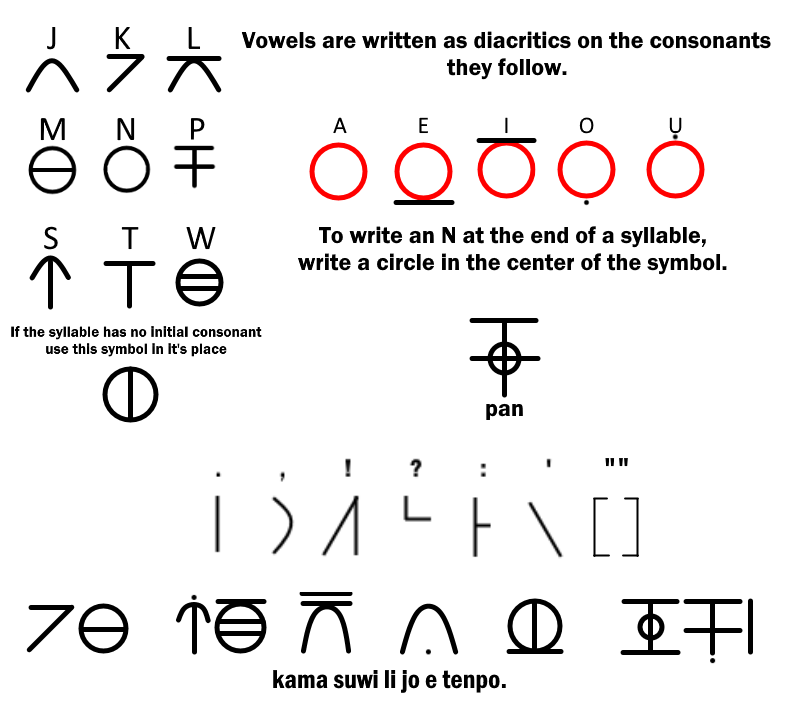
\includegraphics[scale=0.5]{sitelen_pona_pi_jan_Makuwe.png}

%
%%%%%%%%%%%%%%%%%%%%%%%%%%%%%%%%%%%%%%%%%%%%%%%%%%%%%%%%%%%%%%%%%%%%%%%%%%
% eof

%
%%%%%%%%%%%%%%%%%%%%%%%%%%%%%%%%%%%%%%%%%%%%%%%%%%%%%%%%%%%%%%%%%%%%%%%%%%
\bibliography{toki-pona-lessons}
\bibliographystyle{plain}
\printindex
%%%%%%%%%%%%%%%%%%%%%%%%%%%%%%%%%%%%%%%%%%%%%%%%%%%%%%%%%%%%%%%%%%%%%%%%%%
\end{document}
%%%%%%%%%%%%%%%%%%%%%%%%%%%%%%%%%%%%%%%%%%%%%%%%%%%%%%%%%%%%%%%%%%%%%%%%%%
%%%%%%%%%%%%%%%%%%%%%%%%%%%%%%%%%%%%%%%%%%%%%%%%%%%%%%%%%%%%%%%%%%%%%%%%%%
%% eof
